%\documentclass[danish,12pt,a4paper]{report}
\documentclass[danish,12pt,a4paper,twoside, openright]{report}

\usepackage[utf8]{inputenc}					
\usepackage[danish]{babel}	% Dokumentets sprog
\usepackage[T1]{fontenc}		
\usepackage{amsmath,amsthm,amssymb,amsfonts,bm}
\usepackage{ragged2e,anyfontsize}
\usepackage{etex}
\usepackage[titletoc]{appendix}
\usepackage{thmtools}
\usepackage[makeroom]{cancel}
\usepackage{placeins}
\usepackage{multirow}
\usepackage{mathtools}
\usepackage[danish]{varioref}
\usepackage[numbers]{natbib}
\usepackage{dirtytalk}
\usepackage{blindtext}
\RequirePackage{etex}
\usepackage{graphicx}
\usepackage{flafter}
\usepackage{float}
\usepackage{makecell}
\usepackage{lastpage}
\usepackage{fancyhdr}
\usepackage{etoolbox}
\usepackage{mdframed}
\usepackage{multicol}
\usepackage{enumitem}
\usepackage[a4paper]{geometry}
\usepackage{a4wide}
\usepackage{parskip}
\usepackage{booktabs}
\usepackage{rotating}
\usepackage{colortbl}
\usepackage{textcomp}
\usepackage{tabularx}
\usepackage{url}
\usepackage{hyperref}
\usepackage{tasks}
\usepackage{commath}
\usepackage{calc}
\usepackage{indentfirst}
\usepackage[hypcap=false]{caption}
\usepackage[official]{eurosym}
\usepackage{listings}
\renewcommand{\lstlistingname}{Korollar}
\RequirePackage{silence}
\WarningFilter{remreset}{The remreset package}


%matricer 
\usepackage{blkarray}

%Fikser underfull og overfull
\hbadness=10001
\vbadness=10001

%Bibliografi og litteratur
\bibliographystyle{Formalia/vancouver}
\setcitestyle{square}
\usepackage[nottoc,numbib]{tocbibind}

%HERFRA------------
%Symbolregister
\usepackage[intoc, danish]{nomencl}
\makenomenclature
\renewcommand{\nomname}{Symbolregister}
\setlength{\columnsep}{1cm}
\setlength{\nomitemsep}{-1pt}

\makeatletter
\newif\if@nomlist

\newcommand*\nomlist{%
  \@nomlisttrue
  \list{}{%
    \labelwidth\nom@tempdim
    \leftmargin\labelwidth
    \advance\leftmargin\labelsep
    \itemsep\nomitemsep
    \let\makelabel\nomlabel}}

\renewcommand*\thenomenclature{%
  \@ifundefined{chapter}%
    {\section*{\nomname}\if@intoc\addcontentsline{toc}{section}{\nomname}\fi}%
    {\chapter*{\nomname}\if@intoc\addcontentsline{toc}{chapter}{\nomname}\fi}%
  \nompreamble
  \@nomlistfalse
}
\renewcommand\nomgroup[1]{%
  \if@nomlist\endlist\end{multicols}\fi
  \ifx#1A\relax
    \def\nomgroupname{Indledning}%
    \else
    \ifx#1B\relax
    \def\nomgroupname{Sandsynlighed}%
    \else
    \ifx#1C\relax
      \def\nomgroupname{Markov-kæder}%
    \else
    \ifx#1D\relax
      \def\nomgroupname{Beregning af $\bm{e^{tA}}$}%
    \else
    \ifx#1E\relax
      \def\nomgroupname{Stabilitet}%
    \else
    \ifx#1F\relax
      \def\nomgroupname{Problemløsning}% 
      % Her kan man indsætte flere afsnit ved at fortsætte if-else statementet, husk at slutte med \fi for at slutte end-if-else
    \else 
       \def\nomgroupname{Diverse}%
      \fi
      \fi
      \fi
      \fi
    \fi
  \fi
  \begin{multicols}{2}[\raggedcolumns\noindent\large\textbf{\textsf{\nomgroupname}}]
  \nomlist
}
\renewcommand*\nompreamble{}
\renewcommand*\nompostamble{\end{multicols}}
\makeatother
%HERTIL------------------------ danke

%Gør indholdsfortegnelse og bibliografi dansk
\addto\captionsdanish{
	\renewcommand\contentsname{Indholdsfortegnelse}	
	\renewcommand{\bibname}{Bibliografi}
}
%Subsubsections i indholdsfortegnelse (ikke nummereret)


%%%% ORDDELING %%%%
\hyphenation{In-te-res-se e-le-ment}

%Sidehoved
\setlength{\headheight}{15pt}
\pagestyle{fancy}
\fancyhf{}
\renewcommand{\chaptermark}[1]{ \markboth{\thechapter.\ #1}{}}
\fancyheadoffset{0pt}
\lhead{\nouppercase \leftmark}
\rhead{Aalborg Universitet}
\renewcommand{\chaptermark}[1]
        {\markboth{#1}{}}
\renewcommand{\sectionmark}[1]
        {\markright{\thesection\ #1}}
\lfoot[\fancyplain{}{\bfseries\thepage}]
    {\fancyplain{}{}}
\rfoot[\fancyplain{}{}]%
    {\fancyplain{}{\bfseries\thepage}}
\patchcmd{\chapter}{plain}{fancy}{}{}

%Kapiteludseende
\usepackage{xcolor}
\usepackage{titlesec, blindtext, color}
\definecolor{gray75}{gray}{0.75}
\newcommand{\hsp}{\hspace{20pt}}
\titleformat{\chapter}[hang]{\huge\bfseries}{\thechapter\hsp\textcolor{gray75}{|}\hsp}{0pt}{\huge\bfseries}
\titlespacing*{\chapter}{0pt}{5pt}{25pt}

% Define a simple command to use at the start of a table row to make it have a shaded background
\newcommand{\gray}{\rowcolor[gray]{.9}}

\usepackage{textcomp}
\usepackage{url}
\usepackage{hyperref}

%TikZ
\usepackage{tikz}
\usetikzlibrary{automata, positioning}
\usetikzlibrary{matrix}
\usetikzlibrary{decorations.markings}
\usepackage{stackengine}
\usetikzlibrary{arrows, petri, topaths,graphs,graphs.standard,arrows.meta}
\tikzstyle{arrow} = [thick,->,>=stealth]
\usepackage{tkz-berge}
\usepackage[position=top]{subfig}
\usepackage{verbatim}
\usepackage{pgfplots}
\pgfplotsset{compat=1.15}
\tikzset{->-/.style={decoration={
  markings,
  mark=at position #1 with {\arrow{>}}},postaction={decorate}}} % Midtvejspil
\usepackage{pgfplots, pgfplotstable}



%---- pseudocode 
\usepackage{algorithm}
\usepackage[noend]{algpseudocode}

\usepackage{framed}
\definecolor{myGray}{HTML}{F9F9F9}
\renewenvironment{leftbar}[4][\hsize]
{\def\FrameCommand
    {{\color{#2}\vrule width #4pt}
        \hspace{-8pt}
        \fboxsep=\FrameSep\colorbox{#3}}
    \MakeFramed{\hsize#1\advance\hsize-\width\FrameRestore}}
{\endMakeFramed}

\algnewcommand\algorithmicforeach{\textbf{for each}}
\algdef{S}[FOR]{ForEach}[1]{\algorithmicforeach\ #1\ \algorithmicdo}

%Sætninger, definitioner, mm. general stil
\declaretheoremstyle[
    % spaceabove=14pt, 
    % spacebelow=6pt, 
    headfont=\normalfont\bfseries, 
    bodyfont = \normalfont,
    postheadspace=2mm, 
    headpunct={.}]{mystyle}
    
%Sætning    
\declaretheorem[name={Sætning}, style=mystyle,numberwithin=section]{thm}
\newenvironment{thmx}[1]
    {\begin{leftbar}{black}{myGray}{3}\begin{thm}#1}{\end{thm}\end{leftbar}}
%Definition
\declaretheorem[name={Definition}, style=mystyle,sibling=thm]{defni}
\newenvironment{defn}[1]
    {\begin{leftbar}{black}{myGray}{3}\begin{defni}#1}{\end{defni}\end{leftbar}}
%Eksempel
\declaretheorem[name={Eksempel}, style=mystyle,sibling=thm]{exmp}
\newenvironment{eks}[1]
    {\begin{leftbar}{gray}{white}{3}\begin{exmp}#1}{\end{exmp}\end{leftbar}}
%Lemma
\declaretheorem[name={Lemma}, style=mystyle,sibling=thm]{lema}
\newenvironment{lem}[1]
    {\begin{leftbar}{black}{myGray}{3}\begin{lema}#1}{\end{lema}\end{leftbar}}
%Proposition
\declaretheorem[name={Proposition}, style=mystyle,sibling=thm]{prop}
\newenvironment{pro}[1]
    {\begin{leftbar}{black}{myGray}{3}\begin{prop}#1}{\end{prop}\end{leftbar}}
%Korollar
\declaretheorem[name={Korollar}, style=mystyle,sibling=thm]{koro}
\newenvironment{kor}[1]
    {\begin{leftbar}{black}{myGray}{3}\begin{koro}#1}{\end{koro}\end{leftbar}}

%Bevis
\declaretheoremstyle[
    spaceabove=14pt, 
    spacebelow=6pt, 
    headfont=\normalfont\bfseries, 
    bodyfont = \normalfont,
    postheadspace=1mm, 
    qed=$\blacksquare$, 
    headpunct={.}]{bevisstyle}
\declaretheorem[name={Bevis}, style=bevisstyle,numbered=no]{bev}

%Inline graphics
\newlength\myheight
\newlength\mydepth
\settototalheight\myheight{Xygp}
\settodepth\mydepth{Xygp}
\setlength\fboxsep{0pt}
\newcommand*\inlinegraphics[1]{%
  \settototalheight\myheight{Xygp}%
  \settodepth\mydepth{Xygp}%
  \raisebox{-\mydepth}{\includegraphics[height=\myheight]{#1}}}


%Kommandoer, som gør jeres liv nemmere, når I skriver. Pas på med at lave for mange kommandoer selv
%da det kan være træls for jer når I skal indsende MWE (minimal working examples) ind i fx stackexchange
\usepackage{bbm}
\newcommand{\R}{\mathbb{R}}
\newcommand{\1}{\mathbbm{1}}
\newcommand{\Z}{\mathbb{Z}}
\newcommand{\N}{\mathbb{N}}
\newcommand{\C}{\mathbb{C}}
\renewcommand{\d}{\mathrm{d}}
\newcommand{\eps}{\varepsilon}
\newcommand{\e}{\mathrm{e}}
\newcommand{\E}{\mathcal{E}}
\newcommand{\tr}{\mathrm{tr }}
\newcommand{\F}{\mathcal{F}}
\renewcommand{\L}{\mathcal{L}}
\newcommand{\m}{\cdot}

\newcommand{\I}{I} % :))

\def\partautorefname{Del}
\def\chapterautorefname{Kapitel}
\def\sectionautorefname{Afsnit}
\def\subsectionautorefname{Underafsnit}
\def\figureautorefname{Figur}
\def\tableautorefname{Tabel}
\def\algorithmautorefname{Algoritme}
\def\lstinputlistingautorefname{Korollar}
\def\itemautorefname{Sætning}
\def\equationautorefname{Ligning}


\def\env@matrix{\hskip -\arraycolsep
  \let\@ifnextchar\new@ifnextchar
  \array{*\c@MaxMatrixCols c}}
  
\newcolumntype{L}[1]{>{\raggedright\let\newline\\\arraybackslash\hspace{0pt}}m{#1}}
\newcolumntype{C}[1]{>{\centering\let\newline\\\arraybackslash\hspace{0pt}}m{#1}}
\newcolumntype{R}[1]{>{\raggedleft\let\newline\\\arraybackslash\hspace{0pt}}m{#1}}



\newcommand\invisiblesection[1]{%
  \refstepcounter{section}%
  \addcontentsline{toc}{section}{\protect\numberline{\thesection}#1}%
  \sectionmark{#1}}
  
  %---- pseudocode 
 \usepackage{algorithm}
\usepackage[noend]{algpseudocode}
\usepackage{listings}
\usepackage{lineno, blindtext}
\renewcommand{\lstlistingname}{Kildekode}
%\usepackage{algorithm2e}
\renewcommand{\gets}{:=}
%\usepackage{algorithmic}
\usepackage{emptypage}

\raggedbottom

\def\hmath$#1${\texorpdfstring{{\rmfamily\textit{#1}}}{#1}}



\begin{document} 

\hbadness=99999
\vbadness=99999

\newcommand{\clearemptydoublepage}{\newpage{\pagestyle{empty}\cleardoublepage}} 

\pdfbookmark[0]{Front page}{label:frontpage}%
\begin{titlepage}

\thispagestyle{empty}

\newcommand{\HRule}{\rule{\linewidth}{0.5mm}}

\center

\textsc{}\\[2.5cm]
    
\textsc{\textbf{\LARGE Aalborg Universitet}}\\[1.5cm]

\textsc{\textbf{\Large 4. semester}}\\[0.5cm]

\textsc{\textbf{\large Matematik-Økonomi}}\\[0.5cm]

\textsc{\textbf{\large P4-projekt}}\\[0.5cm]

\textsc{\textbf{\large }}\\[0.5cm]

\HRule \\[0.4cm]

{\huge \bfseries Markov Processes and Decision Theory}\\[0.4cm]

\HRule\\[1.5cm]

\textbf{\large 28/05-2021}\\[1cm]

\includegraphics[height=5cm]{Formalia/AAU-logo-stud-DK-RGB.pdf}

\vfill

\end{titlepage}
\pagebreak
\thispagestyle{empty}
\phantom{a}
\clearpage

% Dette er LaTeX-versionen af titelbladet for TNB studenterrapporter
% Filen kræver:
% Universitetets logo:  AAU-logo-stud-UK eller AAU-logo-stud-DK
% Synopsis: En fil ved navn synopsis.tex

% Udarbejdet af: Jesper Nørgaard (jesper@noergaard.eu) 10. april 2012

\phantomsection
\pdfbookmark[0]{Titelblad}{titelblad}
\thispagestyle{empty}

\begin{minipage}[t]{0.48\textwidth}
\vspace*{-25pt}			%\vspace*{-9pt}
\includegraphics[height=4cm]{Formalia/AAU-logo-stud-DK-RGB.pdf}
\end{minipage}
\hfill
\begin{minipage}[t]{0.48\textwidth}
{\small 
\textbf{Institut for Matematiske Fag}\\
Matematik\\
Skjernvej 4A \\
9220 Aalborg Øst \\
\href{http://math.aau.dk}{http://math.aau.dk}}
\end{minipage}

\vspace*{1cm}

\begin{minipage}[t]{0.48\textwidth}
\textbf{Titel:} \\[5pt]\hspace{2ex}
{Markov Processes and Decision Theory}
\bigskip

\textbf{Projekt:} \\[5pt]\hspace{2ex}
P4-projekt
\bigskip

\textbf{Projektperiode:} \\[5pt]\hspace{2ex}
1. februar 2021 - 28 maj 2021
\bigskip

\textbf{Projektgruppe:} \\[5pt]\hspace{2ex}
f21mmf2
\bigskip

\textbf{Deltagere:} \\[5pt]%\hspace*{2ex}
Jonathan Pedersen\\%\hspace*{2ex}
Julie Tømmerby Thomsen\\%\hspace*{2ex}
Mikkel Irgens Prior Nielsen \\%\hspace*{2ex}
Oliver Christensen\\%\hspace*{2ex}
Sandra Helweg Sørensen\\
%Navn6\\%\hspace*{2ex}

\textbf{Vejleder:} \\[5pt]%\hspace*{2ex}
Toke Christian Zinn \\

\textbf{Sidetal: \pageref{LastPage} + forside} \\ 
\textbf{Afsluttet 28/05-2020}

\end{minipage}
\hfill
\begin{minipage}[t]{0.5\textwidth}
\textbf{Synopsis:} \\[5pt]
This paper examines how to determine the optimal consumption and maximal reward for a consumer in a given period. Furthermore, it studies how the probability of unemployment, interest rate and loan affect the optimal consumption and maximal reward. The Consumer Problem is a Markov Decision Process and therefore, the optimal consumption and maximal reward can be determined using backward induction and the Bellman equation. To arrive at this conclusion and to implement the probability of unemployment, it is necessary to introduce basic concepts within probability theory such as conditional probability, expected value and Markov-chains. Moreover, Markov Decision Processes will be examined and implemented within the Consumption Problem using Python.
From this, an inverse relationship between unemployment and total reward has been found, while the reasonable consumer has a positive relationship between consumption and interest rate. Furthermore, the loan restriction and ratio between the lendingrate and depositrate affect the reward and the consumption.




 % Skriv synopsis i dette dokument
\end{minipage}
\hspace*{2ex}

\vfill

{\footnotesize \textit{Rapportens indhold er frit tilgængeligt, men offentliggørelse (med kildeangivelse) må kun ske efter aftale med forfatterne.}}

\pagebreak
\phantom{a}
\thispagestyle{empty}
\clearemptydoublepage

\setcounter{page}{1}
\pagenumbering{roman}
\section*{Forord}
\addcontentsline{toc}{chapter}{\protect\numberline{}Forord}


Projektperioden er forløbet fra 01/02-2021 - 28/05-2021, og er skrevet at matematik-økonomi studerende på Aalborg Universitet. Det antages, at læseren mindst er 4. semesters studerende på en matematisk uddannelse, og kender dermed begreber som konvergens, ligevægt med mere. \\

\large\textbf{Læservejledning} \normalsize \newline
Referencer er skrevet i begyndelsen af hvert afsnit og henviser til litteraturlisten i slutningen af projektet. Henvisninger er skrevet efter Vancouvermetoden, og skrives derfor: [kildenummer, sidetal].     % Vancover-metoden

\bigskip

\textcolor{white}{tekst}

\begin{minipage}[L]{0.45\textwidth}
 \centering
 \rule{\textwidth}{0.5pt}\\
  Jonathan Pedersen\\
 {\footnotesize jlpe19@student.aau.dk}
\end{minipage}
\hfill
\begin{minipage}[H]{0.45\textwidth}
 \centering
 \rule{\textwidth}{0.5pt}\\
  Julie Tømmerby Thomsen\\
 {\footnotesize jtth19@student.aau.dk}
\end{minipage}
\vspace{3\baselineskip}


\begin{minipage}[L]{0.45\textwidth}
 \centering
 \rule{\textwidth}{0.5pt}\\
 Mikkel Irgens Prior Nielsen\\
 {\footnotesize mipn19@student.aau.dk}
\end{minipage}
\hfill
\begin{minipage}[H]{0.45\textwidth}
 \centering
 \rule{\textwidth}{0.5pt}\\
  Oliver Christensen\\\
 {\footnotesize ochri19@student.aau.dk}
\end{minipage}
\vspace{3\baselineskip}


\begin{minipage}[H]{0.45\textwidth}
 \centering
 \rule{\textwidth}{0.5pt}\\
 Sandra Helweg Sørensen\\
 {\footnotesize shsa19@student.aau.dk}
\end{minipage}



\pagebreak
%Symbolregister

% Symbolregisteret kan opdeles som set nedenfor, ved at indsætte \nomenclature[A]{$mit-symbol$}{forklaring} indsættes det under kategori A, kategori kan laves i preamble under symbolregister, hvis ikke et symbol får en kategori gives den "other".

% Eksempel på et symbolregister:

% A = Indledning/Problemanalyse/Problemformulering
\nomenclature[A]{$a$}{Test}

% B = Sandsynlighed
%Mængder
\nomenclature[B,01]{$S$}{Et udfaldsrum}
\nomenclature[B,01]{$s$}{Element af udfaldsrummet}
\nomenclature[B,01]{$A, B$}{Hændelse}
\nomenclature[B,01]{$\Sigma$}{Hændelsesrum}
\nomenclature[B,01]{$\emptyset$}{Den tomme mængde}
\nomenclature[B,01]{$\R$}{De reelle tal}
\nomenclature[B,01]{$P(\cdot)$}{Sandsynlighedsmål}
\nomenclature[B,01]{$A_k, B_k$}{Den $k$'te hændelse}
\nomenclature[B,01]{$P(A | B)$}{Sandsynligheden for $A$ givet $B$}
\nomenclature[B,01]{$k,n,i,j$}{Tællevariabler}
\nomenclature[B,01]{$\E$}{Tilfældigt eksperiment}
\nomenclature[B,01]{$X, Y$}{Diskrete tilfældige variabler}
\nomenclature[B,01]{$Range(\cdot)$}{Billedet af en diskret tilfældig variabel}
\nomenclature[B,01]{$(S,\Sigma, P)$}{Sandsynlighedsrum}
\nomenclature[B,01]{$X^{-1}$}{Urbilledet af $X$}
\nomenclature[B,03]{$p_X(\cdot)$}{Frekvensfunktionen til $X$}
\nomenclature[B,01]{$\mathcal{Y}$}{En mængde}
\nomenclature[B,01]{$F_X(\cdot)$}{Fordelingsfunktion til $X$}
\nomenclature[B,04]{$g(\cdot)$}{Vilkårlig reel funktion funktion}
\nomenclature[B,04]{$E[\cdot]$}{Den forventede værdi}
\nomenclature[B,04]{$Var[\cdot]$}{Varians}
\nomenclature[B,04]{$\sigma$}{Standardafvigelsen}

%Diverse


% C = Differentialligninger
\nomenclature[C,01]{$\frac{d^nx}{dt^n}$}{Leibniz' notation for $n$'te afledte af $x$ med hensyn til $t$}



% \noncleture[BOGSTAV,VÆGT]{symbol}{symbolforklaring}
% Hvor BOGSTAV betegner afsnittet den skal i og VÆGT betegner hvor den skal hen (01 er først og 0n er sidst)

% D = Beregning a e^tA Hej får 9 fejl prøver lige at sætte preamble ind igen
%wut Yessir 












% E = Stabilitet


% F = Problemløsning

% P = Diverse


\printnomenclature[2.5cm]

% Ja præcis den her :))))))))))))

\tableofcontents

\clearpage
\clearemptydoublepage
\setcounter{page}{1}
\pagenumbering{arabic}


%Indsæt her jeres dokumenter. Lav mapper under afsnit, som har jeres kapitelnavne, og indsæt herunder disse mapper jeres .tex dokumenter

\chapter{Indledning} 
    % Input indledningens main-fil her:
    \section{Problemanalyse}

Alle mennesker, som køber og forbruger varer, kan klassificeres som forbrugere. Enhver forbruger har en opsparing og en indkomst, som udgør et muligt forbrug. En forbruger har et basisforbrug, hvilket er det nødvendige forbrug, herunder vand, varme og husleje. Derudover har forbrugere et varierende forbrug, som er den del af forbruget, der bruges på eksempelvis tøj og møbler. Det varierende forbrug afhænger af den marginale forbrugstilbøjelighed, som bestemmer hvor meget af den disponible indkomst, der forbruges. Da basisforbruget er et nødvendigt forbrug, vil den marginale forbrugstilbøjelighed ikke påvirke dette.

Ved at købe varer og ydelser får forbrugeren en tilfredshed, som måles i nytte. Forbrugere er interesseret i at få så meget tilfredshed som muligt. Derfor skal man som forbruger beslutte, hvor meget der skal spares op, og hvor meget der skal forbruges til et givet tidspunkt for at maksimere sin nytte. Disse beslutninger afhænger blandt andet af forbrugerens nuværende økonomi samt forventningerne til den fremtidige økonomi. Forbrugerens økonomi kan blandt andet blive påvirket af arbejdsstatus, løn, pandemier og finanskriser. Disse faktorer påvirker det varierende forbrug, da den disponible indkomst og den marginale forbrugstilbøjelighed ændres. 

Forbrugere er forskellige, hvilket resulterer i, at hver forbruger har deres egen strategi  til at opnå mest mulig nytte. Nogle forbrugere får mere nytte af at forbruge så meget som muligt i nuet og er derfor ligeglade med indlånsrenten. Andre forbrugere er indifferente i forhold til, om der forbruges nu fremfor senere. Denne type forbruger maksimerer sin nytte ved at have et højt samlet forbrug. Ved en positiv indlånsrente vil denne forbruger dermed maksimere sin nytte ved at forbruge alt til sidst. Typisk er forbrugere mere påpasselige med deres forbrug. Forbrugere får derfor ofte mest nytte af at fordele forbruget ud, så der kan forbruges i hver måned. De ovenstående forbrugstilbøjeligheder kaldes henholdsvis utålmodig, tålmodig og fornuftig, og vil uddybes senere i projektet. 

\section{Problemafgrænsing}
Problemet hvor en forbruger skal tage beslutninger over en given tidsperiode for at maksimere sin nytte, kaldes forbrugerproblemet, og kan opstilles som en Markov beslutningsproces.

Denne Markov beslutningsproces er en beslutningsmodel, hvor forbrugeren til hvert beslutningstidspunkt skal vælge, hvor meget der skal forbruges. Beløbet som ikke forbruges spares op og kan dermed forbruges til næste beslutningstidspunkt. Forbrugeren skal til ethvert beslutningstidspunkt vælge det forbrug, som maksimerer nytten over hele tidsperioden. %Dette forbrug kan bestemmes ved at anvende baglæns induktion heriblandt Bellman ligningen. 

I dette projekt vil forbruget ikke blive delt op i basis- og varierende forbrug. Det antages, at forbrugerens løn og forventning til arbejdstatus er fast over tidsperioden. Derfor påvirkes disse faktorer blandt andet ikke af pandemier eller finanskriser. Derudover antages det, at den disponible indkomst er lig lønnen, når forbrugeren er i arbejde og nul i de beslutningstidspunkter, hvor han er arbejdsløs. Den disponible indkomst påvirkes dermed ikke af skatteændringer. Sandsynligheden for at være i arbejde vil blive beskrevet ved en Markov-kæde, hvor forbrugerens arbejdsstatus i næste tidsskridt kun afhænger af hans arbejdsstatus i nuværende tidsskridt.

Dette projekt tager udgangspunkt i den fornuftige forbruger, der opnår størst mulig nytte ved at fordele sit forbrug ligeligt mellem beslutningstidspunkterne. Det antages, at det optimale forbrug til hvert beslutningstidspunkt udelukkende afhænger af sandsynligheden for at blive arbejdsløs, forblive arbejdsløs, opsparing og indlånsrente. Når muligheden for at låne penge tilføjes, afhænger forbruget til hvert beslutningstidspunkt også af dette, samt udlånsrenten.

Det er derfor interessant at undersøge, hvordan forbrugerens nytte og forbrug til hvert beslutningstidspunkt påvirkes, hvis sandsynligheden for at blive arbejdsløs, indlånsrenten og muligheden for at låne varierer. 


%For at kunne beskrive Markov-kæderne for forbrugerens %arbejdsstatus og Markov beslutningsprocessen vil der %introduceres begrebet forventet værdi. Derudover %præsenteres begreber som tilfældige variabler og %sandsynlighedsrum.

%for at kunne beskrive forventet værdi, Markov kæder og %Markovbeslutningsprocesser. 

Ud fra ovenstående problemafgrænsning opstilles følgende problemformulering.





 





\section{Problemafgrænsning}
Hvad vælger vi at begrænse os til? Tekst her Tekst her Tekst her Tekst her Tekst her Tekst her Tekst her Tekst her Tekst her Tekst her 

\section{Problemformulering}

En super god problemformulering - Tekst her Tekst her Tekst her 






\chapter{Sandsynlighed}\label{kapitel:sandsynlighed}
I dette kapitel anvendes \cite[s. 1-111]{olofsson2005probability} og \cite[s. 6-32]{oxford}. 

Sandsynlighedsteori kan anvendes inden for blandt andet matematik og økonomi til at beregne sandsynligheden for forskellige udfald. I dette projekt tages der udgangspunkt i en forbruger, hvis arbejdsstatus er beskrevet ved en Markov-kæde. 
For at kunne definere og analysere Markov-kæder introduceres nogle grundlæggende begreber inden for sandsynlighedsteori. Disse begreber defineres i dette kapitel. 

\section{Introduktion}
%To primære fortolkninger af sandsynlighed er, at en sandsynlighed er grænsen for den relative frekvens eller en vis grad af tro. Ud over disse to fortolkninger er det muligt at formulere en matematisk definition af, hvad sandsynlighed er.


%

%Hvis man kaster en mønt vil de fleste mene at der er $50\%$ chance for at den lander på krone. Derudover kan man kaste mønten mange gange og se at ca halvdelen af gangene man kaster mønten rammer den krone. I dette afsnit vil en matematiske definition på sandsynlighed præsenteres, og det vil være denne definition som fremadrettet vil blive anvendt.

%I dette projekt defineres sandsynlighed aksiomatisk
%Endeligt, er det muligt at formulere en matematisk definition af, hvad sandsynlighed er.


%Derudover bliver ordet sandsynlighed brugt om hvad en person tror vil være 



%For at kunne beskrive en sandsynlighed matematisk skal begreber som \textit{tilfældighed}, \textit{udfaldsrum}, \textit{hændelser} og \textit{hændelsesrum} først beskrives.

Noget kaldes \textit{tilfældigt}, hvis det ikke er muligt at forudse udfaldet. Hvis der udføres et eksperiment, hvor udfaldet er tilfældigt, kaldes det et \textit{tilfældigt eksperiment}, $\E$. Et eksempel på et tilfældigt eksperiment er et terningkast, hvor det ikke er sikkert, hvorvidt udfaldet er $1, 2, \dots$ eller $6$. %%For et tilfældigt eksperiment defineres begreberne, \textit{udfaldsrum}, \textit{hændelser} og \textit{hændelsesrum} som følgende

Mængden af mulige udfald i et tilfældigt eksperiment, $\E$, kaldes et \textit{udfaldsrum} og noteres $\Omega$. Et udfaldsrum kan bestå af en \textit{endelig}, \textit{tællelig uendelig} eller en \textit{ikke-tællelig uendelig} mængde af udfald. Hvis udfaldene er adskilt i punkter, eksempelvis $\{1,2,3, \dots\}$, er det et tælleligt udfaldsrum, og hvis det derimod er et kontinuum af punkter, er det ikke-tælleligt. Eksempelvis er udfaldsrummet $[0, 10]$ ikke-tælleligt.

Ud fra udfaldsrummet defineres begrebet \textit{hændelsesrum} og \textit{hændelse} som følgende.

\begin{defn}\textbf{Hændelsesrum}
\newline
    Mængden af delmængder af udfaldsrummet, $\Omega$, kaldes et hændelsesrum og noteres $\mathcal{F}$, hvis
    \begin{enumerate}
        \item $\F$ er ikke-tom,
        \item $A\in\F$, så er $A^c=\Omega\backslash A \in \mathcal{F}$,
        \item $A_1, A_2,\dots\in \F$, så er $\displaystyle \bigcup_{k=1}^\infty A_k\in\F$.
    \end{enumerate}
Elementerne, $A\in \F$, kaldes for hændelser.
\end{defn}

Hvis der for to hændelser $A$ og $B$ gælder, at $A \cap B = \varnothing$, kaldes hændelserne for \textit{disjunkte}.

Det er ud fra ovenstående muligt at definere et \textit{sandsynlighedsmål}.

\begin{defn}\textbf{Sandsynlighedsregningens aksiomer} \label{def:sandsynlighedsregningens_grundsætninger}%Ny definition
\newline
Lad $\Omega$ være et udfaldsrum, $\F$ et hændelsesrum og $A$ en hændelse. En funktion,\\ $P: \F \to [0,1]$, kaldes et sandsynlighedsmål på $(\Omega, \F)$, hvis
\begin{enumerate}
    \item $0 \leq P(A) \leq 1$,
    \item $P(\Omega) = 1$ og $P(\emptyset)=0$,
    \item $(A_1, A_2, \ldots) $ er en sekvens af parvise disjunkte hændelser, altså $A_i \cap A_j = \emptyset$ for $i \neq j$, så er
    \begin{align*}
        P\left(\bigcup_{k=1}^\infty A_k \right) = \sum_{k=1}^\infty P(A_k).
    \end{align*}
\end{enumerate}
\end{defn}

Jævnfør punkt 3 i \autoref{def:sandsynlighedsregningens_grundsætninger} følger det, at
\begin{align*}
    P\left(\bigcup_{k=1}^n A_k \right) = \sum_{k=1}^n P(A_k),
\end{align*}
ved at lade $A_k = \emptyset$ for $k > n$.

Ud fra udfaldsrum, hændelsesrum og sandsynlighedsmål defineres \textit{sandsynlighedsrum} som følgende

\begin{minipage}\textwidth
\begin{defn}\textbf{Sandsynlighedsrum} \label{def:sandsynlighedsrum}\\
    Lad $\Omega$ være et udfaldsrum, $\mathcal{F}$ et hændelsesrum og $P$ et sandsynlighedsmål på $(\Omega, \F)$. Så er sandsynlighedsrummet givet ved triplen, $(\Omega, \F, P)$. 
\end{defn}
\end{minipage}







\section{Betinget sandsynlighed}
Hvis man har ekstra information om en given hændelse, så vil udfaldsrummet indskrænkes - mere formelt:\\
\begin{minipage}\textwidth
\begin{defn}\textbf{Betinget sandsynlighed} %Ny definition
\newline
Lad $B$ være en hændelse sådan at $P(B)>0$. Den \textit{betingede sandsynlighed} af $A$ givet $B$ er defineret som
\begin{align*}
      \displaystyle P(A|B)=\frac{P(A\cap B)}{P(B)}
\end{align*}
\end{defn}
\end{minipage}

\subsection{Uafhængige hændelser}
Hvis to hændelser, $A$ og $B$, er \textit{uafhængige}, vil en betingelse $B$ ikke påvirke sandsynligheden for $A$. Med andre ord, så er den betingede og ubetingede sandsynlighed den samme. Dette har konsekvensen, at $P(A)=P(A|B)\Leftrightarrow P(A\cap B)=P(A)P(B)$. Faktisk kan dette generaliseres til følgende definition:\\
\begin{minipage}\textwidth
\begin{defn}\textbf{Uafhængighed} %Ny definition
\newline
Hændelserne, $A_1,A_2,\dots$ siges at være uafhængige hvis
\begin{align*}
    P(A_{i_1}\cap A_{i_2}\cap\cdots\cap A_{i_k})=P(A_{i_1})P(A_{i_2})\cdots P(A_{i_k})
\end{align*}
for alle følger af heltal, $i_1<i_2<\cdots<i_k, k=2,3,\dots$.
Hvis de ikke er uafhængige er \textit{afhængige}.
\end{defn}
\end{minipage}
\subsection{Total sandsynlighed}
I tilfælde af, at sandsynligheden for en given hændelse er svær at bestemme direkte kan det i nogle tilfælde være hensigtsmæssigt at opdele problemet i termer af betinget sandsynlighed.



\begin{minipage}\textwidth
\begin{thmx} \textbf{Loven om Total Sandsynlighed} \label{sæt:loven_om_total_sandsynlighed} %Ny sætning
\newline
Lad $B_1,B_2,\dots$ være en følge af hændelser, sådan at
\begin{enumerate}[label=(\textbf{\alph*})]
\item $P(B_k)>0$ for $k=1,2,\dots$
\item $B_i$ og $B_j$ er disjunkte når $i\neq j$
\item $S=\bigcup_{k=1}^\infty B_k$
\end{enumerate}
Så for enhver hændelse, $A$ gælder der, at
\begin{align*}
    P(A)=\sum_{k=1}^\infty P(A|B_k)P(B_k)
\end{align*}
\end{thmx}
\end{minipage}
\begin{bev} \textbf{} %Nyt bevis
\newline
Bemærk, at
\begin{align*}
    A=A\cap S=\bigcup_{k=1}^\infty(A\cap B_k)
\end{align*}
i henhold til den distributive lov for uendelige foreningsmængder (se Bilag \ref{Distributive love}). 
Eftersom $A\cap B_1,A\cap B_2,\dots$ er parvis disjunkte fås
\begin{align*}
    P(A)=\sum_{k=1}^\infty P(A\cap B_k)=\sum_{k=1}^\infty P(A|B_k)P(B_k)
\end{align*}
\end{bev}
%By virtue of Proposition 1.2, we realize that the law of total probability is also true for a finite union of events
%Hvis mængden af hændelser er endelig og givet ved $n$, kan man konstruere en uendelig følge af hændelser, sådan at P(\bigcup_{k=n}^\infty B_k)=0.
For $n=2$ gælder der, at hvis $B_1=B$, så følger det at $B_2=B^c$ og følgende korollar fås.
\begin{minipage}\textwidth
\begin{kor} \textbf{} %Nyt korollar
\newline
Hvis $0<P(B)<1$, så er
\begin{align*}
    P(A)=P(A|B)P(B)+P(A|B^c)P(B^c)
\end{align*}
\end{kor}
\end{minipage}
\iffalse
Idét foreningsmængder er kommutative, gælder der, at
$$P(B_j|A)P(A)=P(A|B_j)P(B_j)$$
som må betyde, at
$$P(B_j|A)=\frac{P(A|B_j)P(B_j)}{P(A)}$$

Dette leder op til følgende proposition:\\
\begin{minipage}\textwidth
\begin{pro} \textbf{(Bayes' Formel).} %Ny proposition
\newline
Med samme antagelser som i Loven om Total Sandsynlighed og hvis $P(A)>0$, så gælder der for enhver hændelse, $B_j$, at
\begin{align*}
    P(B_j|A)=\frac{P(A|B_j)P(B_j)}{\sum_{k=1}^\infty P(A|B_k)P(B_k)}
\end{align*}
\end{pro}
\end{minipage}
\begin{bev}
Beviset følger af foregående udregninger.
\end{bev}

Analogt, følger denne korrollar:\\
\begin{minipage}\textwidth
\begin{kor} \textbf{} %Nyt korollar
\newline
Hvis $0<P(B)<1$ og $P(A)>0$, så er
\begin{align*}
    P(B|A)=\frac{P(A|B)P(B)}{P(A|B)P(B)+P(A|B^c)P(B^c)}
\end{align*}
\end{kor}
\end{minipage}
\fi

\section{Tilfældige variabler}

$S = \{1,2,3\}$
$\Sigma = \{\emptyset, \{ 1\}, \{ 2\}, \{ 3\},  \{ 1, 2\}, \{ 2,3 \}, \{ 1,3\}, S\}$
\pagebreak
Tilfældig variabel:\\
En tilfældig variabel på $(S,\Sigma, P)$ er en funktion $X:S\to \R$ således at:\\
$\forall x\in \R : \{s \in S: X(s)\leq x\} \in \Sigma$

Tilfældig diskret variabel:\\
Billedet er en tællelig delmængde af $\R$\\
$\forall x\in \R : \{s \in S: X(s) = x\} \in \Sigma$


\begin{minipage}\textwidth
\begin{defn}\textbf{Hændelsesrum}\\
    Lad $S$ være et udfaldsrum for et eksperiment $\E$.
    
    Hændelsesrummet er givet ved potensmængden
    $\Sigma = \{A:A\subseteq S\}$.
\end{defn}
\end{minipage}
derved er hændelsesmængden givet ud fra alle mulige hændelser

\begin{minipage}\textwidth
\begin{defn}\textbf{Sandsynlighedsrum}\\
    Lad $S$ være et udfaldsrum, $A$ et hændelsesrum til $S$ og $P$ et sandsynlighedsmål over hændelsesrummet. 
    
    Så er sandsynlighedsrummet givet ved tretupelen $(S, \Sigma, P)$ for et eksperiment, $\E$.
\end{defn}
\end{minipage}


% \begin{minipage}\textwidth
% \begin{defn}\textbf{Tilfældig variabel} %Ny definition
% \newline
% En tilfældig variabel er en variabel, $x\in \R$, der får sin værdi fra et tilfældigt eksperiment.
% \end{defn}
% \end{minipage}

% \begin{minipage}\textwidth
% \begin{defn}\textbf{Tilfældig variabel} %Ny definition
% \newline
% Lad $\E$ være et eksperiment med sandsynlighedsrummet $(S, \Sigma, P)$.

% Så er en tilfældig variabel en funktion på sandsynlighedsrummet $X:S\to \R$.


% \end{defn}
% \end{minipage}


En tilfældig variabel, $X$, er en reel variabel som får sin værdi fra et eksperiment. 
Tilfældige variabler kan udtrykkes som reelle funktioner, der tildeler reelle værdier til de mulige udfald af eksperimentet.

%En tilfældig variabel er en variabel, $X$, der først tildeles en værdi efter eksperimentet er udført. 
Da $X$ først antager en værdi efter eksperimentet, er det kun muligt at beskrive billedet af $X$, som er mængden af mulige værdier $X$ kan antage, samt de  tilhørende sandsynligheder. Billedet af $X$ betegnes $range(X)$ og de tilhørende sandsynligheder kaldes for \textit{fordelingen} af $X$.

% Før eksperimentet er det muligt at beskrive mængden af mulige værdier, $range(X)$, og de tilhørende sandsynligheder, \textit{fordelingen} af $X$.
% Det betyder, at det er muligt at beskrive billedet af $X$, men ikke hvilken værdi $X$ antager.

\begin{minipage}\textwidth
\begin{defn}\label{def:Diskret_tilfældig_variabel}\textbf{Diskret tilfældig variabel} %Ny definition
\newline
Lad $(S, \Sigma, P)$ være et sandsynlighedsrum. En diskret tilfældig variabel $X$ er en reel funktion på sandsynlighedsrummet $X:S\to \R$ således, at
%
\begin{align}
    &\text{$Range(X)$ er en tællelig delmængde af $\R$ } \quad \text{og}\label{eq:def_diskretitet_betingelsen}\\
    &\forall x\in \R: \{s\in S: X(s)=x\}\in % S\cup \{\emptyset\} \subseteq 
    \Sigma\label{eq:def_tilfældig_variabel}
\end{align}

\end{defn}
\end{minipage}


At en funktion er diskret betyder, at dens billede er tællelig. 
I \autoref{def:Diskret_tilfældig_variabel} er
\eqref{eq:def_diskretitet_betingelsen} betingelsen, der sikrer, at $X$ er en diskret funktion.

%Dette betyder, at \eqref{eq:def_diskretitet_betingelsen} er betingelsen, der sikrer, at $X$ er diskret.  


% Betingelse (2,2):\\ 
% Da den værdi en diskret variabel $X$ antager, ikke kan forudsiges, 



% En diskret variabel $X$ antager værdier fra $\R$, men man kan ikke forudsige værdien af $X$ før eksperimentet er udført.

% Af denne grund, vil vi finde sandsynligheden for at $X$ er en given værdi $x$. 

%Det bemærkes, at $X$ antager værdien $x$ hvis og kun hvis resultatet af eksperimentet ligger i delmængden som afbilledes over i $x$ - altså delmængden $X^{-1}(x) = \{s\in S: X(s)=x\}$. Betingelse (2,2) postulerer at alle sådanne delmængder er hændelser, og da alle kombinationer af hændelser er i $\Sigma$, kan en tilsvarende sandsynlighed findes.

Det bemærkes, at $X$ antager værdien $x$ hvis og kun hvis resultatet af eksperimentet, $\E$, ligger i en delmængde af $S$ som afbilledes over i $x$. Derved ligger resultatet af $\E$ i delmængden $X^{-1}(x) = \{s\in S: X(s)=x\} \subseteq S\cup \{\emptyset\}$, hvor det bemærkes, at  $X^{-1}(x)\subseteq S\cup \{\emptyset\} \subseteq \Sigma$.
Betingelse \eqref{eq:def_tilfældig_variabel} gør derfor, at alle sådanne delmængder er elementer af hændelsesrummet, $\Sigma$, og derfor har en tilsvarende sandsynlighed, $P$.

Da den diskret tilfældige variabel kan antage flere værdier, defineres en funktion, der bestemmer sandsynligheden for hvert udfald af den diskret tilfældige variabel.

Fremadrettet vil $\{s\in S: X(s)=x\}$ blive betegnet $\{X=x\}$.

\begin{minipage}\textwidth
\begin{defn}\label{def:Frekvensfunktionen}\textbf{Frekvensfunktionen} %Ny definition
\newline
    Lad $X$ være en diskret tilfældig variabel. % med range $\{x_k| k\in N \subseteq \N\}$. 
    Funktionen $p_X:\R\to [0,1]$ defineret ved
%    
    $$ p_X(x) = P(X = x)$$
%    
    kaldes for \textit{frekvensfunktionen} eller \textit{pmf} til $X$.
\end{defn}
\end{minipage}

Frekvensfunktionen er derved sandsynligheden for at afbildingen $X$ antager værdien $x$.
Hvis en hændelse ikke er element af $range(X)$ vil frekvensfunktionen give $0$. 
%$p_X(x)=0$ for $x\notin range(X)$.

\begin{minipage}\textwidth
\begin{pro}\label{prop:frekvensfunktion}\textbf{}\\
    Lad $X$ være en diskret tilfældig variabel og lad $p_X$ være den tilhørende frekvensfunktion. Så gælder det, at
    %
   % En funktion $p_X$ er en frekvensfunktion for en diskret tilfældig variable $X$, %  med $range(X)=\{x_k | k\in N \subseteq \N\}$
    %hvor det gælder, at
    \begin{enumerate}
        \item[(a)] $\displaystyle p_X(x)\geq 0$
        %\item[(b)] $\displaystyle \sum_{k=1}^\infty p(x_k)=1$
        \item[(b)] $\displaystyle \sum_{x\in \R} p_X(x)=1$
    \end{enumerate}
    %hvor summen er endelig, hvis $range(X)$ er endelig.
    for alle $x\in \R$.
\end{pro}
\end{minipage}

\begin{bev} \textbf{} %Nyt bevis
\newline
Lad $X$ være en diskret tilfældig variabel der kan antage værdier $x\in\R$ og lad $p_X(x)$ være en frekvensfunktion til $X$.
\begin{itemize}
    \item []\textbf{Bevis for punkt (a)}\\
    % Antag først at, $x\in Range(X)$, så vil frekvensfunktionen være sandsynligheden for at $X$ giver hændelsen $x$. Fra \autoref{def:sandsynlighedsregningens_grundsætninger} punkt (a) fås, at enhver hændelse har en ikke-negative sandsynlighed, og derfor må $p_X(x) = P(X=x) \geq 0$. \\
    % Antag omvendt, at $x\notin Range(X)$, så vil det være en umulig hændelse, at $X$ giver hændelsen $x$. Da sandsynligheden af en umulig hændelse altid er 0, fås $p_X(x)=P(\emptyset) = 0$.\\
    % Derved er det bevist, at $p_X(x) \geq 0$
    % 
    Da $x\in \R$, er frekvensfunktionen defineret over alle $x$ og angiver sandsynligheden for, at $X$ giver hændelsen $x$. Fra \autoref{def:sandsynlighedsregningens_grundsætninger} punkt (a) fås, at enhver hændelse har en ikke-negative sandsynlighed, og derfor må $p_X(x) = P(X=x) \geq 0$.
    Derved er det bevist, at $p_X(x) \geq 0$
    
    \item[]\textbf{Bevis for punkt (b)}\\
    Lad $ \sum_{x\in \R} p_X(x)$ være givet.
    Summen omskrives ved brug af \autoref{def:Frekvensfunktionen}.
    \begin{align*}
    \sum_{x\in \R} p_X(x) &=  \sum_{x\in \R} P(X=x)
    \intertext{Dette omskrives ved brug af  \autoref{def:sandsynlighedsregningens_grundsætninger} punkt (c)}
     \sum_{x\in \R} P(X=x)  &= P\left( \bigcup_{x\in \R} \{X=x\}\right)\\
    &= P\left( \bigcup_{x\in \R} \{s\in S: X(s)=x\}\right) \\
    &= P\left( \bigcup_{x\in Range(X)} \{s\in S: X(s)=x\}\right) + P\left( \bigcup_{x\notin Range(X)} \{s\in S: X(s)=x\}\right)\\
     %P\left( S\cup \emptyset \right) = P(S) + P(\emptyset) 
    &= P(S) + P(\emptyset)
\end{align*} 
    Fra \autoref{def:sandsynlighedsregningens_grundsætninger} punkt (b) gælder det, at $P(S)=1$ og $P(\emptyset)=0$. Det er dermed bevist, at $\displaystyle \sum_{x\in \R} p_X(x)=1$.
\end{itemize}
\end{bev}

Hvis frekvensfunktionen har den samme værdi for alle de mulige udfald er det en uniform fordeling. \\
Frekvensfunktionen kan illustreres i et pindediagram, hvor søjlerne er de forskellige udfald, og højden af en given søjle repræsenterer sandsynligheden for udfaldet.
\textbf{overvej eksempel der viser pindediagram/sim}

\begin{eks} \textbf{} %Nyt eksempel
\newline
I et eksperiment $\E$ kastes to fair terninger. \\ $S=\left\{\{1,1\},\{1,2\},\cdots,\{6,6\}\right\}$ hvor $|S|=6^2 = 36$
%$S = \{2, 3, 4, 5, 6, 7, 8, 9, 10, 11, 12\},$
Lad $X$ være summen af de to terningkast og lad $X$ være givet således, at $Range(X)=\{2, 3, 4, 5, 6, 7, 8, 9, 10, 11, 12\}$.
Sandsynlighederne for at ${X=x}$ kan findes med frekvensfunktionen, hvor  $p_X(2)=\frac{1}{36}, p_X(3)=\frac{2}{36}, \cdots, p_X(12)=\frac{1}{36}$ 


    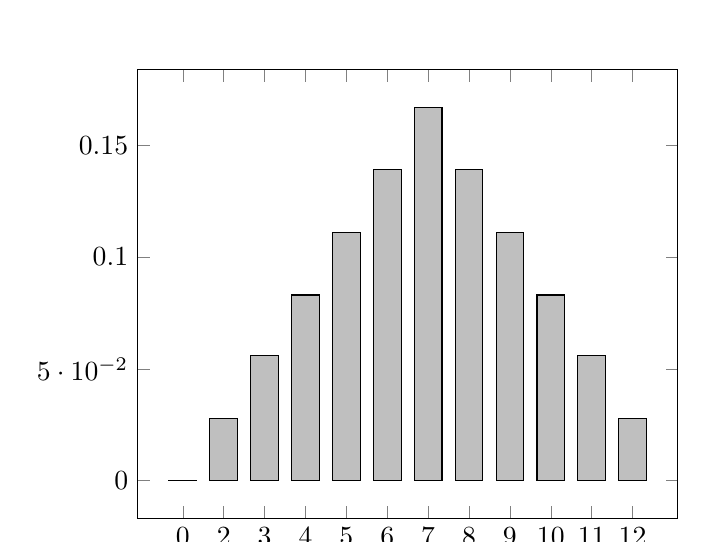
\begin{tikzpicture}
        \begin{axis}[
            symbolic x coords={0, 2, 3, 4, 5, 6, 7, 8, 9, 10, 11, 12},
            xtick=data
          ]
            \addplot[ybar,fill=lightgray] coordinates {
                (0, 0.0000001)
                (2, 0.028)
                (3,  0.056)
                (4,   0.083)
                (5,   0.111)
                (6,  0.139)
                (7,   0.167)
                (8,   0.139)
                (9,  0.111)
                (10,   0.083)
                (11,   0.056)
                (12,  0.028)
            };
        \end{axis}
    \end{tikzpicture}
    

\begin{tikzpicture}
\begin{axis}
\addplot+[ycomb, color=black] plot coordinates
	{(0,3) (1,2) (2,4) (3,1) (4,2)};
\end{axis}
\end{tikzpicture}

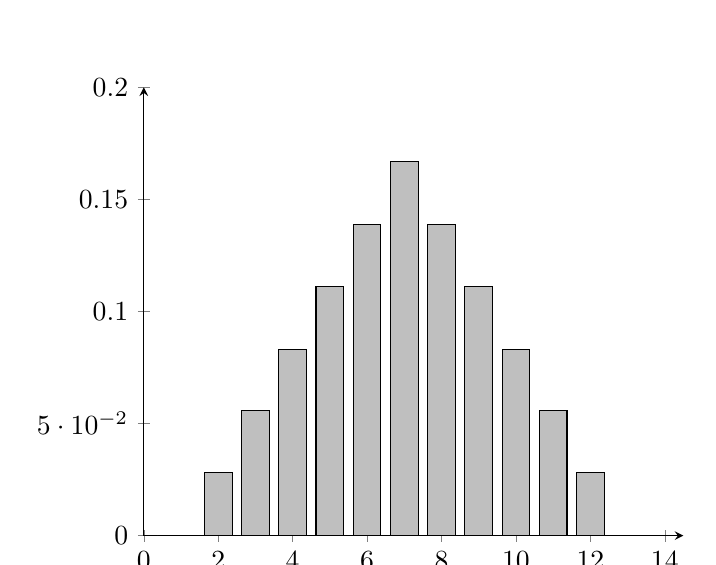
\begin{tikzpicture}
\begin{axis}[axis x line=bottom,
	axis y line=left, ymax=0.2, ymin=0, xmax=14.5, xmin=0]
\addplot [ybar, color=black, fill=lightgray] coordinates
	{           (0, 0)
	            (1, 0)
                (2, 0.028)
                (3,  0.056)
                (4,   0.083)
                (5,   0.111)
                (6,  0.139)
                (7,   0.167)
                (8,   0.139)
                (9,  0.111)
                (10,   0.083)
                (11,   0.056)
                (12,  0.028)}
                (13, 0)
                (14, 0);
\end{axis}
\end{tikzpicture}

% \begin{align*}
%     % p_X(2)=\frac{1}{36}; \quad  p_X(3)=\frac{2}{36}; \quad p_X(4)=\frac{3}{36}; \quad  p_X(5)=\frac{4}{36}; \quad
%     % p_X(6)=\frac{5}{36}\\
%     % p_X(7)=\frac{6}{36}\\
%     % p_X(8)=\frac{5}{36}\\
%     % p_X(9)=\frac{4}{36}\\
%     % p_X(10)=\frac{3}{36}\\
%     % p_X(11)=\frac{2}{36}\\
%     % p_X(12)=\frac{1}{36}\\
% \end{align*}

\end{eks}

%$\Sigma = {{}, {1}, {2}, {3}, {4}, {5}, {6}, {1, 2}, {1, 3}, {1, 4}, {1, 5}, {1, 6}, {2, 3}, {2, 4}, {2, 5}, {2, 6}, {3, 4}, {3, 5}, {3, 6}, {4, 5}, {4, 6}, {5, 6}, {1, 2, 3}, {1, 2, 4}, {1, 2, 5}, {1, 2, 6}, {1, 3, 4}, {1, 3, 5}, {1, 3, 6}, {1, 4, 5}, {1, 4, 6}, {1, 5, 6}, {2, 3, 4}, {2, 3, 5}, {2, 3, 6}, {2, 4, 5}, {2, 4, 6}, {2, 5, 6}, {3, 4, 5}, {3, 4, 6}, {3, 5, 6}, {4, 5, 6}, {1, 2, 3, 4}, {1, 2, 3, 5}, {1, 2, 3, 6}, {1, 2, 4, 5}, {1, 2, 4, 6}, {1, 2, 5, 6}, {1, 3, 4, 5}, {1, 3, 4, 6}, {1, 3, 5, 6}, {1, 4, 5, 6}, {2, 3, 4, 5}, {2, 3, 4, 6}, {2, 3, 5, 6}, {2, 4, 5, 6}, {3, 4, 5, 6}, {1, 2, 3, 4, 5}, {1, 2, 3, 4, 6}, {1, 2, 3, 5, 6}, {1, 2, 4, 5, 6}, {1, 3, 4, 5, 6}, {2, 3, 4, 5, 6}, {1, 2, 3, 4, 5, 6}}$

\textit{Indtil videre} har hændelsen været på formen $\{X=k\}$, hvor $X$ har antaget én bestemt værdi, $k$. Dette kan udvides til hændelser på formen $\{X\leq k\}$, hvor $X$ antager værdier mindre eller lig $k$. Dette kan defineres som følgende funktion

\begin{minipage}\textwidth
\begin{defn}\textbf{Kumulative fordelingsfunktion} %Ny definition
\newline
Lad $X$ være en tilfældig variabel. Funktionen 
$$F(x)=P(X\leq x), \quad x\in\R$$
kaldes for den kumulative fordelingsfunktion (cdf) af $X$
\end{defn}
\end{minipage}

%A real random variable is a real valued function from the possible outcome of a random experiment.

\begin{minipage}\textwidth
\begin{pro} \textbf{} %Ny proposition
\newline
Lad $X$ være en diskret tilfældig variabel med $range(X)=\{x_k | k\in N \subseteq \N\}$, frekvensfunktion, $p$, og kumulative fordelingsfunktion, $F$. Så gælder det, at
\begin{enumerate}
    \item $\displaystyle F(x)=\displaystyle\sum_{k:x_k\leq x}p(x_k), \quad x\in\R$
    \item $\displaystyle p(x_k)=F(x_k)-\lim_{y\uparrow x_k} F(y), \quad k=1, 2,\cdots$
    \item For $B\subseteq \R$, $\displaystyle P(X\in B)=\displaystyle\sum_{k:x_k\in B}p(x_k)$
\end{enumerate}
\end{pro}
\end{minipage}

%\section{Fordelinger - Mikkel}
%\input{Afsnit/Sandsynlighed/Fordelinger}

\section{Forventet værdi og varians}



%\textit{Den forventede værdi} afhænger af de gennemsnitlige værdier af et eksperiment. 
Ud fra frekvensfunktionen, er det muligt at bestemme den \textit{forventede værdi} for en diskret tilfældig variabel. Den forventede værdi afhænger af de gennemsnitlige værdier for de diskrete tilfældige variabler i et tilfældigt eksperiment, $\E$. Den forventede værdi defineres som følgende.

\begin{minipage}\textwidth
\begin{defn}\textbf{Forventet værdi} \label{def:Forventetværdi} %Ny definition 
\newline
Lad $X$ være en diskret tilfældig variabel med den tilhørende frekvensfunktion $p_X$. Den forventede værdi af $X$ er defineret ved
\begin{align}
E[X]=\sum_{x\in \text{Range}(X)} x p_X(x),
\end{align}
hvis summen er absolut konvergent.
\end{defn}
\end{minipage}

Den forventede værdi er et vægtet gennemsnit af de mulige værdier af $X$ med tilsvarende sandsynligheder som vægte. 

Den forventede værdi af en funktion, som afhænger af $X$, kan opstilles som følgende

\begin{minipage}\textwidth
\begin{pro} \textbf{} \label{prop:forventet_værdi_af_funktion} %Ny proposition
\newline
Lad $X$ være en diskret tilfældig variabel med den tilhørende frekvensfunktion $p_X$. Lad $g: \R \to \R$ være en reel funktion. Så gælder det, at
\begin{align}           
    E\left[g(X)\right]=\sum_{x \in \text{Range}(X)} g(x)p_X(x),
\end{align}
hvis summen er absolut konvergent.
\end{pro}
\end{minipage}

\begin{bev}\textbf{} %Nyt bevis
\newline
Lad $(\Omega, \F, P)$ være et sandsynlighedsrum og $X: \Omega \to \R$ være en diskret tilfældig variabel med frekvensfunktion, $p_X$. Lad $I= \text{Range}(X)$ og $Y=g(X)$, så er $Y$ en diskret tilfældig variabel med billede $\text{Range}\hspace{-2pt}\left(g(I)\right)$ og den tilhørende frekvensfunktion $p_Y$. Fra \autoref{def:Frekvensfunktionen} og \autoref{def:Diskret_tilfældig_variabel} gælder det, at
%
\begin{align*}
    p_Y(y) = P(Y = y) = P\left(\{\omega \in \Omega: Y(\omega) = y\}\right).
\end{align*}
%
Af \autoref{def:Forventetværdi} følger det, at
%
\begin{align}\label{eq:E[Y]}
    E[Y] = \sum_{y \in \text{Range}\left(g(I)\right)} yp_Y(y).
\end{align}
%
For ethvert $y\in \text{Range}\hspace{-2pt}\left(g(I)\right)$ eksisterer der mindst et $x\in I$ således, at $g(x)=y$. Dette medfører, at
% 
\begin{align*}
    P\left(\{\omega \in \Omega: Y(\omega) = y\}\right) = P\left(\left\{\omega \in \Omega: X(\omega) \in \{x\in I| g(x)=y\}\right\}\right).
\end{align*}
Derudover gælder det, at
\begin{align*}
    \left\{\omega \in \Omega: X(\omega) \in \{x\in I| g(x)=y\}\right\} = \bigcup_{\substack{x \in I:\\ g(x) =y}} \{\omega \in \Omega |X(\omega) = x\}.
\end{align*}
Hvorom det gælder, at
\begin{align*}
    \{\omega \in \Omega | X(\omega)=x_j\} \cap \{\omega \in \Omega | X(\omega)=x_i\} = \emptyset \text{ for alle } i,j=1,2, \ldots \Rightarrow x_j\neq x_i.
\end{align*}
Det følger da af \autoref{def:ovegangsmatrice} punkt 3 og \autoref{def:Frekvensfunktionen}, at
\begin{align}
    P\left(\left\{\omega \in \Omega: X(\omega) \in \{x\in I| g(x)=y\}\right\}\right)&=\sum_{\substack{x \in I:\\ g(x) =y}} P\left(\{\omega \in \Omega |X(\omega) = x\}\right)\nonumber\\
    &=\sum_{\substack{x \in I:\\ g(x) =y}}p_X(x).\label{eq:bevis_for_forventet_værdi_som_funktion_2}
\intertext{Ved at indsætte \eqref{eq:bevis_for_forventet_værdi_som_funktion_2} i \eqref{eq:E[Y]} fås følgende}
    E[Y] = \sum_{y \in \text{Range}\left(g(I)\right)} y\left( \sum_{\substack{x \in I:\\ g(x) =y}}p_X(x) \right)
    &=\sum_{y \in \text{Range}\left(g(I)\right)}\sum_{\substack{x \in I:\\ g(x) =y}} g(x) p_X(x). \nonumber\\
    \intertext{Da}
    \bigcup_{y\in \text{Range}\left(g(I)\right)}\bigcup_{\substack{x\in I\\g(x)=y}}\{x\}&=\bigcup_{y\in\text{Range}\left(g(I)\right)}\{x\in I|g(x)=y\} = I,\nonumber\\
    \intertext{følger det, at}
    \sum_{y \in \text{Range}\left(g(I)\right)}\sum_{\substack{x \in I:\\ g(x) =y}} g(x) p_X(x)&=\sum_{x\in I}g(x)p_X(x). \nonumber
\end{align}

Da $Y=g(X)$ og $I = \text{Range}(X)$, gælder det, at
\begin{align*}
    E\left[g(X)\right]=\sum_{x\in \text{Range}(X)}g(x)p_X(x).
\end{align*}
Dermed er \autoref{prop:forventet_værdi_af_funktion} bevist.
\end{bev}

Hvis sandsynligheden for en diskret tilfældig variabel, $X$, er betinget af en hændelse, $B\in\F$, påvirker det sandsynlighedsfordelingen af $X$. Sandsynligheden $P(X=x)$ erstattes derfor af $P(X=x|B)$.

\begin{minipage}\textwidth
\begin{defn}\textbf{Betingede forventede værdi}\label{def:betinget_forventet_værdi} %Ny definition
\newline
Lad $(\Omega, \F, P)$ være et sandsynlighedsrum og $B\in\F$ en hændelse. Lad $X$ være en diskret tilfældig variabel og $P(B)>0$. Så er den betingede forventede værdi af $X$ givet $B$ defineret ved 
\begin{align*}
    E[X|B]&=\sum_{x\in Range(X)}xP(X=x|B),
\end{align*}
hvis summen er absolut konvergent.
\end{defn}
\end{minipage}

I ovenstående definition er den forventede værdi af den diskrete tilfældige variabel, $X$, betinget af en hændelse, $B$. Hvis den forventede værdi af en diskret tilfældig variabel $X$ derimod er betinget af udfaldet af en anden diskret tilfældig variabel $Y$, defineres den betingede forventede værdi som følgende

\begin{minipage}\textwidth
\begin{defn}\textbf{Betingede forventede værdi af en diskret tilfældig variabel}\label{def:betinget_forventet_værdi_af_diskrete_tilfældige_variabler} %Ny definition
\newline
Lad $X, Y$ være diskrete tilfældige variabler. Så er den betingede forventede værdi af $X$ givet $Y$, givet ved
\begin{align*}
    E[X|Y=y] = \sum_{x\in Range(X)}xP(X=x|Y=y),
\end{align*}
hvis summen er absolut konvergent.
\end{defn}
\end{minipage}

Den forventede værdi giver ikke information om variationen for $X$. Derfor introduceres begrebet \textit{varians}, hvilket defineres som følgende

\begin{minipage}\textwidth
\begin{defn}\textbf{Varians}\label{def:varians} %Ny definition
\newline
Lad $X$ være en diskret tilfældig variabel med den forventede værdi, $E[X]$. Så er variansen af $X$ givet ved
\begin{align*}
    \text{Var}[X]=E\left[\left(X-E[X]\right)^2\right].
\end{align*}
\end{defn}
\end{minipage}

%Fremadrettet beskrives varians ved $\sigma^2$. 

%Jo større variansen er jo mere varierer X omkring den forventede værdi.

Bemærk desuden, at variansen er større end eller lig $0$. En højere varians medfører en større gennemsnitlig afvigelse fra den forventede værdi. Dette kaldes også for \textit{standardafvigelse}, som præsenteres i følgende definition.

\begin{minipage}\textwidth
\begin{defn}\label{def:standardafvigelse}\textbf{Standardafvigelse} %Ny definition
\newline
Lad $X$ være en diskret tilfældig variabel med varians, $\text{Var}[X]$. Standardafvigelsen for $X$ er defineret ved
$$\sigma = \sqrt{\text{Var}[X]}.$$
\end{defn}
\end{minipage}

Følgende korollar kan i nogle tilfælde simplificere beregningen af variansen.

\begin{minipage}\textwidth
\begin{kor} \textbf{}\label{kor:varians} %Nyt korollar
\newline
Lad $X$ være en diskret tilfældig variabel med den forventede værdi, $E[X]$. Så er variansen givet ved
\begin{align*}
    \text{Var}[X]=E[X^2] - \left(E[X]\right)^2.
\end{align*}
\end{kor}
\end{minipage}

\begin{bev} \textbf{} %Nyt bevis
\newline
Lad $X$ være en diskret tilfældig variabel med den tilhørende frekvensfunktion, $p_X$, og lad $I=\text{Range}(X)$. Det følger af \autoref{def:varians} og \autoref{prop:forventet_værdi_af_funktion}, at
\begin{align*}
    \text{Var}[X] &=E\left[\left(X-E[X]\right)^2\right] \\
    &=\sum_{x\in I}\left(x-E[X]\right)^2 p_X(x)\\
    &= \sum_{x\in I} \left(x^2-2xE[X]+\left(E[X]\right)^2\right)p_X(x)\\
    &= \sum_{x\in I} x^2p_X(x) - 2E[X] \sum_{x\in I} x p_X(x) + \left(E[X]\right)^2 \sum_{x\in I} p_X(x)\\
    &= E[X^2]-2\left(E[X]\right)^2+\left(E[X]\right)^2
    = E[X^2] - \left(E[X]\right)^2.
\end{align*}
Dermed er \autoref{kor:varians} bevist.
\end{bev}

Den forventede værdi og varians af et terningkast beregnes i \autoref{eks:forv_og_var}.

\begin{eks} \textbf{} \label{eks:forv_og_var} %Nyt eksempel
\newline
Lad $\E$ være et tilfældigt eksperiment hvor der kastes en fair terning. Lad $X$ være en tilfældigt variabel til $\E$ med tilhørende frekvensfunktion $p_X$.

%Hvis frekvensfunktionen har den samme værdi for alle mulige udfald, siges mængden af sandsynligheder at væreuniform fordelt.

Frekvensfunktionen er uniformt fordelt med $\text{Range}(X)=\{1,2,3,4,5,6\}$ og $p_X=\frac{1}{6}$.
Dermed er den forventede værdi givet ved
\begin{align*}
    E[X]=\sum_{x=1}^6 xp_X(x) = \dfrac{1}{6}\sum_{x=1}^6 x=\dfrac{7}{2}.
\end{align*}
Ved brug af \autoref{prop:forventet_værdi_af_funktion} fås
\begin{align*}
    E[X^2]=\sum_{x=1}^6  x^2 p_X(x) = \dfrac{1}{6} \sum_{x=1}^6 x^2 = \dfrac{91}{6}.
\end{align*}
Ud fra \autoref{kor:varians} bestemmes variansen
\begin{align*}
    \text{Var}[X]  &=E[X^2]-\left(E[X]\right)^2\\
            &=\frac{91}{6} - \left(\frac{7}{2}\right)^2 = \dfrac{35}{12}.
\end{align*}
Dermed er variansen for et terningkast bestemt til at være $\text{Var}[X] = \displaystyle \frac{35}{12}$ og den forventede værdi er $\frac{7}{2}$.
\end{eks}



%\section{Betinget forventet værdi}
%%I ovenstående afsnit gælder resultaterne for én diskret tilfældig variabel. Dette kan udvides til \textit{diskrete tilfældige vektorer}.

%\begin{minipage}\textwidth
%\begin{defn}\textbf{Diskret tilfældig vektor} %\label{def:fælles_frekvensfunktion}%Ny %definition
%\newline
%Lad $X_1, X_2, \dots, X_n$ være diskrete %tilfældige variabler, så gælder det at $(X_1, %X_2, \dots, X_n)$ kaldes en n-dimensional %diskret tilfældig vektor.
%\end{defn}
%\end{minipage}
%$\{(x_i,x_j\cdots x_k) for i,j,k=1, 2...n\}$
%....

%\begin{minipage}\textwidth
%\begin{defn}\textbf{Fælles frekvensfunktion} %\label{def:fælles_frekvensfunktion}%Ny %definition
%\newline
%Lad $X_1, X_2, \dots, X_n$ være diskrete %tilfældige variabler på sandsynlighedsrummet %$(\omega, \mathcal{F}, P)$. Funktionen $p_{X_1, %X_2, \dots, X_n}:\R^n\to [0, 1]$ defineret ved 
%\begin{align*}
%    p_{X_1, X_2, \dots, X_n}(x_1, x_2, \dots, %x_n)=P(X_1=x_1, X_2=x_2, \dots, X_n=x_n)
%\end{align*}
%kaldes for en \textit{fælles frekvensfunktion} %eller \textit{fælles pmf} til $(X_1, X_2, %\dots, X_n)$.
%\end{defn}
%\end{minipage}






%\input{Afsnit/Sandsynlighed}

\chapter{Markov-kæder}\label{Kap:MArkov-kæder}
\begin{itemize}
    \item Markov kæder, def, overgangssyndsynlighed, stokastisk matrice, accessible og communicate, Recurrent, translent, 
    \item Probability distribution. Stationary / invariant distribution
    \item Chapman-Kolmogorov ligninger
    \item Politik/strategier ($\pi$)
    \item Random walk
    \item Maximum forventet værdi for MDP’er (Bellman equation)
\end{itemize}

Dette kapitel er baseret på \cite[s.]{olofsson2005probability}.

På baggrund af teorien i \autoref{kapitel:sandsynlighed} er det hermed muligt at definere og analysere Markov-kæder. 

Markov-kæder er en \textit{stokastisk proces}. En stokastisk proces er en samling tilfældige variabler $X_0, X_1, X_2, \cdots$ som tager værdier i en mængde $S$, som kaldes \textbf{\textit{tilstandsrum}}. Denne samling er indekseret af en  mængde $T$, som kaldes for \textbf{\textit{indeksmængden}}. Indeksmængden kan foreksempel beskrive tiden. 


%Markov-kæder har en bestemt \textbf{\textit{afhængighedsstruktur}}. 
Det der karakteriserer en markov-kæde er, at sandsynligheden for en tilfældig variabel til indekset $t+1$ kun afhænger af udfaldet af den tilfældige variabel til indekset $t$. Altså har Markov-kæder en bestemt afhængighedsstruktur. Dette er formuleret i følgende definition.

\begin{minipage}\textwidth
\begin{defn}\textbf{Markov egenskaben} %Ny definition
\newline
Lad $\bm{X}=(X_0, X_1, \dots)$ være en sekvens af diskrete tilfældige variabler, som antager værdier i et tilstandsrum, $S$ og lad $i_0, i_1, \ldots, i_{t}, j\in S$ være tilstande. 
Sekvensen $\bm{X}$ er en Markov-kæde, hvis den opfylder \textit{Markov egenskaben}
\begin{align}\label{eq:markov_egenskaben}
    P(X_{t+1} = j | X_0 = i_0, \dots, X_{t-1} = i_{t-1}, X_t = i_t) =  P(X_{t+1} = j | X_t = i_t)
\end{align}
for alle $t\geq 0$ samt $i_0, i_1, \cdots i_{t}, j\in S$.
Markov-kæden kaldes homogen, hvis den betingede sandsynlighed, $P(X_{t+1}=j|X_t=i)$ ikke afhænger af $t$ for alle $i,j\in S$.
\end{defn}
\end{minipage}

I ovenstående definition siges $X_t$ at være \textit{tilstanden} af kæden til indeks $t$. Tilstandsrummet, $S$, kan både være endeligt og tællelig uendeligt. I de følgende afsnit antages alle Markov-kæder at være homogene.


\section{Overgangssandsynlighed}
Sandsynligheden for at gå fra en tilstand til en anden  kaldes for \textit{overgangssandsynligheden} og præsenteres i følgende definition.

\begin{minipage}\textwidth
\begin{defn}\textbf{Overgangssandsynligheden} \label{def:overgangssandsynlighed} %Ny definition
\newline
Lad $\bm X = (X_0, X_1, \ldots)$ være en Markov-kæde med tilstandsrummet $S$ og lad $i,j\in S$ være tilstande. Overgangssandsynligheden for $\bm X$ er givet ved $$p_{ij}=P(X_{t+1}=j|X_t=i).$$
\end{defn}
\end{minipage}

Overgangssandsynligheden, $p_{ij}$, beskriver dermed sandsynligheden for at gå fra tilstanden $i$ til tilstanden $j$. Det følger af \autoref{prop:frekvensfunktion}, at
%
\begin{align*}
    &p_{ij}\geq 0 \text{ for alle } i,j\in S \text{ og}\\
    &\sum_{j\in S} p_{ij}=1 \text{ for alle } i\in S.
\end{align*}


Såfremt ovenstående er opfyldt, er det muligt at definere \textit{overgangsmatricen} som følgende

\begin{minipage}\textwidth
\begin{defn}\textbf{Overgangsmatrice}\label{def:ovegangsmatrice} %Ny definition
\newline
Lad $\bm X$ være en Markov-kæde med tilstandsrummet $S$ og $i,j \in S$ være tilstande. Lad derudover $p_{ij}$ være overgangssandsynligheden. Så kaldes matricen defineret ved
\begin{align*}
    \P = \left[p_{ij}\right]
\end{align*}
overgangsmatricen for $\bm X$, hvor $p_{ij}$ er den $ij$'te indgang i $\mathcal{P}$.
\end{defn}
\end{minipage}

I følgende eksempel, \autoref{eks:overgangsmatrice}, visualiseres en Markov-kæde som en graf, også kaldet en \textit{overgangsgraf}. Herudover opstilles en overgangsmatrice.

\begin{eks}\textbf{} \label{eks:overgangsmatrice}%Nyt eksempel
\newline
Lad $\bm X = (X_0, X_1, \ldots)$ være en Markov-kæde med tilstandsrummet $S = \{1, 2, 3\}$. Lad derudover overgangssandsynlighederne mellem hver tilstand være givet ved
\begin{align*}
    p_{12} = 
    p_{13} = 
    p_{22} = 
    p_{23} =
    p_{31} = 
    p_{32} = \frac{1}{2},
\end{align*}
og de resterende overgangssandsynligheder være lig nul. Dermed ser overgangsgrafen ud på følgende måde
\begin{center}
	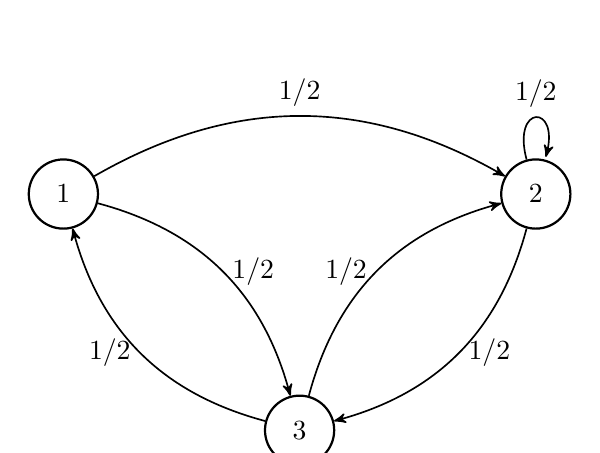
\begin{tikzpicture}[->, >=stealth', auto, semithick, node distance=3cm]
	\tikzstyle{every state}=[fill=white,draw=black,thick,text=black,scale=1]
	\node[state]    (1)                     {$1$};
	\node[]         (5)[right of=1]   {};
	\node[state]    (2)[right of=5]   {$2$};
	\node[]         (4)[below of=1]   {};
	\node[state]    (3)[right of =4]    {$3$};
	\path
	(1) edge[bend left,above]	node{$1/2$}	(2)
	(1) edge[bend left,right]	node{$1/2$}	(3)
	(2) edge[loop above]		node{$1/2$}	(2)
	(2) edge[bend left,right]	node{$1/2$}	(3)
	(3) edge[bend left,left]		node{$1/2$}	(1)
	(3) edge[bend left,left]		node{$1/2$}	(2);
	\end{tikzpicture}
\end{center}
I dette tilfælde er overgangsmatricen være givet ved
\begin{align*}
    \mathcal{P}=
\begin{bmatrix}
0 & \frac{1}{2} & \frac{1}{2}\\
0 & \frac{1}{2} & \frac{1}{2}\\
\frac{1}{2} & \frac{1}{2} & 0
\end{bmatrix},
\end{align*}
hvor $p_{ij}$ er den $ij$'te indgang. 
\end{eks}

Følgende sætning er en betingelse for, at en given sekvens af diskrete tilfældige variabler er en Markov-kæde.

\begin{minipage}\textwidth
\begin{thmx} \textbf{Markov betingelsen} \label{sæt:markov_tingtang}%Ny sætning
\newline 
Lad $\bm X=(X_0, X_1,\ldots)$ være en sekvens af diskrete tilfældige variabler med tilstandsrum, $S$ og lad $i_0, i_1, \ldots, i_t \in S$ være tilstande. Lad derudover $p_{ij}$ være overgangssandsynligheden. Så er $\bm X$ en Markov-kæde med overgangsmatricen, $\mathcal{P}$, hvis og kun hvis
\begin{align}
    P(X_0=i_0,X_1=i_1,\dots, X_t=i_t)=P(X_0=i_0)p_{i_0i_1}\dots p_{i_{t-1}i_t}\label{markov-kæde-hovedsætning}
\end{align}
for alle $t\geq0$ og $i_0,i_1,\dots,i_t\in S$. Begyndelsessandsynligheden er givet ved $P(X_0 = i_0)$.
\end{thmx}
\end{minipage}
\begin{bev} \textbf{}
\newline
Lad $\bm X = (X_0, X_1, \ldots)$ være en sekvens af diskrete tilfældige variabler og $i_0, i_1, \ldots, i_t \in S$ være tilstande. \\
Betegn $A_k = \{X_k = i_k\}$ og $\bm A_t=\bigcap_{k=0}^t A_k$. Hvis $P(\bm A_t)=0$, er beviset trivielt, og derfor antages det, at $P(\bm A_t)>0$ for alle $t$. 
Med ovenstående notation er \eqref{markov-kæde-hovedsætning} ækvivalent med følgende
\begin{align}\label{eq:omskrivning}
    %P(\{X_0=i_0\}\cap \{X_1=i_1\}\cap\dots\cap \{X_n=i_n\})=
    P(\bm A_t)=P(A_0)p_{i_0i_1}\cdots p_{i_{t-1}i_t}.
\end{align}
Dermed kan \eqref{markov-kæde-hovedsætning} bevises, ved at vise \eqref{eq:omskrivning}.

Først bevises det, at såfremt $\bm X$ er en Markov-kæde, så gælder \eqref{eq:omskrivning}. Dette gøres ved induktion.
Antag derfor, at $\bm X$ er en Markov-kæde med begyndelsesfordelingen $P(A_0)$ og overgangsmatricen $\P$. 

For $t=0$ gælder det, at $P(\bm A_0) = P(A_0) = P(X_0=i_0)$, og derved er induktionsstarten vist. Antag, at \eqref{eq:omskrivning} gælder for $t$. Det skal vises, at dette medfører, at \eqref{eq:omskrivning} er opfyldt for $t+1$. Af \autoref{def:betinget_sandsynlighed}, \eqref{eq:markov_egenskaben} og \autoref{def:overgangssandsynlighed} fås
%
\begin{align*}
     P(\bm A_{t+1}) = P(A_{t+1}\cap \bm A_{t})= P(\bm A_{t})P(A_{t+1}| A_t)=P(A_0)p_{i_0i_1}\dots p_{i_{t}i_{t+1}}
\end{align*}
Altså er induktionsskridtet vist. Det gælder dermed, at hvis $\bm X$ er en Markov-kæde, så er \eqref{eq:omskrivning} sand.  

Herefter vises det, at hvis \eqref{eq:omskrivning} gælder, så er Markov egenskaben, \eqref{eq:markov_egenskaben}, opfyldt. Antag derfor, at \eqref{eq:omskrivning} gælder for alle $t$ samt alle sekvenser $(i_m)$. Når $t = 0$, fås $P(\bm A_0)=P(A_0)$. Det følger af \autoref{def:betinget_sandsynlighed}, at
\begin{align*}
    P(A_{t+1}|\bm A_t)&=\frac{P(\bm A_{t+1})}{P(\bm A_t)}\\
    &= \frac{P(A_0)p_{i_0i_1}\cdots p_{i_{t-1}i_t}}{P(A_0)p_{i_0i_1}\cdots p_{i_{t-1}i_t}}\cdot p_{i_{t}i_{t+1}}
    \\
    &=p_{i_ni_{t+1}} = P(A_{t+1} | A_t).
\end{align*}
Altså er Markov egenskaben opfyldt, og $\bm X$ er en Markov-kæde med overgangsmatricen, $\P$. Dermed er \autoref{sæt:markov_tingtang} bevist. 

\end{bev}


\section{Tidsdynamik af Markov-kæder}
Hvis overgangssandsynligheden $p_{ij}$ er kendt, er det muligt at bestemme fremtidige overgangssandsynligheder. Overgangsmatricen består af $p_{ij}$, som er \textit{første trins overgangssandsynligheder}, hvor man generelt kan skrive \textit{t'te trins overgangssandsynligheder} som 
\begin{align}\label{eq:nte-trinsovergangssandsynligheden}
    p_{ij}^{(t)} = P ( X_t = j | X_0 = i).
\end{align}
Sandsynligheden for at gå fra tilstanden $i$ til $j$ efter $t$ trin er dermed givet ved $p_{ij}^{(t)}$. Ud fra $p_{ij}^{(t)}$ defineres $t$'te trins overgangsmatricen som $\P^{(t)}=\left[p_{ij}^{(t)}\right]$. Indgangene i matricen opfylder følgende

\begin{minipage}\textwidth
\begin{thmx} \textbf{Chapman-Kolmogorov ligningen}\label{sæt:chapman-kolmogrov} %Ny sætning
\newline
Lad $\bm X$ være en Markov-kæde med tilstandsrummet $S$ og lad $i,j, k \in S$ være tilstande. Lad derudover $p_{ij}^{(t)}$ være $t$'te trins overgangssandsynligheden. Da gælder det, at
\begin{align*}
    p_{ij}^{(t+m)} = \sum_{k \in S} p_{ik}^{(t)}p_{kj}^{(m)}
\end{align*}
for alle $t, m \geq 0$ og alle $i,j \in S$. 
\end{thmx}
\end{minipage}
\begin{bev} \textbf{} %Nyt bevis
\newline
Lad $\bm X$ være en Markov-kæde med tilstandsrummet $S$. Lad derudover $p_{ij}^{(t)}$ være $t$'te trins overgangssandsynligheden og lad $i,j, k \in S$ være tilstande. Eftersom Markov-kæden er homogen, og ved brug af loven om total sandsynlighed, \autoref{sæt:loven_om_total_sandsynlighed}, gælder det, at
\begin{align*}
    p_{ij}^{(t+m)} &= P(X_{t+m} = j | X_0 = i) = \sum_{k \in S} P (X_{t+m} = j | X_t = k, X_0 = i)P(X_t=k|X_0=i).
    \intertext{Af Markov egenskaben, \eqref{eq:markov_egenskaben}, fås dermed, at}
    p_{ij}^{(t+m)} &= \sum_{k \in S} P (X_{t+m} = j | X_t = k)P(X_t=k|X_0=i) \\ 
    &= \sum_{k \in S} p_{ik}^{(t)}p_{kj}^{(m)}.
\end{align*}
Dermed er \autoref{sæt:chapman-kolmogrov} bevist.
\end{bev}
Bemærk, at det følger af \autoref{sæt:chapman-kolmogrov}, at
\begin{align} \label{eq:chapman-kolmogorov}
    \P^{(t+m)} = \P^{(t)}\P^{(m)}
\end{align}
hvor $\P^{(t)}$ er $t$'te trins overgangsmatricen.
%hvor $\P^{(t)}$ og $\P^{(m)}$ er henholdsvis $t$'te trins og $m$'te trins overgangsmatricen

Hvis overgangsmatricen, $\P$, er kendt, er det muligt at bestemme $\P^{(t)}$ uden at skulle beregne $p_{ij}^{(t)}$.
Dette præsenteres i følgende sætning.

\begin{minipage}\textwidth
\begin{thmx}\textbf{Overgangsmatricen ved $\bm t$'te trin} \label{sæt:P(n)Pn} \\
Lad $\bm X$ være en Markov-kæde med tilstandsrummet, $S$. Lad $\P^{(t)}$ være $t$'te trins overgangsmatricen. Så gælder det, at
    \begin{align*}
        \P^{(t)} = \P^t.
    \end{align*}
\end{thmx}
\end{minipage}

\begin{bev}\textbf{}\\
Lad $\bm X = (X_0, X_1, \ldots)$ være en Markov-kæde med tilstandsrummet $S$ og $i,j\in S$ være tilstande. Lad $\P^{(t)}$ være $t$'te trins overgangsmatricen. For $t=1$ gælder det ud fra \autoref{def:overgangssandsynlighed}, at
\begin{align*}
    p_{ij}^{(1)} = P(X_1=j|X_0=i) = p_{ij}.
\end{align*}
Af \autoref{def:ovegangsmatrice} fås $\P^{(1)} = \left[p_{ij}^{(1)}\right] = \left[p_{ij}\right]= \P$. Ud fra \eqref{eq:chapman-kolmogorov} gælder det, at
\begin{align*}
    \P^{(t)}= \P^{(t-1)}\P^{(1)}=\prod_{k=1}^{t} \P^{(1)} = %P^{(1)}\cdots P^{(1)} = P^{1}\cdots P^1 = 
    \prod_{k=1}^{t} \P = \P^{t}.
\end{align*}
Dermed er \autoref{sæt:P(n)Pn} bevist.
\end{bev}


\section{Klassifikation af tilstande}

I dette afsnit præsenteres sammenhængen mellem tilstandsrummet, $S$, og overgangsmatricen, $\P$. Hvis overgangssandsynligheden mellem to tilstande er positiv, er det muligt at gå fra den ene tilstand til den anden. Dette præsenteres i følgende definition

\begin{minipage}\textwidth
\begin{defn}\textbf{Tilgængelighed} \label{def:tilgængelighed} %Ny definition
\newline
Lad $\bm X$ være en Markov-kæde med tilstandsrummet, $S$. Lad derudover $p_{ij}^{(t)}$ være $t$'te trins overgangssandsynligheden, og lad $i,j \in S$ være tilstande. Hvis der eksisterer et $t\in T$, hvorom der gælder, at $p_{ij}^{(t)}>0$, siges tilstanden, $j$, at være \textit{tilgængelig} fra tilstanden $i$. Dette noteres, $i\to j$. Hvis $i\to j$ og $j\to i$, siges det, at $i$ og $j$ \textit{kommunikerer}, hvilket noteres $i\leftrightarrow j$.
\end{defn}
\end{minipage}

Hvis der for en delmængde af $S$ gælder, at alle tilstande kommunikerer, kaldes delmængden en \textit{kommunikerende klasse}. Det er muligt, at alle tilstande i $S$ kommunikerer, hvilket fører til følgende definition 

\begin{minipage}\textwidth
\begin{defn}\label{def:ureducerbar} \textbf{Ureducerbar} %Ny definition
\newline
Lad $\bm X$ være en Markov-kæde med tilstandsrummet $S$. $\bm X$ siges at være \textit{ureducerbar}, hvis der for alle tilstande, $i,j \in S$ gælder, at $i \leftrightarrow j$.
\end{defn}
\end{minipage}

Ud over at det er muligt at bestemme om tilstande kommunikerer, kan det undersøges, hvorvidt det er muligt at komme tilbage til en tilstand. Heraf defineres følgende



\begin{minipage}\textwidth
\begin{defn}\textbf{Tilbagevendende og forbigående tilstande} \label{def:tau}%Ny definition
\newline
Lad $\bm X = (X_0, X_1, \dots)$ være en Markov-kæde med tilstandsrummet $S$. Lad derudover $i\in S$ være en tilstand og
\begin{align*}
    \tau_i=\min\{t\geq1:X_t=i\}.
\end{align*}
Hvis $P(\tau_i<\infty|X_0=i)=1$, siges tilstanden, $i$, at være \textit{tilbagevendende}. Hvis den ikke er tilbagevendende, siges den at være \textit{forbigående}.
\end{defn}
\end{minipage}

Altså er $\tau_i$ antallet af trin før kæden besøger $i$.

Hvis en tilstand er tilbagevendende, vil Markov-kæden med sikkerhed vende tilbage til tilstanden. Hvis tilstanden derimod er forbigående, vil der være en positiv sandsynlighed for, at Markov-kæden ikke vender tilbage til tilstanden. 

For at bestemme om en tilstand er tilbagevendende kan  følgende resultat anvendes.

\begin{minipage}\textwidth
\begin{thmx}\label{tilbagevendende} \textbf{Tilbagevendende tilstand} %Ny proposition
\newline
Lad $\bm X$ være en Markov-kæde med tilstandsrummet, $S$ og lad $i,j \in S$ være tilstande. Lad derudover $p_{ij}^{(t)}$ være $t$'te trins overgangssandsynligheden. Tilstanden $i$, er tilbagevendende, hvis
\begin{align*}
 \sum_{t=1}^\infty p_{ii}^{(t)}=\infty.
\end{align*}
\end{thmx}
\end{minipage}

\begin{bev} \textbf{} %Nyt bevis
\newline
Lad $\bm X = (X_0, X_1, \dots)$ være en Markov-kæde med tilstandsrummet $S$. Lad derudover $p_{ij}^{(t)}$ være $t$'te-trins overgangssandsynligheden og $i,j \in S$ være tilstande.

I dette bevis defineres indikatorfunktionen for alle $t \in \N$ som følgende
\begin{align*}
    I_t = 
  \begin{cases}
    1       & \quad \text{hvis } X_t = i\\
    0  & \quad \text{hvis } X_t \neq i
  \end{cases}
\end{align*}
Ud fra indikatorfunktionen, $I_t$, defineres antallet af gange Markov-kæden vender tilbage til tilstanden $i$, som 
\begin{align*}
    A = \sum_{t = 1}^{\infty} I_t.
\end{align*}
Det antages for modstrid, at Markov-kæden er forbigående, altså at $E\left[A | X_0 = i\right] < \infty$.

Det gælder, at
\begin{align}
    \infty > E\left[A | X_0 = i\right] &= \sum_{t=1}^{\infty} E\left[I_t | X_0 = i\right]. \label{lorte_eq}
    \intertext{Fra \autoref{def:betinget_forventet_værdi_af_diskrete_tilfældige_variabler} gælder det, at}
\sum_{t=1}^{\infty} E\left[I_t | X_0 = i\right] &= \sum_{t=1}^{\infty} \sum_{x \in \text{Range}(I_t)} xP\left(X_t=x | X_0 = i\right) = \sum_{t=1}^{\infty} P\left(X_t=i | X_0 = i\right). \nonumber
    \intertext{Af \eqref{eq:nte-trinsovergangssandsynligheden} følger det da, at}
    \sum_{t=1}^{\infty} P\left(X_t=i | X_0 = i \right) &= \sum_{t=1}^{\infty} p_{ii}^{(t)}.\nonumber
\end{align} 
Dette er en modstrid, da det er antages, at $\displaystyle \sum_{t=1}^{\infty} p_{ii}^{(t)} = \infty$. Altså må det gælde, at Markov-kæden er tilbagevendende, og dermed er \autoref{tilbagevendende} bevist. 

Det skal påpeges, at \eqref{lorte_eq} følger af Fubini-Tonelli's sætning, som ikke vil gennemgås i dette projekt. 
\end{bev}

For en ureducerbar Markov-kæde gælder følgende korollar

\begin{minipage}\textwidth
\begin{kor} \textbf{} \label{kor:enten_forbigå_eller_tilbagevend}%Nyt k
\newline
Lad $\bm X$ være en ureducerbar Markov-kæde. Så gælder det, at alle tilstande enten er forbigående eller tilbagevendende.
\end{kor}
\end{minipage}

\begin{bev} \textbf{} %Nyt bevis
\newline
Lad $\bm X$ være en Markovkæde med tilstandsrummet $S$. Lad derudover $p_{ij}^{(t)}$ være $t$'te-trins overgangssandsynligheden og $i,j \in S$ være tilstande.

Det bevises, at hvis én tilstand er tilbagevendende, medfører det, at alle tilstande er tilbagevendende. Altså skal alle tilstande enten være tilbagevendende eller forbigående. Fra \autoref{tilbagevendende} er det derved tilstrækkeligt at bevise, at %
\begin{align*}
    \sum_{t=1}^\infty p_{ii}^{(t)}=\infty \Leftrightarrow  \sum_{t=1}^\infty p_{jj}^{(t)}=\infty.
\end{align*}
%
Da Markov-kæden er ureducerbar, vil $i \leftrightarrow j$ for alle $i,j \in S$. Af \autoref{def:tilgængelighed} gælder det da, at $i \to j$ og $j \to i$, og dermed eksisterer der $t,m\geq 0$ således, at
\begin{align*}
    p_{ij}^{(t)} > 0 \quad \text{ og } \quad p_{ji}^{(m)} > 0.
\end{align*}
Altså
\begin{align*}
    \alpha = p_{ij}^{(t)}p_{ji}^{(m)} > 0.
\end{align*}
Det følger af \autoref{sæt:chapman-kolmogrov}, at
\begin{align*}
    p_{ii}^{(t+r+m)} = \sum_{j \in S} p_{ij}^{(t)} p_{jj}^{(r)}p_{ji}^{(m)} \geq p_{ij}^{(t)} p_{jj}^{(r)}p_{ji}^{(m)} = \alpha p_{jj}^{(r)} \text{ for } r \geq 0.
\end{align*}
Ved at summe over $r$ fås
\begin{align*}
    \sum_{r=0}^\infty p_{ii}^{(t+r+m)} \geq \alpha \sum_{r=0}^\infty p_{jj}^{(r)}.
\end{align*}
Deraf følger det, at hvis $\displaystyle\sum_{r=0}^\infty p_{jj}^{(r)}= \infty$, så er $\displaystyle\sum_{r=0}^\infty p_{ii}^{(t+r+m)} = \infty$. Hvis $\displaystyle\sum_{r=0}^\infty p_{ii}^{(t+r+m)} = \infty$, så følger det analogt, at $\displaystyle\sum_{r=0}^\infty p_{jj}^{(r)}= \infty$. Dermed er \autoref{kor:enten_forbigå_eller_tilbagevend} bevist.
\end{bev}

Det kan herved konkluderes, at hvis én tilstand er tilbagevendende eller forbigående i en ureducerbar Markov-kæde, så er alle tilstande dette.

I følgende eksempel, \autoref{eks:tilbage}, vil det blive vist, hvordan man undersøger, om en Markov-kæde er ureducerbar, og om tilstandene er forbigående eller tilbagevendende.

\begin{eks} \textbf{} \label{eks:tilbage}%Nyt eksempel
\newline
Lad $\bm X$ være en Markov-kæde givet som i \autoref{eks:overgangsmatrice}, hvor overgangsgrafen og overgangsmatricen blev bestemt. Først bestemmes det, om Markov-kæden er ureducerbar. Af \autoref{def:ureducerbar} følger det, at hvis alle tilstande i tilstandsrummet kommunikerer, er Markov-kæden ureducerbar. For at alle tilstande kommunikerer med hinanden, skal der eksistere et $t \in T$ således, at $p_{ij}^{(t)}>0$ for alle $i,j \in S$. Fra \autoref{eks:overgangsmatrice} er det givet, at en del af overgangssandsynlighederne er strengt positive, men da alle overgangssandsynlighederne skal være positive, undersøges overgangsmatricen for andet trin.
\begin{align*}
\mathcal{P}^2&=
\begin{bmatrix}
0 & \frac{1}{2} & \frac{1}{2}\\
0 & \frac{1}{2} & \frac{1}{2}\\
\frac{1}{2} & \frac{1}{2} & 0
\end{bmatrix}\begin{bmatrix}
0 & \frac{1}{2} & \frac{1}{2}\\
0 & \frac{1}{2} & \frac{1}{2}\\
\frac{1}{2} & \frac{1}{2} & 0
\end{bmatrix} =\begin{bmatrix}
\frac{1}{4} & \frac{1}{2} & \frac{1}{4}\\
\frac{1}{4} & \frac{1}{2} & \frac{1}{4}\\
 0 & \frac{1}{2} & \frac{1}{2}\\
\end{bmatrix}.
\intertext{Det gælder stadig ikke, at $p_{ij}^{(t)}>0$ for alle $i,j \in S$. Derfor bestemmes overgangsmatricen for tredje trin.}
\mathcal{P}^3&=
\begin{bmatrix}
\frac{1}{4} & \frac{1}{2} & \frac{1}{4}\\
\frac{1}{4} & \frac{1}{2} & \frac{1}{4}\\
 0 & \frac{1}{2} & \frac{1}{2}\\
\end{bmatrix}\begin{bmatrix}
0 & \frac{1}{2} & \frac{1}{2}\\
0 & \frac{1}{2} & \frac{1}{2}\\
\frac{1}{2} & \frac{1}{2} & 0
\end{bmatrix} =
\begin{bmatrix}
\frac{1}{8} & \frac{1}{2} & \frac{3}{8}\\
\frac{1}{8} & \frac{1}{2} & \frac{3}{8}\\
\frac{1}{4} & \frac{1}{2} & \frac{1}{4}\\
\end{bmatrix}.
\end{align*}
Da $p_{ij}^{(3)}>0$ for alle $i,j \in S$, følger det af \autoref{def:tilgængelighed}, at de tre tilstande er tilgængelige fra hinanden og dermed kommunikerer. Dermed gælder det jævnfør \autoref{def:ureducerbar}, at Markov-kæden er ureducerbar.

Herefter bestemmes det, om tilstandene i Markov-kæden er tilbagevendende eller forbigående. Af \autoref{kor:enten_forbigå_eller_tilbagevend} vides det, at alle tilstande i en ureducerbar kæde enten er forbigående eller tilbagevendende. Derfor undersøges det, om Markov-kæden har én tilbagevendende eller forbigående tilstand. Dette gøres ved at anvende \autoref{tilbagevendende}. Det er i Maple bestemt, hvad $t$'te trins overgangsandsynlighederne er givet ved. Ud fra dette gælder det, at
\begin{align*}
    \sum_{t=1}^\infty p_{22}^{(t)} = \sum_{t=1}^\infty \frac{1}{6} \cdot \left(3 \cdot (0^t +1)\right) = \infty
\end{align*}
Da $\displaystyle\sum_{t=1}^\infty p_{22}^{(t)}=\infty$, er tilstanden $2$ tilbagevendende, hvorved alle tilstandende i Markov-kæden er tilbagevendende. 
Dermed er det blevet bestemt, at Markov-kæden er ureducerbar og alle tilstandene er tilbagevendende.
\end{eks}

Hvis en tilstand i Markov-kæden er tilbagevendende, kan den enten være \textit{positiv-} eller \textit{null tilbagevendende}. Disse begreber defineres som følgende

\begin{defn}\textbf{Positiv og null tilbagevendende}\label{def:positiv_null_tilbagevendende} %Ny definition
\newline
Lad $\bm X$ være en Markov-kæde med tilstandsrummet, $S$, og $i\in S$ være en tilbagevendende tilstand.  Lad derudover  $\tau_i$ være antallet af trin før kæden besøger $i$. Hvis
\begin{enumerate}
    \item $E_i[\tau_i|X_0 = i]<\infty$, siges $i$ at være positiv tilbagevendende.
    \item $E_i[\tau_i|X_0 = i]=\infty$, siges $i$ at være null tilbagevendende.
\end{enumerate}
\end{defn}

Altså gælder det, at hvis $i$ er positiv tilbagevendende, forventes det, at Markov-kæden vender tilbage til tilstanden $i$ indenfor et endeligt antal trin. For en tilstand der er null tilbagevendende, forventes der derimod, at kæden ikke vender tilbage til tilstanden indenfor et endeligt antal trin. % der går uendeligt mange trin, før kæden vender tilbage til tilstanden. 

Ud over at tilstande kan klassificeres som forbigående, positiv tilbagevendende og null tilbagevendende, kan de også opdeles i \textit{aperiodiske} og \textit{periodiske} tilstande. Dette defineres som følgende

\begin{minipage}\textwidth
\begin{defn}\textbf{Perioden for en tilstand}\label{def:aperiodisk} %Ny definition
\newline
Lad $\bm X$ være en Markov-kæde med $t$'te trins overgangssandsynligheden $p_{ij}^{(t)}$, tilstandsrummet $S$ og tilstande $i,j \in S$. Perioden for $i$ er defineret som
\begin{align*}
    d(i) = gcd\{t\geq 1 : p_{ii}^{(t)}>0\}.
\end{align*}
Hvis $d(i)=1$, siges $i$ at være aperiodisk, ellers siges den at være periodisk.
\end{defn}
\end{minipage}

Altså er perioden defineret som den største fælles divisor af antallet af trin for at vende tilbage til $i$. Hvis en Markov-kæde for eksempel vender tilbage til tilstanden $i$ efter $3$ trin, men af en anden vej kan tage $6$ trin, vil den største fælles divisor være $3$. 

Hvis en Markov-kæde er ureducerbar og har én aperiodisk tilstand, gælder følgende lemma. 

%at alle tilstande i Markov-kæden er aperiodiske. Dette er præsenteret i følgende lemma


\begin{minipage}\textwidth
\begin{lem} \label{lem:lort}\textbf{} %Nyt lemma
\newline
Lad $\bm X$ være en ureducerbar Markov-kæde med tilstandsrummet $S$ og tilstande $i, j, k \in S$. Lad derudover $\bm X$ have $t$'te trins overgangssandsynligheden $p_{ij}^{(t)}$. Hvis $\bm X$ har en aperiodisk tilstand $k$, så gælder det, at der for alle tilstande $i$ og $j$, eksisterer et $N\in \N$ således, at $p_{ij}^{(t)}>0$ for alle $t\geq N$. 
\end{lem}
\end{minipage}

\begin{bev} \textbf{} %Nyt bevis
\newline
Lad $\bm X$ være en ureducerbar Markov-kæde med tilstandsrummet $S$ og tilstande $i, j, k \in S$. Lad derudover $\bm X$ have $t$'te trins overgangssandsynligheden $p_{ij}^{(t)}$ og $k$ være en aperiodisk tilstand.

Da $\bm X$ er ureducerbar, følger det af \autoref{def:tilgængelighed} og \autoref{def:ureducerbar}, at der eksisterer et $r, s\geq 0$ således, at overgangssandsynligheder, $p_{ik}^{(r)}, p_{kj}^{(s)}>0$. Da $k$ er aperiodisk, eksisterer der et $N\in \N$ således, at $p_{ij}^{(t)}>0$ for $t\geq N$. Dermed følger det af \autoref{sæt:chapman-kolmogrov}, at
\begin{align*}
    p_{ij}^{(r+t+s)}\geq p_{ik}^{(r)}p_{kk}^{(t)}p_{kj}^{(s)}>0
\end{align*}
Hermed er \autoref{lem:lort} bevist. 
\end{bev}

\section{Invariant fordeling}
Det er muligt at bestemme en Markov-kædes asymptotiske opførsel, når $\P$ er kendt. Dette gøres ved at bestemme $\displaystyle \lim_{t \to \infty} \P^{(t)}$. Hvis overgangssandsynlighederne konvergerer, er en mulig ligevægt for Markov-kæden den invariante fordeling. Den invariante fordeling defineres som følgende
%
\begin{defn}\textbf{Invariant fordeling} \label{defn: invariant_fordeling} %Ny definition
\newline 
Lad $\bm X$ være en Markov-kæde med tilstandsrummet, $S$, og overgangsmatricen, $\P$, lad derudover $i\in S$ være en tilstand. En sandsynlighedsfordeling, $\bm\pi=(\pi_i : i \in S)$, på $S$, som opfylder
\begin{enumerate}
    \item $\pi_i\geq 0 \text{ for } i\in S$,
    \item $\displaystyle\sum_{i\in S} \pi_i=1$,
    \item $\bm\pi \P=\bm\pi$,
\end{enumerate}
kaldes for en \textit{invariant fordeling} af kæden. 
\end{defn}
%Eftersom $S$ er endelig eller tællelig uendelig, er det muligt at definere sandsynlighedsfordelingen som en vektor $\bm {\pi} = (\pi_i: i \in S)$, hvor $\pi_i = p_X(i)$ er en frekvensfunktion over en tilfældig variabel $X$. 
Bemærk, at da $\bm X = (X_0, X_1, \ldots)$ er en Markov-kæde bestående af diskrete tilfældige variabler, er sandsynlighedsrummet endeligt eller tællelig uendeligt. Altså er det muligt at definere sandsynlighedsfordelingen som en vektor $\bm {\pi} = (\pi_i: i \in S)$, hvor $\pi_i = p_{X_t} (i)$ er en frekvensfunktion for en tilfældig variabel $X_t$. 

Den invariante fordeling er invariant i forhold til tiden, altså vil $\bm \pi \P^t = \bm\pi$ for $t = 1, 2, \ldots, N$. 

Derudover opfylder indgangene i $\bm \pi$, at
\begin{align}\label{eq:sum_invariant_fordeling}
     \pi_j=\sum_{i\in S}p_{ij}\pi_i \text{ for alle } j\in S. 
\end{align}

Der eksisterer ikke en invariant fordeling for enhver Markov-kæde, og hvis den eksisterer, er den ikke nødvendigvis entydig. 
Hvis Markov-kæden er ureducerbar, vil den invariante fordeling være entydig såfremt, at den eksisterer. Derudover er der en sammenhæng mellem positiv tilbagevendende tilstande og den invariante fordeling. Disse resultater præsenteres i følgende sætning

\begin{minipage}\textwidth
\begin{thmx} \label{sæt:den_vi_ikke_beviser}\textbf{Invariant fordeling og positiv tilbagevendende tilstande} %Ny sætning
\newline
Lad $\bm X$ være en ureducerbar Markov-kæde med tilstandsrummet, $S$ og tilstande $i, j\in S$. Lad derudover $\tau_i$ være antallet af trin før kæden besøger tilstanden $i$.
\begin{enumerate}
    \item Så eksisterer der en invariant fordeling, $\bm \pi$, hvis og kun hvis, der eksisterer en positiv tilbagevendende tilstand.
    \item Hvis der eksisterer en invariant fordeling $\bm \pi$, så er alle tilstande positiv tilbagevendende og
    \begin{align*}
        \pi_i = \frac{1}{E_i[\tau_i|X_0 = i]} \text{ for alle } i\in S. 
    \end{align*}
Altså er $\bm\pi$ entydig. 
\end{enumerate}
\end{thmx}
\end{minipage}

Denne sætning vil ikke blive bevist i dette projekt, men der henvises til \citep[s. 233-234]{oxford}. 

Af \autoref{sæt:den_vi_ikke_beviser} følger det dermed, at hvis der eksisterer en invariant fordeling for en ureducerbar Markov-kæde, så gælder det, at den er entydig, og alle tilstande er positiv tilbagevendende. Derudover medfører positiv tilbagevendende tilstande, at der eksisterer en invariant fordeling. 

\subsection{Konvergens mod den invariante fordeling}
I dette underafsnit vil resultatet om konvergens mod den invariante fordeling præsenteres. Dette beskriver, hvad en Markov-kæde skal opfylde, for at \textit{grænsefordelingen} er den invariante fordeling. Først defineres grænsefordelingen som følgende

%I dette underafsnit vil hovedresultatet være konvergens mod den invariante fordeling, som beskriver, hvad en Markov-kæde skal opfylde, for at grænsefordelingen er den invariante fordeling. Først defineres grænsefordelingen som følgende

\begin{minipage}\textwidth
\begin{defn}\textbf{Grænsefordeling} %Ny definition
\newline
Lad $\bm X$ være en ureducerbar Markov-kæde med tilstandsrummet, $S$ og tilstande $i, j\in S$. Lad derudover $\bm X$ have $t$'te trins overgangssandsynligheden $p_{ij}^{(t)}$. Såfremt der eksisterer en sandsynlighedsfordeling $\bm q$ på $S$ således, at
\begin{align*}
    p_{ij}^{(t)}\to q_j \text{ for } t\to \infty \text{ for alle } i,j\in S,
\end{align*}
kaldes $\bm q$ for Markov-kædens grænsefordeling. 
\end{defn}
\end{minipage}
%Altså gælder det, at hvis de asymptotiske sandsynligheder ikke afhænger af begyndelsestilstanden, $X_0=i$, kaldes fordelingen på det givne tilstandsrum en \textit{grænsefordeling}.


%Bemærk, at $\bm\pi$ er en rækkevektor med ikke-negative indgange. Sandsynligheden, $\pi_j$, fortæller altså, hvor lang tid der bruges i tilstand j i det lange løb. Derfor er det intuitivt, at der gælder følgende definition.

Følgende resultat præsenterer, hvornår den invariante fordeling er grænsefordelingen.

\begin{minipage}\textwidth
\begin{thmx} \textbf{Konvergens mod den invariante fordeling}\label{sæt:konvergens_for_markov} %Ny sætning
\newline
Lad $\bm X$ være en ureducerbar, aperiodisk og positiv tilbagevendende Markov-kæde med tilstandsrummet, $S$ og tilstande $i, j\in S$. Lad derudover $\bm X$ have $t$'te trins overgangssandsynligheden $p_{ij}^{(t)}$. Så gælder det, at 
\begin{align*}
    p_{ij}^{(t)} \to \pi_j \text{ for } t \to \infty,
\end{align*}
hvor $\bm \pi$ er Markov-kædens entydige invariante fordeling. 
\end{thmx}
\end{minipage}

For at kunne bevise \autoref{sæt:konvergens_for_markov} anvendes nogle hjælperesultater. Disse kan findes i \autoref{hjælpesæt}. 
\vspace{-0.4cm}
\begin{bev} \textbf{} %Nyt bevis
\newline
Lad $\bm X$ være en ureducerbar, aperiodisk og positiv tilbagevendende Markov-kæde med tilstandsrummet, $S$ og tilstande $i, j\in S$. Lad derudover $\bm X$ have $t$'te trins overgangssandsynligheden $p_{ij}^{(t)}$.

Lad $\bm Z = ( \bm X, \bm Y)$ være et ordnet par af uafhængige Markov-kæder, hvor $\bm X = (X_0, X_1, \ldots)$ og $\bm Y = (Y_0, Y_1, \ldots)$. 

Begge Markov-kæder har tilstandsrummet $S$ og overgangsmatrice $\P$. Deraf følger det, at $\bm Z = (Z_0, Z_1, \ldots)$ er en Markov-kæde med tilstandsrum $S \times S$, hvor $Z_t = (X_t, Y_t)$. Af \autoref{def:overgangssandsynlighed} er overgangssandsynlighederne for $\bm Z$ givet ved
\begin{align*}
    p_{ij, kl} &= P\left(Z_{t+1} = (k,l) | Z_t = (i,j)\right).
    \intertext{Da $\bm X$ og $\bm Y$ er uafhængige, følger det af \autoref{def:uafhængighed}, at}
    p_{ij, kl}&=P\left(X_{t+1} = k|X_t = i\right)P\left(Y_{t+1} = l|Y_t = j\right) = p_{ik}p_{jl}.
\end{align*}
Af \autoref{lem:lort} følger det, at for $i,j,k,l \in S$ eksisterer der et $N$ således, at $p_{ik}^{(t)}p_{jl}^{(t)}> 0$ for alle $t \geq N$. Altså eksisterer der ét $t$ således, at $p_{ij, kl}^{(t)}>0$, og $\bm Z$ er dermed ureducerbar som følge af \autoref{def:tilgængelighed} og \autoref{def:ureducerbar}. 

Da $\bm X$ er positiv tilbagevendende, har $\bm X$ en entydig invariant fordeling, $\bm \pi$, som følge af \autoref{sæt:den_vi_ikke_beviser} punkt 1. Dermed må der eksistere en positiv tilbagevendende tilstand i $\bm Z$, og af \autoref{sæt:den_vi_ikke_beviser} punkt 1 gælder det, at $\bm Z$ har en entydig invariante fordeling $\hat{\bm \pi} = (\hat{\pi}_{ij}:i,j\in S)$. Derfor er $\bm Z$ positiv tilbagevendende af \autoref{sæt:den_vi_ikke_beviser} punkt 2. Den invariante fordeling for $\bm Z$ er givet ved produktet mellem $\bm X$ og $\bm Y$'s invariante fordelinger, da $\bm X$ og $\bm Y$ er uafhængige. Derudover har $\bm X$ og $\bm Y$ den samme sandsynlighedsfordeling og dermed også samme invariante fordeling. Den invariante fordeling for $\bm Z$ er altså givet ved $\hat{\pi}_{ij} = \pi_i\pi_j$. %Derfor er $\bm Z$ positiv tilbagevendende af \autoref{sæt:den_vi_ikke_beviser} punkt 2. 

Lad $X_0=i$ og $Y_0=j$ således, at $Z_0=(i,j)$. Lad derudover $s\in S$ være en tilstand sådan at
\begin{align*}
    \tau=\min\{t\geq 1:Z_t=(s,s)\},
\end{align*}
er antallet af trin før kæden besøger $(s,s)$. Altså det mindste antal af trin før Markov-kæderne $\bm X$ og $\bm Y$ er lig hinanden. Da $\bm Z$ er positiv tilbagevendende følger det af \autoref{def:tau}, at
\begin{align}\label{tauss}
    P\left(\tau < \infty |Z_0 = (i, j)\right) = 1.
\end{align}
Altså er $\tau$ endelig. Det skal vises, at grænsefordelingen for $\bm X$ og $\bm Y$ er uafhængige af deres begyndelsesandsynlighed.
\begin{align*}
    p_{ik}^{(t)}&=P\left(X_t=k | Z_0 = (i,j)\right).
    \intertext{Da $\{\tau \leq t\}$ og $\{\tau > t\}$ er disjunkte hændelser, følger det af \autoref{def:sandsynlighedsregningens_grundsætninger} punkt 3, at}
    p_{ik}^{(t)}&=P\left(X_t=k, \tau\leq t | Z_0 = (i,j)\right)+P\left(X_t=k, \tau> t | Z_0 = (i,j)\right).
    \intertext{Af den stærke Markov egenskab (se \autoref{stærk_markov}), med $\tau$ som stoptid (se \autoref{stoptid}), gælder det, at $X_n$ og $Y_n$ har den samme betingede sandsynlighed givet, at $\{\tau \leq n\}$}
    p_{ik}^{(t)}&=P\left(Y_t=k, \tau\leq t| Z_0 = (i,j)\right)+P\left(X_t=k, \tau> t| Z_0 = (i,j)\right)\\
    &\leq P\left(Y_t=k| Z_0 = (i,j)\right)+P\left(\tau> t| Z_0=(i,j)\right)\\
    &= p_{jk}^{(t)} + P\left(\tau> t| Z_0 = (i,j)\right)
\end{align*}
Ud fra ovenstående og \eqref{tauss} fås følgende
\begin{align*}
    \left|p_{ik}^{(t)} - p_{jk}^{(t)}\right| \leq P\left(\tau> t| Z_0 = (i,j)\right) \to 0 \text{ for } t \to \infty
\end{align*}
Dette medfører, at
\begin{align*}
    p_{ik}^{(t)} - p_{jk}^{(t)} \to 0 \text{ for } t \to \infty.
\end{align*}
Hvis grænsen $\displaystyle \lim_{t \to \infty} p_{ik}^{(t)}$ eksisterer, afhænger den dermed ikke af $i$. 

Herefter vises det, at grænsen eksisterer. Fra \eqref{eq:sum_invariant_fordeling} og \autoref{defn: invariant_fordeling} punkt 2 følger det, at
\begin{align*}
    \pi_k-p_{jk}^{(t)}&=%\sum_{i\in S}\pi_ip_{ik}^{(t)}-p_{jk}^{(t)}\\
    \sum_{i\in S} p_{ik}^{(t)} \pi_i - \sum_{i\in S} \pi_i p_{jk}^{(t)}=\sum_{i\in S}\pi_i\left(p_{ik}^{(t)}-p_{jk}^{(t)}\right) 
\end{align*}
Da $ p_{ik}^{(t)} - p_{jk}^{(t)} \to 0$ for $t\to \infty$, følger det af \autoref{sidstelemma}, at $\displaystyle\sum_{i\in S}\pi_i\left(p_{ik}^{(t)}-p_{jk}^{(t)}\right)\to 0 $ for $ t \to \infty$.
Altså gælder det, at $p_{ij}^{(t)} \to \pi_j \text{ for } t \to \infty$, og dermed er \autoref{sæt:konvergens_for_markov} bevist.
\end{bev}

Det vil i følgende eksempel, \autoref{eks:invariant}, blive vist, hvordan man undersøger, om en Markov-kæde har en invariant fordeling. Derudover vil den invariante fordeling blive bestemt, og til sidst vil det konkluderes, om Markov-kæden har den invariante fordeling som grænsefordeling.

\begin{eks}\textbf{}\label{eks:invariant}\\
Lad $\bm X = (X_0, X_1, \ldots)$ være en Markov-kæde givet som i \autoref{eks:overgangsmatrice}. Det vil først bestemmes, om denne Markov-kæde har en invariant fordeling. Af \autoref{sæt:den_vi_ikke_beviser} gælder det, at hvis Markov-kæden har en positiv tilbagevendende tilstand, så er alle tilstandene positiv tilbagevendende, og der eksisterer en entydig invariant fordeling. Fra \autoref{eks:tilbage} er det bestemt, at Markov-kæden er ureducerbar, og at alle tilstandene er tilbagevendende. Derfor undersøges det, om en af tilstandene er positiv tilbagevendende. Dette gøres ud fra \autoref{def:positiv_null_tilbagevendende}.
\begin{align*}
    E_2[\tau_2| X_0 = 2]&=\sum_{k\in \N} kP(\tau_2=k|X_0=2)\\
    &=\frac{1}{2} + \left(\frac{1}{2}\right)^2 + \left(\frac{1}{2}\right)^3 + \left(\frac{1}{2}\right)^4 + \ldots\\
    &= \sum_{k \in \N} \left(\frac{1}{2}\right)^k = 1
\end{align*}
Da $ E_2[\tau_2 | X_0 = 2]<\infty$, følger det af \autoref{def:positiv_null_tilbagevendende}, at tilstanden, $2$, er positiv tilbagevendende, hvorved alle tilstandene i Markov-kæden er positiv tilbagevendende, og derfor eksisterer der en entydig invariant fordeling.

Ud fra \autoref{defn: invariant_fordeling} skal den invariante fordeling opfylde, at 
\begin{align*}
    \begin{bmatrix}
    \pi_1 & \pi_2 & \pi_3
    \end{bmatrix}
    \begin{bmatrix}
    0 & \frac{1}{2} & \frac{1}{2}\\
    0 & \frac{1}{2} & \frac{1}{2}\\
    \frac{1}{2} & \frac{1}{2} & 0
    \end{bmatrix} &= \begin{bmatrix}
    \pi_1 & \pi_2 & \pi_3
    \end{bmatrix}.
    \intertext{Dette opstilles som tre ligninger med tre ubekendte.}
    \frac{1}{2}\pi_3 &=\pi_1,\\
    \frac{1}{2}\pi_1 + \frac{1}{2} \pi_2+ \frac{1}{2}\pi_3 &=\pi_2, \\
    \frac{1}{2}\pi_1 + \frac{1}{2} \pi_2 &= \pi_3.
    \intertext{Dermed skal det gælde, at}
    \pi_3 = 2\pi_1 \text{ og } \pi_2 &= 3\pi_1
\end{align*}
Af \autoref{defn: invariant_fordeling} skal det være opfyldt, at $\displaystyle \sum_{i \in S} \pi_i = 1$, og dermed er den invariante fordeling givet ved følgende
\begin{align*}
    \bm \pi = \begin{bmatrix}
    \frac{1}{6} & \frac{1}{2} & \frac{1}{3}
    \end{bmatrix}.
\end{align*}

Til sidst vil det blive bestemt, om Markov-kæden har den invariante fordeling som grænsefordeling. For at undersøge om Markov-kæden konvergerer mod den invariante fordeling, skal det jævnfør \autoref{sæt:konvergens_for_markov} også gælde, at den er aperiodisk. Da der for $t=3$ gælder, at $p_{ij}^{(t)} > 0$ for alle $i,j \in S$, er alle tilstande i tilstandsrummet aperiodiske. Da Markov-kæden er ureducerbar, aperiodisk og positiv tilbagevendende, følger det af \autoref{sæt:konvergens_for_markov}, at den konvergerer mod den invariante fordeling. 
\end{eks}




\chapter{Forbrugsproblemet}
En investor ønsker at maksimere sin \textit{nytte} over en given periode.
Lad tidshorisonten være givet ved $T$. Investorens opsparing til tiden $t$ betegnes ved $S_t$, sådan at $S_0$ er givet. Investoren kan enten forbruge eller lade pengene akkumulere til en rente, $r$. Lad $A_t$ være forbrug og indkomst være $I>0$. I dette afsnit konstrueres en MDP over disse beslutninger, med henblik på maksimering af nytte. Følgende tabel opsummerer disse variabler.


\begin{table}[!hbt]
\caption{Variabler for investeringsproblemet}
\begin{tabular}{@{}l|l@{}}
\toprule
Variabler & Forklaring                     \\ \midrule
$T,t$       & Tidspunkter                  \\
$S_t$       & Opsparing til tiden t        \\
$r$         & Rente                        \\
$A_t$       & Forbrug                      \\
$I$         & Indkomst                     \\
$\xi_t$     & $\begin{cases}1\ \text{Hvis i arbejde}\\0\ \text{Ellers}\end{cases}$ \\ \bottomrule
\end{tabular}
\end{table}




Opsparing til tiden $t+1$ er dermed givet ved
\begin{align*}
    S_{t+1}=(1+r)(S_t-A_t)+I\dot \xi_t
\end{align*}


\section{Basis Problemet}


\begin{align*}
    P(\xi_{t+1}=0|\xi_t=1)=1-P(\xi_{t+1}=1|\xi_t=1)=p\\
    P(\xi_{t+1}=0|\xi_t=0)=1-P(\xi_{t+1}=1|\xi_t=0)=q
\end{align*}

\begin{align*}
    \mathcal{A}_t=[0,S_t]
\end{align*}

\begin{align*}
    E^\pi[\sum_{t=1}^T U_t(A_t)]
\end{align*}




%\pagebreak

\section{Udvidet problem}
I det udvidede problem undersøges det, hvordan muligheden for at optage lån påvirker forbrugerens forventede maksimale belønning og forbrug. Det antages, at forbrugeren er fornuftig, og dermed er belønningsfunktionen \eqref{eq:belønning_fornuftig_forbruger}. Derudover er sandsynligheden for, at forbrugeren er i arbejde beskrevet ved Markov-kæden med overgangssandsynlighederne, \eqref{eq:markov_kæde_problem}.

Da der i denne udvidelse antages, at forbrugeren har muligheden for at optage lån, afhænger den fremtidige opsparing også af lånet og udlånsrenten. Altså er den fremtidige opsparing givet ved
\begin{align*} 
    S_{t+1} =(1 + \gamma_i)(S_t-a_t - L_t \cdot \gamma_u) + \xi_t \cdot I,
\end{align*}
hvor $\gamma_i$ betegner indlånsrenten, $\gamma_u$ udlånsrenten og $L_t$ det samlede lån frem til beslutningstidspunkt $t$. Altså afdrager forbrugeren renterne på lånet, før han modtager afkast fra banken. 
%  V[N][s, xi, L_N] = R(s - L_N * (1 + udlånsrente))    
Det antages desuden, at der forbruges, hvad der lånes i det pågældende beslutningstidspunkt, og at lånet tilbagebetales i beslutningstidspunkt $t=N$.

Lad $L$ betegne lånebegrænsningen, som er det maksimale beløb, forbrugeren kan låne til hvert beslutningstidspunkt. Da det er muligt for forbrugeren at låne til hvert beslutningstidspunkt, er beslutningsrummet givet ved
\begin{align*}
    A_t(S_t) = [0, S_t] \times [0, L].
\end{align*}
%
Det antages, at forbrugeren ikke må have gæld efter det sidste beslutningstidspunkt, og dermed skal hele lånet og de tilhørende udlånsrenter være tilbagebetalt ved sidste beslutningstidspunkt. Altså gælder det, at
\begin{align*}
    L_N \leq S_N.
\end{align*}
Ud fra ovenstående vil det analyseres, hvordan forbruget samt den forventede maksimale belønning påvirkes af varierende lånebegrænsninger, renter og sandsynligheder for arbejdsløshed. For at kunne analysere dette vil disse faktorer varieres, mens nedenstående faktorer fastholdes til følgende værdier, medmindre andet er angivet
\begin{align}\label{fastevariable}
    \begin{split}
        N=11,\\
        S_0 = 100,\\
        I=10,\\
        \Delta = 1,\\
        \alpha = 0.1, \\
        \beta = 0.5,\\
        L = 2.\
    \end{split}
\end{align}

\subsection[Variation af  \texorpdfstring{$\gamma_i$ og $\gamma_u$}{Variation af indlåns- og udlånsrenten}]{Variation af \bm{$\gamma_i$} og \bm{$\gamma_u$}}
Først undersøges det, hvordan forbruget og den forventede maksimale belønning påvirkes, når indlåns- og udlånsrenten er ækvivalente. Derfor fastholdes de andre faktorer som i \eqref{fastevariable}.

Værdierne for indlåns- og udlånsrenten der sammenlignes, er henholdsvis $\gamma_i = \gamma_u= 0.01, \gamma_i = \gamma_u=0.02$ og $\gamma_i = \gamma_u=0.05$.

Ved at anvende de ovenstående værdier i den implementerede algoritme, \autoref{Bilag:python_kode}, bestemmes den optimale strategi, inklusiv lån, for forbrugeren samt den forventede maksimale belønning givet denne strategi. Disse værdier er præsenteret i nedenstående tabel, \autoref{tab:ind_ud_ens}.

\begin{table}[H]
\captionsetup{font=large}
\centering
\resizebox{10cm}{!}{%
\begin{tabular}{|c|ccc|}   \hline
 $\gamma_i=\gamma_u$      & 0.01 & 0.02  & 0.05 \\ \thickhline
 $t$    &   &   Forbrug & \\ \hline
0   & 16.00(0) & 15.00(0) & 14.00(0)   \\ \hline
1   & 15.91(0) & 14.90(0) & 13.9(0) \\  \hline
2   & 15.77(0) & 15.64(0) & 14.43(0)   \\ \hline 
3   & 15.62(0) & 15.43(0) & 14.48(0)   \\ \hline 
4   & 15.57(0) & 15.17(0) & 15.22(0.17)  \\  \hline 
5   & 16.13(0) & 15.71(0.01) & 15.55(0.08)  \\    \hline 
6   & 15.97(0) & 15.86(0.27) & 15.09(1.4)  \\ \hline 
7   & 16.33(0) & 16.37(1.37) & 20.66(0.37)   \\ \hline 
8   & 16.18(0) & 19.08(0) & 23.16(1.24)    \\ \hline 
9   & 16.52(0) & 19.58(0) & 26.58(0.56)  \\   \hline 
10  & 16.89(0) & 19.95(0) & 28.86(0.25)  \\ \hline 
11  & 17.46(0) & 20.88(0) & 31.52(0)   \\   \thickhline
 Belønning & 48.28 & 49.33& 52.41        \\ \thickhline
\end{tabular}
}
\caption{Optimal strategi samt belønning ved variation af $\gamma_i = \gamma_u$.}\label{tab:ind_ud_ens}
\end{table}

I ovenstående tabel er de optimale strategier samt den tilhørende forventede maksimale belønning præsenteret i kolonne 2-4. Derudover er beslutningstidspunkterne angivet i kolonne 1. Til hvert beslutningstidspunkt kan det optimale forbrug aflæses, hvor tallene i parenteserne repræsenterer den andel af forbruget, som lånet udgør. De optimale strategier, samt lånet, illustreres i nedenstående figur, \autoref{fig:lån_i=u}, hvor figuren til venstre repræsenterer forbruget, inklusiv lån, og figuren til højre repræsenterer lånet. 

\begin{figure}[H] 
    \begin{center}
        \resizebox{8cm}{!}{\input{Afsnit/PGF/i=u_samlet.pgf}}
        \resizebox{8cm}{!}{%% Creator: Matplotlib, PGF backend
%%
%% To include the figure in your LaTeX document, write
%%   \input{<filename>.pgf}
%%
%% Make sure the required packages are loaded in your preamble
%%   \usepackage{pgf}
%%
%% Figures using additional raster images can only be included by \input if
%% they are in the same directory as the main LaTeX file. For loading figures
%% from other directories you can use the `import` package
%%   \usepackage{import}
%%
%% and then include the figures with
%%   \import{<path to file>}{<filename>.pgf}
%%
%% Matplotlib used the following preamble
%%
\begingroup%
\makeatletter%
\begin{pgfpicture}%
\pgfpathrectangle{\pgfpointorigin}{\pgfqpoint{6.400000in}{4.800000in}}%
\pgfusepath{use as bounding box, clip}%
\begin{pgfscope}%
\pgfsetbuttcap%
\pgfsetmiterjoin%
\definecolor{currentfill}{rgb}{1.000000,1.000000,1.000000}%
\pgfsetfillcolor{currentfill}%
\pgfsetlinewidth{0.000000pt}%
\definecolor{currentstroke}{rgb}{1.000000,1.000000,1.000000}%
\pgfsetstrokecolor{currentstroke}%
\pgfsetdash{}{0pt}%
\pgfpathmoveto{\pgfqpoint{0.000000in}{0.000000in}}%
\pgfpathlineto{\pgfqpoint{6.400000in}{0.000000in}}%
\pgfpathlineto{\pgfqpoint{6.400000in}{4.800000in}}%
\pgfpathlineto{\pgfqpoint{0.000000in}{4.800000in}}%
\pgfpathclose%
\pgfusepath{fill}%
\end{pgfscope}%
\begin{pgfscope}%
\pgfsetbuttcap%
\pgfsetmiterjoin%
\definecolor{currentfill}{rgb}{1.000000,1.000000,1.000000}%
\pgfsetfillcolor{currentfill}%
\pgfsetlinewidth{0.000000pt}%
\definecolor{currentstroke}{rgb}{0.000000,0.000000,0.000000}%
\pgfsetstrokecolor{currentstroke}%
\pgfsetstrokeopacity{0.000000}%
\pgfsetdash{}{0pt}%
\pgfpathmoveto{\pgfqpoint{0.800000in}{0.528000in}}%
\pgfpathlineto{\pgfqpoint{5.760000in}{0.528000in}}%
\pgfpathlineto{\pgfqpoint{5.760000in}{4.224000in}}%
\pgfpathlineto{\pgfqpoint{0.800000in}{4.224000in}}%
\pgfpathclose%
\pgfusepath{fill}%
\end{pgfscope}%
\begin{pgfscope}%
\pgfsetbuttcap%
\pgfsetroundjoin%
\definecolor{currentfill}{rgb}{0.000000,0.000000,0.000000}%
\pgfsetfillcolor{currentfill}%
\pgfsetlinewidth{0.803000pt}%
\definecolor{currentstroke}{rgb}{0.000000,0.000000,0.000000}%
\pgfsetstrokecolor{currentstroke}%
\pgfsetdash{}{0pt}%
\pgfsys@defobject{currentmarker}{\pgfqpoint{0.000000in}{-0.048611in}}{\pgfqpoint{0.000000in}{0.000000in}}{%
\pgfpathmoveto{\pgfqpoint{0.000000in}{0.000000in}}%
\pgfpathlineto{\pgfqpoint{0.000000in}{-0.048611in}}%
\pgfusepath{stroke,fill}%
}%
\begin{pgfscope}%
\pgfsys@transformshift{1.025455in}{0.528000in}%
\pgfsys@useobject{currentmarker}{}%
\end{pgfscope}%
\end{pgfscope}%
\begin{pgfscope}%
\definecolor{textcolor}{rgb}{0.000000,0.000000,0.000000}%
\pgfsetstrokecolor{textcolor}%
\pgfsetfillcolor{textcolor}%
\pgftext[x=1.025455in,y=0.430778in,,top]{\color{textcolor}\rmfamily\fontsize{10.000000}{12.000000}\selectfont \(\displaystyle {0}\)}%
\end{pgfscope}%
\begin{pgfscope}%
\pgfsetbuttcap%
\pgfsetroundjoin%
\definecolor{currentfill}{rgb}{0.000000,0.000000,0.000000}%
\pgfsetfillcolor{currentfill}%
\pgfsetlinewidth{0.803000pt}%
\definecolor{currentstroke}{rgb}{0.000000,0.000000,0.000000}%
\pgfsetstrokecolor{currentstroke}%
\pgfsetdash{}{0pt}%
\pgfsys@defobject{currentmarker}{\pgfqpoint{0.000000in}{-0.048611in}}{\pgfqpoint{0.000000in}{0.000000in}}{%
\pgfpathmoveto{\pgfqpoint{0.000000in}{0.000000in}}%
\pgfpathlineto{\pgfqpoint{0.000000in}{-0.048611in}}%
\pgfusepath{stroke,fill}%
}%
\begin{pgfscope}%
\pgfsys@transformshift{1.845289in}{0.528000in}%
\pgfsys@useobject{currentmarker}{}%
\end{pgfscope}%
\end{pgfscope}%
\begin{pgfscope}%
\definecolor{textcolor}{rgb}{0.000000,0.000000,0.000000}%
\pgfsetstrokecolor{textcolor}%
\pgfsetfillcolor{textcolor}%
\pgftext[x=1.845289in,y=0.430778in,,top]{\color{textcolor}\rmfamily\fontsize{10.000000}{12.000000}\selectfont \(\displaystyle {2}\)}%
\end{pgfscope}%
\begin{pgfscope}%
\pgfsetbuttcap%
\pgfsetroundjoin%
\definecolor{currentfill}{rgb}{0.000000,0.000000,0.000000}%
\pgfsetfillcolor{currentfill}%
\pgfsetlinewidth{0.803000pt}%
\definecolor{currentstroke}{rgb}{0.000000,0.000000,0.000000}%
\pgfsetstrokecolor{currentstroke}%
\pgfsetdash{}{0pt}%
\pgfsys@defobject{currentmarker}{\pgfqpoint{0.000000in}{-0.048611in}}{\pgfqpoint{0.000000in}{0.000000in}}{%
\pgfpathmoveto{\pgfqpoint{0.000000in}{0.000000in}}%
\pgfpathlineto{\pgfqpoint{0.000000in}{-0.048611in}}%
\pgfusepath{stroke,fill}%
}%
\begin{pgfscope}%
\pgfsys@transformshift{2.665124in}{0.528000in}%
\pgfsys@useobject{currentmarker}{}%
\end{pgfscope}%
\end{pgfscope}%
\begin{pgfscope}%
\definecolor{textcolor}{rgb}{0.000000,0.000000,0.000000}%
\pgfsetstrokecolor{textcolor}%
\pgfsetfillcolor{textcolor}%
\pgftext[x=2.665124in,y=0.430778in,,top]{\color{textcolor}\rmfamily\fontsize{10.000000}{12.000000}\selectfont \(\displaystyle {4}\)}%
\end{pgfscope}%
\begin{pgfscope}%
\pgfsetbuttcap%
\pgfsetroundjoin%
\definecolor{currentfill}{rgb}{0.000000,0.000000,0.000000}%
\pgfsetfillcolor{currentfill}%
\pgfsetlinewidth{0.803000pt}%
\definecolor{currentstroke}{rgb}{0.000000,0.000000,0.000000}%
\pgfsetstrokecolor{currentstroke}%
\pgfsetdash{}{0pt}%
\pgfsys@defobject{currentmarker}{\pgfqpoint{0.000000in}{-0.048611in}}{\pgfqpoint{0.000000in}{0.000000in}}{%
\pgfpathmoveto{\pgfqpoint{0.000000in}{0.000000in}}%
\pgfpathlineto{\pgfqpoint{0.000000in}{-0.048611in}}%
\pgfusepath{stroke,fill}%
}%
\begin{pgfscope}%
\pgfsys@transformshift{3.484959in}{0.528000in}%
\pgfsys@useobject{currentmarker}{}%
\end{pgfscope}%
\end{pgfscope}%
\begin{pgfscope}%
\definecolor{textcolor}{rgb}{0.000000,0.000000,0.000000}%
\pgfsetstrokecolor{textcolor}%
\pgfsetfillcolor{textcolor}%
\pgftext[x=3.484959in,y=0.430778in,,top]{\color{textcolor}\rmfamily\fontsize{10.000000}{12.000000}\selectfont \(\displaystyle {6}\)}%
\end{pgfscope}%
\begin{pgfscope}%
\pgfsetbuttcap%
\pgfsetroundjoin%
\definecolor{currentfill}{rgb}{0.000000,0.000000,0.000000}%
\pgfsetfillcolor{currentfill}%
\pgfsetlinewidth{0.803000pt}%
\definecolor{currentstroke}{rgb}{0.000000,0.000000,0.000000}%
\pgfsetstrokecolor{currentstroke}%
\pgfsetdash{}{0pt}%
\pgfsys@defobject{currentmarker}{\pgfqpoint{0.000000in}{-0.048611in}}{\pgfqpoint{0.000000in}{0.000000in}}{%
\pgfpathmoveto{\pgfqpoint{0.000000in}{0.000000in}}%
\pgfpathlineto{\pgfqpoint{0.000000in}{-0.048611in}}%
\pgfusepath{stroke,fill}%
}%
\begin{pgfscope}%
\pgfsys@transformshift{4.304793in}{0.528000in}%
\pgfsys@useobject{currentmarker}{}%
\end{pgfscope}%
\end{pgfscope}%
\begin{pgfscope}%
\definecolor{textcolor}{rgb}{0.000000,0.000000,0.000000}%
\pgfsetstrokecolor{textcolor}%
\pgfsetfillcolor{textcolor}%
\pgftext[x=4.304793in,y=0.430778in,,top]{\color{textcolor}\rmfamily\fontsize{10.000000}{12.000000}\selectfont \(\displaystyle {8}\)}%
\end{pgfscope}%
\begin{pgfscope}%
\pgfsetbuttcap%
\pgfsetroundjoin%
\definecolor{currentfill}{rgb}{0.000000,0.000000,0.000000}%
\pgfsetfillcolor{currentfill}%
\pgfsetlinewidth{0.803000pt}%
\definecolor{currentstroke}{rgb}{0.000000,0.000000,0.000000}%
\pgfsetstrokecolor{currentstroke}%
\pgfsetdash{}{0pt}%
\pgfsys@defobject{currentmarker}{\pgfqpoint{0.000000in}{-0.048611in}}{\pgfqpoint{0.000000in}{0.000000in}}{%
\pgfpathmoveto{\pgfqpoint{0.000000in}{0.000000in}}%
\pgfpathlineto{\pgfqpoint{0.000000in}{-0.048611in}}%
\pgfusepath{stroke,fill}%
}%
\begin{pgfscope}%
\pgfsys@transformshift{5.124628in}{0.528000in}%
\pgfsys@useobject{currentmarker}{}%
\end{pgfscope}%
\end{pgfscope}%
\begin{pgfscope}%
\definecolor{textcolor}{rgb}{0.000000,0.000000,0.000000}%
\pgfsetstrokecolor{textcolor}%
\pgfsetfillcolor{textcolor}%
\pgftext[x=5.124628in,y=0.430778in,,top]{\color{textcolor}\rmfamily\fontsize{10.000000}{12.000000}\selectfont \(\displaystyle {10}\)}%
\end{pgfscope}%
\begin{pgfscope}%
\definecolor{textcolor}{rgb}{0.000000,0.000000,0.000000}%
\pgfsetstrokecolor{textcolor}%
\pgfsetfillcolor{textcolor}%
\pgftext[x=3.280000in,y=0.251766in,,top]{\color{textcolor}\rmfamily\fontsize{10.000000}{12.000000}\selectfont \(\displaystyle t\)}%
\end{pgfscope}%
\begin{pgfscope}%
\pgfsetbuttcap%
\pgfsetroundjoin%
\definecolor{currentfill}{rgb}{0.000000,0.000000,0.000000}%
\pgfsetfillcolor{currentfill}%
\pgfsetlinewidth{0.803000pt}%
\definecolor{currentstroke}{rgb}{0.000000,0.000000,0.000000}%
\pgfsetstrokecolor{currentstroke}%
\pgfsetdash{}{0pt}%
\pgfsys@defobject{currentmarker}{\pgfqpoint{-0.048611in}{0.000000in}}{\pgfqpoint{-0.000000in}{0.000000in}}{%
\pgfpathmoveto{\pgfqpoint{-0.000000in}{0.000000in}}%
\pgfpathlineto{\pgfqpoint{-0.048611in}{0.000000in}}%
\pgfusepath{stroke,fill}%
}%
\begin{pgfscope}%
\pgfsys@transformshift{0.800000in}{0.696000in}%
\pgfsys@useobject{currentmarker}{}%
\end{pgfscope}%
\end{pgfscope}%
\begin{pgfscope}%
\definecolor{textcolor}{rgb}{0.000000,0.000000,0.000000}%
\pgfsetstrokecolor{textcolor}%
\pgfsetfillcolor{textcolor}%
\pgftext[x=0.525308in, y=0.647775in, left, base]{\color{textcolor}\rmfamily\fontsize{10.000000}{12.000000}\selectfont \(\displaystyle {0.0}\)}%
\end{pgfscope}%
\begin{pgfscope}%
\pgfsetbuttcap%
\pgfsetroundjoin%
\definecolor{currentfill}{rgb}{0.000000,0.000000,0.000000}%
\pgfsetfillcolor{currentfill}%
\pgfsetlinewidth{0.803000pt}%
\definecolor{currentstroke}{rgb}{0.000000,0.000000,0.000000}%
\pgfsetstrokecolor{currentstroke}%
\pgfsetdash{}{0pt}%
\pgfsys@defobject{currentmarker}{\pgfqpoint{-0.048611in}{0.000000in}}{\pgfqpoint{-0.000000in}{0.000000in}}{%
\pgfpathmoveto{\pgfqpoint{-0.000000in}{0.000000in}}%
\pgfpathlineto{\pgfqpoint{-0.048611in}{0.000000in}}%
\pgfusepath{stroke,fill}%
}%
\begin{pgfscope}%
\pgfsys@transformshift{0.800000in}{1.172934in}%
\pgfsys@useobject{currentmarker}{}%
\end{pgfscope}%
\end{pgfscope}%
\begin{pgfscope}%
\definecolor{textcolor}{rgb}{0.000000,0.000000,0.000000}%
\pgfsetstrokecolor{textcolor}%
\pgfsetfillcolor{textcolor}%
\pgftext[x=0.525308in, y=1.124709in, left, base]{\color{textcolor}\rmfamily\fontsize{10.000000}{12.000000}\selectfont \(\displaystyle {0.2}\)}%
\end{pgfscope}%
\begin{pgfscope}%
\pgfsetbuttcap%
\pgfsetroundjoin%
\definecolor{currentfill}{rgb}{0.000000,0.000000,0.000000}%
\pgfsetfillcolor{currentfill}%
\pgfsetlinewidth{0.803000pt}%
\definecolor{currentstroke}{rgb}{0.000000,0.000000,0.000000}%
\pgfsetstrokecolor{currentstroke}%
\pgfsetdash{}{0pt}%
\pgfsys@defobject{currentmarker}{\pgfqpoint{-0.048611in}{0.000000in}}{\pgfqpoint{-0.000000in}{0.000000in}}{%
\pgfpathmoveto{\pgfqpoint{-0.000000in}{0.000000in}}%
\pgfpathlineto{\pgfqpoint{-0.048611in}{0.000000in}}%
\pgfusepath{stroke,fill}%
}%
\begin{pgfscope}%
\pgfsys@transformshift{0.800000in}{1.649868in}%
\pgfsys@useobject{currentmarker}{}%
\end{pgfscope}%
\end{pgfscope}%
\begin{pgfscope}%
\definecolor{textcolor}{rgb}{0.000000,0.000000,0.000000}%
\pgfsetstrokecolor{textcolor}%
\pgfsetfillcolor{textcolor}%
\pgftext[x=0.525308in, y=1.601643in, left, base]{\color{textcolor}\rmfamily\fontsize{10.000000}{12.000000}\selectfont \(\displaystyle {0.4}\)}%
\end{pgfscope}%
\begin{pgfscope}%
\pgfsetbuttcap%
\pgfsetroundjoin%
\definecolor{currentfill}{rgb}{0.000000,0.000000,0.000000}%
\pgfsetfillcolor{currentfill}%
\pgfsetlinewidth{0.803000pt}%
\definecolor{currentstroke}{rgb}{0.000000,0.000000,0.000000}%
\pgfsetstrokecolor{currentstroke}%
\pgfsetdash{}{0pt}%
\pgfsys@defobject{currentmarker}{\pgfqpoint{-0.048611in}{0.000000in}}{\pgfqpoint{-0.000000in}{0.000000in}}{%
\pgfpathmoveto{\pgfqpoint{-0.000000in}{0.000000in}}%
\pgfpathlineto{\pgfqpoint{-0.048611in}{0.000000in}}%
\pgfusepath{stroke,fill}%
}%
\begin{pgfscope}%
\pgfsys@transformshift{0.800000in}{2.126802in}%
\pgfsys@useobject{currentmarker}{}%
\end{pgfscope}%
\end{pgfscope}%
\begin{pgfscope}%
\definecolor{textcolor}{rgb}{0.000000,0.000000,0.000000}%
\pgfsetstrokecolor{textcolor}%
\pgfsetfillcolor{textcolor}%
\pgftext[x=0.525308in, y=2.078577in, left, base]{\color{textcolor}\rmfamily\fontsize{10.000000}{12.000000}\selectfont \(\displaystyle {0.6}\)}%
\end{pgfscope}%
\begin{pgfscope}%
\pgfsetbuttcap%
\pgfsetroundjoin%
\definecolor{currentfill}{rgb}{0.000000,0.000000,0.000000}%
\pgfsetfillcolor{currentfill}%
\pgfsetlinewidth{0.803000pt}%
\definecolor{currentstroke}{rgb}{0.000000,0.000000,0.000000}%
\pgfsetstrokecolor{currentstroke}%
\pgfsetdash{}{0pt}%
\pgfsys@defobject{currentmarker}{\pgfqpoint{-0.048611in}{0.000000in}}{\pgfqpoint{-0.000000in}{0.000000in}}{%
\pgfpathmoveto{\pgfqpoint{-0.000000in}{0.000000in}}%
\pgfpathlineto{\pgfqpoint{-0.048611in}{0.000000in}}%
\pgfusepath{stroke,fill}%
}%
\begin{pgfscope}%
\pgfsys@transformshift{0.800000in}{2.603736in}%
\pgfsys@useobject{currentmarker}{}%
\end{pgfscope}%
\end{pgfscope}%
\begin{pgfscope}%
\definecolor{textcolor}{rgb}{0.000000,0.000000,0.000000}%
\pgfsetstrokecolor{textcolor}%
\pgfsetfillcolor{textcolor}%
\pgftext[x=0.525308in, y=2.555511in, left, base]{\color{textcolor}\rmfamily\fontsize{10.000000}{12.000000}\selectfont \(\displaystyle {0.8}\)}%
\end{pgfscope}%
\begin{pgfscope}%
\pgfsetbuttcap%
\pgfsetroundjoin%
\definecolor{currentfill}{rgb}{0.000000,0.000000,0.000000}%
\pgfsetfillcolor{currentfill}%
\pgfsetlinewidth{0.803000pt}%
\definecolor{currentstroke}{rgb}{0.000000,0.000000,0.000000}%
\pgfsetstrokecolor{currentstroke}%
\pgfsetdash{}{0pt}%
\pgfsys@defobject{currentmarker}{\pgfqpoint{-0.048611in}{0.000000in}}{\pgfqpoint{-0.000000in}{0.000000in}}{%
\pgfpathmoveto{\pgfqpoint{-0.000000in}{0.000000in}}%
\pgfpathlineto{\pgfqpoint{-0.048611in}{0.000000in}}%
\pgfusepath{stroke,fill}%
}%
\begin{pgfscope}%
\pgfsys@transformshift{0.800000in}{3.080670in}%
\pgfsys@useobject{currentmarker}{}%
\end{pgfscope}%
\end{pgfscope}%
\begin{pgfscope}%
\definecolor{textcolor}{rgb}{0.000000,0.000000,0.000000}%
\pgfsetstrokecolor{textcolor}%
\pgfsetfillcolor{textcolor}%
\pgftext[x=0.525308in, y=3.032445in, left, base]{\color{textcolor}\rmfamily\fontsize{10.000000}{12.000000}\selectfont \(\displaystyle {1.0}\)}%
\end{pgfscope}%
\begin{pgfscope}%
\pgfsetbuttcap%
\pgfsetroundjoin%
\definecolor{currentfill}{rgb}{0.000000,0.000000,0.000000}%
\pgfsetfillcolor{currentfill}%
\pgfsetlinewidth{0.803000pt}%
\definecolor{currentstroke}{rgb}{0.000000,0.000000,0.000000}%
\pgfsetstrokecolor{currentstroke}%
\pgfsetdash{}{0pt}%
\pgfsys@defobject{currentmarker}{\pgfqpoint{-0.048611in}{0.000000in}}{\pgfqpoint{-0.000000in}{0.000000in}}{%
\pgfpathmoveto{\pgfqpoint{-0.000000in}{0.000000in}}%
\pgfpathlineto{\pgfqpoint{-0.048611in}{0.000000in}}%
\pgfusepath{stroke,fill}%
}%
\begin{pgfscope}%
\pgfsys@transformshift{0.800000in}{3.557604in}%
\pgfsys@useobject{currentmarker}{}%
\end{pgfscope}%
\end{pgfscope}%
\begin{pgfscope}%
\definecolor{textcolor}{rgb}{0.000000,0.000000,0.000000}%
\pgfsetstrokecolor{textcolor}%
\pgfsetfillcolor{textcolor}%
\pgftext[x=0.525308in, y=3.509379in, left, base]{\color{textcolor}\rmfamily\fontsize{10.000000}{12.000000}\selectfont \(\displaystyle {1.2}\)}%
\end{pgfscope}%
\begin{pgfscope}%
\pgfsetbuttcap%
\pgfsetroundjoin%
\definecolor{currentfill}{rgb}{0.000000,0.000000,0.000000}%
\pgfsetfillcolor{currentfill}%
\pgfsetlinewidth{0.803000pt}%
\definecolor{currentstroke}{rgb}{0.000000,0.000000,0.000000}%
\pgfsetstrokecolor{currentstroke}%
\pgfsetdash{}{0pt}%
\pgfsys@defobject{currentmarker}{\pgfqpoint{-0.048611in}{0.000000in}}{\pgfqpoint{-0.000000in}{0.000000in}}{%
\pgfpathmoveto{\pgfqpoint{-0.000000in}{0.000000in}}%
\pgfpathlineto{\pgfqpoint{-0.048611in}{0.000000in}}%
\pgfusepath{stroke,fill}%
}%
\begin{pgfscope}%
\pgfsys@transformshift{0.800000in}{4.034538in}%
\pgfsys@useobject{currentmarker}{}%
\end{pgfscope}%
\end{pgfscope}%
\begin{pgfscope}%
\definecolor{textcolor}{rgb}{0.000000,0.000000,0.000000}%
\pgfsetstrokecolor{textcolor}%
\pgfsetfillcolor{textcolor}%
\pgftext[x=0.525308in, y=3.986313in, left, base]{\color{textcolor}\rmfamily\fontsize{10.000000}{12.000000}\selectfont \(\displaystyle {1.4}\)}%
\end{pgfscope}%
\begin{pgfscope}%
\definecolor{textcolor}{rgb}{0.000000,0.000000,0.000000}%
\pgfsetstrokecolor{textcolor}%
\pgfsetfillcolor{textcolor}%
\pgftext[x=0.469752in,y=2.376000in,,bottom,rotate=90.000000]{\color{textcolor}\rmfamily\fontsize{10.000000}{12.000000}\selectfont Lån}%
\end{pgfscope}%
\begin{pgfscope}%
\pgfpathrectangle{\pgfqpoint{0.800000in}{0.528000in}}{\pgfqpoint{4.960000in}{3.696000in}}%
\pgfusepath{clip}%
\pgfsetrectcap%
\pgfsetroundjoin%
\pgfsetlinewidth{1.505625pt}%
\definecolor{currentstroke}{rgb}{0.121569,0.466667,0.705882}%
\pgfsetstrokecolor{currentstroke}%
\pgfsetdash{}{0pt}%
\pgfpathmoveto{\pgfqpoint{1.025455in}{0.696000in}}%
\pgfpathlineto{\pgfqpoint{1.435372in}{0.696000in}}%
\pgfpathlineto{\pgfqpoint{1.845289in}{0.696000in}}%
\pgfpathlineto{\pgfqpoint{2.255207in}{0.696000in}}%
\pgfpathlineto{\pgfqpoint{2.665124in}{0.696000in}}%
\pgfpathlineto{\pgfqpoint{3.075041in}{0.696000in}}%
\pgfpathlineto{\pgfqpoint{3.484959in}{0.696000in}}%
\pgfpathlineto{\pgfqpoint{3.894876in}{0.696000in}}%
\pgfpathlineto{\pgfqpoint{4.304793in}{0.696000in}}%
\pgfpathlineto{\pgfqpoint{4.714711in}{0.696000in}}%
\pgfpathlineto{\pgfqpoint{5.124628in}{0.696000in}}%
\pgfpathlineto{\pgfqpoint{5.534545in}{0.696000in}}%
\pgfusepath{stroke}%
\end{pgfscope}%
\begin{pgfscope}%
\pgfpathrectangle{\pgfqpoint{0.800000in}{0.528000in}}{\pgfqpoint{4.960000in}{3.696000in}}%
\pgfusepath{clip}%
\pgfsetrectcap%
\pgfsetroundjoin%
\pgfsetlinewidth{1.505625pt}%
\definecolor{currentstroke}{rgb}{1.000000,0.498039,0.054902}%
\pgfsetstrokecolor{currentstroke}%
\pgfsetdash{}{0pt}%
\pgfpathmoveto{\pgfqpoint{1.025455in}{0.696000in}}%
\pgfpathlineto{\pgfqpoint{1.435372in}{0.696000in}}%
\pgfpathlineto{\pgfqpoint{1.845289in}{0.696000in}}%
\pgfpathlineto{\pgfqpoint{2.255207in}{0.696000in}}%
\pgfpathlineto{\pgfqpoint{2.665124in}{0.696000in}}%
\pgfpathlineto{\pgfqpoint{3.075041in}{0.726524in}}%
\pgfpathlineto{\pgfqpoint{3.484959in}{1.330322in}}%
\pgfpathlineto{\pgfqpoint{3.894876in}{3.962521in}}%
\pgfpathlineto{\pgfqpoint{4.304793in}{0.696000in}}%
\pgfpathlineto{\pgfqpoint{4.714711in}{0.696000in}}%
\pgfpathlineto{\pgfqpoint{5.124628in}{0.696000in}}%
\pgfpathlineto{\pgfqpoint{5.534545in}{0.696000in}}%
\pgfusepath{stroke}%
\end{pgfscope}%
\begin{pgfscope}%
\pgfpathrectangle{\pgfqpoint{0.800000in}{0.528000in}}{\pgfqpoint{4.960000in}{3.696000in}}%
\pgfusepath{clip}%
\pgfsetrectcap%
\pgfsetroundjoin%
\pgfsetlinewidth{1.505625pt}%
\definecolor{currentstroke}{rgb}{0.172549,0.627451,0.172549}%
\pgfsetstrokecolor{currentstroke}%
\pgfsetdash{}{0pt}%
\pgfpathmoveto{\pgfqpoint{1.025455in}{0.696000in}}%
\pgfpathlineto{\pgfqpoint{1.435372in}{0.696000in}}%
\pgfpathlineto{\pgfqpoint{1.845289in}{0.696000in}}%
\pgfpathlineto{\pgfqpoint{2.255207in}{0.696000in}}%
\pgfpathlineto{\pgfqpoint{2.665124in}{1.095194in}}%
\pgfpathlineto{\pgfqpoint{3.075041in}{0.895358in}}%
\pgfpathlineto{\pgfqpoint{3.484959in}{4.056000in}}%
\pgfpathlineto{\pgfqpoint{3.894876in}{1.578805in}}%
\pgfpathlineto{\pgfqpoint{4.304793in}{3.654899in}}%
\pgfpathlineto{\pgfqpoint{4.714711in}{2.027123in}}%
\pgfpathlineto{\pgfqpoint{5.124628in}{1.291214in}}%
\pgfpathlineto{\pgfqpoint{5.534545in}{0.696000in}}%
\pgfusepath{stroke}%
\end{pgfscope}%
\begin{pgfscope}%
\pgfsetrectcap%
\pgfsetmiterjoin%
\pgfsetlinewidth{0.803000pt}%
\definecolor{currentstroke}{rgb}{0.000000,0.000000,0.000000}%
\pgfsetstrokecolor{currentstroke}%
\pgfsetdash{}{0pt}%
\pgfpathmoveto{\pgfqpoint{0.800000in}{0.528000in}}%
\pgfpathlineto{\pgfqpoint{0.800000in}{4.224000in}}%
\pgfusepath{stroke}%
\end{pgfscope}%
\begin{pgfscope}%
\pgfsetrectcap%
\pgfsetmiterjoin%
\pgfsetlinewidth{0.803000pt}%
\definecolor{currentstroke}{rgb}{0.000000,0.000000,0.000000}%
\pgfsetstrokecolor{currentstroke}%
\pgfsetdash{}{0pt}%
\pgfpathmoveto{\pgfqpoint{5.760000in}{0.528000in}}%
\pgfpathlineto{\pgfqpoint{5.760000in}{4.224000in}}%
\pgfusepath{stroke}%
\end{pgfscope}%
\begin{pgfscope}%
\pgfsetrectcap%
\pgfsetmiterjoin%
\pgfsetlinewidth{0.803000pt}%
\definecolor{currentstroke}{rgb}{0.000000,0.000000,0.000000}%
\pgfsetstrokecolor{currentstroke}%
\pgfsetdash{}{0pt}%
\pgfpathmoveto{\pgfqpoint{0.800000in}{0.528000in}}%
\pgfpathlineto{\pgfqpoint{5.760000in}{0.528000in}}%
\pgfusepath{stroke}%
\end{pgfscope}%
\begin{pgfscope}%
\pgfsetrectcap%
\pgfsetmiterjoin%
\pgfsetlinewidth{0.803000pt}%
\definecolor{currentstroke}{rgb}{0.000000,0.000000,0.000000}%
\pgfsetstrokecolor{currentstroke}%
\pgfsetdash{}{0pt}%
\pgfpathmoveto{\pgfqpoint{0.800000in}{4.224000in}}%
\pgfpathlineto{\pgfqpoint{5.760000in}{4.224000in}}%
\pgfusepath{stroke}%
\end{pgfscope}%
\begin{pgfscope}%
\pgfsetbuttcap%
\pgfsetmiterjoin%
\definecolor{currentfill}{rgb}{1.000000,1.000000,1.000000}%
\pgfsetfillcolor{currentfill}%
\pgfsetfillopacity{0.800000}%
\pgfsetlinewidth{1.003750pt}%
\definecolor{currentstroke}{rgb}{0.800000,0.800000,0.800000}%
\pgfsetstrokecolor{currentstroke}%
\pgfsetstrokeopacity{0.800000}%
\pgfsetdash{}{0pt}%
\pgfpathmoveto{\pgfqpoint{0.916667in}{3.393445in}}%
\pgfpathlineto{\pgfqpoint{2.470889in}{3.393445in}}%
\pgfpathquadraticcurveto{\pgfqpoint{2.504223in}{3.393445in}}{\pgfqpoint{2.504223in}{3.426779in}}%
\pgfpathlineto{\pgfqpoint{2.504223in}{4.107333in}}%
\pgfpathquadraticcurveto{\pgfqpoint{2.504223in}{4.140667in}}{\pgfqpoint{2.470889in}{4.140667in}}%
\pgfpathlineto{\pgfqpoint{0.916667in}{4.140667in}}%
\pgfpathquadraticcurveto{\pgfqpoint{0.883333in}{4.140667in}}{\pgfqpoint{0.883333in}{4.107333in}}%
\pgfpathlineto{\pgfqpoint{0.883333in}{3.426779in}}%
\pgfpathquadraticcurveto{\pgfqpoint{0.883333in}{3.393445in}}{\pgfqpoint{0.916667in}{3.393445in}}%
\pgfpathclose%
\pgfusepath{stroke,fill}%
\end{pgfscope}%
\begin{pgfscope}%
\pgfsetrectcap%
\pgfsetroundjoin%
\pgfsetlinewidth{1.505625pt}%
\definecolor{currentstroke}{rgb}{0.121569,0.466667,0.705882}%
\pgfsetstrokecolor{currentstroke}%
\pgfsetdash{}{0pt}%
\pgfpathmoveto{\pgfqpoint{0.950000in}{4.015667in}}%
\pgfpathlineto{\pgfqpoint{1.283333in}{4.015667in}}%
\pgfusepath{stroke}%
\end{pgfscope}%
\begin{pgfscope}%
\definecolor{textcolor}{rgb}{0.000000,0.000000,0.000000}%
\pgfsetstrokecolor{textcolor}%
\pgfsetfillcolor{textcolor}%
\pgftext[x=1.416667in,y=3.957333in,left,base]{\color{textcolor}\rmfamily\fontsize{12.000000}{14.400000}\selectfont \(\displaystyle \gamma_i = \gamma_u = 0.01\)}%
\end{pgfscope}%
\begin{pgfscope}%
\pgfsetrectcap%
\pgfsetroundjoin%
\pgfsetlinewidth{1.505625pt}%
\definecolor{currentstroke}{rgb}{1.000000,0.498039,0.054902}%
\pgfsetstrokecolor{currentstroke}%
\pgfsetdash{}{0pt}%
\pgfpathmoveto{\pgfqpoint{0.950000in}{3.783260in}}%
\pgfpathlineto{\pgfqpoint{1.283333in}{3.783260in}}%
\pgfusepath{stroke}%
\end{pgfscope}%
\begin{pgfscope}%
\definecolor{textcolor}{rgb}{0.000000,0.000000,0.000000}%
\pgfsetstrokecolor{textcolor}%
\pgfsetfillcolor{textcolor}%
\pgftext[x=1.416667in,y=3.724926in,left,base]{\color{textcolor}\rmfamily\fontsize{12.000000}{14.400000}\selectfont \(\displaystyle \gamma_i = \gamma_u = 0.02\)}%
\end{pgfscope}%
\begin{pgfscope}%
\pgfsetrectcap%
\pgfsetroundjoin%
\pgfsetlinewidth{1.505625pt}%
\definecolor{currentstroke}{rgb}{0.172549,0.627451,0.172549}%
\pgfsetstrokecolor{currentstroke}%
\pgfsetdash{}{0pt}%
\pgfpathmoveto{\pgfqpoint{0.950000in}{3.550853in}}%
\pgfpathlineto{\pgfqpoint{1.283333in}{3.550853in}}%
\pgfusepath{stroke}%
\end{pgfscope}%
\begin{pgfscope}%
\definecolor{textcolor}{rgb}{0.000000,0.000000,0.000000}%
\pgfsetstrokecolor{textcolor}%
\pgfsetfillcolor{textcolor}%
\pgftext[x=1.416667in,y=3.492519in,left,base]{\color{textcolor}\rmfamily\fontsize{12.000000}{14.400000}\selectfont \(\displaystyle \gamma_i = \gamma_u = 0.05\)}%
\end{pgfscope}%
\end{pgfpicture}%
\makeatother%
\endgroup%
}
    \end{center}
    \caption{Forbrug af henholdsvis opsparing og lån med variation af $\gamma_u=\gamma_i$}\label{fig:lån_i=u}
\end{figure}
På samme måde som i basis-problemet kan det i \autoref{tab:ind_ud_ens} og \autoref{fig:lån_i=u} aflæses, at den forventede maksimale belønning stiger, når indlånsrenten stiger. Desuden bemærkes det, at den forventede maksimale belønning er omtrent den samme som i basis-problemet givet samme indlånsrenter, som i \autoref{tab:ændring_r}. Altså kan det ligesom ved basis-problemet aflæses, at hældningen på kurverne er større ved højere indlånsrenter, hvilket igen illustrerer, at forbrugeren udnytter renters renter mere og dermed fordeler sit forbrug mindre ligeligt mellem månederne.

%I \autoref{tab:ind_ud_ens} og \autoref{fig:lån_i=u} kan det aflæses, at den maksimale belønning stiger i takt med, at indlånsrenten stiger på samme måde som i basisproblemet. Desuden bemærkes det, at belønningen er omtrent den samme som i basisproblemet. 

Da $\Delta = 1$, kan der kun forbruges nærmeste heltal. Derfor er der små afrundingsfejl, som resulterer i, at forbrugeren i nogle beslutningstidspunkter har en præference til at låne. Disse lån har ingen betydning, da den forventede maksimale belønning er uafhængig af lån, når indlåns- og udlånsrenten er den samme. 

%Grunden til, at investoren vælger at låne ved større rente er uvis, men det postuleres, at det har noget at gøre med Delta. 

Herefter vil det analyseres, hvordan forbruget påvirkes, når $\gamma_i \neq \gamma_u$. Det forventes, at når udlånsrenten er større end indlånsrenten, vil forbrugeren undlade at låne. 
Denne forventning er baseret på, at lånet vil vokse hurtigere end opsparingen, hvilket resulterer i et negativt afkast. Omvendt forventes det, at forbrugeren får en højere forventet maksimal belønning ved at låne, når udlånsrenten er lavere end indlånsrenten.

Først analyseres tilfældet, hvor $\gamma_i < \gamma_u$. Indlånsrenten fastholdes til $0.01$, mens alle andre faktorer fastholdes med værdierne givet i \eqref{fastevariable}.

Udlånsrenten vil henholdsvis være $\gamma_u = 0.02, \gamma_u = 0.03$ og $\gamma_u = 0.04$. Ved at anvende disse værdier for $\gamma_u$ i den implementerede algoritme, \autoref{Bilag:python_kode}, bestemmes den optimale strategi, inklusiv lån, for forbrugeren samt den forventede maksimale belønning givet denne strategi. Disse værdier er præsenteret i nedenstående tabel, \autoref{tab:ind_udvari}.

\begin{table}[H]
\captionsetup{font=large}
\centering
\resizebox{11cm}{!}{%
\begin{tabular}{|c|ccc|}   \hline
 $\gamma_i$   & 0.01 & 0.01 & 0.01\\ 
 $\gamma_u$      & 0.02 & 0.03  & 0.04 \\\thickhline
  $t$    &   & Forbrug & \\ \hline
 0    & 16.00(0) & 16.00(0) & 16.00(0)  \\ \hline
 1    & 15.90(0) & 15.90(0) & 15.89(0)\\  \hline
 2    & 15.76(0) & 15.76(0)  & 15.76(0) \\ \hline 
 3    & 15.60(0) & 15.61(0)  & 15.60(0)\\ \hline 
 4    & 15.56(0) & 15.56(0)  & 15.56(0)\\  \hline 
 5    & 16.13(0) & 16.12(0) & 16.11(0) \\    \hline 
 6    & 15.98(0) & 15.98(0) & 15.95(0) \\ \hline 
 7    & 16.37(0) & 16.37(0)  & 16.34(0) \\   \hline 
 8    & 16.21(0) & 16.22(0)  & 16.20(0) \\ \hline 
 9    & 16.57(0) & 16.59(0)& 16.59(0)  \\   \hline 
 10   & 16.95(0) & 17.00(0) & 17.01(0) \\ \hline 
 11   & 17.52(0) & 17.59(0) &  17.58(0) \\   \thickhline
 Belønning & 48.31& 48.33  & 48.32 \\ \thickhline
\end{tabular}
}
\caption{Optimal strategi samt belønning ved variation af $ \gamma_u$.}\label{tab:ind_udvari}
\end{table}

%%
Forbruget og lånet kan aflæses i ovenstående tabel på samme måde som i \autoref{tab:ind_ud_ens}. 
De optimale strategier, samt lånet, illustreres i nedenstående figur, \autoref{fig:lån_gamma_u}, hvor figuren til venstre repræsenterer forbruget, inklusiv lån, og figuren til højre repræsenterer lånet. 
%
% 
\begin{figure}[H]
    \begin{center}
        \resizebox{8cm}{!}{%% Creator: Matplotlib, PGF backend
%%
%% To include the figure in your LaTeX document, write
%%   \input{<filename>.pgf}
%%
%% Make sure the required packages are loaded in your preamble
%%   \usepackage{pgf}
%%
%% Figures using additional raster images can only be included by \input if
%% they are in the same directory as the main LaTeX file. For loading figures
%% from other directories you can use the `import` package
%%   \usepackage{import}
%%
%% and then include the figures with
%%   \import{<path to file>}{<filename>.pgf}
%%
%% Matplotlib used the following preamble
%%
\begingroup%
\makeatletter%
\begin{pgfpicture}%
\pgfpathrectangle{\pgfpointorigin}{\pgfqpoint{6.400000in}{4.800000in}}%
\pgfusepath{use as bounding box, clip}%
\begin{pgfscope}%
\pgfsetbuttcap%
\pgfsetmiterjoin%
\definecolor{currentfill}{rgb}{1.000000,1.000000,1.000000}%
\pgfsetfillcolor{currentfill}%
\pgfsetlinewidth{0.000000pt}%
\definecolor{currentstroke}{rgb}{1.000000,1.000000,1.000000}%
\pgfsetstrokecolor{currentstroke}%
\pgfsetdash{}{0pt}%
\pgfpathmoveto{\pgfqpoint{0.000000in}{0.000000in}}%
\pgfpathlineto{\pgfqpoint{6.400000in}{0.000000in}}%
\pgfpathlineto{\pgfqpoint{6.400000in}{4.800000in}}%
\pgfpathlineto{\pgfqpoint{0.000000in}{4.800000in}}%
\pgfpathclose%
\pgfusepath{fill}%
\end{pgfscope}%
\begin{pgfscope}%
\pgfsetbuttcap%
\pgfsetmiterjoin%
\definecolor{currentfill}{rgb}{1.000000,1.000000,1.000000}%
\pgfsetfillcolor{currentfill}%
\pgfsetlinewidth{0.000000pt}%
\definecolor{currentstroke}{rgb}{0.000000,0.000000,0.000000}%
\pgfsetstrokecolor{currentstroke}%
\pgfsetstrokeopacity{0.000000}%
\pgfsetdash{}{0pt}%
\pgfpathmoveto{\pgfqpoint{0.800000in}{0.528000in}}%
\pgfpathlineto{\pgfqpoint{5.760000in}{0.528000in}}%
\pgfpathlineto{\pgfqpoint{5.760000in}{4.224000in}}%
\pgfpathlineto{\pgfqpoint{0.800000in}{4.224000in}}%
\pgfpathclose%
\pgfusepath{fill}%
\end{pgfscope}%
\begin{pgfscope}%
\pgfsetbuttcap%
\pgfsetroundjoin%
\definecolor{currentfill}{rgb}{0.000000,0.000000,0.000000}%
\pgfsetfillcolor{currentfill}%
\pgfsetlinewidth{0.803000pt}%
\definecolor{currentstroke}{rgb}{0.000000,0.000000,0.000000}%
\pgfsetstrokecolor{currentstroke}%
\pgfsetdash{}{0pt}%
\pgfsys@defobject{currentmarker}{\pgfqpoint{0.000000in}{-0.048611in}}{\pgfqpoint{0.000000in}{0.000000in}}{%
\pgfpathmoveto{\pgfqpoint{0.000000in}{0.000000in}}%
\pgfpathlineto{\pgfqpoint{0.000000in}{-0.048611in}}%
\pgfusepath{stroke,fill}%
}%
\begin{pgfscope}%
\pgfsys@transformshift{1.025455in}{0.528000in}%
\pgfsys@useobject{currentmarker}{}%
\end{pgfscope}%
\end{pgfscope}%
\begin{pgfscope}%
\definecolor{textcolor}{rgb}{0.000000,0.000000,0.000000}%
\pgfsetstrokecolor{textcolor}%
\pgfsetfillcolor{textcolor}%
\pgftext[x=1.025455in,y=0.430778in,,top]{\color{textcolor}\rmfamily\fontsize{10.000000}{12.000000}\selectfont \(\displaystyle {0}\)}%
\end{pgfscope}%
\begin{pgfscope}%
\pgfsetbuttcap%
\pgfsetroundjoin%
\definecolor{currentfill}{rgb}{0.000000,0.000000,0.000000}%
\pgfsetfillcolor{currentfill}%
\pgfsetlinewidth{0.803000pt}%
\definecolor{currentstroke}{rgb}{0.000000,0.000000,0.000000}%
\pgfsetstrokecolor{currentstroke}%
\pgfsetdash{}{0pt}%
\pgfsys@defobject{currentmarker}{\pgfqpoint{0.000000in}{-0.048611in}}{\pgfqpoint{0.000000in}{0.000000in}}{%
\pgfpathmoveto{\pgfqpoint{0.000000in}{0.000000in}}%
\pgfpathlineto{\pgfqpoint{0.000000in}{-0.048611in}}%
\pgfusepath{stroke,fill}%
}%
\begin{pgfscope}%
\pgfsys@transformshift{1.845289in}{0.528000in}%
\pgfsys@useobject{currentmarker}{}%
\end{pgfscope}%
\end{pgfscope}%
\begin{pgfscope}%
\definecolor{textcolor}{rgb}{0.000000,0.000000,0.000000}%
\pgfsetstrokecolor{textcolor}%
\pgfsetfillcolor{textcolor}%
\pgftext[x=1.845289in,y=0.430778in,,top]{\color{textcolor}\rmfamily\fontsize{10.000000}{12.000000}\selectfont \(\displaystyle {2}\)}%
\end{pgfscope}%
\begin{pgfscope}%
\pgfsetbuttcap%
\pgfsetroundjoin%
\definecolor{currentfill}{rgb}{0.000000,0.000000,0.000000}%
\pgfsetfillcolor{currentfill}%
\pgfsetlinewidth{0.803000pt}%
\definecolor{currentstroke}{rgb}{0.000000,0.000000,0.000000}%
\pgfsetstrokecolor{currentstroke}%
\pgfsetdash{}{0pt}%
\pgfsys@defobject{currentmarker}{\pgfqpoint{0.000000in}{-0.048611in}}{\pgfqpoint{0.000000in}{0.000000in}}{%
\pgfpathmoveto{\pgfqpoint{0.000000in}{0.000000in}}%
\pgfpathlineto{\pgfqpoint{0.000000in}{-0.048611in}}%
\pgfusepath{stroke,fill}%
}%
\begin{pgfscope}%
\pgfsys@transformshift{2.665124in}{0.528000in}%
\pgfsys@useobject{currentmarker}{}%
\end{pgfscope}%
\end{pgfscope}%
\begin{pgfscope}%
\definecolor{textcolor}{rgb}{0.000000,0.000000,0.000000}%
\pgfsetstrokecolor{textcolor}%
\pgfsetfillcolor{textcolor}%
\pgftext[x=2.665124in,y=0.430778in,,top]{\color{textcolor}\rmfamily\fontsize{10.000000}{12.000000}\selectfont \(\displaystyle {4}\)}%
\end{pgfscope}%
\begin{pgfscope}%
\pgfsetbuttcap%
\pgfsetroundjoin%
\definecolor{currentfill}{rgb}{0.000000,0.000000,0.000000}%
\pgfsetfillcolor{currentfill}%
\pgfsetlinewidth{0.803000pt}%
\definecolor{currentstroke}{rgb}{0.000000,0.000000,0.000000}%
\pgfsetstrokecolor{currentstroke}%
\pgfsetdash{}{0pt}%
\pgfsys@defobject{currentmarker}{\pgfqpoint{0.000000in}{-0.048611in}}{\pgfqpoint{0.000000in}{0.000000in}}{%
\pgfpathmoveto{\pgfqpoint{0.000000in}{0.000000in}}%
\pgfpathlineto{\pgfqpoint{0.000000in}{-0.048611in}}%
\pgfusepath{stroke,fill}%
}%
\begin{pgfscope}%
\pgfsys@transformshift{3.484959in}{0.528000in}%
\pgfsys@useobject{currentmarker}{}%
\end{pgfscope}%
\end{pgfscope}%
\begin{pgfscope}%
\definecolor{textcolor}{rgb}{0.000000,0.000000,0.000000}%
\pgfsetstrokecolor{textcolor}%
\pgfsetfillcolor{textcolor}%
\pgftext[x=3.484959in,y=0.430778in,,top]{\color{textcolor}\rmfamily\fontsize{10.000000}{12.000000}\selectfont \(\displaystyle {6}\)}%
\end{pgfscope}%
\begin{pgfscope}%
\pgfsetbuttcap%
\pgfsetroundjoin%
\definecolor{currentfill}{rgb}{0.000000,0.000000,0.000000}%
\pgfsetfillcolor{currentfill}%
\pgfsetlinewidth{0.803000pt}%
\definecolor{currentstroke}{rgb}{0.000000,0.000000,0.000000}%
\pgfsetstrokecolor{currentstroke}%
\pgfsetdash{}{0pt}%
\pgfsys@defobject{currentmarker}{\pgfqpoint{0.000000in}{-0.048611in}}{\pgfqpoint{0.000000in}{0.000000in}}{%
\pgfpathmoveto{\pgfqpoint{0.000000in}{0.000000in}}%
\pgfpathlineto{\pgfqpoint{0.000000in}{-0.048611in}}%
\pgfusepath{stroke,fill}%
}%
\begin{pgfscope}%
\pgfsys@transformshift{4.304793in}{0.528000in}%
\pgfsys@useobject{currentmarker}{}%
\end{pgfscope}%
\end{pgfscope}%
\begin{pgfscope}%
\definecolor{textcolor}{rgb}{0.000000,0.000000,0.000000}%
\pgfsetstrokecolor{textcolor}%
\pgfsetfillcolor{textcolor}%
\pgftext[x=4.304793in,y=0.430778in,,top]{\color{textcolor}\rmfamily\fontsize{10.000000}{12.000000}\selectfont \(\displaystyle {8}\)}%
\end{pgfscope}%
\begin{pgfscope}%
\pgfsetbuttcap%
\pgfsetroundjoin%
\definecolor{currentfill}{rgb}{0.000000,0.000000,0.000000}%
\pgfsetfillcolor{currentfill}%
\pgfsetlinewidth{0.803000pt}%
\definecolor{currentstroke}{rgb}{0.000000,0.000000,0.000000}%
\pgfsetstrokecolor{currentstroke}%
\pgfsetdash{}{0pt}%
\pgfsys@defobject{currentmarker}{\pgfqpoint{0.000000in}{-0.048611in}}{\pgfqpoint{0.000000in}{0.000000in}}{%
\pgfpathmoveto{\pgfqpoint{0.000000in}{0.000000in}}%
\pgfpathlineto{\pgfqpoint{0.000000in}{-0.048611in}}%
\pgfusepath{stroke,fill}%
}%
\begin{pgfscope}%
\pgfsys@transformshift{5.124628in}{0.528000in}%
\pgfsys@useobject{currentmarker}{}%
\end{pgfscope}%
\end{pgfscope}%
\begin{pgfscope}%
\definecolor{textcolor}{rgb}{0.000000,0.000000,0.000000}%
\pgfsetstrokecolor{textcolor}%
\pgfsetfillcolor{textcolor}%
\pgftext[x=5.124628in,y=0.430778in,,top]{\color{textcolor}\rmfamily\fontsize{10.000000}{12.000000}\selectfont \(\displaystyle {10}\)}%
\end{pgfscope}%
\begin{pgfscope}%
\definecolor{textcolor}{rgb}{0.000000,0.000000,0.000000}%
\pgfsetstrokecolor{textcolor}%
\pgfsetfillcolor{textcolor}%
\pgftext[x=3.280000in,y=0.251766in,,top]{\color{textcolor}\rmfamily\fontsize{10.000000}{12.000000}\selectfont \(\displaystyle t\)}%
\end{pgfscope}%
\begin{pgfscope}%
\pgfsetbuttcap%
\pgfsetroundjoin%
\definecolor{currentfill}{rgb}{0.000000,0.000000,0.000000}%
\pgfsetfillcolor{currentfill}%
\pgfsetlinewidth{0.803000pt}%
\definecolor{currentstroke}{rgb}{0.000000,0.000000,0.000000}%
\pgfsetstrokecolor{currentstroke}%
\pgfsetdash{}{0pt}%
\pgfsys@defobject{currentmarker}{\pgfqpoint{-0.048611in}{0.000000in}}{\pgfqpoint{-0.000000in}{0.000000in}}{%
\pgfpathmoveto{\pgfqpoint{-0.000000in}{0.000000in}}%
\pgfpathlineto{\pgfqpoint{-0.048611in}{0.000000in}}%
\pgfusepath{stroke,fill}%
}%
\begin{pgfscope}%
\pgfsys@transformshift{0.800000in}{0.592557in}%
\pgfsys@useobject{currentmarker}{}%
\end{pgfscope}%
\end{pgfscope}%
\begin{pgfscope}%
\definecolor{textcolor}{rgb}{0.000000,0.000000,0.000000}%
\pgfsetstrokecolor{textcolor}%
\pgfsetfillcolor{textcolor}%
\pgftext[x=0.386419in, y=0.544331in, left, base]{\color{textcolor}\rmfamily\fontsize{10.000000}{12.000000}\selectfont \(\displaystyle {15.50}\)}%
\end{pgfscope}%
\begin{pgfscope}%
\pgfsetbuttcap%
\pgfsetroundjoin%
\definecolor{currentfill}{rgb}{0.000000,0.000000,0.000000}%
\pgfsetfillcolor{currentfill}%
\pgfsetlinewidth{0.803000pt}%
\definecolor{currentstroke}{rgb}{0.000000,0.000000,0.000000}%
\pgfsetstrokecolor{currentstroke}%
\pgfsetdash{}{0pt}%
\pgfsys@defobject{currentmarker}{\pgfqpoint{-0.048611in}{0.000000in}}{\pgfqpoint{-0.000000in}{0.000000in}}{%
\pgfpathmoveto{\pgfqpoint{-0.000000in}{0.000000in}}%
\pgfpathlineto{\pgfqpoint{-0.048611in}{0.000000in}}%
\pgfusepath{stroke,fill}%
}%
\begin{pgfscope}%
\pgfsys@transformshift{0.800000in}{1.007658in}%
\pgfsys@useobject{currentmarker}{}%
\end{pgfscope}%
\end{pgfscope}%
\begin{pgfscope}%
\definecolor{textcolor}{rgb}{0.000000,0.000000,0.000000}%
\pgfsetstrokecolor{textcolor}%
\pgfsetfillcolor{textcolor}%
\pgftext[x=0.386419in, y=0.959433in, left, base]{\color{textcolor}\rmfamily\fontsize{10.000000}{12.000000}\selectfont \(\displaystyle {15.75}\)}%
\end{pgfscope}%
\begin{pgfscope}%
\pgfsetbuttcap%
\pgfsetroundjoin%
\definecolor{currentfill}{rgb}{0.000000,0.000000,0.000000}%
\pgfsetfillcolor{currentfill}%
\pgfsetlinewidth{0.803000pt}%
\definecolor{currentstroke}{rgb}{0.000000,0.000000,0.000000}%
\pgfsetstrokecolor{currentstroke}%
\pgfsetdash{}{0pt}%
\pgfsys@defobject{currentmarker}{\pgfqpoint{-0.048611in}{0.000000in}}{\pgfqpoint{-0.000000in}{0.000000in}}{%
\pgfpathmoveto{\pgfqpoint{-0.000000in}{0.000000in}}%
\pgfpathlineto{\pgfqpoint{-0.048611in}{0.000000in}}%
\pgfusepath{stroke,fill}%
}%
\begin{pgfscope}%
\pgfsys@transformshift{0.800000in}{1.422760in}%
\pgfsys@useobject{currentmarker}{}%
\end{pgfscope}%
\end{pgfscope}%
\begin{pgfscope}%
\definecolor{textcolor}{rgb}{0.000000,0.000000,0.000000}%
\pgfsetstrokecolor{textcolor}%
\pgfsetfillcolor{textcolor}%
\pgftext[x=0.386419in, y=1.374535in, left, base]{\color{textcolor}\rmfamily\fontsize{10.000000}{12.000000}\selectfont \(\displaystyle {16.00}\)}%
\end{pgfscope}%
\begin{pgfscope}%
\pgfsetbuttcap%
\pgfsetroundjoin%
\definecolor{currentfill}{rgb}{0.000000,0.000000,0.000000}%
\pgfsetfillcolor{currentfill}%
\pgfsetlinewidth{0.803000pt}%
\definecolor{currentstroke}{rgb}{0.000000,0.000000,0.000000}%
\pgfsetstrokecolor{currentstroke}%
\pgfsetdash{}{0pt}%
\pgfsys@defobject{currentmarker}{\pgfqpoint{-0.048611in}{0.000000in}}{\pgfqpoint{-0.000000in}{0.000000in}}{%
\pgfpathmoveto{\pgfqpoint{-0.000000in}{0.000000in}}%
\pgfpathlineto{\pgfqpoint{-0.048611in}{0.000000in}}%
\pgfusepath{stroke,fill}%
}%
\begin{pgfscope}%
\pgfsys@transformshift{0.800000in}{1.837862in}%
\pgfsys@useobject{currentmarker}{}%
\end{pgfscope}%
\end{pgfscope}%
\begin{pgfscope}%
\definecolor{textcolor}{rgb}{0.000000,0.000000,0.000000}%
\pgfsetstrokecolor{textcolor}%
\pgfsetfillcolor{textcolor}%
\pgftext[x=0.386419in, y=1.789637in, left, base]{\color{textcolor}\rmfamily\fontsize{10.000000}{12.000000}\selectfont \(\displaystyle {16.25}\)}%
\end{pgfscope}%
\begin{pgfscope}%
\pgfsetbuttcap%
\pgfsetroundjoin%
\definecolor{currentfill}{rgb}{0.000000,0.000000,0.000000}%
\pgfsetfillcolor{currentfill}%
\pgfsetlinewidth{0.803000pt}%
\definecolor{currentstroke}{rgb}{0.000000,0.000000,0.000000}%
\pgfsetstrokecolor{currentstroke}%
\pgfsetdash{}{0pt}%
\pgfsys@defobject{currentmarker}{\pgfqpoint{-0.048611in}{0.000000in}}{\pgfqpoint{-0.000000in}{0.000000in}}{%
\pgfpathmoveto{\pgfqpoint{-0.000000in}{0.000000in}}%
\pgfpathlineto{\pgfqpoint{-0.048611in}{0.000000in}}%
\pgfusepath{stroke,fill}%
}%
\begin{pgfscope}%
\pgfsys@transformshift{0.800000in}{2.252964in}%
\pgfsys@useobject{currentmarker}{}%
\end{pgfscope}%
\end{pgfscope}%
\begin{pgfscope}%
\definecolor{textcolor}{rgb}{0.000000,0.000000,0.000000}%
\pgfsetstrokecolor{textcolor}%
\pgfsetfillcolor{textcolor}%
\pgftext[x=0.386419in, y=2.204739in, left, base]{\color{textcolor}\rmfamily\fontsize{10.000000}{12.000000}\selectfont \(\displaystyle {16.50}\)}%
\end{pgfscope}%
\begin{pgfscope}%
\pgfsetbuttcap%
\pgfsetroundjoin%
\definecolor{currentfill}{rgb}{0.000000,0.000000,0.000000}%
\pgfsetfillcolor{currentfill}%
\pgfsetlinewidth{0.803000pt}%
\definecolor{currentstroke}{rgb}{0.000000,0.000000,0.000000}%
\pgfsetstrokecolor{currentstroke}%
\pgfsetdash{}{0pt}%
\pgfsys@defobject{currentmarker}{\pgfqpoint{-0.048611in}{0.000000in}}{\pgfqpoint{-0.000000in}{0.000000in}}{%
\pgfpathmoveto{\pgfqpoint{-0.000000in}{0.000000in}}%
\pgfpathlineto{\pgfqpoint{-0.048611in}{0.000000in}}%
\pgfusepath{stroke,fill}%
}%
\begin{pgfscope}%
\pgfsys@transformshift{0.800000in}{2.668066in}%
\pgfsys@useobject{currentmarker}{}%
\end{pgfscope}%
\end{pgfscope}%
\begin{pgfscope}%
\definecolor{textcolor}{rgb}{0.000000,0.000000,0.000000}%
\pgfsetstrokecolor{textcolor}%
\pgfsetfillcolor{textcolor}%
\pgftext[x=0.386419in, y=2.619840in, left, base]{\color{textcolor}\rmfamily\fontsize{10.000000}{12.000000}\selectfont \(\displaystyle {16.75}\)}%
\end{pgfscope}%
\begin{pgfscope}%
\pgfsetbuttcap%
\pgfsetroundjoin%
\definecolor{currentfill}{rgb}{0.000000,0.000000,0.000000}%
\pgfsetfillcolor{currentfill}%
\pgfsetlinewidth{0.803000pt}%
\definecolor{currentstroke}{rgb}{0.000000,0.000000,0.000000}%
\pgfsetstrokecolor{currentstroke}%
\pgfsetdash{}{0pt}%
\pgfsys@defobject{currentmarker}{\pgfqpoint{-0.048611in}{0.000000in}}{\pgfqpoint{-0.000000in}{0.000000in}}{%
\pgfpathmoveto{\pgfqpoint{-0.000000in}{0.000000in}}%
\pgfpathlineto{\pgfqpoint{-0.048611in}{0.000000in}}%
\pgfusepath{stroke,fill}%
}%
\begin{pgfscope}%
\pgfsys@transformshift{0.800000in}{3.083167in}%
\pgfsys@useobject{currentmarker}{}%
\end{pgfscope}%
\end{pgfscope}%
\begin{pgfscope}%
\definecolor{textcolor}{rgb}{0.000000,0.000000,0.000000}%
\pgfsetstrokecolor{textcolor}%
\pgfsetfillcolor{textcolor}%
\pgftext[x=0.386419in, y=3.034942in, left, base]{\color{textcolor}\rmfamily\fontsize{10.000000}{12.000000}\selectfont \(\displaystyle {17.00}\)}%
\end{pgfscope}%
\begin{pgfscope}%
\pgfsetbuttcap%
\pgfsetroundjoin%
\definecolor{currentfill}{rgb}{0.000000,0.000000,0.000000}%
\pgfsetfillcolor{currentfill}%
\pgfsetlinewidth{0.803000pt}%
\definecolor{currentstroke}{rgb}{0.000000,0.000000,0.000000}%
\pgfsetstrokecolor{currentstroke}%
\pgfsetdash{}{0pt}%
\pgfsys@defobject{currentmarker}{\pgfqpoint{-0.048611in}{0.000000in}}{\pgfqpoint{-0.000000in}{0.000000in}}{%
\pgfpathmoveto{\pgfqpoint{-0.000000in}{0.000000in}}%
\pgfpathlineto{\pgfqpoint{-0.048611in}{0.000000in}}%
\pgfusepath{stroke,fill}%
}%
\begin{pgfscope}%
\pgfsys@transformshift{0.800000in}{3.498269in}%
\pgfsys@useobject{currentmarker}{}%
\end{pgfscope}%
\end{pgfscope}%
\begin{pgfscope}%
\definecolor{textcolor}{rgb}{0.000000,0.000000,0.000000}%
\pgfsetstrokecolor{textcolor}%
\pgfsetfillcolor{textcolor}%
\pgftext[x=0.386419in, y=3.450044in, left, base]{\color{textcolor}\rmfamily\fontsize{10.000000}{12.000000}\selectfont \(\displaystyle {17.25}\)}%
\end{pgfscope}%
\begin{pgfscope}%
\pgfsetbuttcap%
\pgfsetroundjoin%
\definecolor{currentfill}{rgb}{0.000000,0.000000,0.000000}%
\pgfsetfillcolor{currentfill}%
\pgfsetlinewidth{0.803000pt}%
\definecolor{currentstroke}{rgb}{0.000000,0.000000,0.000000}%
\pgfsetstrokecolor{currentstroke}%
\pgfsetdash{}{0pt}%
\pgfsys@defobject{currentmarker}{\pgfqpoint{-0.048611in}{0.000000in}}{\pgfqpoint{-0.000000in}{0.000000in}}{%
\pgfpathmoveto{\pgfqpoint{-0.000000in}{0.000000in}}%
\pgfpathlineto{\pgfqpoint{-0.048611in}{0.000000in}}%
\pgfusepath{stroke,fill}%
}%
\begin{pgfscope}%
\pgfsys@transformshift{0.800000in}{3.913371in}%
\pgfsys@useobject{currentmarker}{}%
\end{pgfscope}%
\end{pgfscope}%
\begin{pgfscope}%
\definecolor{textcolor}{rgb}{0.000000,0.000000,0.000000}%
\pgfsetstrokecolor{textcolor}%
\pgfsetfillcolor{textcolor}%
\pgftext[x=0.386419in, y=3.865146in, left, base]{\color{textcolor}\rmfamily\fontsize{10.000000}{12.000000}\selectfont \(\displaystyle {17.50}\)}%
\end{pgfscope}%
\begin{pgfscope}%
\definecolor{textcolor}{rgb}{0.000000,0.000000,0.000000}%
\pgfsetstrokecolor{textcolor}%
\pgfsetfillcolor{textcolor}%
\pgftext[x=0.330863in,y=2.376000in,,bottom,rotate=90.000000]{\color{textcolor}\rmfamily\fontsize{10.000000}{12.000000}\selectfont Forbrug}%
\end{pgfscope}%
\begin{pgfscope}%
\pgfpathrectangle{\pgfqpoint{0.800000in}{0.528000in}}{\pgfqpoint{4.960000in}{3.696000in}}%
\pgfusepath{clip}%
\pgfsetrectcap%
\pgfsetroundjoin%
\pgfsetlinewidth{1.505625pt}%
\definecolor{currentstroke}{rgb}{0.121569,0.466667,0.705882}%
\pgfsetstrokecolor{currentstroke}%
\pgfsetdash{}{0pt}%
\pgfpathmoveto{\pgfqpoint{1.025455in}{1.422760in}}%
\pgfpathlineto{\pgfqpoint{1.435372in}{1.251572in}}%
\pgfpathlineto{\pgfqpoint{1.845289in}{1.021440in}}%
\pgfpathlineto{\pgfqpoint{2.255207in}{0.763911in}}%
\pgfpathlineto{\pgfqpoint{2.665124in}{0.696498in}}%
\pgfpathlineto{\pgfqpoint{3.075041in}{1.641768in}}%
\pgfpathlineto{\pgfqpoint{3.484959in}{1.394865in}}%
\pgfpathlineto{\pgfqpoint{3.894876in}{2.035284in}}%
\pgfpathlineto{\pgfqpoint{4.304793in}{1.764638in}}%
\pgfpathlineto{\pgfqpoint{4.714711in}{2.372845in}}%
\pgfpathlineto{\pgfqpoint{5.124628in}{3.002804in}}%
\pgfpathlineto{\pgfqpoint{5.534545in}{3.938775in}}%
\pgfusepath{stroke}%
\end{pgfscope}%
\begin{pgfscope}%
\pgfpathrectangle{\pgfqpoint{0.800000in}{0.528000in}}{\pgfqpoint{4.960000in}{3.696000in}}%
\pgfusepath{clip}%
\pgfsetrectcap%
\pgfsetroundjoin%
\pgfsetlinewidth{1.505625pt}%
\definecolor{currentstroke}{rgb}{1.000000,0.498039,0.054902}%
\pgfsetstrokecolor{currentstroke}%
\pgfsetdash{}{0pt}%
\pgfpathmoveto{\pgfqpoint{1.025455in}{1.422760in}}%
\pgfpathlineto{\pgfqpoint{1.435372in}{1.256055in}}%
\pgfpathlineto{\pgfqpoint{1.845289in}{1.027583in}}%
\pgfpathlineto{\pgfqpoint{2.255207in}{0.773541in}}%
\pgfpathlineto{\pgfqpoint{2.665124in}{0.699819in}}%
\pgfpathlineto{\pgfqpoint{3.075041in}{1.622009in}}%
\pgfpathlineto{\pgfqpoint{3.484959in}{1.394201in}}%
\pgfpathlineto{\pgfqpoint{3.894876in}{2.029473in}}%
\pgfpathlineto{\pgfqpoint{4.304793in}{1.781408in}}%
\pgfpathlineto{\pgfqpoint{4.714711in}{2.400408in}}%
\pgfpathlineto{\pgfqpoint{5.124628in}{3.089643in}}%
\pgfpathlineto{\pgfqpoint{5.534545in}{4.056000in}}%
\pgfusepath{stroke}%
\end{pgfscope}%
\begin{pgfscope}%
\pgfpathrectangle{\pgfqpoint{0.800000in}{0.528000in}}{\pgfqpoint{4.960000in}{3.696000in}}%
\pgfusepath{clip}%
\pgfsetrectcap%
\pgfsetroundjoin%
\pgfsetlinewidth{1.505625pt}%
\definecolor{currentstroke}{rgb}{0.172549,0.627451,0.172549}%
\pgfsetstrokecolor{currentstroke}%
\pgfsetdash{}{0pt}%
\pgfpathmoveto{\pgfqpoint{1.025455in}{1.422760in}}%
\pgfpathlineto{\pgfqpoint{1.435372in}{1.246923in}}%
\pgfpathlineto{\pgfqpoint{1.845289in}{1.016127in}}%
\pgfpathlineto{\pgfqpoint{2.255207in}{0.766733in}}%
\pgfpathlineto{\pgfqpoint{2.665124in}{0.696000in}}%
\pgfpathlineto{\pgfqpoint{3.075041in}{1.601586in}}%
\pgfpathlineto{\pgfqpoint{3.484959in}{1.347212in}}%
\pgfpathlineto{\pgfqpoint{3.894876in}{1.984476in}}%
\pgfpathlineto{\pgfqpoint{4.304793in}{1.754676in}}%
\pgfpathlineto{\pgfqpoint{4.714711in}{2.399578in}}%
\pgfpathlineto{\pgfqpoint{5.124628in}{3.091636in}}%
\pgfpathlineto{\pgfqpoint{5.534545in}{4.047532in}}%
\pgfusepath{stroke}%
\end{pgfscope}%
\begin{pgfscope}%
\pgfsetrectcap%
\pgfsetmiterjoin%
\pgfsetlinewidth{0.803000pt}%
\definecolor{currentstroke}{rgb}{0.000000,0.000000,0.000000}%
\pgfsetstrokecolor{currentstroke}%
\pgfsetdash{}{0pt}%
\pgfpathmoveto{\pgfqpoint{0.800000in}{0.528000in}}%
\pgfpathlineto{\pgfqpoint{0.800000in}{4.224000in}}%
\pgfusepath{stroke}%
\end{pgfscope}%
\begin{pgfscope}%
\pgfsetrectcap%
\pgfsetmiterjoin%
\pgfsetlinewidth{0.803000pt}%
\definecolor{currentstroke}{rgb}{0.000000,0.000000,0.000000}%
\pgfsetstrokecolor{currentstroke}%
\pgfsetdash{}{0pt}%
\pgfpathmoveto{\pgfqpoint{5.760000in}{0.528000in}}%
\pgfpathlineto{\pgfqpoint{5.760000in}{4.224000in}}%
\pgfusepath{stroke}%
\end{pgfscope}%
\begin{pgfscope}%
\pgfsetrectcap%
\pgfsetmiterjoin%
\pgfsetlinewidth{0.803000pt}%
\definecolor{currentstroke}{rgb}{0.000000,0.000000,0.000000}%
\pgfsetstrokecolor{currentstroke}%
\pgfsetdash{}{0pt}%
\pgfpathmoveto{\pgfqpoint{0.800000in}{0.528000in}}%
\pgfpathlineto{\pgfqpoint{5.760000in}{0.528000in}}%
\pgfusepath{stroke}%
\end{pgfscope}%
\begin{pgfscope}%
\pgfsetrectcap%
\pgfsetmiterjoin%
\pgfsetlinewidth{0.803000pt}%
\definecolor{currentstroke}{rgb}{0.000000,0.000000,0.000000}%
\pgfsetstrokecolor{currentstroke}%
\pgfsetdash{}{0pt}%
\pgfpathmoveto{\pgfqpoint{0.800000in}{4.224000in}}%
\pgfpathlineto{\pgfqpoint{5.760000in}{4.224000in}}%
\pgfusepath{stroke}%
\end{pgfscope}%
\begin{pgfscope}%
\pgfsetbuttcap%
\pgfsetmiterjoin%
\definecolor{currentfill}{rgb}{1.000000,1.000000,1.000000}%
\pgfsetfillcolor{currentfill}%
\pgfsetfillopacity{0.800000}%
\pgfsetlinewidth{1.003750pt}%
\definecolor{currentstroke}{rgb}{0.800000,0.800000,0.800000}%
\pgfsetstrokecolor{currentstroke}%
\pgfsetstrokeopacity{0.800000}%
\pgfsetdash{}{0pt}%
\pgfpathmoveto{\pgfqpoint{0.916667in}{3.393445in}}%
\pgfpathlineto{\pgfqpoint{2.834118in}{3.393445in}}%
\pgfpathquadraticcurveto{\pgfqpoint{2.867452in}{3.393445in}}{\pgfqpoint{2.867452in}{3.426779in}}%
\pgfpathlineto{\pgfqpoint{2.867452in}{4.107333in}}%
\pgfpathquadraticcurveto{\pgfqpoint{2.867452in}{4.140667in}}{\pgfqpoint{2.834118in}{4.140667in}}%
\pgfpathlineto{\pgfqpoint{0.916667in}{4.140667in}}%
\pgfpathquadraticcurveto{\pgfqpoint{0.883333in}{4.140667in}}{\pgfqpoint{0.883333in}{4.107333in}}%
\pgfpathlineto{\pgfqpoint{0.883333in}{3.426779in}}%
\pgfpathquadraticcurveto{\pgfqpoint{0.883333in}{3.393445in}}{\pgfqpoint{0.916667in}{3.393445in}}%
\pgfpathclose%
\pgfusepath{stroke,fill}%
\end{pgfscope}%
\begin{pgfscope}%
\pgfsetrectcap%
\pgfsetroundjoin%
\pgfsetlinewidth{1.505625pt}%
\definecolor{currentstroke}{rgb}{0.121569,0.466667,0.705882}%
\pgfsetstrokecolor{currentstroke}%
\pgfsetdash{}{0pt}%
\pgfpathmoveto{\pgfqpoint{0.950000in}{4.015667in}}%
\pgfpathlineto{\pgfqpoint{1.283333in}{4.015667in}}%
\pgfusepath{stroke}%
\end{pgfscope}%
\begin{pgfscope}%
\definecolor{textcolor}{rgb}{0.000000,0.000000,0.000000}%
\pgfsetstrokecolor{textcolor}%
\pgfsetfillcolor{textcolor}%
\pgftext[x=1.416667in,y=3.957333in,left,base]{\color{textcolor}\rmfamily\fontsize{12.000000}{14.400000}\selectfont \(\displaystyle \gamma_i = 0.01, \gamma_u = 0.02\)}%
\end{pgfscope}%
\begin{pgfscope}%
\pgfsetrectcap%
\pgfsetroundjoin%
\pgfsetlinewidth{1.505625pt}%
\definecolor{currentstroke}{rgb}{1.000000,0.498039,0.054902}%
\pgfsetstrokecolor{currentstroke}%
\pgfsetdash{}{0pt}%
\pgfpathmoveto{\pgfqpoint{0.950000in}{3.783260in}}%
\pgfpathlineto{\pgfqpoint{1.283333in}{3.783260in}}%
\pgfusepath{stroke}%
\end{pgfscope}%
\begin{pgfscope}%
\definecolor{textcolor}{rgb}{0.000000,0.000000,0.000000}%
\pgfsetstrokecolor{textcolor}%
\pgfsetfillcolor{textcolor}%
\pgftext[x=1.416667in,y=3.724926in,left,base]{\color{textcolor}\rmfamily\fontsize{12.000000}{14.400000}\selectfont \(\displaystyle \gamma_i = 0.01, \gamma_u = 0.03\)}%
\end{pgfscope}%
\begin{pgfscope}%
\pgfsetrectcap%
\pgfsetroundjoin%
\pgfsetlinewidth{1.505625pt}%
\definecolor{currentstroke}{rgb}{0.172549,0.627451,0.172549}%
\pgfsetstrokecolor{currentstroke}%
\pgfsetdash{}{0pt}%
\pgfpathmoveto{\pgfqpoint{0.950000in}{3.550853in}}%
\pgfpathlineto{\pgfqpoint{1.283333in}{3.550853in}}%
\pgfusepath{stroke}%
\end{pgfscope}%
\begin{pgfscope}%
\definecolor{textcolor}{rgb}{0.000000,0.000000,0.000000}%
\pgfsetstrokecolor{textcolor}%
\pgfsetfillcolor{textcolor}%
\pgftext[x=1.416667in,y=3.492519in,left,base]{\color{textcolor}\rmfamily\fontsize{12.000000}{14.400000}\selectfont \(\displaystyle \gamma_i = 0.01, \gamma_u = 0.04\)}%
\end{pgfscope}%
\end{pgfpicture}%
\makeatother%
\endgroup%
}
        \resizebox{8cm}{!}{%% Creator: Matplotlib, PGF backend
%%
%% To include the figure in your LaTeX document, write
%%   \input{<filename>.pgf}
%%
%% Make sure the required packages are loaded in your preamble
%%   \usepackage{pgf}
%%
%% Figures using additional raster images can only be included by \input if
%% they are in the same directory as the main LaTeX file. For loading figures
%% from other directories you can use the `import` package
%%   \usepackage{import}
%%
%% and then include the figures with
%%   \import{<path to file>}{<filename>.pgf}
%%
%% Matplotlib used the following preamble
%%
\begingroup%
\makeatletter%
\begin{pgfpicture}%
\pgfpathrectangle{\pgfpointorigin}{\pgfqpoint{6.400000in}{4.800000in}}%
\pgfusepath{use as bounding box, clip}%
\begin{pgfscope}%
\pgfsetbuttcap%
\pgfsetmiterjoin%
\definecolor{currentfill}{rgb}{1.000000,1.000000,1.000000}%
\pgfsetfillcolor{currentfill}%
\pgfsetlinewidth{0.000000pt}%
\definecolor{currentstroke}{rgb}{1.000000,1.000000,1.000000}%
\pgfsetstrokecolor{currentstroke}%
\pgfsetdash{}{0pt}%
\pgfpathmoveto{\pgfqpoint{0.000000in}{0.000000in}}%
\pgfpathlineto{\pgfqpoint{6.400000in}{0.000000in}}%
\pgfpathlineto{\pgfqpoint{6.400000in}{4.800000in}}%
\pgfpathlineto{\pgfqpoint{0.000000in}{4.800000in}}%
\pgfpathclose%
\pgfusepath{fill}%
\end{pgfscope}%
\begin{pgfscope}%
\pgfsetbuttcap%
\pgfsetmiterjoin%
\definecolor{currentfill}{rgb}{1.000000,1.000000,1.000000}%
\pgfsetfillcolor{currentfill}%
\pgfsetlinewidth{0.000000pt}%
\definecolor{currentstroke}{rgb}{0.000000,0.000000,0.000000}%
\pgfsetstrokecolor{currentstroke}%
\pgfsetstrokeopacity{0.000000}%
\pgfsetdash{}{0pt}%
\pgfpathmoveto{\pgfqpoint{0.800000in}{0.528000in}}%
\pgfpathlineto{\pgfqpoint{5.760000in}{0.528000in}}%
\pgfpathlineto{\pgfqpoint{5.760000in}{4.224000in}}%
\pgfpathlineto{\pgfqpoint{0.800000in}{4.224000in}}%
\pgfpathclose%
\pgfusepath{fill}%
\end{pgfscope}%
\begin{pgfscope}%
\pgfsetbuttcap%
\pgfsetroundjoin%
\definecolor{currentfill}{rgb}{0.000000,0.000000,0.000000}%
\pgfsetfillcolor{currentfill}%
\pgfsetlinewidth{0.803000pt}%
\definecolor{currentstroke}{rgb}{0.000000,0.000000,0.000000}%
\pgfsetstrokecolor{currentstroke}%
\pgfsetdash{}{0pt}%
\pgfsys@defobject{currentmarker}{\pgfqpoint{0.000000in}{-0.048611in}}{\pgfqpoint{0.000000in}{0.000000in}}{%
\pgfpathmoveto{\pgfqpoint{0.000000in}{0.000000in}}%
\pgfpathlineto{\pgfqpoint{0.000000in}{-0.048611in}}%
\pgfusepath{stroke,fill}%
}%
\begin{pgfscope}%
\pgfsys@transformshift{1.025455in}{0.528000in}%
\pgfsys@useobject{currentmarker}{}%
\end{pgfscope}%
\end{pgfscope}%
\begin{pgfscope}%
\definecolor{textcolor}{rgb}{0.000000,0.000000,0.000000}%
\pgfsetstrokecolor{textcolor}%
\pgfsetfillcolor{textcolor}%
\pgftext[x=1.025455in,y=0.430778in,,top]{\color{textcolor}\rmfamily\fontsize{10.000000}{12.000000}\selectfont \(\displaystyle {0}\)}%
\end{pgfscope}%
\begin{pgfscope}%
\pgfsetbuttcap%
\pgfsetroundjoin%
\definecolor{currentfill}{rgb}{0.000000,0.000000,0.000000}%
\pgfsetfillcolor{currentfill}%
\pgfsetlinewidth{0.803000pt}%
\definecolor{currentstroke}{rgb}{0.000000,0.000000,0.000000}%
\pgfsetstrokecolor{currentstroke}%
\pgfsetdash{}{0pt}%
\pgfsys@defobject{currentmarker}{\pgfqpoint{0.000000in}{-0.048611in}}{\pgfqpoint{0.000000in}{0.000000in}}{%
\pgfpathmoveto{\pgfqpoint{0.000000in}{0.000000in}}%
\pgfpathlineto{\pgfqpoint{0.000000in}{-0.048611in}}%
\pgfusepath{stroke,fill}%
}%
\begin{pgfscope}%
\pgfsys@transformshift{1.845289in}{0.528000in}%
\pgfsys@useobject{currentmarker}{}%
\end{pgfscope}%
\end{pgfscope}%
\begin{pgfscope}%
\definecolor{textcolor}{rgb}{0.000000,0.000000,0.000000}%
\pgfsetstrokecolor{textcolor}%
\pgfsetfillcolor{textcolor}%
\pgftext[x=1.845289in,y=0.430778in,,top]{\color{textcolor}\rmfamily\fontsize{10.000000}{12.000000}\selectfont \(\displaystyle {2}\)}%
\end{pgfscope}%
\begin{pgfscope}%
\pgfsetbuttcap%
\pgfsetroundjoin%
\definecolor{currentfill}{rgb}{0.000000,0.000000,0.000000}%
\pgfsetfillcolor{currentfill}%
\pgfsetlinewidth{0.803000pt}%
\definecolor{currentstroke}{rgb}{0.000000,0.000000,0.000000}%
\pgfsetstrokecolor{currentstroke}%
\pgfsetdash{}{0pt}%
\pgfsys@defobject{currentmarker}{\pgfqpoint{0.000000in}{-0.048611in}}{\pgfqpoint{0.000000in}{0.000000in}}{%
\pgfpathmoveto{\pgfqpoint{0.000000in}{0.000000in}}%
\pgfpathlineto{\pgfqpoint{0.000000in}{-0.048611in}}%
\pgfusepath{stroke,fill}%
}%
\begin{pgfscope}%
\pgfsys@transformshift{2.665124in}{0.528000in}%
\pgfsys@useobject{currentmarker}{}%
\end{pgfscope}%
\end{pgfscope}%
\begin{pgfscope}%
\definecolor{textcolor}{rgb}{0.000000,0.000000,0.000000}%
\pgfsetstrokecolor{textcolor}%
\pgfsetfillcolor{textcolor}%
\pgftext[x=2.665124in,y=0.430778in,,top]{\color{textcolor}\rmfamily\fontsize{10.000000}{12.000000}\selectfont \(\displaystyle {4}\)}%
\end{pgfscope}%
\begin{pgfscope}%
\pgfsetbuttcap%
\pgfsetroundjoin%
\definecolor{currentfill}{rgb}{0.000000,0.000000,0.000000}%
\pgfsetfillcolor{currentfill}%
\pgfsetlinewidth{0.803000pt}%
\definecolor{currentstroke}{rgb}{0.000000,0.000000,0.000000}%
\pgfsetstrokecolor{currentstroke}%
\pgfsetdash{}{0pt}%
\pgfsys@defobject{currentmarker}{\pgfqpoint{0.000000in}{-0.048611in}}{\pgfqpoint{0.000000in}{0.000000in}}{%
\pgfpathmoveto{\pgfqpoint{0.000000in}{0.000000in}}%
\pgfpathlineto{\pgfqpoint{0.000000in}{-0.048611in}}%
\pgfusepath{stroke,fill}%
}%
\begin{pgfscope}%
\pgfsys@transformshift{3.484959in}{0.528000in}%
\pgfsys@useobject{currentmarker}{}%
\end{pgfscope}%
\end{pgfscope}%
\begin{pgfscope}%
\definecolor{textcolor}{rgb}{0.000000,0.000000,0.000000}%
\pgfsetstrokecolor{textcolor}%
\pgfsetfillcolor{textcolor}%
\pgftext[x=3.484959in,y=0.430778in,,top]{\color{textcolor}\rmfamily\fontsize{10.000000}{12.000000}\selectfont \(\displaystyle {6}\)}%
\end{pgfscope}%
\begin{pgfscope}%
\pgfsetbuttcap%
\pgfsetroundjoin%
\definecolor{currentfill}{rgb}{0.000000,0.000000,0.000000}%
\pgfsetfillcolor{currentfill}%
\pgfsetlinewidth{0.803000pt}%
\definecolor{currentstroke}{rgb}{0.000000,0.000000,0.000000}%
\pgfsetstrokecolor{currentstroke}%
\pgfsetdash{}{0pt}%
\pgfsys@defobject{currentmarker}{\pgfqpoint{0.000000in}{-0.048611in}}{\pgfqpoint{0.000000in}{0.000000in}}{%
\pgfpathmoveto{\pgfqpoint{0.000000in}{0.000000in}}%
\pgfpathlineto{\pgfqpoint{0.000000in}{-0.048611in}}%
\pgfusepath{stroke,fill}%
}%
\begin{pgfscope}%
\pgfsys@transformshift{4.304793in}{0.528000in}%
\pgfsys@useobject{currentmarker}{}%
\end{pgfscope}%
\end{pgfscope}%
\begin{pgfscope}%
\definecolor{textcolor}{rgb}{0.000000,0.000000,0.000000}%
\pgfsetstrokecolor{textcolor}%
\pgfsetfillcolor{textcolor}%
\pgftext[x=4.304793in,y=0.430778in,,top]{\color{textcolor}\rmfamily\fontsize{10.000000}{12.000000}\selectfont \(\displaystyle {8}\)}%
\end{pgfscope}%
\begin{pgfscope}%
\pgfsetbuttcap%
\pgfsetroundjoin%
\definecolor{currentfill}{rgb}{0.000000,0.000000,0.000000}%
\pgfsetfillcolor{currentfill}%
\pgfsetlinewidth{0.803000pt}%
\definecolor{currentstroke}{rgb}{0.000000,0.000000,0.000000}%
\pgfsetstrokecolor{currentstroke}%
\pgfsetdash{}{0pt}%
\pgfsys@defobject{currentmarker}{\pgfqpoint{0.000000in}{-0.048611in}}{\pgfqpoint{0.000000in}{0.000000in}}{%
\pgfpathmoveto{\pgfqpoint{0.000000in}{0.000000in}}%
\pgfpathlineto{\pgfqpoint{0.000000in}{-0.048611in}}%
\pgfusepath{stroke,fill}%
}%
\begin{pgfscope}%
\pgfsys@transformshift{5.124628in}{0.528000in}%
\pgfsys@useobject{currentmarker}{}%
\end{pgfscope}%
\end{pgfscope}%
\begin{pgfscope}%
\definecolor{textcolor}{rgb}{0.000000,0.000000,0.000000}%
\pgfsetstrokecolor{textcolor}%
\pgfsetfillcolor{textcolor}%
\pgftext[x=5.124628in,y=0.430778in,,top]{\color{textcolor}\rmfamily\fontsize{10.000000}{12.000000}\selectfont \(\displaystyle {10}\)}%
\end{pgfscope}%
\begin{pgfscope}%
\definecolor{textcolor}{rgb}{0.000000,0.000000,0.000000}%
\pgfsetstrokecolor{textcolor}%
\pgfsetfillcolor{textcolor}%
\pgftext[x=3.280000in,y=0.251766in,,top]{\color{textcolor}\rmfamily\fontsize{10.000000}{12.000000}\selectfont \(\displaystyle t\)}%
\end{pgfscope}%
\begin{pgfscope}%
\pgfsetbuttcap%
\pgfsetroundjoin%
\definecolor{currentfill}{rgb}{0.000000,0.000000,0.000000}%
\pgfsetfillcolor{currentfill}%
\pgfsetlinewidth{0.803000pt}%
\definecolor{currentstroke}{rgb}{0.000000,0.000000,0.000000}%
\pgfsetstrokecolor{currentstroke}%
\pgfsetdash{}{0pt}%
\pgfsys@defobject{currentmarker}{\pgfqpoint{-0.048611in}{0.000000in}}{\pgfqpoint{-0.000000in}{0.000000in}}{%
\pgfpathmoveto{\pgfqpoint{-0.000000in}{0.000000in}}%
\pgfpathlineto{\pgfqpoint{-0.048611in}{0.000000in}}%
\pgfusepath{stroke,fill}%
}%
\begin{pgfscope}%
\pgfsys@transformshift{0.800000in}{1.032000in}%
\pgfsys@useobject{currentmarker}{}%
\end{pgfscope}%
\end{pgfscope}%
\begin{pgfscope}%
\definecolor{textcolor}{rgb}{0.000000,0.000000,0.000000}%
\pgfsetstrokecolor{textcolor}%
\pgfsetfillcolor{textcolor}%
\pgftext[x=0.347838in, y=0.983775in, left, base]{\color{textcolor}\rmfamily\fontsize{10.000000}{12.000000}\selectfont \(\displaystyle {\ensuremath{-}0.04}\)}%
\end{pgfscope}%
\begin{pgfscope}%
\pgfsetbuttcap%
\pgfsetroundjoin%
\definecolor{currentfill}{rgb}{0.000000,0.000000,0.000000}%
\pgfsetfillcolor{currentfill}%
\pgfsetlinewidth{0.803000pt}%
\definecolor{currentstroke}{rgb}{0.000000,0.000000,0.000000}%
\pgfsetstrokecolor{currentstroke}%
\pgfsetdash{}{0pt}%
\pgfsys@defobject{currentmarker}{\pgfqpoint{-0.048611in}{0.000000in}}{\pgfqpoint{-0.000000in}{0.000000in}}{%
\pgfpathmoveto{\pgfqpoint{-0.000000in}{0.000000in}}%
\pgfpathlineto{\pgfqpoint{-0.048611in}{0.000000in}}%
\pgfusepath{stroke,fill}%
}%
\begin{pgfscope}%
\pgfsys@transformshift{0.800000in}{1.704000in}%
\pgfsys@useobject{currentmarker}{}%
\end{pgfscope}%
\end{pgfscope}%
\begin{pgfscope}%
\definecolor{textcolor}{rgb}{0.000000,0.000000,0.000000}%
\pgfsetstrokecolor{textcolor}%
\pgfsetfillcolor{textcolor}%
\pgftext[x=0.347838in, y=1.655775in, left, base]{\color{textcolor}\rmfamily\fontsize{10.000000}{12.000000}\selectfont \(\displaystyle {\ensuremath{-}0.02}\)}%
\end{pgfscope}%
\begin{pgfscope}%
\pgfsetbuttcap%
\pgfsetroundjoin%
\definecolor{currentfill}{rgb}{0.000000,0.000000,0.000000}%
\pgfsetfillcolor{currentfill}%
\pgfsetlinewidth{0.803000pt}%
\definecolor{currentstroke}{rgb}{0.000000,0.000000,0.000000}%
\pgfsetstrokecolor{currentstroke}%
\pgfsetdash{}{0pt}%
\pgfsys@defobject{currentmarker}{\pgfqpoint{-0.048611in}{0.000000in}}{\pgfqpoint{-0.000000in}{0.000000in}}{%
\pgfpathmoveto{\pgfqpoint{-0.000000in}{0.000000in}}%
\pgfpathlineto{\pgfqpoint{-0.048611in}{0.000000in}}%
\pgfusepath{stroke,fill}%
}%
\begin{pgfscope}%
\pgfsys@transformshift{0.800000in}{2.376000in}%
\pgfsys@useobject{currentmarker}{}%
\end{pgfscope}%
\end{pgfscope}%
\begin{pgfscope}%
\definecolor{textcolor}{rgb}{0.000000,0.000000,0.000000}%
\pgfsetstrokecolor{textcolor}%
\pgfsetfillcolor{textcolor}%
\pgftext[x=0.455863in, y=2.327775in, left, base]{\color{textcolor}\rmfamily\fontsize{10.000000}{12.000000}\selectfont \(\displaystyle {0.00}\)}%
\end{pgfscope}%
\begin{pgfscope}%
\pgfsetbuttcap%
\pgfsetroundjoin%
\definecolor{currentfill}{rgb}{0.000000,0.000000,0.000000}%
\pgfsetfillcolor{currentfill}%
\pgfsetlinewidth{0.803000pt}%
\definecolor{currentstroke}{rgb}{0.000000,0.000000,0.000000}%
\pgfsetstrokecolor{currentstroke}%
\pgfsetdash{}{0pt}%
\pgfsys@defobject{currentmarker}{\pgfqpoint{-0.048611in}{0.000000in}}{\pgfqpoint{-0.000000in}{0.000000in}}{%
\pgfpathmoveto{\pgfqpoint{-0.000000in}{0.000000in}}%
\pgfpathlineto{\pgfqpoint{-0.048611in}{0.000000in}}%
\pgfusepath{stroke,fill}%
}%
\begin{pgfscope}%
\pgfsys@transformshift{0.800000in}{3.048000in}%
\pgfsys@useobject{currentmarker}{}%
\end{pgfscope}%
\end{pgfscope}%
\begin{pgfscope}%
\definecolor{textcolor}{rgb}{0.000000,0.000000,0.000000}%
\pgfsetstrokecolor{textcolor}%
\pgfsetfillcolor{textcolor}%
\pgftext[x=0.455863in, y=2.999775in, left, base]{\color{textcolor}\rmfamily\fontsize{10.000000}{12.000000}\selectfont \(\displaystyle {0.02}\)}%
\end{pgfscope}%
\begin{pgfscope}%
\pgfsetbuttcap%
\pgfsetroundjoin%
\definecolor{currentfill}{rgb}{0.000000,0.000000,0.000000}%
\pgfsetfillcolor{currentfill}%
\pgfsetlinewidth{0.803000pt}%
\definecolor{currentstroke}{rgb}{0.000000,0.000000,0.000000}%
\pgfsetstrokecolor{currentstroke}%
\pgfsetdash{}{0pt}%
\pgfsys@defobject{currentmarker}{\pgfqpoint{-0.048611in}{0.000000in}}{\pgfqpoint{-0.000000in}{0.000000in}}{%
\pgfpathmoveto{\pgfqpoint{-0.000000in}{0.000000in}}%
\pgfpathlineto{\pgfqpoint{-0.048611in}{0.000000in}}%
\pgfusepath{stroke,fill}%
}%
\begin{pgfscope}%
\pgfsys@transformshift{0.800000in}{3.720000in}%
\pgfsys@useobject{currentmarker}{}%
\end{pgfscope}%
\end{pgfscope}%
\begin{pgfscope}%
\definecolor{textcolor}{rgb}{0.000000,0.000000,0.000000}%
\pgfsetstrokecolor{textcolor}%
\pgfsetfillcolor{textcolor}%
\pgftext[x=0.455863in, y=3.671775in, left, base]{\color{textcolor}\rmfamily\fontsize{10.000000}{12.000000}\selectfont \(\displaystyle {0.04}\)}%
\end{pgfscope}%
\begin{pgfscope}%
\definecolor{textcolor}{rgb}{0.000000,0.000000,0.000000}%
\pgfsetstrokecolor{textcolor}%
\pgfsetfillcolor{textcolor}%
\pgftext[x=0.292283in,y=2.376000in,,bottom,rotate=90.000000]{\color{textcolor}\rmfamily\fontsize{10.000000}{12.000000}\selectfont Forbrug}%
\end{pgfscope}%
\begin{pgfscope}%
\pgfpathrectangle{\pgfqpoint{0.800000in}{0.528000in}}{\pgfqpoint{4.960000in}{3.696000in}}%
\pgfusepath{clip}%
\pgfsetrectcap%
\pgfsetroundjoin%
\pgfsetlinewidth{1.505625pt}%
\definecolor{currentstroke}{rgb}{0.121569,0.466667,0.705882}%
\pgfsetstrokecolor{currentstroke}%
\pgfsetdash{}{0pt}%
\pgfpathmoveto{\pgfqpoint{1.025455in}{2.376000in}}%
\pgfpathlineto{\pgfqpoint{1.435372in}{2.376000in}}%
\pgfpathlineto{\pgfqpoint{1.845289in}{2.376000in}}%
\pgfpathlineto{\pgfqpoint{2.255207in}{2.376000in}}%
\pgfpathlineto{\pgfqpoint{2.665124in}{2.376000in}}%
\pgfpathlineto{\pgfqpoint{3.075041in}{2.376000in}}%
\pgfpathlineto{\pgfqpoint{3.484959in}{2.376000in}}%
\pgfpathlineto{\pgfqpoint{3.894876in}{2.376000in}}%
\pgfpathlineto{\pgfqpoint{4.304793in}{2.376000in}}%
\pgfpathlineto{\pgfqpoint{4.714711in}{2.376000in}}%
\pgfpathlineto{\pgfqpoint{5.124628in}{2.376000in}}%
\pgfpathlineto{\pgfqpoint{5.534545in}{2.376000in}}%
\pgfusepath{stroke}%
\end{pgfscope}%
\begin{pgfscope}%
\pgfpathrectangle{\pgfqpoint{0.800000in}{0.528000in}}{\pgfqpoint{4.960000in}{3.696000in}}%
\pgfusepath{clip}%
\pgfsetrectcap%
\pgfsetroundjoin%
\pgfsetlinewidth{1.505625pt}%
\definecolor{currentstroke}{rgb}{1.000000,0.498039,0.054902}%
\pgfsetstrokecolor{currentstroke}%
\pgfsetdash{}{0pt}%
\pgfpathmoveto{\pgfqpoint{1.025455in}{2.376000in}}%
\pgfpathlineto{\pgfqpoint{1.435372in}{2.376000in}}%
\pgfpathlineto{\pgfqpoint{1.845289in}{2.376000in}}%
\pgfpathlineto{\pgfqpoint{2.255207in}{2.376000in}}%
\pgfpathlineto{\pgfqpoint{2.665124in}{2.376000in}}%
\pgfpathlineto{\pgfqpoint{3.075041in}{2.376000in}}%
\pgfpathlineto{\pgfqpoint{3.484959in}{2.376000in}}%
\pgfpathlineto{\pgfqpoint{3.894876in}{2.376000in}}%
\pgfpathlineto{\pgfqpoint{4.304793in}{2.376000in}}%
\pgfpathlineto{\pgfqpoint{4.714711in}{2.376000in}}%
\pgfpathlineto{\pgfqpoint{5.124628in}{2.376000in}}%
\pgfpathlineto{\pgfqpoint{5.534545in}{2.376000in}}%
\pgfusepath{stroke}%
\end{pgfscope}%
\begin{pgfscope}%
\pgfpathrectangle{\pgfqpoint{0.800000in}{0.528000in}}{\pgfqpoint{4.960000in}{3.696000in}}%
\pgfusepath{clip}%
\pgfsetrectcap%
\pgfsetroundjoin%
\pgfsetlinewidth{1.505625pt}%
\definecolor{currentstroke}{rgb}{0.172549,0.627451,0.172549}%
\pgfsetstrokecolor{currentstroke}%
\pgfsetdash{}{0pt}%
\pgfpathmoveto{\pgfqpoint{1.025455in}{2.376000in}}%
\pgfpathlineto{\pgfqpoint{1.435372in}{2.376000in}}%
\pgfpathlineto{\pgfqpoint{1.845289in}{2.376000in}}%
\pgfpathlineto{\pgfqpoint{2.255207in}{2.376000in}}%
\pgfpathlineto{\pgfqpoint{2.665124in}{2.376000in}}%
\pgfpathlineto{\pgfqpoint{3.075041in}{2.376000in}}%
\pgfpathlineto{\pgfqpoint{3.484959in}{2.376000in}}%
\pgfpathlineto{\pgfqpoint{3.894876in}{2.376000in}}%
\pgfpathlineto{\pgfqpoint{4.304793in}{2.376000in}}%
\pgfpathlineto{\pgfqpoint{4.714711in}{2.376000in}}%
\pgfpathlineto{\pgfqpoint{5.124628in}{2.376000in}}%
\pgfpathlineto{\pgfqpoint{5.534545in}{2.376000in}}%
\pgfusepath{stroke}%
\end{pgfscope}%
\begin{pgfscope}%
\pgfsetrectcap%
\pgfsetmiterjoin%
\pgfsetlinewidth{0.803000pt}%
\definecolor{currentstroke}{rgb}{0.000000,0.000000,0.000000}%
\pgfsetstrokecolor{currentstroke}%
\pgfsetdash{}{0pt}%
\pgfpathmoveto{\pgfqpoint{0.800000in}{0.528000in}}%
\pgfpathlineto{\pgfqpoint{0.800000in}{4.224000in}}%
\pgfusepath{stroke}%
\end{pgfscope}%
\begin{pgfscope}%
\pgfsetrectcap%
\pgfsetmiterjoin%
\pgfsetlinewidth{0.803000pt}%
\definecolor{currentstroke}{rgb}{0.000000,0.000000,0.000000}%
\pgfsetstrokecolor{currentstroke}%
\pgfsetdash{}{0pt}%
\pgfpathmoveto{\pgfqpoint{5.760000in}{0.528000in}}%
\pgfpathlineto{\pgfqpoint{5.760000in}{4.224000in}}%
\pgfusepath{stroke}%
\end{pgfscope}%
\begin{pgfscope}%
\pgfsetrectcap%
\pgfsetmiterjoin%
\pgfsetlinewidth{0.803000pt}%
\definecolor{currentstroke}{rgb}{0.000000,0.000000,0.000000}%
\pgfsetstrokecolor{currentstroke}%
\pgfsetdash{}{0pt}%
\pgfpathmoveto{\pgfqpoint{0.800000in}{0.528000in}}%
\pgfpathlineto{\pgfqpoint{5.760000in}{0.528000in}}%
\pgfusepath{stroke}%
\end{pgfscope}%
\begin{pgfscope}%
\pgfsetrectcap%
\pgfsetmiterjoin%
\pgfsetlinewidth{0.803000pt}%
\definecolor{currentstroke}{rgb}{0.000000,0.000000,0.000000}%
\pgfsetstrokecolor{currentstroke}%
\pgfsetdash{}{0pt}%
\pgfpathmoveto{\pgfqpoint{0.800000in}{4.224000in}}%
\pgfpathlineto{\pgfqpoint{5.760000in}{4.224000in}}%
\pgfusepath{stroke}%
\end{pgfscope}%
\begin{pgfscope}%
\pgfsetbuttcap%
\pgfsetmiterjoin%
\definecolor{currentfill}{rgb}{1.000000,1.000000,1.000000}%
\pgfsetfillcolor{currentfill}%
\pgfsetfillopacity{0.800000}%
\pgfsetlinewidth{1.003750pt}%
\definecolor{currentstroke}{rgb}{0.800000,0.800000,0.800000}%
\pgfsetstrokecolor{currentstroke}%
\pgfsetstrokeopacity{0.800000}%
\pgfsetdash{}{0pt}%
\pgfpathmoveto{\pgfqpoint{3.725882in}{3.393445in}}%
\pgfpathlineto{\pgfqpoint{5.643333in}{3.393445in}}%
\pgfpathquadraticcurveto{\pgfqpoint{5.676667in}{3.393445in}}{\pgfqpoint{5.676667in}{3.426779in}}%
\pgfpathlineto{\pgfqpoint{5.676667in}{4.107333in}}%
\pgfpathquadraticcurveto{\pgfqpoint{5.676667in}{4.140667in}}{\pgfqpoint{5.643333in}{4.140667in}}%
\pgfpathlineto{\pgfqpoint{3.725882in}{4.140667in}}%
\pgfpathquadraticcurveto{\pgfqpoint{3.692548in}{4.140667in}}{\pgfqpoint{3.692548in}{4.107333in}}%
\pgfpathlineto{\pgfqpoint{3.692548in}{3.426779in}}%
\pgfpathquadraticcurveto{\pgfqpoint{3.692548in}{3.393445in}}{\pgfqpoint{3.725882in}{3.393445in}}%
\pgfpathclose%
\pgfusepath{stroke,fill}%
\end{pgfscope}%
\begin{pgfscope}%
\pgfsetrectcap%
\pgfsetroundjoin%
\pgfsetlinewidth{1.505625pt}%
\definecolor{currentstroke}{rgb}{0.121569,0.466667,0.705882}%
\pgfsetstrokecolor{currentstroke}%
\pgfsetdash{}{0pt}%
\pgfpathmoveto{\pgfqpoint{3.759215in}{4.015667in}}%
\pgfpathlineto{\pgfqpoint{4.092548in}{4.015667in}}%
\pgfusepath{stroke}%
\end{pgfscope}%
\begin{pgfscope}%
\definecolor{textcolor}{rgb}{0.000000,0.000000,0.000000}%
\pgfsetstrokecolor{textcolor}%
\pgfsetfillcolor{textcolor}%
\pgftext[x=4.225882in,y=3.957333in,left,base]{\color{textcolor}\rmfamily\fontsize{12.000000}{14.400000}\selectfont \(\displaystyle \gamma_i = 0.01, \gamma_u = 0.02\)}%
\end{pgfscope}%
\begin{pgfscope}%
\pgfsetrectcap%
\pgfsetroundjoin%
\pgfsetlinewidth{1.505625pt}%
\definecolor{currentstroke}{rgb}{1.000000,0.498039,0.054902}%
\pgfsetstrokecolor{currentstroke}%
\pgfsetdash{}{0pt}%
\pgfpathmoveto{\pgfqpoint{3.759215in}{3.783260in}}%
\pgfpathlineto{\pgfqpoint{4.092548in}{3.783260in}}%
\pgfusepath{stroke}%
\end{pgfscope}%
\begin{pgfscope}%
\definecolor{textcolor}{rgb}{0.000000,0.000000,0.000000}%
\pgfsetstrokecolor{textcolor}%
\pgfsetfillcolor{textcolor}%
\pgftext[x=4.225882in,y=3.724926in,left,base]{\color{textcolor}\rmfamily\fontsize{12.000000}{14.400000}\selectfont \(\displaystyle \gamma_i = 0.01, \gamma_u = 0.03\)}%
\end{pgfscope}%
\begin{pgfscope}%
\pgfsetrectcap%
\pgfsetroundjoin%
\pgfsetlinewidth{1.505625pt}%
\definecolor{currentstroke}{rgb}{0.172549,0.627451,0.172549}%
\pgfsetstrokecolor{currentstroke}%
\pgfsetdash{}{0pt}%
\pgfpathmoveto{\pgfqpoint{3.759215in}{3.550853in}}%
\pgfpathlineto{\pgfqpoint{4.092548in}{3.550853in}}%
\pgfusepath{stroke}%
\end{pgfscope}%
\begin{pgfscope}%
\definecolor{textcolor}{rgb}{0.000000,0.000000,0.000000}%
\pgfsetstrokecolor{textcolor}%
\pgfsetfillcolor{textcolor}%
\pgftext[x=4.225882in,y=3.492519in,left,base]{\color{textcolor}\rmfamily\fontsize{12.000000}{14.400000}\selectfont \(\displaystyle \gamma_i = 0.01, \gamma_u = 0.04\)}%
\end{pgfscope}%
\end{pgfpicture}%
\makeatother%
\endgroup%
}
    \end{center}
    \caption{Optimal strategi og lån ved variation af $\gamma_u$}\label{fig:lån_gamma_u}
\end{figure}

I \autoref{tab:ind_udvari} og \autoref{fig:lån_gamma_u} kan det aflæses, at når udlånsrenten er større end indlånsrenten vil forbrugeren, som forventet, ikke låne noget. Herudover kan det aflæses, at den optimale strategi i dette tilfælde er uafhængig af udlånsrenten. 

Dette medfører, at det optimale forbrug er det samme i de tre tilfælde, bortset fra små afvigelser, som skyldes, at strategien bestemmes ud fra et gennemsnit at $10000$ simuleringer. Disse afvigelser kan formindskes ved at øge antallet af simuleringer. Da der ikke lånes i nogle af beslutningstidspunkterne, er det muligt at sammenligne disse resultater med basis-problemet hvor indlånsrenten er varierende, \autoref{tab:ændring_r}. Det er forventet ud fra basis-problemet, at forbruget vil være monotont voksende. Dette er ikke tilfældet for resultaterne i \autoref{tab:ind_ud_lån_var}, hvilket skyldes den høje diskretiseringsfaktor for det udvidede problem.

Da den optimale strategi er den samme i de tre tilfælde, og indlånsrenten fastholdes, er de forventede maksimale belønninger ækvivalente, hvilket kan aflæses i nederste række i \autoref{tab:ind_udvari}. Da forbrugeren ikke optager lån, når $\gamma_i < \gamma_u$, dannes der er en konstant graf for lånet, hvilket illustreres i grafen til højre i \autoref{fig:lån_gamma_u}.
%Efter at have sammenlignet forskellige værdier for udlånsrenten, vil det undersøges,
%Indlånsrenten fastholdes til $0.01$, mens alle andre faktorer fastholdes med værdierne givet i \eqref{fastevariable}.

Herefter analyseres tilfældet, hvor $\gamma_i > \gamma_u$. Udlånsrenten fastholdes til $0.01$, mens alle andre faktorer fastholdes med værdierne givet i \eqref{fastevariable}. Indlånsrenten vil henholdsvis være $\gamma_i = 0.02,  \gamma_i = 0.03$ og $ \gamma_i = 0.04$. Den optimale strategi, inklusiv lån, for forbrugeren samt den forventede maksimale belønning givet denne strategi bestemmes ved at anvende disse værdier for $\gamma_i$. Resultaterne er præsenteret i nedenstående tabel, \autoref{tab:ind_udvari}.
%
\begin{table}[H]
\captionsetup{font=large}
\centering
\resizebox{12cm}{!}{%
\begin{tabular}{|c|ccc|}   \hline
 $\gamma_i$  & 0.02 & 0.03  & 0.04\\
 $\gamma_u$  & 0.01 & 0.01 & 0.01\\ \thickhline
  t  &  & forbrug & \\ \hline
 0   & 15.00(2) & 15.00(2) & 15.00(2)  \\ \hline
 1   & 15.00(2) & 14.90(2) & 14.90(2)\\  \hline
 2   & 15.77(2) & 15.57(2)  & 15.62(2) \\ \hline 
 3   & 15.70(2) & 15.45(2)  & 15.48(2)\\ \hline 
 4   & 16.29(1.91) & 15.50(2)  & 16.38(2)\\  \hline 
 5   & 16.99(1.85) & 16.12(2) & 16.46(2) \\    \hline 
 6   & 16.96(1.08) & 16.97(2) & 16.80(2) \\ \hline 
 7   & 17.83(1.76) & 18.95(2)  & 18.47(2) \\   \hline 
 8   & 18.78(1.11) & 23.26(0.93)  & 22.95(1.49) \\ \hline 
 9   & 22.84(0) & 24.45(0.5)& 24,89(1.62)  \\   \hline 
 10  & 23.56(0) & 25.72(0) & 29.91(0.74) \\ \hline 
 11  & 23.91(0) & 27.09(0) &  35.22(0) \\   \thickhline
 Belønning  & 51.04& 52.08  & 53.30 \\ \thickhline
\end{tabular}
}
\caption{Optimal strategi samt belønning ved variation af $ \gamma_i$.}\label{tab:indvari}
\end{table}



%
Forbruget og lånet kan aflæses i ovenstående tabel på samme måde som i \autoref{tab:ind_ud_ens}. 

De optimale strategier samt lånet er illustreret i nedenstående figur, \autoref{fig:lån_gamma_u}, hvor figuren til venstre repræsenterer forbruget, inklusiv lån, og figuren til højre repræsenterer lånet.  


\begin{figure}[H]
    \begin{center}
        \resizebox{8cm}{!}{%% Creator: Matplotlib, PGF backend
%%
%% To include the figure in your LaTeX document, write
%%   \input{<filename>.pgf}
%%
%% Make sure the required packages are loaded in your preamble
%%   \usepackage{pgf}
%%
%% Figures using additional raster images can only be included by \input if
%% they are in the same directory as the main LaTeX file. For loading figures
%% from other directories you can use the `import` package
%%   \usepackage{import}
%%
%% and then include the figures with
%%   \import{<path to file>}{<filename>.pgf}
%%
%% Matplotlib used the following preamble
%%
\begingroup%
\makeatletter%
\begin{pgfpicture}%
\pgfpathrectangle{\pgfpointorigin}{\pgfqpoint{6.400000in}{4.800000in}}%
\pgfusepath{use as bounding box, clip}%
\begin{pgfscope}%
\pgfsetbuttcap%
\pgfsetmiterjoin%
\definecolor{currentfill}{rgb}{1.000000,1.000000,1.000000}%
\pgfsetfillcolor{currentfill}%
\pgfsetlinewidth{0.000000pt}%
\definecolor{currentstroke}{rgb}{1.000000,1.000000,1.000000}%
\pgfsetstrokecolor{currentstroke}%
\pgfsetdash{}{0pt}%
\pgfpathmoveto{\pgfqpoint{0.000000in}{0.000000in}}%
\pgfpathlineto{\pgfqpoint{6.400000in}{0.000000in}}%
\pgfpathlineto{\pgfqpoint{6.400000in}{4.800000in}}%
\pgfpathlineto{\pgfqpoint{0.000000in}{4.800000in}}%
\pgfpathclose%
\pgfusepath{fill}%
\end{pgfscope}%
\begin{pgfscope}%
\pgfsetbuttcap%
\pgfsetmiterjoin%
\definecolor{currentfill}{rgb}{1.000000,1.000000,1.000000}%
\pgfsetfillcolor{currentfill}%
\pgfsetlinewidth{0.000000pt}%
\definecolor{currentstroke}{rgb}{0.000000,0.000000,0.000000}%
\pgfsetstrokecolor{currentstroke}%
\pgfsetstrokeopacity{0.000000}%
\pgfsetdash{}{0pt}%
\pgfpathmoveto{\pgfqpoint{0.800000in}{0.528000in}}%
\pgfpathlineto{\pgfqpoint{5.760000in}{0.528000in}}%
\pgfpathlineto{\pgfqpoint{5.760000in}{4.224000in}}%
\pgfpathlineto{\pgfqpoint{0.800000in}{4.224000in}}%
\pgfpathclose%
\pgfusepath{fill}%
\end{pgfscope}%
\begin{pgfscope}%
\pgfsetbuttcap%
\pgfsetroundjoin%
\definecolor{currentfill}{rgb}{0.000000,0.000000,0.000000}%
\pgfsetfillcolor{currentfill}%
\pgfsetlinewidth{0.803000pt}%
\definecolor{currentstroke}{rgb}{0.000000,0.000000,0.000000}%
\pgfsetstrokecolor{currentstroke}%
\pgfsetdash{}{0pt}%
\pgfsys@defobject{currentmarker}{\pgfqpoint{0.000000in}{-0.048611in}}{\pgfqpoint{0.000000in}{0.000000in}}{%
\pgfpathmoveto{\pgfqpoint{0.000000in}{0.000000in}}%
\pgfpathlineto{\pgfqpoint{0.000000in}{-0.048611in}}%
\pgfusepath{stroke,fill}%
}%
\begin{pgfscope}%
\pgfsys@transformshift{1.025455in}{0.528000in}%
\pgfsys@useobject{currentmarker}{}%
\end{pgfscope}%
\end{pgfscope}%
\begin{pgfscope}%
\definecolor{textcolor}{rgb}{0.000000,0.000000,0.000000}%
\pgfsetstrokecolor{textcolor}%
\pgfsetfillcolor{textcolor}%
\pgftext[x=1.025455in,y=0.430778in,,top]{\color{textcolor}\rmfamily\fontsize{10.000000}{12.000000}\selectfont \(\displaystyle {0}\)}%
\end{pgfscope}%
\begin{pgfscope}%
\pgfsetbuttcap%
\pgfsetroundjoin%
\definecolor{currentfill}{rgb}{0.000000,0.000000,0.000000}%
\pgfsetfillcolor{currentfill}%
\pgfsetlinewidth{0.803000pt}%
\definecolor{currentstroke}{rgb}{0.000000,0.000000,0.000000}%
\pgfsetstrokecolor{currentstroke}%
\pgfsetdash{}{0pt}%
\pgfsys@defobject{currentmarker}{\pgfqpoint{0.000000in}{-0.048611in}}{\pgfqpoint{0.000000in}{0.000000in}}{%
\pgfpathmoveto{\pgfqpoint{0.000000in}{0.000000in}}%
\pgfpathlineto{\pgfqpoint{0.000000in}{-0.048611in}}%
\pgfusepath{stroke,fill}%
}%
\begin{pgfscope}%
\pgfsys@transformshift{1.845289in}{0.528000in}%
\pgfsys@useobject{currentmarker}{}%
\end{pgfscope}%
\end{pgfscope}%
\begin{pgfscope}%
\definecolor{textcolor}{rgb}{0.000000,0.000000,0.000000}%
\pgfsetstrokecolor{textcolor}%
\pgfsetfillcolor{textcolor}%
\pgftext[x=1.845289in,y=0.430778in,,top]{\color{textcolor}\rmfamily\fontsize{10.000000}{12.000000}\selectfont \(\displaystyle {2}\)}%
\end{pgfscope}%
\begin{pgfscope}%
\pgfsetbuttcap%
\pgfsetroundjoin%
\definecolor{currentfill}{rgb}{0.000000,0.000000,0.000000}%
\pgfsetfillcolor{currentfill}%
\pgfsetlinewidth{0.803000pt}%
\definecolor{currentstroke}{rgb}{0.000000,0.000000,0.000000}%
\pgfsetstrokecolor{currentstroke}%
\pgfsetdash{}{0pt}%
\pgfsys@defobject{currentmarker}{\pgfqpoint{0.000000in}{-0.048611in}}{\pgfqpoint{0.000000in}{0.000000in}}{%
\pgfpathmoveto{\pgfqpoint{0.000000in}{0.000000in}}%
\pgfpathlineto{\pgfqpoint{0.000000in}{-0.048611in}}%
\pgfusepath{stroke,fill}%
}%
\begin{pgfscope}%
\pgfsys@transformshift{2.665124in}{0.528000in}%
\pgfsys@useobject{currentmarker}{}%
\end{pgfscope}%
\end{pgfscope}%
\begin{pgfscope}%
\definecolor{textcolor}{rgb}{0.000000,0.000000,0.000000}%
\pgfsetstrokecolor{textcolor}%
\pgfsetfillcolor{textcolor}%
\pgftext[x=2.665124in,y=0.430778in,,top]{\color{textcolor}\rmfamily\fontsize{10.000000}{12.000000}\selectfont \(\displaystyle {4}\)}%
\end{pgfscope}%
\begin{pgfscope}%
\pgfsetbuttcap%
\pgfsetroundjoin%
\definecolor{currentfill}{rgb}{0.000000,0.000000,0.000000}%
\pgfsetfillcolor{currentfill}%
\pgfsetlinewidth{0.803000pt}%
\definecolor{currentstroke}{rgb}{0.000000,0.000000,0.000000}%
\pgfsetstrokecolor{currentstroke}%
\pgfsetdash{}{0pt}%
\pgfsys@defobject{currentmarker}{\pgfqpoint{0.000000in}{-0.048611in}}{\pgfqpoint{0.000000in}{0.000000in}}{%
\pgfpathmoveto{\pgfqpoint{0.000000in}{0.000000in}}%
\pgfpathlineto{\pgfqpoint{0.000000in}{-0.048611in}}%
\pgfusepath{stroke,fill}%
}%
\begin{pgfscope}%
\pgfsys@transformshift{3.484959in}{0.528000in}%
\pgfsys@useobject{currentmarker}{}%
\end{pgfscope}%
\end{pgfscope}%
\begin{pgfscope}%
\definecolor{textcolor}{rgb}{0.000000,0.000000,0.000000}%
\pgfsetstrokecolor{textcolor}%
\pgfsetfillcolor{textcolor}%
\pgftext[x=3.484959in,y=0.430778in,,top]{\color{textcolor}\rmfamily\fontsize{10.000000}{12.000000}\selectfont \(\displaystyle {6}\)}%
\end{pgfscope}%
\begin{pgfscope}%
\pgfsetbuttcap%
\pgfsetroundjoin%
\definecolor{currentfill}{rgb}{0.000000,0.000000,0.000000}%
\pgfsetfillcolor{currentfill}%
\pgfsetlinewidth{0.803000pt}%
\definecolor{currentstroke}{rgb}{0.000000,0.000000,0.000000}%
\pgfsetstrokecolor{currentstroke}%
\pgfsetdash{}{0pt}%
\pgfsys@defobject{currentmarker}{\pgfqpoint{0.000000in}{-0.048611in}}{\pgfqpoint{0.000000in}{0.000000in}}{%
\pgfpathmoveto{\pgfqpoint{0.000000in}{0.000000in}}%
\pgfpathlineto{\pgfqpoint{0.000000in}{-0.048611in}}%
\pgfusepath{stroke,fill}%
}%
\begin{pgfscope}%
\pgfsys@transformshift{4.304793in}{0.528000in}%
\pgfsys@useobject{currentmarker}{}%
\end{pgfscope}%
\end{pgfscope}%
\begin{pgfscope}%
\definecolor{textcolor}{rgb}{0.000000,0.000000,0.000000}%
\pgfsetstrokecolor{textcolor}%
\pgfsetfillcolor{textcolor}%
\pgftext[x=4.304793in,y=0.430778in,,top]{\color{textcolor}\rmfamily\fontsize{10.000000}{12.000000}\selectfont \(\displaystyle {8}\)}%
\end{pgfscope}%
\begin{pgfscope}%
\pgfsetbuttcap%
\pgfsetroundjoin%
\definecolor{currentfill}{rgb}{0.000000,0.000000,0.000000}%
\pgfsetfillcolor{currentfill}%
\pgfsetlinewidth{0.803000pt}%
\definecolor{currentstroke}{rgb}{0.000000,0.000000,0.000000}%
\pgfsetstrokecolor{currentstroke}%
\pgfsetdash{}{0pt}%
\pgfsys@defobject{currentmarker}{\pgfqpoint{0.000000in}{-0.048611in}}{\pgfqpoint{0.000000in}{0.000000in}}{%
\pgfpathmoveto{\pgfqpoint{0.000000in}{0.000000in}}%
\pgfpathlineto{\pgfqpoint{0.000000in}{-0.048611in}}%
\pgfusepath{stroke,fill}%
}%
\begin{pgfscope}%
\pgfsys@transformshift{5.124628in}{0.528000in}%
\pgfsys@useobject{currentmarker}{}%
\end{pgfscope}%
\end{pgfscope}%
\begin{pgfscope}%
\definecolor{textcolor}{rgb}{0.000000,0.000000,0.000000}%
\pgfsetstrokecolor{textcolor}%
\pgfsetfillcolor{textcolor}%
\pgftext[x=5.124628in,y=0.430778in,,top]{\color{textcolor}\rmfamily\fontsize{10.000000}{12.000000}\selectfont \(\displaystyle {10}\)}%
\end{pgfscope}%
\begin{pgfscope}%
\definecolor{textcolor}{rgb}{0.000000,0.000000,0.000000}%
\pgfsetstrokecolor{textcolor}%
\pgfsetfillcolor{textcolor}%
\pgftext[x=3.280000in,y=0.251766in,,top]{\color{textcolor}\rmfamily\fontsize{10.000000}{12.000000}\selectfont \(\displaystyle t\)}%
\end{pgfscope}%
\begin{pgfscope}%
\pgfsetbuttcap%
\pgfsetroundjoin%
\definecolor{currentfill}{rgb}{0.000000,0.000000,0.000000}%
\pgfsetfillcolor{currentfill}%
\pgfsetlinewidth{0.803000pt}%
\definecolor{currentstroke}{rgb}{0.000000,0.000000,0.000000}%
\pgfsetstrokecolor{currentstroke}%
\pgfsetdash{}{0pt}%
\pgfsys@defobject{currentmarker}{\pgfqpoint{-0.048611in}{0.000000in}}{\pgfqpoint{-0.000000in}{0.000000in}}{%
\pgfpathmoveto{\pgfqpoint{-0.000000in}{0.000000in}}%
\pgfpathlineto{\pgfqpoint{-0.048611in}{0.000000in}}%
\pgfusepath{stroke,fill}%
}%
\begin{pgfscope}%
\pgfsys@transformshift{0.800000in}{0.712523in}%
\pgfsys@useobject{currentmarker}{}%
\end{pgfscope}%
\end{pgfscope}%
\begin{pgfscope}%
\definecolor{textcolor}{rgb}{0.000000,0.000000,0.000000}%
\pgfsetstrokecolor{textcolor}%
\pgfsetfillcolor{textcolor}%
\pgftext[x=0.455863in, y=0.664298in, left, base]{\color{textcolor}\rmfamily\fontsize{10.000000}{12.000000}\selectfont \(\displaystyle {15.0}\)}%
\end{pgfscope}%
\begin{pgfscope}%
\pgfsetbuttcap%
\pgfsetroundjoin%
\definecolor{currentfill}{rgb}{0.000000,0.000000,0.000000}%
\pgfsetfillcolor{currentfill}%
\pgfsetlinewidth{0.803000pt}%
\definecolor{currentstroke}{rgb}{0.000000,0.000000,0.000000}%
\pgfsetstrokecolor{currentstroke}%
\pgfsetdash{}{0pt}%
\pgfsys@defobject{currentmarker}{\pgfqpoint{-0.048611in}{0.000000in}}{\pgfqpoint{-0.000000in}{0.000000in}}{%
\pgfpathmoveto{\pgfqpoint{-0.000000in}{0.000000in}}%
\pgfpathlineto{\pgfqpoint{-0.048611in}{0.000000in}}%
\pgfusepath{stroke,fill}%
}%
\begin{pgfscope}%
\pgfsys@transformshift{0.800000in}{1.126013in}%
\pgfsys@useobject{currentmarker}{}%
\end{pgfscope}%
\end{pgfscope}%
\begin{pgfscope}%
\definecolor{textcolor}{rgb}{0.000000,0.000000,0.000000}%
\pgfsetstrokecolor{textcolor}%
\pgfsetfillcolor{textcolor}%
\pgftext[x=0.455863in, y=1.077787in, left, base]{\color{textcolor}\rmfamily\fontsize{10.000000}{12.000000}\selectfont \(\displaystyle {17.5}\)}%
\end{pgfscope}%
\begin{pgfscope}%
\pgfsetbuttcap%
\pgfsetroundjoin%
\definecolor{currentfill}{rgb}{0.000000,0.000000,0.000000}%
\pgfsetfillcolor{currentfill}%
\pgfsetlinewidth{0.803000pt}%
\definecolor{currentstroke}{rgb}{0.000000,0.000000,0.000000}%
\pgfsetstrokecolor{currentstroke}%
\pgfsetdash{}{0pt}%
\pgfsys@defobject{currentmarker}{\pgfqpoint{-0.048611in}{0.000000in}}{\pgfqpoint{-0.000000in}{0.000000in}}{%
\pgfpathmoveto{\pgfqpoint{-0.000000in}{0.000000in}}%
\pgfpathlineto{\pgfqpoint{-0.048611in}{0.000000in}}%
\pgfusepath{stroke,fill}%
}%
\begin{pgfscope}%
\pgfsys@transformshift{0.800000in}{1.539502in}%
\pgfsys@useobject{currentmarker}{}%
\end{pgfscope}%
\end{pgfscope}%
\begin{pgfscope}%
\definecolor{textcolor}{rgb}{0.000000,0.000000,0.000000}%
\pgfsetstrokecolor{textcolor}%
\pgfsetfillcolor{textcolor}%
\pgftext[x=0.455863in, y=1.491277in, left, base]{\color{textcolor}\rmfamily\fontsize{10.000000}{12.000000}\selectfont \(\displaystyle {20.0}\)}%
\end{pgfscope}%
\begin{pgfscope}%
\pgfsetbuttcap%
\pgfsetroundjoin%
\definecolor{currentfill}{rgb}{0.000000,0.000000,0.000000}%
\pgfsetfillcolor{currentfill}%
\pgfsetlinewidth{0.803000pt}%
\definecolor{currentstroke}{rgb}{0.000000,0.000000,0.000000}%
\pgfsetstrokecolor{currentstroke}%
\pgfsetdash{}{0pt}%
\pgfsys@defobject{currentmarker}{\pgfqpoint{-0.048611in}{0.000000in}}{\pgfqpoint{-0.000000in}{0.000000in}}{%
\pgfpathmoveto{\pgfqpoint{-0.000000in}{0.000000in}}%
\pgfpathlineto{\pgfqpoint{-0.048611in}{0.000000in}}%
\pgfusepath{stroke,fill}%
}%
\begin{pgfscope}%
\pgfsys@transformshift{0.800000in}{1.952992in}%
\pgfsys@useobject{currentmarker}{}%
\end{pgfscope}%
\end{pgfscope}%
\begin{pgfscope}%
\definecolor{textcolor}{rgb}{0.000000,0.000000,0.000000}%
\pgfsetstrokecolor{textcolor}%
\pgfsetfillcolor{textcolor}%
\pgftext[x=0.455863in, y=1.904767in, left, base]{\color{textcolor}\rmfamily\fontsize{10.000000}{12.000000}\selectfont \(\displaystyle {22.5}\)}%
\end{pgfscope}%
\begin{pgfscope}%
\pgfsetbuttcap%
\pgfsetroundjoin%
\definecolor{currentfill}{rgb}{0.000000,0.000000,0.000000}%
\pgfsetfillcolor{currentfill}%
\pgfsetlinewidth{0.803000pt}%
\definecolor{currentstroke}{rgb}{0.000000,0.000000,0.000000}%
\pgfsetstrokecolor{currentstroke}%
\pgfsetdash{}{0pt}%
\pgfsys@defobject{currentmarker}{\pgfqpoint{-0.048611in}{0.000000in}}{\pgfqpoint{-0.000000in}{0.000000in}}{%
\pgfpathmoveto{\pgfqpoint{-0.000000in}{0.000000in}}%
\pgfpathlineto{\pgfqpoint{-0.048611in}{0.000000in}}%
\pgfusepath{stroke,fill}%
}%
\begin{pgfscope}%
\pgfsys@transformshift{0.800000in}{2.366481in}%
\pgfsys@useobject{currentmarker}{}%
\end{pgfscope}%
\end{pgfscope}%
\begin{pgfscope}%
\definecolor{textcolor}{rgb}{0.000000,0.000000,0.000000}%
\pgfsetstrokecolor{textcolor}%
\pgfsetfillcolor{textcolor}%
\pgftext[x=0.455863in, y=2.318256in, left, base]{\color{textcolor}\rmfamily\fontsize{10.000000}{12.000000}\selectfont \(\displaystyle {25.0}\)}%
\end{pgfscope}%
\begin{pgfscope}%
\pgfsetbuttcap%
\pgfsetroundjoin%
\definecolor{currentfill}{rgb}{0.000000,0.000000,0.000000}%
\pgfsetfillcolor{currentfill}%
\pgfsetlinewidth{0.803000pt}%
\definecolor{currentstroke}{rgb}{0.000000,0.000000,0.000000}%
\pgfsetstrokecolor{currentstroke}%
\pgfsetdash{}{0pt}%
\pgfsys@defobject{currentmarker}{\pgfqpoint{-0.048611in}{0.000000in}}{\pgfqpoint{-0.000000in}{0.000000in}}{%
\pgfpathmoveto{\pgfqpoint{-0.000000in}{0.000000in}}%
\pgfpathlineto{\pgfqpoint{-0.048611in}{0.000000in}}%
\pgfusepath{stroke,fill}%
}%
\begin{pgfscope}%
\pgfsys@transformshift{0.800000in}{2.779971in}%
\pgfsys@useobject{currentmarker}{}%
\end{pgfscope}%
\end{pgfscope}%
\begin{pgfscope}%
\definecolor{textcolor}{rgb}{0.000000,0.000000,0.000000}%
\pgfsetstrokecolor{textcolor}%
\pgfsetfillcolor{textcolor}%
\pgftext[x=0.455863in, y=2.731746in, left, base]{\color{textcolor}\rmfamily\fontsize{10.000000}{12.000000}\selectfont \(\displaystyle {27.5}\)}%
\end{pgfscope}%
\begin{pgfscope}%
\pgfsetbuttcap%
\pgfsetroundjoin%
\definecolor{currentfill}{rgb}{0.000000,0.000000,0.000000}%
\pgfsetfillcolor{currentfill}%
\pgfsetlinewidth{0.803000pt}%
\definecolor{currentstroke}{rgb}{0.000000,0.000000,0.000000}%
\pgfsetstrokecolor{currentstroke}%
\pgfsetdash{}{0pt}%
\pgfsys@defobject{currentmarker}{\pgfqpoint{-0.048611in}{0.000000in}}{\pgfqpoint{-0.000000in}{0.000000in}}{%
\pgfpathmoveto{\pgfqpoint{-0.000000in}{0.000000in}}%
\pgfpathlineto{\pgfqpoint{-0.048611in}{0.000000in}}%
\pgfusepath{stroke,fill}%
}%
\begin{pgfscope}%
\pgfsys@transformshift{0.800000in}{3.193461in}%
\pgfsys@useobject{currentmarker}{}%
\end{pgfscope}%
\end{pgfscope}%
\begin{pgfscope}%
\definecolor{textcolor}{rgb}{0.000000,0.000000,0.000000}%
\pgfsetstrokecolor{textcolor}%
\pgfsetfillcolor{textcolor}%
\pgftext[x=0.455863in, y=3.145235in, left, base]{\color{textcolor}\rmfamily\fontsize{10.000000}{12.000000}\selectfont \(\displaystyle {30.0}\)}%
\end{pgfscope}%
\begin{pgfscope}%
\pgfsetbuttcap%
\pgfsetroundjoin%
\definecolor{currentfill}{rgb}{0.000000,0.000000,0.000000}%
\pgfsetfillcolor{currentfill}%
\pgfsetlinewidth{0.803000pt}%
\definecolor{currentstroke}{rgb}{0.000000,0.000000,0.000000}%
\pgfsetstrokecolor{currentstroke}%
\pgfsetdash{}{0pt}%
\pgfsys@defobject{currentmarker}{\pgfqpoint{-0.048611in}{0.000000in}}{\pgfqpoint{-0.000000in}{0.000000in}}{%
\pgfpathmoveto{\pgfqpoint{-0.000000in}{0.000000in}}%
\pgfpathlineto{\pgfqpoint{-0.048611in}{0.000000in}}%
\pgfusepath{stroke,fill}%
}%
\begin{pgfscope}%
\pgfsys@transformshift{0.800000in}{3.606950in}%
\pgfsys@useobject{currentmarker}{}%
\end{pgfscope}%
\end{pgfscope}%
\begin{pgfscope}%
\definecolor{textcolor}{rgb}{0.000000,0.000000,0.000000}%
\pgfsetstrokecolor{textcolor}%
\pgfsetfillcolor{textcolor}%
\pgftext[x=0.455863in, y=3.558725in, left, base]{\color{textcolor}\rmfamily\fontsize{10.000000}{12.000000}\selectfont \(\displaystyle {32.5}\)}%
\end{pgfscope}%
\begin{pgfscope}%
\pgfsetbuttcap%
\pgfsetroundjoin%
\definecolor{currentfill}{rgb}{0.000000,0.000000,0.000000}%
\pgfsetfillcolor{currentfill}%
\pgfsetlinewidth{0.803000pt}%
\definecolor{currentstroke}{rgb}{0.000000,0.000000,0.000000}%
\pgfsetstrokecolor{currentstroke}%
\pgfsetdash{}{0pt}%
\pgfsys@defobject{currentmarker}{\pgfqpoint{-0.048611in}{0.000000in}}{\pgfqpoint{-0.000000in}{0.000000in}}{%
\pgfpathmoveto{\pgfqpoint{-0.000000in}{0.000000in}}%
\pgfpathlineto{\pgfqpoint{-0.048611in}{0.000000in}}%
\pgfusepath{stroke,fill}%
}%
\begin{pgfscope}%
\pgfsys@transformshift{0.800000in}{4.020440in}%
\pgfsys@useobject{currentmarker}{}%
\end{pgfscope}%
\end{pgfscope}%
\begin{pgfscope}%
\definecolor{textcolor}{rgb}{0.000000,0.000000,0.000000}%
\pgfsetstrokecolor{textcolor}%
\pgfsetfillcolor{textcolor}%
\pgftext[x=0.455863in, y=3.972215in, left, base]{\color{textcolor}\rmfamily\fontsize{10.000000}{12.000000}\selectfont \(\displaystyle {35.0}\)}%
\end{pgfscope}%
\begin{pgfscope}%
\definecolor{textcolor}{rgb}{0.000000,0.000000,0.000000}%
\pgfsetstrokecolor{textcolor}%
\pgfsetfillcolor{textcolor}%
\pgftext[x=0.400308in,y=2.376000in,,bottom,rotate=90.000000]{\color{textcolor}\rmfamily\fontsize{10.000000}{12.000000}\selectfont Forbrug}%
\end{pgfscope}%
\begin{pgfscope}%
\pgfpathrectangle{\pgfqpoint{0.800000in}{0.528000in}}{\pgfqpoint{4.960000in}{3.696000in}}%
\pgfusepath{clip}%
\pgfsetrectcap%
\pgfsetroundjoin%
\pgfsetlinewidth{1.505625pt}%
\definecolor{currentstroke}{rgb}{0.121569,0.466667,0.705882}%
\pgfsetstrokecolor{currentstroke}%
\pgfsetdash{}{0pt}%
\pgfpathmoveto{\pgfqpoint{1.025455in}{0.712523in}}%
\pgfpathlineto{\pgfqpoint{1.435372in}{0.712523in}}%
\pgfpathlineto{\pgfqpoint{1.845289in}{0.840391in}}%
\pgfpathlineto{\pgfqpoint{2.255207in}{0.829077in}}%
\pgfpathlineto{\pgfqpoint{2.665124in}{0.926264in}}%
\pgfpathlineto{\pgfqpoint{3.075041in}{1.042091in}}%
\pgfpathlineto{\pgfqpoint{3.484959in}{1.037261in}}%
\pgfpathlineto{\pgfqpoint{3.894876in}{1.180444in}}%
\pgfpathlineto{\pgfqpoint{4.304793in}{1.336892in}}%
\pgfpathlineto{\pgfqpoint{4.714711in}{2.008730in}}%
\pgfpathlineto{\pgfqpoint{5.124628in}{2.128841in}}%
\pgfpathlineto{\pgfqpoint{5.534545in}{2.186911in}}%
\pgfusepath{stroke}%
\end{pgfscope}%
\begin{pgfscope}%
\pgfpathrectangle{\pgfqpoint{0.800000in}{0.528000in}}{\pgfqpoint{4.960000in}{3.696000in}}%
\pgfusepath{clip}%
\pgfsetrectcap%
\pgfsetroundjoin%
\pgfsetlinewidth{1.505625pt}%
\definecolor{currentstroke}{rgb}{1.000000,0.498039,0.054902}%
\pgfsetstrokecolor{currentstroke}%
\pgfsetdash{}{0pt}%
\pgfpathmoveto{\pgfqpoint{1.025455in}{0.712523in}}%
\pgfpathlineto{\pgfqpoint{1.435372in}{0.696000in}}%
\pgfpathlineto{\pgfqpoint{1.845289in}{0.806815in}}%
\pgfpathlineto{\pgfqpoint{2.255207in}{0.787464in}}%
\pgfpathlineto{\pgfqpoint{2.665124in}{0.794477in}}%
\pgfpathlineto{\pgfqpoint{3.075041in}{0.898577in}}%
\pgfpathlineto{\pgfqpoint{3.484959in}{1.038667in}}%
\pgfpathlineto{\pgfqpoint{3.894876in}{1.365440in}}%
\pgfpathlineto{\pgfqpoint{4.304793in}{2.078031in}}%
\pgfpathlineto{\pgfqpoint{4.714711in}{2.274786in}}%
\pgfpathlineto{\pgfqpoint{5.124628in}{2.485798in}}%
\pgfpathlineto{\pgfqpoint{5.534545in}{2.712093in}}%
\pgfusepath{stroke}%
\end{pgfscope}%
\begin{pgfscope}%
\pgfpathrectangle{\pgfqpoint{0.800000in}{0.528000in}}{\pgfqpoint{4.960000in}{3.696000in}}%
\pgfusepath{clip}%
\pgfsetrectcap%
\pgfsetroundjoin%
\pgfsetlinewidth{1.505625pt}%
\definecolor{currentstroke}{rgb}{0.172549,0.627451,0.172549}%
\pgfsetstrokecolor{currentstroke}%
\pgfsetdash{}{0pt}%
\pgfpathmoveto{\pgfqpoint{1.025455in}{0.712523in}}%
\pgfpathlineto{\pgfqpoint{1.435372in}{0.696397in}}%
\pgfpathlineto{\pgfqpoint{1.845289in}{0.815102in}}%
\pgfpathlineto{\pgfqpoint{2.255207in}{0.791450in}}%
\pgfpathlineto{\pgfqpoint{2.665124in}{0.941563in}}%
\pgfpathlineto{\pgfqpoint{3.075041in}{0.953521in}}%
\pgfpathlineto{\pgfqpoint{3.484959in}{1.010103in}}%
\pgfpathlineto{\pgfqpoint{3.894876in}{1.286629in}}%
\pgfpathlineto{\pgfqpoint{4.304793in}{2.027238in}}%
\pgfpathlineto{\pgfqpoint{4.714711in}{2.348950in}}%
\pgfpathlineto{\pgfqpoint{5.124628in}{3.177947in}}%
\pgfpathlineto{\pgfqpoint{5.534545in}{4.056000in}}%
\pgfusepath{stroke}%
\end{pgfscope}%
\begin{pgfscope}%
\pgfsetrectcap%
\pgfsetmiterjoin%
\pgfsetlinewidth{0.803000pt}%
\definecolor{currentstroke}{rgb}{0.000000,0.000000,0.000000}%
\pgfsetstrokecolor{currentstroke}%
\pgfsetdash{}{0pt}%
\pgfpathmoveto{\pgfqpoint{0.800000in}{0.528000in}}%
\pgfpathlineto{\pgfqpoint{0.800000in}{4.224000in}}%
\pgfusepath{stroke}%
\end{pgfscope}%
\begin{pgfscope}%
\pgfsetrectcap%
\pgfsetmiterjoin%
\pgfsetlinewidth{0.803000pt}%
\definecolor{currentstroke}{rgb}{0.000000,0.000000,0.000000}%
\pgfsetstrokecolor{currentstroke}%
\pgfsetdash{}{0pt}%
\pgfpathmoveto{\pgfqpoint{5.760000in}{0.528000in}}%
\pgfpathlineto{\pgfqpoint{5.760000in}{4.224000in}}%
\pgfusepath{stroke}%
\end{pgfscope}%
\begin{pgfscope}%
\pgfsetrectcap%
\pgfsetmiterjoin%
\pgfsetlinewidth{0.803000pt}%
\definecolor{currentstroke}{rgb}{0.000000,0.000000,0.000000}%
\pgfsetstrokecolor{currentstroke}%
\pgfsetdash{}{0pt}%
\pgfpathmoveto{\pgfqpoint{0.800000in}{0.528000in}}%
\pgfpathlineto{\pgfqpoint{5.760000in}{0.528000in}}%
\pgfusepath{stroke}%
\end{pgfscope}%
\begin{pgfscope}%
\pgfsetrectcap%
\pgfsetmiterjoin%
\pgfsetlinewidth{0.803000pt}%
\definecolor{currentstroke}{rgb}{0.000000,0.000000,0.000000}%
\pgfsetstrokecolor{currentstroke}%
\pgfsetdash{}{0pt}%
\pgfpathmoveto{\pgfqpoint{0.800000in}{4.224000in}}%
\pgfpathlineto{\pgfqpoint{5.760000in}{4.224000in}}%
\pgfusepath{stroke}%
\end{pgfscope}%
\begin{pgfscope}%
\pgfsetbuttcap%
\pgfsetmiterjoin%
\definecolor{currentfill}{rgb}{1.000000,1.000000,1.000000}%
\pgfsetfillcolor{currentfill}%
\pgfsetfillopacity{0.800000}%
\pgfsetlinewidth{1.003750pt}%
\definecolor{currentstroke}{rgb}{0.800000,0.800000,0.800000}%
\pgfsetstrokecolor{currentstroke}%
\pgfsetstrokeopacity{0.800000}%
\pgfsetdash{}{0pt}%
\pgfpathmoveto{\pgfqpoint{0.916667in}{3.393445in}}%
\pgfpathlineto{\pgfqpoint{2.834118in}{3.393445in}}%
\pgfpathquadraticcurveto{\pgfqpoint{2.867452in}{3.393445in}}{\pgfqpoint{2.867452in}{3.426779in}}%
\pgfpathlineto{\pgfqpoint{2.867452in}{4.107333in}}%
\pgfpathquadraticcurveto{\pgfqpoint{2.867452in}{4.140667in}}{\pgfqpoint{2.834118in}{4.140667in}}%
\pgfpathlineto{\pgfqpoint{0.916667in}{4.140667in}}%
\pgfpathquadraticcurveto{\pgfqpoint{0.883333in}{4.140667in}}{\pgfqpoint{0.883333in}{4.107333in}}%
\pgfpathlineto{\pgfqpoint{0.883333in}{3.426779in}}%
\pgfpathquadraticcurveto{\pgfqpoint{0.883333in}{3.393445in}}{\pgfqpoint{0.916667in}{3.393445in}}%
\pgfpathclose%
\pgfusepath{stroke,fill}%
\end{pgfscope}%
\begin{pgfscope}%
\pgfsetrectcap%
\pgfsetroundjoin%
\pgfsetlinewidth{1.505625pt}%
\definecolor{currentstroke}{rgb}{0.121569,0.466667,0.705882}%
\pgfsetstrokecolor{currentstroke}%
\pgfsetdash{}{0pt}%
\pgfpathmoveto{\pgfqpoint{0.950000in}{4.015667in}}%
\pgfpathlineto{\pgfqpoint{1.283333in}{4.015667in}}%
\pgfusepath{stroke}%
\end{pgfscope}%
\begin{pgfscope}%
\definecolor{textcolor}{rgb}{0.000000,0.000000,0.000000}%
\pgfsetstrokecolor{textcolor}%
\pgfsetfillcolor{textcolor}%
\pgftext[x=1.416667in,y=3.957333in,left,base]{\color{textcolor}\rmfamily\fontsize{12.000000}{14.400000}\selectfont \(\displaystyle \gamma_i = 0.02, \gamma_u = 0.01\)}%
\end{pgfscope}%
\begin{pgfscope}%
\pgfsetrectcap%
\pgfsetroundjoin%
\pgfsetlinewidth{1.505625pt}%
\definecolor{currentstroke}{rgb}{1.000000,0.498039,0.054902}%
\pgfsetstrokecolor{currentstroke}%
\pgfsetdash{}{0pt}%
\pgfpathmoveto{\pgfqpoint{0.950000in}{3.783260in}}%
\pgfpathlineto{\pgfqpoint{1.283333in}{3.783260in}}%
\pgfusepath{stroke}%
\end{pgfscope}%
\begin{pgfscope}%
\definecolor{textcolor}{rgb}{0.000000,0.000000,0.000000}%
\pgfsetstrokecolor{textcolor}%
\pgfsetfillcolor{textcolor}%
\pgftext[x=1.416667in,y=3.724926in,left,base]{\color{textcolor}\rmfamily\fontsize{12.000000}{14.400000}\selectfont \(\displaystyle \gamma_i = 0.02, \gamma_u = 0.01\)}%
\end{pgfscope}%
\begin{pgfscope}%
\pgfsetrectcap%
\pgfsetroundjoin%
\pgfsetlinewidth{1.505625pt}%
\definecolor{currentstroke}{rgb}{0.172549,0.627451,0.172549}%
\pgfsetstrokecolor{currentstroke}%
\pgfsetdash{}{0pt}%
\pgfpathmoveto{\pgfqpoint{0.950000in}{3.550853in}}%
\pgfpathlineto{\pgfqpoint{1.283333in}{3.550853in}}%
\pgfusepath{stroke}%
\end{pgfscope}%
\begin{pgfscope}%
\definecolor{textcolor}{rgb}{0.000000,0.000000,0.000000}%
\pgfsetstrokecolor{textcolor}%
\pgfsetfillcolor{textcolor}%
\pgftext[x=1.416667in,y=3.492519in,left,base]{\color{textcolor}\rmfamily\fontsize{12.000000}{14.400000}\selectfont \(\displaystyle \gamma_i = 0.04, \gamma_u = 0.01\)}%
\end{pgfscope}%
\end{pgfpicture}%
\makeatother%
\endgroup%
}
        \resizebox{8cm}{!}{\input{Afsnit/PGF/ændre_gamma_i_lån.pgf}}
    \end{center}
    \caption{Optimal strategi og lån ved variation af $\gamma_i$ }\label{fig:lån_gamma_i}
\end{figure}

Sammenlignet med resultaterne, hvor $\gamma_i \leq \gamma_u$, kan det for $\gamma_i > \gamma_u$ aflæses, at indlånsrenten har en påvirkning på forbrugerens forventede maksimale belønning. Det kan i \autoref{tab:indvari} konkluderes, at den forventede maksimale belønning stiger, jo højere indlånsrenten er, ligesom i basis-problemet. Det kan derudover aflæses, at forbrugeren vil låne mere i de første beslutningstidspunkter end i de sidste. 
% Det kan i \autoref{tab:indvari} igen konkluderes, at den forventede maksimale belønning stiger, jo højere indlånsrenten er. Sammenlignet med resultaterne, hvor $\gamma_i \leq \gamma_u$, kan det for $\gamma_i > \gamma_u$ aflæses, at indlånsrenten har en påvirkning på forbrugerens forventede maksimale belønning. Det kan aflæses, at forbrugeren vil låne mere i de første beslutningstidspunkter end i de sidste.
Grunden til at forbrugeren ikke bliver ved med at låne, er, at han skal betale udlånsrenten af sin samlede gæld, før han får tillagt afkastet af opsparingen. Selvom indlånsrenten er større end udlånsrenten, vil dette medføre, at afkastet af opsparingen vil være for lille til at kompensere for afdraget af lånet i de senere beslutningstidspunkter. Dermed er forbrugeren nødsaget til at låne mindre og mindre. Jo større indlånsrenten er, jo længere tid vil der gå, før afkastet af opsparingen ikke længere vil dække afdraget af lånet. 

Herudover kan det aflæses, at når indlånsrenten stiger, vil forbrugeren, ligesom i \autoref{fig:renter} fra basis-problemet, forbruge mindre ligeligt og udnytte renters rente mere. Det følger også, at når indlånsrenten vokser, er forbruget til hvert beslutningstidspunkt og den forventede maksimale belønning større. 

%Grunden til han stopper er at på et tidspunkt at lånet er så stort hvad kommer der ud gift hvad der kommer ind. Det han får i renter for lånet er større end det han får i renter af opsparingen. Fordi lånet er en sum af mange lån kan dette hænde. Dermed får man ikke lige så meget ud af sit lån. Den er inde i parentesen, lånet trækkes først fra. Hvad er den afledte af udtrykket ift $L_t$, hvis mindre end en eller nul vil det koste penge at låne. Af vektoren. Bare kommenter det.

% Det kan i \autoref{tab:indvari} igen konkluderes, at den maksimale belønning stiger, jo højere indlånsrenten er. Hvis man analyserer de tilfælde, hvor $\gamma_i > \gamma_u$ kan det aflæses, at investoren vil låne mere i de første beslutningstidspunkter end i de sidste. Dette skyldes, at investoren i højere grad kan forvente at kunne betale lånet tilbage i starten samtidig med, at investoren ønsker at fordele sit samlede forbrug. Derudover kan det aflæses, at når indlånsrenten stiger i forhold til udlånsrenten, vil investoren låne mere i alle beslutningstidspunkter. Dette skyldes, at investoren har en større samlet indtjening og dermed er i stand til at kunne betale et større lån. Dette er af samme grund som beskrevet før. 

% Da indlånsrenten er høj vides det fra basis-problemet at investoren vil udnytte renters rente. Derudover vil investoren stadig forbruge et vist beløb til hvert beslutningstidspunkt, da hans belønningsfunktion er givet ved kvadratroden af forbruget... Dette resulterer

% \textbf{ikke færdig}

% Det kan i \autoref{tab:indvari} igen konkluderes, at når indlånsrenten stiger, så stiger den maksimale belønning. Hvis man analyserer de tilfælde, hvor $\gamma_i > \gamma_u$ kan det aflæses, at investoren vil låne mere i de første beslutningstidspunkter end i de sidste. Hvis investoren vælger at låne maksimalt til hvert beslutningstidspunkt, udnytter investoren renters renter mest muligt, men dette giver et større beløb, som skal tilbagebetales i sidste beslutningstidspunkt. Derfor er der også en grænse for, hvor meget investoren vil låne, da han også skal vægte belønningen for lånet i forhold til belønningen til sidste beslutningstidspunkt. Derudover kan det aflæses, at når indlånsrenten stiger i forhold til udlånsrenten, vil investoren låne mere i alle beslutningstidspunkter. Dette er forårsaget af, at når indlånsrenten stiger, vil investoren få et større afkast på sin opsparing i hvert beslutningstidspunkt, hvilket kompenserer for det beløb han skal betale tilbage på lånet.

% Investoren bliver derfor nødt til at gemme på mere af sin opsparing for at kunne betale sin gæld af. Dette resulterer i, at han fordeler sit forbrug mindre ligeligt og derved ikke optimerer sin belønning. På graferne afbildes, at investoren i stedet foretrækker at låne de første par tidsperioder, men derefter stopper for både at kunne udnytte renters renter og kunne fordele forbruget ud.

% Stiger udlånsrenten i forhold til den konstante indlånsrente på $1\%$ bemærkes det, at de øvrige tilfælde er ækvivalente, men med lidt tilfældig støj, da der kun forekommer 10000 simuleringer og fordi der afrundes til nærmeste heltal. 
    
%I følgende tabel varieres $\alpha$, 

\subsection[Variation af  \texorpdfstring{$\alpha$}{alpha}]{Variation af \bm{$\alpha$}}
I dette afsnit analyseres det, hvordan varierende $\alpha$-værdier påvirker forbruget og den forventede maksimale belønning. De resterende faktorer fastholdes som i \eqref{fastevariable}, mens indlånsrenten er $0.03$, og udlånsrenten er $0.01$. Sandsynligheden, for at forbrugeren mister sit arbejde, er henholdsvis $\alpha=0.1$, $\alpha=0.5$ og $\alpha=0.9$. Den optimale strategi, inklusiv lån, for forbrugeren samt den forventede maksimale belønning givet denne strategi bestemmes ved at anvende disse værdier. Resultaterne er præsenteret i nedenstående tabel, \autoref{tab:ind_ud_alpha_var}.

\begin{table}[H]
\captionsetup{font=large}
\centering
\resizebox{10cm}{!}{%
\begin{tabular}{|c|ccc|}   \hline
 $\alpha$     & 0.1 & 0.5 & 0.9 \\ 
 $\beta$     & 0.5 & 0.5 & 0.5  \\   \thickhline
  $t$    &   &   Forbrug & \\ \hline
 0   & 15.00(2) & 12.00(2) & 11.00(2)   \\ \hline
 1   & 14.90(2) & 13.00(2) & 12.00(2) \\  \hline
 2   & 15.57(2) & 12.50(2) & 11.37(2)   \\ \hline 
 3   & 15.45(2) & 12.99(2) & 11.83(2)   \\ \hline 
 4   & 15.50(2) & 13.62(2) & 12.52(2)  \\  \hline 
 5   & 16.12(2) & 14.10(2) & 13.17(2)  \\    \hline 
 6   & 16.97(2) & 15.14(2) & 13.87(2)  \\ \hline 
 7   & 18.95(2) & 16.22(2) & 14.96(2)   \\   \hline 
 8   & 23.26(0.93) & 18.78(2) & 17.11(1.98)    \\ \hline 
 9   & 24.45(0.5) & 19.75(1.25) & 17.95(1.36)  \\   \hline 
 10  & 25.72(0) & 22.69(0.15) & 21.11(0.04)  \\ \hline 
 11  & 27.09(0) & 25.68(0) & 23.41(0)   \\   \thickhline
 Belønning & 52.08 & 48.18& 46.16   \\ \thickhline
\end{tabular}
}
\caption{Optimal strategi samt belønning ved variation af $\alpha$.}\label{tab:ind_ud_alpha_var}
\end{table}

Forbruget og lånet kan aflæses i ovenstående tabel på samme måde som i \autoref{tab:ind_ud_ens}. De optimale strategier samt lånet er illustreret i nedenstående figur, \autoref{fig:lån_alpha}, hvor figuren til venstre repræsenterer forbruget, inklusiv lån, og figuren til højre repræsenterer lånet. 

%Forbruget og lånet kan aflæses i ovenstående tabel på samme måde som i \autoref{tab:ind_ud_ens}. De optimale strategier samt lånet er illustreret i nedenstående figur, \autoref{fig:lån_alpha}.

\begin{figure}[H]
    \begin{center}
        \resizebox{8cm}{!}{%% Creator: Matplotlib, PGF backend
%%
%% To include the figure in your LaTeX document, write
%%   \input{<filename>.pgf}
%%
%% Make sure the required packages are loaded in your preamble
%%   \usepackage{pgf}
%%
%% Figures using additional raster images can only be included by \input if
%% they are in the same directory as the main LaTeX file. For loading figures
%% from other directories you can use the `import` package
%%   \usepackage{import}
%%
%% and then include the figures with
%%   \import{<path to file>}{<filename>.pgf}
%%
%% Matplotlib used the following preamble
%%
\begingroup%
\makeatletter%
\begin{pgfpicture}%
\pgfpathrectangle{\pgfpointorigin}{\pgfqpoint{6.400000in}{4.800000in}}%
\pgfusepath{use as bounding box, clip}%
\begin{pgfscope}%
\pgfsetbuttcap%
\pgfsetmiterjoin%
\definecolor{currentfill}{rgb}{1.000000,1.000000,1.000000}%
\pgfsetfillcolor{currentfill}%
\pgfsetlinewidth{0.000000pt}%
\definecolor{currentstroke}{rgb}{1.000000,1.000000,1.000000}%
\pgfsetstrokecolor{currentstroke}%
\pgfsetdash{}{0pt}%
\pgfpathmoveto{\pgfqpoint{0.000000in}{0.000000in}}%
\pgfpathlineto{\pgfqpoint{6.400000in}{0.000000in}}%
\pgfpathlineto{\pgfqpoint{6.400000in}{4.800000in}}%
\pgfpathlineto{\pgfqpoint{0.000000in}{4.800000in}}%
\pgfpathclose%
\pgfusepath{fill}%
\end{pgfscope}%
\begin{pgfscope}%
\pgfsetbuttcap%
\pgfsetmiterjoin%
\definecolor{currentfill}{rgb}{1.000000,1.000000,1.000000}%
\pgfsetfillcolor{currentfill}%
\pgfsetlinewidth{0.000000pt}%
\definecolor{currentstroke}{rgb}{0.000000,0.000000,0.000000}%
\pgfsetstrokecolor{currentstroke}%
\pgfsetstrokeopacity{0.000000}%
\pgfsetdash{}{0pt}%
\pgfpathmoveto{\pgfqpoint{0.800000in}{0.528000in}}%
\pgfpathlineto{\pgfqpoint{5.760000in}{0.528000in}}%
\pgfpathlineto{\pgfqpoint{5.760000in}{4.224000in}}%
\pgfpathlineto{\pgfqpoint{0.800000in}{4.224000in}}%
\pgfpathclose%
\pgfusepath{fill}%
\end{pgfscope}%
\begin{pgfscope}%
\pgfsetbuttcap%
\pgfsetroundjoin%
\definecolor{currentfill}{rgb}{0.000000,0.000000,0.000000}%
\pgfsetfillcolor{currentfill}%
\pgfsetlinewidth{0.803000pt}%
\definecolor{currentstroke}{rgb}{0.000000,0.000000,0.000000}%
\pgfsetstrokecolor{currentstroke}%
\pgfsetdash{}{0pt}%
\pgfsys@defobject{currentmarker}{\pgfqpoint{0.000000in}{-0.048611in}}{\pgfqpoint{0.000000in}{0.000000in}}{%
\pgfpathmoveto{\pgfqpoint{0.000000in}{0.000000in}}%
\pgfpathlineto{\pgfqpoint{0.000000in}{-0.048611in}}%
\pgfusepath{stroke,fill}%
}%
\begin{pgfscope}%
\pgfsys@transformshift{1.025455in}{0.528000in}%
\pgfsys@useobject{currentmarker}{}%
\end{pgfscope}%
\end{pgfscope}%
\begin{pgfscope}%
\definecolor{textcolor}{rgb}{0.000000,0.000000,0.000000}%
\pgfsetstrokecolor{textcolor}%
\pgfsetfillcolor{textcolor}%
\pgftext[x=1.025455in,y=0.430778in,,top]{\color{textcolor}\rmfamily\fontsize{10.000000}{12.000000}\selectfont \(\displaystyle {0}\)}%
\end{pgfscope}%
\begin{pgfscope}%
\pgfsetbuttcap%
\pgfsetroundjoin%
\definecolor{currentfill}{rgb}{0.000000,0.000000,0.000000}%
\pgfsetfillcolor{currentfill}%
\pgfsetlinewidth{0.803000pt}%
\definecolor{currentstroke}{rgb}{0.000000,0.000000,0.000000}%
\pgfsetstrokecolor{currentstroke}%
\pgfsetdash{}{0pt}%
\pgfsys@defobject{currentmarker}{\pgfqpoint{0.000000in}{-0.048611in}}{\pgfqpoint{0.000000in}{0.000000in}}{%
\pgfpathmoveto{\pgfqpoint{0.000000in}{0.000000in}}%
\pgfpathlineto{\pgfqpoint{0.000000in}{-0.048611in}}%
\pgfusepath{stroke,fill}%
}%
\begin{pgfscope}%
\pgfsys@transformshift{1.845289in}{0.528000in}%
\pgfsys@useobject{currentmarker}{}%
\end{pgfscope}%
\end{pgfscope}%
\begin{pgfscope}%
\definecolor{textcolor}{rgb}{0.000000,0.000000,0.000000}%
\pgfsetstrokecolor{textcolor}%
\pgfsetfillcolor{textcolor}%
\pgftext[x=1.845289in,y=0.430778in,,top]{\color{textcolor}\rmfamily\fontsize{10.000000}{12.000000}\selectfont \(\displaystyle {2}\)}%
\end{pgfscope}%
\begin{pgfscope}%
\pgfsetbuttcap%
\pgfsetroundjoin%
\definecolor{currentfill}{rgb}{0.000000,0.000000,0.000000}%
\pgfsetfillcolor{currentfill}%
\pgfsetlinewidth{0.803000pt}%
\definecolor{currentstroke}{rgb}{0.000000,0.000000,0.000000}%
\pgfsetstrokecolor{currentstroke}%
\pgfsetdash{}{0pt}%
\pgfsys@defobject{currentmarker}{\pgfqpoint{0.000000in}{-0.048611in}}{\pgfqpoint{0.000000in}{0.000000in}}{%
\pgfpathmoveto{\pgfqpoint{0.000000in}{0.000000in}}%
\pgfpathlineto{\pgfqpoint{0.000000in}{-0.048611in}}%
\pgfusepath{stroke,fill}%
}%
\begin{pgfscope}%
\pgfsys@transformshift{2.665124in}{0.528000in}%
\pgfsys@useobject{currentmarker}{}%
\end{pgfscope}%
\end{pgfscope}%
\begin{pgfscope}%
\definecolor{textcolor}{rgb}{0.000000,0.000000,0.000000}%
\pgfsetstrokecolor{textcolor}%
\pgfsetfillcolor{textcolor}%
\pgftext[x=2.665124in,y=0.430778in,,top]{\color{textcolor}\rmfamily\fontsize{10.000000}{12.000000}\selectfont \(\displaystyle {4}\)}%
\end{pgfscope}%
\begin{pgfscope}%
\pgfsetbuttcap%
\pgfsetroundjoin%
\definecolor{currentfill}{rgb}{0.000000,0.000000,0.000000}%
\pgfsetfillcolor{currentfill}%
\pgfsetlinewidth{0.803000pt}%
\definecolor{currentstroke}{rgb}{0.000000,0.000000,0.000000}%
\pgfsetstrokecolor{currentstroke}%
\pgfsetdash{}{0pt}%
\pgfsys@defobject{currentmarker}{\pgfqpoint{0.000000in}{-0.048611in}}{\pgfqpoint{0.000000in}{0.000000in}}{%
\pgfpathmoveto{\pgfqpoint{0.000000in}{0.000000in}}%
\pgfpathlineto{\pgfqpoint{0.000000in}{-0.048611in}}%
\pgfusepath{stroke,fill}%
}%
\begin{pgfscope}%
\pgfsys@transformshift{3.484959in}{0.528000in}%
\pgfsys@useobject{currentmarker}{}%
\end{pgfscope}%
\end{pgfscope}%
\begin{pgfscope}%
\definecolor{textcolor}{rgb}{0.000000,0.000000,0.000000}%
\pgfsetstrokecolor{textcolor}%
\pgfsetfillcolor{textcolor}%
\pgftext[x=3.484959in,y=0.430778in,,top]{\color{textcolor}\rmfamily\fontsize{10.000000}{12.000000}\selectfont \(\displaystyle {6}\)}%
\end{pgfscope}%
\begin{pgfscope}%
\pgfsetbuttcap%
\pgfsetroundjoin%
\definecolor{currentfill}{rgb}{0.000000,0.000000,0.000000}%
\pgfsetfillcolor{currentfill}%
\pgfsetlinewidth{0.803000pt}%
\definecolor{currentstroke}{rgb}{0.000000,0.000000,0.000000}%
\pgfsetstrokecolor{currentstroke}%
\pgfsetdash{}{0pt}%
\pgfsys@defobject{currentmarker}{\pgfqpoint{0.000000in}{-0.048611in}}{\pgfqpoint{0.000000in}{0.000000in}}{%
\pgfpathmoveto{\pgfqpoint{0.000000in}{0.000000in}}%
\pgfpathlineto{\pgfqpoint{0.000000in}{-0.048611in}}%
\pgfusepath{stroke,fill}%
}%
\begin{pgfscope}%
\pgfsys@transformshift{4.304793in}{0.528000in}%
\pgfsys@useobject{currentmarker}{}%
\end{pgfscope}%
\end{pgfscope}%
\begin{pgfscope}%
\definecolor{textcolor}{rgb}{0.000000,0.000000,0.000000}%
\pgfsetstrokecolor{textcolor}%
\pgfsetfillcolor{textcolor}%
\pgftext[x=4.304793in,y=0.430778in,,top]{\color{textcolor}\rmfamily\fontsize{10.000000}{12.000000}\selectfont \(\displaystyle {8}\)}%
\end{pgfscope}%
\begin{pgfscope}%
\pgfsetbuttcap%
\pgfsetroundjoin%
\definecolor{currentfill}{rgb}{0.000000,0.000000,0.000000}%
\pgfsetfillcolor{currentfill}%
\pgfsetlinewidth{0.803000pt}%
\definecolor{currentstroke}{rgb}{0.000000,0.000000,0.000000}%
\pgfsetstrokecolor{currentstroke}%
\pgfsetdash{}{0pt}%
\pgfsys@defobject{currentmarker}{\pgfqpoint{0.000000in}{-0.048611in}}{\pgfqpoint{0.000000in}{0.000000in}}{%
\pgfpathmoveto{\pgfqpoint{0.000000in}{0.000000in}}%
\pgfpathlineto{\pgfqpoint{0.000000in}{-0.048611in}}%
\pgfusepath{stroke,fill}%
}%
\begin{pgfscope}%
\pgfsys@transformshift{5.124628in}{0.528000in}%
\pgfsys@useobject{currentmarker}{}%
\end{pgfscope}%
\end{pgfscope}%
\begin{pgfscope}%
\definecolor{textcolor}{rgb}{0.000000,0.000000,0.000000}%
\pgfsetstrokecolor{textcolor}%
\pgfsetfillcolor{textcolor}%
\pgftext[x=5.124628in,y=0.430778in,,top]{\color{textcolor}\rmfamily\fontsize{10.000000}{12.000000}\selectfont \(\displaystyle {10}\)}%
\end{pgfscope}%
\begin{pgfscope}%
\definecolor{textcolor}{rgb}{0.000000,0.000000,0.000000}%
\pgfsetstrokecolor{textcolor}%
\pgfsetfillcolor{textcolor}%
\pgftext[x=3.280000in,y=0.251766in,,top]{\color{textcolor}\rmfamily\fontsize{10.000000}{12.000000}\selectfont \(\displaystyle t\)}%
\end{pgfscope}%
\begin{pgfscope}%
\pgfsetbuttcap%
\pgfsetroundjoin%
\definecolor{currentfill}{rgb}{0.000000,0.000000,0.000000}%
\pgfsetfillcolor{currentfill}%
\pgfsetlinewidth{0.803000pt}%
\definecolor{currentstroke}{rgb}{0.000000,0.000000,0.000000}%
\pgfsetstrokecolor{currentstroke}%
\pgfsetdash{}{0pt}%
\pgfsys@defobject{currentmarker}{\pgfqpoint{-0.048611in}{0.000000in}}{\pgfqpoint{-0.000000in}{0.000000in}}{%
\pgfpathmoveto{\pgfqpoint{-0.000000in}{0.000000in}}%
\pgfpathlineto{\pgfqpoint{-0.048611in}{0.000000in}}%
\pgfusepath{stroke,fill}%
}%
\begin{pgfscope}%
\pgfsys@transformshift{0.800000in}{0.904831in}%
\pgfsys@useobject{currentmarker}{}%
\end{pgfscope}%
\end{pgfscope}%
\begin{pgfscope}%
\definecolor{textcolor}{rgb}{0.000000,0.000000,0.000000}%
\pgfsetstrokecolor{textcolor}%
\pgfsetfillcolor{textcolor}%
\pgftext[x=0.563888in, y=0.856605in, left, base]{\color{textcolor}\rmfamily\fontsize{10.000000}{12.000000}\selectfont \(\displaystyle {12}\)}%
\end{pgfscope}%
\begin{pgfscope}%
\pgfsetbuttcap%
\pgfsetroundjoin%
\definecolor{currentfill}{rgb}{0.000000,0.000000,0.000000}%
\pgfsetfillcolor{currentfill}%
\pgfsetlinewidth{0.803000pt}%
\definecolor{currentstroke}{rgb}{0.000000,0.000000,0.000000}%
\pgfsetstrokecolor{currentstroke}%
\pgfsetdash{}{0pt}%
\pgfsys@defobject{currentmarker}{\pgfqpoint{-0.048611in}{0.000000in}}{\pgfqpoint{-0.000000in}{0.000000in}}{%
\pgfpathmoveto{\pgfqpoint{-0.000000in}{0.000000in}}%
\pgfpathlineto{\pgfqpoint{-0.048611in}{0.000000in}}%
\pgfusepath{stroke,fill}%
}%
\begin{pgfscope}%
\pgfsys@transformshift{0.800000in}{1.322492in}%
\pgfsys@useobject{currentmarker}{}%
\end{pgfscope}%
\end{pgfscope}%
\begin{pgfscope}%
\definecolor{textcolor}{rgb}{0.000000,0.000000,0.000000}%
\pgfsetstrokecolor{textcolor}%
\pgfsetfillcolor{textcolor}%
\pgftext[x=0.563888in, y=1.274266in, left, base]{\color{textcolor}\rmfamily\fontsize{10.000000}{12.000000}\selectfont \(\displaystyle {14}\)}%
\end{pgfscope}%
\begin{pgfscope}%
\pgfsetbuttcap%
\pgfsetroundjoin%
\definecolor{currentfill}{rgb}{0.000000,0.000000,0.000000}%
\pgfsetfillcolor{currentfill}%
\pgfsetlinewidth{0.803000pt}%
\definecolor{currentstroke}{rgb}{0.000000,0.000000,0.000000}%
\pgfsetstrokecolor{currentstroke}%
\pgfsetdash{}{0pt}%
\pgfsys@defobject{currentmarker}{\pgfqpoint{-0.048611in}{0.000000in}}{\pgfqpoint{-0.000000in}{0.000000in}}{%
\pgfpathmoveto{\pgfqpoint{-0.000000in}{0.000000in}}%
\pgfpathlineto{\pgfqpoint{-0.048611in}{0.000000in}}%
\pgfusepath{stroke,fill}%
}%
\begin{pgfscope}%
\pgfsys@transformshift{0.800000in}{1.740153in}%
\pgfsys@useobject{currentmarker}{}%
\end{pgfscope}%
\end{pgfscope}%
\begin{pgfscope}%
\definecolor{textcolor}{rgb}{0.000000,0.000000,0.000000}%
\pgfsetstrokecolor{textcolor}%
\pgfsetfillcolor{textcolor}%
\pgftext[x=0.563888in, y=1.691927in, left, base]{\color{textcolor}\rmfamily\fontsize{10.000000}{12.000000}\selectfont \(\displaystyle {16}\)}%
\end{pgfscope}%
\begin{pgfscope}%
\pgfsetbuttcap%
\pgfsetroundjoin%
\definecolor{currentfill}{rgb}{0.000000,0.000000,0.000000}%
\pgfsetfillcolor{currentfill}%
\pgfsetlinewidth{0.803000pt}%
\definecolor{currentstroke}{rgb}{0.000000,0.000000,0.000000}%
\pgfsetstrokecolor{currentstroke}%
\pgfsetdash{}{0pt}%
\pgfsys@defobject{currentmarker}{\pgfqpoint{-0.048611in}{0.000000in}}{\pgfqpoint{-0.000000in}{0.000000in}}{%
\pgfpathmoveto{\pgfqpoint{-0.000000in}{0.000000in}}%
\pgfpathlineto{\pgfqpoint{-0.048611in}{0.000000in}}%
\pgfusepath{stroke,fill}%
}%
\begin{pgfscope}%
\pgfsys@transformshift{0.800000in}{2.157814in}%
\pgfsys@useobject{currentmarker}{}%
\end{pgfscope}%
\end{pgfscope}%
\begin{pgfscope}%
\definecolor{textcolor}{rgb}{0.000000,0.000000,0.000000}%
\pgfsetstrokecolor{textcolor}%
\pgfsetfillcolor{textcolor}%
\pgftext[x=0.563888in, y=2.109589in, left, base]{\color{textcolor}\rmfamily\fontsize{10.000000}{12.000000}\selectfont \(\displaystyle {18}\)}%
\end{pgfscope}%
\begin{pgfscope}%
\pgfsetbuttcap%
\pgfsetroundjoin%
\definecolor{currentfill}{rgb}{0.000000,0.000000,0.000000}%
\pgfsetfillcolor{currentfill}%
\pgfsetlinewidth{0.803000pt}%
\definecolor{currentstroke}{rgb}{0.000000,0.000000,0.000000}%
\pgfsetstrokecolor{currentstroke}%
\pgfsetdash{}{0pt}%
\pgfsys@defobject{currentmarker}{\pgfqpoint{-0.048611in}{0.000000in}}{\pgfqpoint{-0.000000in}{0.000000in}}{%
\pgfpathmoveto{\pgfqpoint{-0.000000in}{0.000000in}}%
\pgfpathlineto{\pgfqpoint{-0.048611in}{0.000000in}}%
\pgfusepath{stroke,fill}%
}%
\begin{pgfscope}%
\pgfsys@transformshift{0.800000in}{2.575475in}%
\pgfsys@useobject{currentmarker}{}%
\end{pgfscope}%
\end{pgfscope}%
\begin{pgfscope}%
\definecolor{textcolor}{rgb}{0.000000,0.000000,0.000000}%
\pgfsetstrokecolor{textcolor}%
\pgfsetfillcolor{textcolor}%
\pgftext[x=0.563888in, y=2.527250in, left, base]{\color{textcolor}\rmfamily\fontsize{10.000000}{12.000000}\selectfont \(\displaystyle {20}\)}%
\end{pgfscope}%
\begin{pgfscope}%
\pgfsetbuttcap%
\pgfsetroundjoin%
\definecolor{currentfill}{rgb}{0.000000,0.000000,0.000000}%
\pgfsetfillcolor{currentfill}%
\pgfsetlinewidth{0.803000pt}%
\definecolor{currentstroke}{rgb}{0.000000,0.000000,0.000000}%
\pgfsetstrokecolor{currentstroke}%
\pgfsetdash{}{0pt}%
\pgfsys@defobject{currentmarker}{\pgfqpoint{-0.048611in}{0.000000in}}{\pgfqpoint{-0.000000in}{0.000000in}}{%
\pgfpathmoveto{\pgfqpoint{-0.000000in}{0.000000in}}%
\pgfpathlineto{\pgfqpoint{-0.048611in}{0.000000in}}%
\pgfusepath{stroke,fill}%
}%
\begin{pgfscope}%
\pgfsys@transformshift{0.800000in}{2.993136in}%
\pgfsys@useobject{currentmarker}{}%
\end{pgfscope}%
\end{pgfscope}%
\begin{pgfscope}%
\definecolor{textcolor}{rgb}{0.000000,0.000000,0.000000}%
\pgfsetstrokecolor{textcolor}%
\pgfsetfillcolor{textcolor}%
\pgftext[x=0.563888in, y=2.944911in, left, base]{\color{textcolor}\rmfamily\fontsize{10.000000}{12.000000}\selectfont \(\displaystyle {22}\)}%
\end{pgfscope}%
\begin{pgfscope}%
\pgfsetbuttcap%
\pgfsetroundjoin%
\definecolor{currentfill}{rgb}{0.000000,0.000000,0.000000}%
\pgfsetfillcolor{currentfill}%
\pgfsetlinewidth{0.803000pt}%
\definecolor{currentstroke}{rgb}{0.000000,0.000000,0.000000}%
\pgfsetstrokecolor{currentstroke}%
\pgfsetdash{}{0pt}%
\pgfsys@defobject{currentmarker}{\pgfqpoint{-0.048611in}{0.000000in}}{\pgfqpoint{-0.000000in}{0.000000in}}{%
\pgfpathmoveto{\pgfqpoint{-0.000000in}{0.000000in}}%
\pgfpathlineto{\pgfqpoint{-0.048611in}{0.000000in}}%
\pgfusepath{stroke,fill}%
}%
\begin{pgfscope}%
\pgfsys@transformshift{0.800000in}{3.410797in}%
\pgfsys@useobject{currentmarker}{}%
\end{pgfscope}%
\end{pgfscope}%
\begin{pgfscope}%
\definecolor{textcolor}{rgb}{0.000000,0.000000,0.000000}%
\pgfsetstrokecolor{textcolor}%
\pgfsetfillcolor{textcolor}%
\pgftext[x=0.563888in, y=3.362572in, left, base]{\color{textcolor}\rmfamily\fontsize{10.000000}{12.000000}\selectfont \(\displaystyle {24}\)}%
\end{pgfscope}%
\begin{pgfscope}%
\pgfsetbuttcap%
\pgfsetroundjoin%
\definecolor{currentfill}{rgb}{0.000000,0.000000,0.000000}%
\pgfsetfillcolor{currentfill}%
\pgfsetlinewidth{0.803000pt}%
\definecolor{currentstroke}{rgb}{0.000000,0.000000,0.000000}%
\pgfsetstrokecolor{currentstroke}%
\pgfsetdash{}{0pt}%
\pgfsys@defobject{currentmarker}{\pgfqpoint{-0.048611in}{0.000000in}}{\pgfqpoint{-0.000000in}{0.000000in}}{%
\pgfpathmoveto{\pgfqpoint{-0.000000in}{0.000000in}}%
\pgfpathlineto{\pgfqpoint{-0.048611in}{0.000000in}}%
\pgfusepath{stroke,fill}%
}%
\begin{pgfscope}%
\pgfsys@transformshift{0.800000in}{3.828458in}%
\pgfsys@useobject{currentmarker}{}%
\end{pgfscope}%
\end{pgfscope}%
\begin{pgfscope}%
\definecolor{textcolor}{rgb}{0.000000,0.000000,0.000000}%
\pgfsetstrokecolor{textcolor}%
\pgfsetfillcolor{textcolor}%
\pgftext[x=0.563888in, y=3.780233in, left, base]{\color{textcolor}\rmfamily\fontsize{10.000000}{12.000000}\selectfont \(\displaystyle {26}\)}%
\end{pgfscope}%
\begin{pgfscope}%
\definecolor{textcolor}{rgb}{0.000000,0.000000,0.000000}%
\pgfsetstrokecolor{textcolor}%
\pgfsetfillcolor{textcolor}%
\pgftext[x=0.508333in,y=2.376000in,,bottom,rotate=90.000000]{\color{textcolor}\rmfamily\fontsize{10.000000}{12.000000}\selectfont Forbrug}%
\end{pgfscope}%
\begin{pgfscope}%
\pgfpathrectangle{\pgfqpoint{0.800000in}{0.528000in}}{\pgfqpoint{4.960000in}{3.696000in}}%
\pgfusepath{clip}%
\pgfsetrectcap%
\pgfsetroundjoin%
\pgfsetlinewidth{1.505625pt}%
\definecolor{currentstroke}{rgb}{0.121569,0.466667,0.705882}%
\pgfsetstrokecolor{currentstroke}%
\pgfsetdash{}{0pt}%
\pgfpathmoveto{\pgfqpoint{1.025455in}{1.531322in}}%
\pgfpathlineto{\pgfqpoint{1.435372in}{1.510460in}}%
\pgfpathlineto{\pgfqpoint{1.845289in}{1.650376in}}%
\pgfpathlineto{\pgfqpoint{2.255207in}{1.625943in}}%
\pgfpathlineto{\pgfqpoint{2.665124in}{1.634798in}}%
\pgfpathlineto{\pgfqpoint{3.075041in}{1.766236in}}%
\pgfpathlineto{\pgfqpoint{3.484959in}{1.943115in}}%
\pgfpathlineto{\pgfqpoint{3.894876in}{2.355702in}}%
\pgfpathlineto{\pgfqpoint{4.304793in}{3.255427in}}%
\pgfpathlineto{\pgfqpoint{4.714711in}{3.503852in}}%
\pgfpathlineto{\pgfqpoint{5.124628in}{3.770278in}}%
\pgfpathlineto{\pgfqpoint{5.534545in}{4.056000in}}%
\pgfusepath{stroke}%
\end{pgfscope}%
\begin{pgfscope}%
\pgfpathrectangle{\pgfqpoint{0.800000in}{0.528000in}}{\pgfqpoint{4.960000in}{3.696000in}}%
\pgfusepath{clip}%
\pgfsetrectcap%
\pgfsetroundjoin%
\pgfsetlinewidth{1.505625pt}%
\definecolor{currentstroke}{rgb}{1.000000,0.498039,0.054902}%
\pgfsetstrokecolor{currentstroke}%
\pgfsetdash{}{0pt}%
\pgfpathmoveto{\pgfqpoint{1.025455in}{0.904831in}}%
\pgfpathlineto{\pgfqpoint{1.435372in}{1.113661in}}%
\pgfpathlineto{\pgfqpoint{1.845289in}{1.009100in}}%
\pgfpathlineto{\pgfqpoint{2.255207in}{1.110946in}}%
\pgfpathlineto{\pgfqpoint{2.665124in}{1.243324in}}%
\pgfpathlineto{\pgfqpoint{3.075041in}{1.343416in}}%
\pgfpathlineto{\pgfqpoint{3.484959in}{1.560851in}}%
\pgfpathlineto{\pgfqpoint{3.894876in}{1.786137in}}%
\pgfpathlineto{\pgfqpoint{4.304793in}{2.321036in}}%
\pgfpathlineto{\pgfqpoint{4.714711in}{2.522286in}}%
\pgfpathlineto{\pgfqpoint{5.124628in}{3.137146in}}%
\pgfpathlineto{\pgfqpoint{5.534545in}{3.762342in}}%
\pgfusepath{stroke}%
\end{pgfscope}%
\begin{pgfscope}%
\pgfpathrectangle{\pgfqpoint{0.800000in}{0.528000in}}{\pgfqpoint{4.960000in}{3.696000in}}%
\pgfusepath{clip}%
\pgfsetrectcap%
\pgfsetroundjoin%
\pgfsetlinewidth{1.505625pt}%
\definecolor{currentstroke}{rgb}{0.172549,0.627451,0.172549}%
\pgfsetstrokecolor{currentstroke}%
\pgfsetdash{}{0pt}%
\pgfpathmoveto{\pgfqpoint{1.025455in}{0.696000in}}%
\pgfpathlineto{\pgfqpoint{1.435372in}{0.904831in}}%
\pgfpathlineto{\pgfqpoint{1.845289in}{0.774186in}}%
\pgfpathlineto{\pgfqpoint{2.255207in}{0.869956in}}%
\pgfpathlineto{\pgfqpoint{2.665124in}{1.015490in}}%
\pgfpathlineto{\pgfqpoint{3.075041in}{1.149121in}}%
\pgfpathlineto{\pgfqpoint{3.484959in}{1.294446in}}%
\pgfpathlineto{\pgfqpoint{3.894876in}{1.522113in}}%
\pgfpathlineto{\pgfqpoint{4.304793in}{1.971015in}}%
\pgfpathlineto{\pgfqpoint{4.714711in}{2.146683in}}%
\pgfpathlineto{\pgfqpoint{5.124628in}{2.808050in}}%
\pgfpathlineto{\pgfqpoint{5.534545in}{3.287775in}}%
\pgfusepath{stroke}%
\end{pgfscope}%
\begin{pgfscope}%
\pgfsetrectcap%
\pgfsetmiterjoin%
\pgfsetlinewidth{0.803000pt}%
\definecolor{currentstroke}{rgb}{0.000000,0.000000,0.000000}%
\pgfsetstrokecolor{currentstroke}%
\pgfsetdash{}{0pt}%
\pgfpathmoveto{\pgfqpoint{0.800000in}{0.528000in}}%
\pgfpathlineto{\pgfqpoint{0.800000in}{4.224000in}}%
\pgfusepath{stroke}%
\end{pgfscope}%
\begin{pgfscope}%
\pgfsetrectcap%
\pgfsetmiterjoin%
\pgfsetlinewidth{0.803000pt}%
\definecolor{currentstroke}{rgb}{0.000000,0.000000,0.000000}%
\pgfsetstrokecolor{currentstroke}%
\pgfsetdash{}{0pt}%
\pgfpathmoveto{\pgfqpoint{5.760000in}{0.528000in}}%
\pgfpathlineto{\pgfqpoint{5.760000in}{4.224000in}}%
\pgfusepath{stroke}%
\end{pgfscope}%
\begin{pgfscope}%
\pgfsetrectcap%
\pgfsetmiterjoin%
\pgfsetlinewidth{0.803000pt}%
\definecolor{currentstroke}{rgb}{0.000000,0.000000,0.000000}%
\pgfsetstrokecolor{currentstroke}%
\pgfsetdash{}{0pt}%
\pgfpathmoveto{\pgfqpoint{0.800000in}{0.528000in}}%
\pgfpathlineto{\pgfqpoint{5.760000in}{0.528000in}}%
\pgfusepath{stroke}%
\end{pgfscope}%
\begin{pgfscope}%
\pgfsetrectcap%
\pgfsetmiterjoin%
\pgfsetlinewidth{0.803000pt}%
\definecolor{currentstroke}{rgb}{0.000000,0.000000,0.000000}%
\pgfsetstrokecolor{currentstroke}%
\pgfsetdash{}{0pt}%
\pgfpathmoveto{\pgfqpoint{0.800000in}{4.224000in}}%
\pgfpathlineto{\pgfqpoint{5.760000in}{4.224000in}}%
\pgfusepath{stroke}%
\end{pgfscope}%
\begin{pgfscope}%
\pgfsetbuttcap%
\pgfsetmiterjoin%
\definecolor{currentfill}{rgb}{1.000000,1.000000,1.000000}%
\pgfsetfillcolor{currentfill}%
\pgfsetfillopacity{0.800000}%
\pgfsetlinewidth{1.003750pt}%
\definecolor{currentstroke}{rgb}{0.800000,0.800000,0.800000}%
\pgfsetstrokecolor{currentstroke}%
\pgfsetstrokeopacity{0.800000}%
\pgfsetdash{}{0pt}%
\pgfpathmoveto{\pgfqpoint{0.916667in}{3.393445in}}%
\pgfpathlineto{\pgfqpoint{1.982903in}{3.393445in}}%
\pgfpathquadraticcurveto{\pgfqpoint{2.016236in}{3.393445in}}{\pgfqpoint{2.016236in}{3.426779in}}%
\pgfpathlineto{\pgfqpoint{2.016236in}{4.107333in}}%
\pgfpathquadraticcurveto{\pgfqpoint{2.016236in}{4.140667in}}{\pgfqpoint{1.982903in}{4.140667in}}%
\pgfpathlineto{\pgfqpoint{0.916667in}{4.140667in}}%
\pgfpathquadraticcurveto{\pgfqpoint{0.883333in}{4.140667in}}{\pgfqpoint{0.883333in}{4.107333in}}%
\pgfpathlineto{\pgfqpoint{0.883333in}{3.426779in}}%
\pgfpathquadraticcurveto{\pgfqpoint{0.883333in}{3.393445in}}{\pgfqpoint{0.916667in}{3.393445in}}%
\pgfpathclose%
\pgfusepath{stroke,fill}%
\end{pgfscope}%
\begin{pgfscope}%
\pgfsetrectcap%
\pgfsetroundjoin%
\pgfsetlinewidth{1.505625pt}%
\definecolor{currentstroke}{rgb}{0.121569,0.466667,0.705882}%
\pgfsetstrokecolor{currentstroke}%
\pgfsetdash{}{0pt}%
\pgfpathmoveto{\pgfqpoint{0.950000in}{4.015667in}}%
\pgfpathlineto{\pgfqpoint{1.283333in}{4.015667in}}%
\pgfusepath{stroke}%
\end{pgfscope}%
\begin{pgfscope}%
\definecolor{textcolor}{rgb}{0.000000,0.000000,0.000000}%
\pgfsetstrokecolor{textcolor}%
\pgfsetfillcolor{textcolor}%
\pgftext[x=1.416667in,y=3.957333in,left,base]{\color{textcolor}\rmfamily\fontsize{12.000000}{14.400000}\selectfont \(\displaystyle \alpha = 0.1\)}%
\end{pgfscope}%
\begin{pgfscope}%
\pgfsetrectcap%
\pgfsetroundjoin%
\pgfsetlinewidth{1.505625pt}%
\definecolor{currentstroke}{rgb}{1.000000,0.498039,0.054902}%
\pgfsetstrokecolor{currentstroke}%
\pgfsetdash{}{0pt}%
\pgfpathmoveto{\pgfqpoint{0.950000in}{3.783260in}}%
\pgfpathlineto{\pgfqpoint{1.283333in}{3.783260in}}%
\pgfusepath{stroke}%
\end{pgfscope}%
\begin{pgfscope}%
\definecolor{textcolor}{rgb}{0.000000,0.000000,0.000000}%
\pgfsetstrokecolor{textcolor}%
\pgfsetfillcolor{textcolor}%
\pgftext[x=1.416667in,y=3.724926in,left,base]{\color{textcolor}\rmfamily\fontsize{12.000000}{14.400000}\selectfont \(\displaystyle \alpha = 0.5\)}%
\end{pgfscope}%
\begin{pgfscope}%
\pgfsetrectcap%
\pgfsetroundjoin%
\pgfsetlinewidth{1.505625pt}%
\definecolor{currentstroke}{rgb}{0.172549,0.627451,0.172549}%
\pgfsetstrokecolor{currentstroke}%
\pgfsetdash{}{0pt}%
\pgfpathmoveto{\pgfqpoint{0.950000in}{3.550853in}}%
\pgfpathlineto{\pgfqpoint{1.283333in}{3.550853in}}%
\pgfusepath{stroke}%
\end{pgfscope}%
\begin{pgfscope}%
\definecolor{textcolor}{rgb}{0.000000,0.000000,0.000000}%
\pgfsetstrokecolor{textcolor}%
\pgfsetfillcolor{textcolor}%
\pgftext[x=1.416667in,y=3.492519in,left,base]{\color{textcolor}\rmfamily\fontsize{12.000000}{14.400000}\selectfont \(\displaystyle \alpha = 0.9\)}%
\end{pgfscope}%
\end{pgfpicture}%
\makeatother%
\endgroup%
}
        \resizebox{8cm}{!}{%% Creator: Matplotlib, PGF backend
%%
%% To include the figure in your LaTeX document, write
%%   \input{<filename>.pgf}
%%
%% Make sure the required packages are loaded in your preamble
%%   \usepackage{pgf}
%%
%% Figures using additional raster images can only be included by \input if
%% they are in the same directory as the main LaTeX file. For loading figures
%% from other directories you can use the `import` package
%%   \usepackage{import}
%%
%% and then include the figures with
%%   \import{<path to file>}{<filename>.pgf}
%%
%% Matplotlib used the following preamble
%%
\begingroup%
\makeatletter%
\begin{pgfpicture}%
\pgfpathrectangle{\pgfpointorigin}{\pgfqpoint{6.400000in}{4.800000in}}%
\pgfusepath{use as bounding box, clip}%
\begin{pgfscope}%
\pgfsetbuttcap%
\pgfsetmiterjoin%
\definecolor{currentfill}{rgb}{1.000000,1.000000,1.000000}%
\pgfsetfillcolor{currentfill}%
\pgfsetlinewidth{0.000000pt}%
\definecolor{currentstroke}{rgb}{1.000000,1.000000,1.000000}%
\pgfsetstrokecolor{currentstroke}%
\pgfsetdash{}{0pt}%
\pgfpathmoveto{\pgfqpoint{0.000000in}{0.000000in}}%
\pgfpathlineto{\pgfqpoint{6.400000in}{0.000000in}}%
\pgfpathlineto{\pgfqpoint{6.400000in}{4.800000in}}%
\pgfpathlineto{\pgfqpoint{0.000000in}{4.800000in}}%
\pgfpathclose%
\pgfusepath{fill}%
\end{pgfscope}%
\begin{pgfscope}%
\pgfsetbuttcap%
\pgfsetmiterjoin%
\definecolor{currentfill}{rgb}{1.000000,1.000000,1.000000}%
\pgfsetfillcolor{currentfill}%
\pgfsetlinewidth{0.000000pt}%
\definecolor{currentstroke}{rgb}{0.000000,0.000000,0.000000}%
\pgfsetstrokecolor{currentstroke}%
\pgfsetstrokeopacity{0.000000}%
\pgfsetdash{}{0pt}%
\pgfpathmoveto{\pgfqpoint{0.800000in}{0.528000in}}%
\pgfpathlineto{\pgfqpoint{5.760000in}{0.528000in}}%
\pgfpathlineto{\pgfqpoint{5.760000in}{4.224000in}}%
\pgfpathlineto{\pgfqpoint{0.800000in}{4.224000in}}%
\pgfpathclose%
\pgfusepath{fill}%
\end{pgfscope}%
\begin{pgfscope}%
\pgfsetbuttcap%
\pgfsetroundjoin%
\definecolor{currentfill}{rgb}{0.000000,0.000000,0.000000}%
\pgfsetfillcolor{currentfill}%
\pgfsetlinewidth{0.803000pt}%
\definecolor{currentstroke}{rgb}{0.000000,0.000000,0.000000}%
\pgfsetstrokecolor{currentstroke}%
\pgfsetdash{}{0pt}%
\pgfsys@defobject{currentmarker}{\pgfqpoint{0.000000in}{-0.048611in}}{\pgfqpoint{0.000000in}{0.000000in}}{%
\pgfpathmoveto{\pgfqpoint{0.000000in}{0.000000in}}%
\pgfpathlineto{\pgfqpoint{0.000000in}{-0.048611in}}%
\pgfusepath{stroke,fill}%
}%
\begin{pgfscope}%
\pgfsys@transformshift{1.025455in}{0.528000in}%
\pgfsys@useobject{currentmarker}{}%
\end{pgfscope}%
\end{pgfscope}%
\begin{pgfscope}%
\definecolor{textcolor}{rgb}{0.000000,0.000000,0.000000}%
\pgfsetstrokecolor{textcolor}%
\pgfsetfillcolor{textcolor}%
\pgftext[x=1.025455in,y=0.430778in,,top]{\color{textcolor}\rmfamily\fontsize{10.000000}{12.000000}\selectfont \(\displaystyle {0}\)}%
\end{pgfscope}%
\begin{pgfscope}%
\pgfsetbuttcap%
\pgfsetroundjoin%
\definecolor{currentfill}{rgb}{0.000000,0.000000,0.000000}%
\pgfsetfillcolor{currentfill}%
\pgfsetlinewidth{0.803000pt}%
\definecolor{currentstroke}{rgb}{0.000000,0.000000,0.000000}%
\pgfsetstrokecolor{currentstroke}%
\pgfsetdash{}{0pt}%
\pgfsys@defobject{currentmarker}{\pgfqpoint{0.000000in}{-0.048611in}}{\pgfqpoint{0.000000in}{0.000000in}}{%
\pgfpathmoveto{\pgfqpoint{0.000000in}{0.000000in}}%
\pgfpathlineto{\pgfqpoint{0.000000in}{-0.048611in}}%
\pgfusepath{stroke,fill}%
}%
\begin{pgfscope}%
\pgfsys@transformshift{1.845289in}{0.528000in}%
\pgfsys@useobject{currentmarker}{}%
\end{pgfscope}%
\end{pgfscope}%
\begin{pgfscope}%
\definecolor{textcolor}{rgb}{0.000000,0.000000,0.000000}%
\pgfsetstrokecolor{textcolor}%
\pgfsetfillcolor{textcolor}%
\pgftext[x=1.845289in,y=0.430778in,,top]{\color{textcolor}\rmfamily\fontsize{10.000000}{12.000000}\selectfont \(\displaystyle {2}\)}%
\end{pgfscope}%
\begin{pgfscope}%
\pgfsetbuttcap%
\pgfsetroundjoin%
\definecolor{currentfill}{rgb}{0.000000,0.000000,0.000000}%
\pgfsetfillcolor{currentfill}%
\pgfsetlinewidth{0.803000pt}%
\definecolor{currentstroke}{rgb}{0.000000,0.000000,0.000000}%
\pgfsetstrokecolor{currentstroke}%
\pgfsetdash{}{0pt}%
\pgfsys@defobject{currentmarker}{\pgfqpoint{0.000000in}{-0.048611in}}{\pgfqpoint{0.000000in}{0.000000in}}{%
\pgfpathmoveto{\pgfqpoint{0.000000in}{0.000000in}}%
\pgfpathlineto{\pgfqpoint{0.000000in}{-0.048611in}}%
\pgfusepath{stroke,fill}%
}%
\begin{pgfscope}%
\pgfsys@transformshift{2.665124in}{0.528000in}%
\pgfsys@useobject{currentmarker}{}%
\end{pgfscope}%
\end{pgfscope}%
\begin{pgfscope}%
\definecolor{textcolor}{rgb}{0.000000,0.000000,0.000000}%
\pgfsetstrokecolor{textcolor}%
\pgfsetfillcolor{textcolor}%
\pgftext[x=2.665124in,y=0.430778in,,top]{\color{textcolor}\rmfamily\fontsize{10.000000}{12.000000}\selectfont \(\displaystyle {4}\)}%
\end{pgfscope}%
\begin{pgfscope}%
\pgfsetbuttcap%
\pgfsetroundjoin%
\definecolor{currentfill}{rgb}{0.000000,0.000000,0.000000}%
\pgfsetfillcolor{currentfill}%
\pgfsetlinewidth{0.803000pt}%
\definecolor{currentstroke}{rgb}{0.000000,0.000000,0.000000}%
\pgfsetstrokecolor{currentstroke}%
\pgfsetdash{}{0pt}%
\pgfsys@defobject{currentmarker}{\pgfqpoint{0.000000in}{-0.048611in}}{\pgfqpoint{0.000000in}{0.000000in}}{%
\pgfpathmoveto{\pgfqpoint{0.000000in}{0.000000in}}%
\pgfpathlineto{\pgfqpoint{0.000000in}{-0.048611in}}%
\pgfusepath{stroke,fill}%
}%
\begin{pgfscope}%
\pgfsys@transformshift{3.484959in}{0.528000in}%
\pgfsys@useobject{currentmarker}{}%
\end{pgfscope}%
\end{pgfscope}%
\begin{pgfscope}%
\definecolor{textcolor}{rgb}{0.000000,0.000000,0.000000}%
\pgfsetstrokecolor{textcolor}%
\pgfsetfillcolor{textcolor}%
\pgftext[x=3.484959in,y=0.430778in,,top]{\color{textcolor}\rmfamily\fontsize{10.000000}{12.000000}\selectfont \(\displaystyle {6}\)}%
\end{pgfscope}%
\begin{pgfscope}%
\pgfsetbuttcap%
\pgfsetroundjoin%
\definecolor{currentfill}{rgb}{0.000000,0.000000,0.000000}%
\pgfsetfillcolor{currentfill}%
\pgfsetlinewidth{0.803000pt}%
\definecolor{currentstroke}{rgb}{0.000000,0.000000,0.000000}%
\pgfsetstrokecolor{currentstroke}%
\pgfsetdash{}{0pt}%
\pgfsys@defobject{currentmarker}{\pgfqpoint{0.000000in}{-0.048611in}}{\pgfqpoint{0.000000in}{0.000000in}}{%
\pgfpathmoveto{\pgfqpoint{0.000000in}{0.000000in}}%
\pgfpathlineto{\pgfqpoint{0.000000in}{-0.048611in}}%
\pgfusepath{stroke,fill}%
}%
\begin{pgfscope}%
\pgfsys@transformshift{4.304793in}{0.528000in}%
\pgfsys@useobject{currentmarker}{}%
\end{pgfscope}%
\end{pgfscope}%
\begin{pgfscope}%
\definecolor{textcolor}{rgb}{0.000000,0.000000,0.000000}%
\pgfsetstrokecolor{textcolor}%
\pgfsetfillcolor{textcolor}%
\pgftext[x=4.304793in,y=0.430778in,,top]{\color{textcolor}\rmfamily\fontsize{10.000000}{12.000000}\selectfont \(\displaystyle {8}\)}%
\end{pgfscope}%
\begin{pgfscope}%
\pgfsetbuttcap%
\pgfsetroundjoin%
\definecolor{currentfill}{rgb}{0.000000,0.000000,0.000000}%
\pgfsetfillcolor{currentfill}%
\pgfsetlinewidth{0.803000pt}%
\definecolor{currentstroke}{rgb}{0.000000,0.000000,0.000000}%
\pgfsetstrokecolor{currentstroke}%
\pgfsetdash{}{0pt}%
\pgfsys@defobject{currentmarker}{\pgfqpoint{0.000000in}{-0.048611in}}{\pgfqpoint{0.000000in}{0.000000in}}{%
\pgfpathmoveto{\pgfqpoint{0.000000in}{0.000000in}}%
\pgfpathlineto{\pgfqpoint{0.000000in}{-0.048611in}}%
\pgfusepath{stroke,fill}%
}%
\begin{pgfscope}%
\pgfsys@transformshift{5.124628in}{0.528000in}%
\pgfsys@useobject{currentmarker}{}%
\end{pgfscope}%
\end{pgfscope}%
\begin{pgfscope}%
\definecolor{textcolor}{rgb}{0.000000,0.000000,0.000000}%
\pgfsetstrokecolor{textcolor}%
\pgfsetfillcolor{textcolor}%
\pgftext[x=5.124628in,y=0.430778in,,top]{\color{textcolor}\rmfamily\fontsize{10.000000}{12.000000}\selectfont \(\displaystyle {10}\)}%
\end{pgfscope}%
\begin{pgfscope}%
\definecolor{textcolor}{rgb}{0.000000,0.000000,0.000000}%
\pgfsetstrokecolor{textcolor}%
\pgfsetfillcolor{textcolor}%
\pgftext[x=3.280000in,y=0.251766in,,top]{\color{textcolor}\rmfamily\fontsize{10.000000}{12.000000}\selectfont \(\displaystyle t\)}%
\end{pgfscope}%
\begin{pgfscope}%
\pgfsetbuttcap%
\pgfsetroundjoin%
\definecolor{currentfill}{rgb}{0.000000,0.000000,0.000000}%
\pgfsetfillcolor{currentfill}%
\pgfsetlinewidth{0.803000pt}%
\definecolor{currentstroke}{rgb}{0.000000,0.000000,0.000000}%
\pgfsetstrokecolor{currentstroke}%
\pgfsetdash{}{0pt}%
\pgfsys@defobject{currentmarker}{\pgfqpoint{-0.048611in}{0.000000in}}{\pgfqpoint{-0.000000in}{0.000000in}}{%
\pgfpathmoveto{\pgfqpoint{-0.000000in}{0.000000in}}%
\pgfpathlineto{\pgfqpoint{-0.048611in}{0.000000in}}%
\pgfusepath{stroke,fill}%
}%
\begin{pgfscope}%
\pgfsys@transformshift{0.800000in}{0.696000in}%
\pgfsys@useobject{currentmarker}{}%
\end{pgfscope}%
\end{pgfscope}%
\begin{pgfscope}%
\definecolor{textcolor}{rgb}{0.000000,0.000000,0.000000}%
\pgfsetstrokecolor{textcolor}%
\pgfsetfillcolor{textcolor}%
\pgftext[x=0.455863in, y=0.647775in, left, base]{\color{textcolor}\rmfamily\fontsize{10.000000}{12.000000}\selectfont \(\displaystyle {0.00}\)}%
\end{pgfscope}%
\begin{pgfscope}%
\pgfsetbuttcap%
\pgfsetroundjoin%
\definecolor{currentfill}{rgb}{0.000000,0.000000,0.000000}%
\pgfsetfillcolor{currentfill}%
\pgfsetlinewidth{0.803000pt}%
\definecolor{currentstroke}{rgb}{0.000000,0.000000,0.000000}%
\pgfsetstrokecolor{currentstroke}%
\pgfsetdash{}{0pt}%
\pgfsys@defobject{currentmarker}{\pgfqpoint{-0.048611in}{0.000000in}}{\pgfqpoint{-0.000000in}{0.000000in}}{%
\pgfpathmoveto{\pgfqpoint{-0.000000in}{0.000000in}}%
\pgfpathlineto{\pgfqpoint{-0.048611in}{0.000000in}}%
\pgfusepath{stroke,fill}%
}%
\begin{pgfscope}%
\pgfsys@transformshift{0.800000in}{1.116000in}%
\pgfsys@useobject{currentmarker}{}%
\end{pgfscope}%
\end{pgfscope}%
\begin{pgfscope}%
\definecolor{textcolor}{rgb}{0.000000,0.000000,0.000000}%
\pgfsetstrokecolor{textcolor}%
\pgfsetfillcolor{textcolor}%
\pgftext[x=0.455863in, y=1.067775in, left, base]{\color{textcolor}\rmfamily\fontsize{10.000000}{12.000000}\selectfont \(\displaystyle {0.25}\)}%
\end{pgfscope}%
\begin{pgfscope}%
\pgfsetbuttcap%
\pgfsetroundjoin%
\definecolor{currentfill}{rgb}{0.000000,0.000000,0.000000}%
\pgfsetfillcolor{currentfill}%
\pgfsetlinewidth{0.803000pt}%
\definecolor{currentstroke}{rgb}{0.000000,0.000000,0.000000}%
\pgfsetstrokecolor{currentstroke}%
\pgfsetdash{}{0pt}%
\pgfsys@defobject{currentmarker}{\pgfqpoint{-0.048611in}{0.000000in}}{\pgfqpoint{-0.000000in}{0.000000in}}{%
\pgfpathmoveto{\pgfqpoint{-0.000000in}{0.000000in}}%
\pgfpathlineto{\pgfqpoint{-0.048611in}{0.000000in}}%
\pgfusepath{stroke,fill}%
}%
\begin{pgfscope}%
\pgfsys@transformshift{0.800000in}{1.536000in}%
\pgfsys@useobject{currentmarker}{}%
\end{pgfscope}%
\end{pgfscope}%
\begin{pgfscope}%
\definecolor{textcolor}{rgb}{0.000000,0.000000,0.000000}%
\pgfsetstrokecolor{textcolor}%
\pgfsetfillcolor{textcolor}%
\pgftext[x=0.455863in, y=1.487775in, left, base]{\color{textcolor}\rmfamily\fontsize{10.000000}{12.000000}\selectfont \(\displaystyle {0.50}\)}%
\end{pgfscope}%
\begin{pgfscope}%
\pgfsetbuttcap%
\pgfsetroundjoin%
\definecolor{currentfill}{rgb}{0.000000,0.000000,0.000000}%
\pgfsetfillcolor{currentfill}%
\pgfsetlinewidth{0.803000pt}%
\definecolor{currentstroke}{rgb}{0.000000,0.000000,0.000000}%
\pgfsetstrokecolor{currentstroke}%
\pgfsetdash{}{0pt}%
\pgfsys@defobject{currentmarker}{\pgfqpoint{-0.048611in}{0.000000in}}{\pgfqpoint{-0.000000in}{0.000000in}}{%
\pgfpathmoveto{\pgfqpoint{-0.000000in}{0.000000in}}%
\pgfpathlineto{\pgfqpoint{-0.048611in}{0.000000in}}%
\pgfusepath{stroke,fill}%
}%
\begin{pgfscope}%
\pgfsys@transformshift{0.800000in}{1.956000in}%
\pgfsys@useobject{currentmarker}{}%
\end{pgfscope}%
\end{pgfscope}%
\begin{pgfscope}%
\definecolor{textcolor}{rgb}{0.000000,0.000000,0.000000}%
\pgfsetstrokecolor{textcolor}%
\pgfsetfillcolor{textcolor}%
\pgftext[x=0.455863in, y=1.907775in, left, base]{\color{textcolor}\rmfamily\fontsize{10.000000}{12.000000}\selectfont \(\displaystyle {0.75}\)}%
\end{pgfscope}%
\begin{pgfscope}%
\pgfsetbuttcap%
\pgfsetroundjoin%
\definecolor{currentfill}{rgb}{0.000000,0.000000,0.000000}%
\pgfsetfillcolor{currentfill}%
\pgfsetlinewidth{0.803000pt}%
\definecolor{currentstroke}{rgb}{0.000000,0.000000,0.000000}%
\pgfsetstrokecolor{currentstroke}%
\pgfsetdash{}{0pt}%
\pgfsys@defobject{currentmarker}{\pgfqpoint{-0.048611in}{0.000000in}}{\pgfqpoint{-0.000000in}{0.000000in}}{%
\pgfpathmoveto{\pgfqpoint{-0.000000in}{0.000000in}}%
\pgfpathlineto{\pgfqpoint{-0.048611in}{0.000000in}}%
\pgfusepath{stroke,fill}%
}%
\begin{pgfscope}%
\pgfsys@transformshift{0.800000in}{2.376000in}%
\pgfsys@useobject{currentmarker}{}%
\end{pgfscope}%
\end{pgfscope}%
\begin{pgfscope}%
\definecolor{textcolor}{rgb}{0.000000,0.000000,0.000000}%
\pgfsetstrokecolor{textcolor}%
\pgfsetfillcolor{textcolor}%
\pgftext[x=0.455863in, y=2.327775in, left, base]{\color{textcolor}\rmfamily\fontsize{10.000000}{12.000000}\selectfont \(\displaystyle {1.00}\)}%
\end{pgfscope}%
\begin{pgfscope}%
\pgfsetbuttcap%
\pgfsetroundjoin%
\definecolor{currentfill}{rgb}{0.000000,0.000000,0.000000}%
\pgfsetfillcolor{currentfill}%
\pgfsetlinewidth{0.803000pt}%
\definecolor{currentstroke}{rgb}{0.000000,0.000000,0.000000}%
\pgfsetstrokecolor{currentstroke}%
\pgfsetdash{}{0pt}%
\pgfsys@defobject{currentmarker}{\pgfqpoint{-0.048611in}{0.000000in}}{\pgfqpoint{-0.000000in}{0.000000in}}{%
\pgfpathmoveto{\pgfqpoint{-0.000000in}{0.000000in}}%
\pgfpathlineto{\pgfqpoint{-0.048611in}{0.000000in}}%
\pgfusepath{stroke,fill}%
}%
\begin{pgfscope}%
\pgfsys@transformshift{0.800000in}{2.796000in}%
\pgfsys@useobject{currentmarker}{}%
\end{pgfscope}%
\end{pgfscope}%
\begin{pgfscope}%
\definecolor{textcolor}{rgb}{0.000000,0.000000,0.000000}%
\pgfsetstrokecolor{textcolor}%
\pgfsetfillcolor{textcolor}%
\pgftext[x=0.455863in, y=2.747775in, left, base]{\color{textcolor}\rmfamily\fontsize{10.000000}{12.000000}\selectfont \(\displaystyle {1.25}\)}%
\end{pgfscope}%
\begin{pgfscope}%
\pgfsetbuttcap%
\pgfsetroundjoin%
\definecolor{currentfill}{rgb}{0.000000,0.000000,0.000000}%
\pgfsetfillcolor{currentfill}%
\pgfsetlinewidth{0.803000pt}%
\definecolor{currentstroke}{rgb}{0.000000,0.000000,0.000000}%
\pgfsetstrokecolor{currentstroke}%
\pgfsetdash{}{0pt}%
\pgfsys@defobject{currentmarker}{\pgfqpoint{-0.048611in}{0.000000in}}{\pgfqpoint{-0.000000in}{0.000000in}}{%
\pgfpathmoveto{\pgfqpoint{-0.000000in}{0.000000in}}%
\pgfpathlineto{\pgfqpoint{-0.048611in}{0.000000in}}%
\pgfusepath{stroke,fill}%
}%
\begin{pgfscope}%
\pgfsys@transformshift{0.800000in}{3.216000in}%
\pgfsys@useobject{currentmarker}{}%
\end{pgfscope}%
\end{pgfscope}%
\begin{pgfscope}%
\definecolor{textcolor}{rgb}{0.000000,0.000000,0.000000}%
\pgfsetstrokecolor{textcolor}%
\pgfsetfillcolor{textcolor}%
\pgftext[x=0.455863in, y=3.167775in, left, base]{\color{textcolor}\rmfamily\fontsize{10.000000}{12.000000}\selectfont \(\displaystyle {1.50}\)}%
\end{pgfscope}%
\begin{pgfscope}%
\pgfsetbuttcap%
\pgfsetroundjoin%
\definecolor{currentfill}{rgb}{0.000000,0.000000,0.000000}%
\pgfsetfillcolor{currentfill}%
\pgfsetlinewidth{0.803000pt}%
\definecolor{currentstroke}{rgb}{0.000000,0.000000,0.000000}%
\pgfsetstrokecolor{currentstroke}%
\pgfsetdash{}{0pt}%
\pgfsys@defobject{currentmarker}{\pgfqpoint{-0.048611in}{0.000000in}}{\pgfqpoint{-0.000000in}{0.000000in}}{%
\pgfpathmoveto{\pgfqpoint{-0.000000in}{0.000000in}}%
\pgfpathlineto{\pgfqpoint{-0.048611in}{0.000000in}}%
\pgfusepath{stroke,fill}%
}%
\begin{pgfscope}%
\pgfsys@transformshift{0.800000in}{3.636000in}%
\pgfsys@useobject{currentmarker}{}%
\end{pgfscope}%
\end{pgfscope}%
\begin{pgfscope}%
\definecolor{textcolor}{rgb}{0.000000,0.000000,0.000000}%
\pgfsetstrokecolor{textcolor}%
\pgfsetfillcolor{textcolor}%
\pgftext[x=0.455863in, y=3.587775in, left, base]{\color{textcolor}\rmfamily\fontsize{10.000000}{12.000000}\selectfont \(\displaystyle {1.75}\)}%
\end{pgfscope}%
\begin{pgfscope}%
\pgfsetbuttcap%
\pgfsetroundjoin%
\definecolor{currentfill}{rgb}{0.000000,0.000000,0.000000}%
\pgfsetfillcolor{currentfill}%
\pgfsetlinewidth{0.803000pt}%
\definecolor{currentstroke}{rgb}{0.000000,0.000000,0.000000}%
\pgfsetstrokecolor{currentstroke}%
\pgfsetdash{}{0pt}%
\pgfsys@defobject{currentmarker}{\pgfqpoint{-0.048611in}{0.000000in}}{\pgfqpoint{-0.000000in}{0.000000in}}{%
\pgfpathmoveto{\pgfqpoint{-0.000000in}{0.000000in}}%
\pgfpathlineto{\pgfqpoint{-0.048611in}{0.000000in}}%
\pgfusepath{stroke,fill}%
}%
\begin{pgfscope}%
\pgfsys@transformshift{0.800000in}{4.056000in}%
\pgfsys@useobject{currentmarker}{}%
\end{pgfscope}%
\end{pgfscope}%
\begin{pgfscope}%
\definecolor{textcolor}{rgb}{0.000000,0.000000,0.000000}%
\pgfsetstrokecolor{textcolor}%
\pgfsetfillcolor{textcolor}%
\pgftext[x=0.455863in, y=4.007775in, left, base]{\color{textcolor}\rmfamily\fontsize{10.000000}{12.000000}\selectfont \(\displaystyle {2.00}\)}%
\end{pgfscope}%
\begin{pgfscope}%
\definecolor{textcolor}{rgb}{0.000000,0.000000,0.000000}%
\pgfsetstrokecolor{textcolor}%
\pgfsetfillcolor{textcolor}%
\pgftext[x=0.400308in,y=2.376000in,,bottom,rotate=90.000000]{\color{textcolor}\rmfamily\fontsize{10.000000}{12.000000}\selectfont Lån}%
\end{pgfscope}%
\begin{pgfscope}%
\pgfpathrectangle{\pgfqpoint{0.800000in}{0.528000in}}{\pgfqpoint{4.960000in}{3.696000in}}%
\pgfusepath{clip}%
\pgfsetrectcap%
\pgfsetroundjoin%
\pgfsetlinewidth{1.505625pt}%
\definecolor{currentstroke}{rgb}{0.121569,0.466667,0.705882}%
\pgfsetstrokecolor{currentstroke}%
\pgfsetdash{}{0pt}%
\pgfpathmoveto{\pgfqpoint{1.025455in}{4.056000in}}%
\pgfpathlineto{\pgfqpoint{1.435372in}{4.056000in}}%
\pgfpathlineto{\pgfqpoint{1.845289in}{4.056000in}}%
\pgfpathlineto{\pgfqpoint{2.255207in}{4.056000in}}%
\pgfpathlineto{\pgfqpoint{2.665124in}{4.056000in}}%
\pgfpathlineto{\pgfqpoint{3.075041in}{4.056000in}}%
\pgfpathlineto{\pgfqpoint{3.484959in}{4.056000in}}%
\pgfpathlineto{\pgfqpoint{3.894876in}{4.056000in}}%
\pgfpathlineto{\pgfqpoint{4.304793in}{2.255712in}}%
\pgfpathlineto{\pgfqpoint{4.714711in}{1.529112in}}%
\pgfpathlineto{\pgfqpoint{5.124628in}{0.696000in}}%
\pgfpathlineto{\pgfqpoint{5.534545in}{0.696000in}}%
\pgfusepath{stroke}%
\end{pgfscope}%
\begin{pgfscope}%
\pgfpathrectangle{\pgfqpoint{0.800000in}{0.528000in}}{\pgfqpoint{4.960000in}{3.696000in}}%
\pgfusepath{clip}%
\pgfsetrectcap%
\pgfsetroundjoin%
\pgfsetlinewidth{1.505625pt}%
\definecolor{currentstroke}{rgb}{1.000000,0.498039,0.054902}%
\pgfsetstrokecolor{currentstroke}%
\pgfsetdash{}{0pt}%
\pgfpathmoveto{\pgfqpoint{1.025455in}{4.056000in}}%
\pgfpathlineto{\pgfqpoint{1.435372in}{4.056000in}}%
\pgfpathlineto{\pgfqpoint{1.845289in}{4.056000in}}%
\pgfpathlineto{\pgfqpoint{2.255207in}{4.056000in}}%
\pgfpathlineto{\pgfqpoint{2.665124in}{4.056000in}}%
\pgfpathlineto{\pgfqpoint{3.075041in}{4.056000in}}%
\pgfpathlineto{\pgfqpoint{3.484959in}{4.056000in}}%
\pgfpathlineto{\pgfqpoint{3.894876in}{4.056000in}}%
\pgfpathlineto{\pgfqpoint{4.304793in}{4.056000in}}%
\pgfpathlineto{\pgfqpoint{4.714711in}{2.793984in}}%
\pgfpathlineto{\pgfqpoint{5.124628in}{0.949344in}}%
\pgfpathlineto{\pgfqpoint{5.534545in}{0.696000in}}%
\pgfusepath{stroke}%
\end{pgfscope}%
\begin{pgfscope}%
\pgfpathrectangle{\pgfqpoint{0.800000in}{0.528000in}}{\pgfqpoint{4.960000in}{3.696000in}}%
\pgfusepath{clip}%
\pgfsetrectcap%
\pgfsetroundjoin%
\pgfsetlinewidth{1.505625pt}%
\definecolor{currentstroke}{rgb}{0.172549,0.627451,0.172549}%
\pgfsetstrokecolor{currentstroke}%
\pgfsetdash{}{0pt}%
\pgfpathmoveto{\pgfqpoint{1.025455in}{4.056000in}}%
\pgfpathlineto{\pgfqpoint{1.435372in}{4.056000in}}%
\pgfpathlineto{\pgfqpoint{1.845289in}{4.056000in}}%
\pgfpathlineto{\pgfqpoint{2.255207in}{4.056000in}}%
\pgfpathlineto{\pgfqpoint{2.665124in}{4.056000in}}%
\pgfpathlineto{\pgfqpoint{3.075041in}{4.056000in}}%
\pgfpathlineto{\pgfqpoint{3.484959in}{4.056000in}}%
\pgfpathlineto{\pgfqpoint{3.894876in}{4.056000in}}%
\pgfpathlineto{\pgfqpoint{4.304793in}{4.020552in}}%
\pgfpathlineto{\pgfqpoint{4.714711in}{2.983656in}}%
\pgfpathlineto{\pgfqpoint{5.124628in}{0.762192in}}%
\pgfpathlineto{\pgfqpoint{5.534545in}{0.696000in}}%
\pgfusepath{stroke}%
\end{pgfscope}%
\begin{pgfscope}%
\pgfsetrectcap%
\pgfsetmiterjoin%
\pgfsetlinewidth{0.803000pt}%
\definecolor{currentstroke}{rgb}{0.000000,0.000000,0.000000}%
\pgfsetstrokecolor{currentstroke}%
\pgfsetdash{}{0pt}%
\pgfpathmoveto{\pgfqpoint{0.800000in}{0.528000in}}%
\pgfpathlineto{\pgfqpoint{0.800000in}{4.224000in}}%
\pgfusepath{stroke}%
\end{pgfscope}%
\begin{pgfscope}%
\pgfsetrectcap%
\pgfsetmiterjoin%
\pgfsetlinewidth{0.803000pt}%
\definecolor{currentstroke}{rgb}{0.000000,0.000000,0.000000}%
\pgfsetstrokecolor{currentstroke}%
\pgfsetdash{}{0pt}%
\pgfpathmoveto{\pgfqpoint{5.760000in}{0.528000in}}%
\pgfpathlineto{\pgfqpoint{5.760000in}{4.224000in}}%
\pgfusepath{stroke}%
\end{pgfscope}%
\begin{pgfscope}%
\pgfsetrectcap%
\pgfsetmiterjoin%
\pgfsetlinewidth{0.803000pt}%
\definecolor{currentstroke}{rgb}{0.000000,0.000000,0.000000}%
\pgfsetstrokecolor{currentstroke}%
\pgfsetdash{}{0pt}%
\pgfpathmoveto{\pgfqpoint{0.800000in}{0.528000in}}%
\pgfpathlineto{\pgfqpoint{5.760000in}{0.528000in}}%
\pgfusepath{stroke}%
\end{pgfscope}%
\begin{pgfscope}%
\pgfsetrectcap%
\pgfsetmiterjoin%
\pgfsetlinewidth{0.803000pt}%
\definecolor{currentstroke}{rgb}{0.000000,0.000000,0.000000}%
\pgfsetstrokecolor{currentstroke}%
\pgfsetdash{}{0pt}%
\pgfpathmoveto{\pgfqpoint{0.800000in}{4.224000in}}%
\pgfpathlineto{\pgfqpoint{5.760000in}{4.224000in}}%
\pgfusepath{stroke}%
\end{pgfscope}%
\begin{pgfscope}%
\pgfsetbuttcap%
\pgfsetmiterjoin%
\definecolor{currentfill}{rgb}{1.000000,1.000000,1.000000}%
\pgfsetfillcolor{currentfill}%
\pgfsetfillopacity{0.800000}%
\pgfsetlinewidth{1.003750pt}%
\definecolor{currentstroke}{rgb}{0.800000,0.800000,0.800000}%
\pgfsetstrokecolor{currentstroke}%
\pgfsetstrokeopacity{0.800000}%
\pgfsetdash{}{0pt}%
\pgfpathmoveto{\pgfqpoint{0.916667in}{0.611333in}}%
\pgfpathlineto{\pgfqpoint{1.982903in}{0.611333in}}%
\pgfpathquadraticcurveto{\pgfqpoint{2.016236in}{0.611333in}}{\pgfqpoint{2.016236in}{0.644667in}}%
\pgfpathlineto{\pgfqpoint{2.016236in}{1.325221in}}%
\pgfpathquadraticcurveto{\pgfqpoint{2.016236in}{1.358555in}}{\pgfqpoint{1.982903in}{1.358555in}}%
\pgfpathlineto{\pgfqpoint{0.916667in}{1.358555in}}%
\pgfpathquadraticcurveto{\pgfqpoint{0.883333in}{1.358555in}}{\pgfqpoint{0.883333in}{1.325221in}}%
\pgfpathlineto{\pgfqpoint{0.883333in}{0.644667in}}%
\pgfpathquadraticcurveto{\pgfqpoint{0.883333in}{0.611333in}}{\pgfqpoint{0.916667in}{0.611333in}}%
\pgfpathclose%
\pgfusepath{stroke,fill}%
\end{pgfscope}%
\begin{pgfscope}%
\pgfsetrectcap%
\pgfsetroundjoin%
\pgfsetlinewidth{1.505625pt}%
\definecolor{currentstroke}{rgb}{0.121569,0.466667,0.705882}%
\pgfsetstrokecolor{currentstroke}%
\pgfsetdash{}{0pt}%
\pgfpathmoveto{\pgfqpoint{0.950000in}{1.233555in}}%
\pgfpathlineto{\pgfqpoint{1.283333in}{1.233555in}}%
\pgfusepath{stroke}%
\end{pgfscope}%
\begin{pgfscope}%
\definecolor{textcolor}{rgb}{0.000000,0.000000,0.000000}%
\pgfsetstrokecolor{textcolor}%
\pgfsetfillcolor{textcolor}%
\pgftext[x=1.416667in,y=1.175221in,left,base]{\color{textcolor}\rmfamily\fontsize{12.000000}{14.400000}\selectfont \(\displaystyle \alpha = 0.1\)}%
\end{pgfscope}%
\begin{pgfscope}%
\pgfsetrectcap%
\pgfsetroundjoin%
\pgfsetlinewidth{1.505625pt}%
\definecolor{currentstroke}{rgb}{1.000000,0.498039,0.054902}%
\pgfsetstrokecolor{currentstroke}%
\pgfsetdash{}{0pt}%
\pgfpathmoveto{\pgfqpoint{0.950000in}{1.001147in}}%
\pgfpathlineto{\pgfqpoint{1.283333in}{1.001147in}}%
\pgfusepath{stroke}%
\end{pgfscope}%
\begin{pgfscope}%
\definecolor{textcolor}{rgb}{0.000000,0.000000,0.000000}%
\pgfsetstrokecolor{textcolor}%
\pgfsetfillcolor{textcolor}%
\pgftext[x=1.416667in,y=0.942814in,left,base]{\color{textcolor}\rmfamily\fontsize{12.000000}{14.400000}\selectfont \(\displaystyle \alpha = 0.5\)}%
\end{pgfscope}%
\begin{pgfscope}%
\pgfsetrectcap%
\pgfsetroundjoin%
\pgfsetlinewidth{1.505625pt}%
\definecolor{currentstroke}{rgb}{0.172549,0.627451,0.172549}%
\pgfsetstrokecolor{currentstroke}%
\pgfsetdash{}{0pt}%
\pgfpathmoveto{\pgfqpoint{0.950000in}{0.768740in}}%
\pgfpathlineto{\pgfqpoint{1.283333in}{0.768740in}}%
\pgfusepath{stroke}%
\end{pgfscope}%
\begin{pgfscope}%
\definecolor{textcolor}{rgb}{0.000000,0.000000,0.000000}%
\pgfsetstrokecolor{textcolor}%
\pgfsetfillcolor{textcolor}%
\pgftext[x=1.416667in,y=0.710407in,left,base]{\color{textcolor}\rmfamily\fontsize{12.000000}{14.400000}\selectfont \(\displaystyle \alpha = 0.9\)}%
\end{pgfscope}%
\end{pgfpicture}%
\makeatother%
\endgroup%
}
    \end{center}
    \caption{Optimal strategi og lån ved variation af $\alpha$}\label{fig:lån_alpha}
\end{figure}
 
I \autoref{tab:ind_ud_alpha_var} og \autoref{fig:lån_alpha} kan det aflæses, at den forventede maksimale belønning falder, i takt med at sandsynligheden for at blive arbejdsløs stiger. Dette stemmer overens med resultatet i basis-problemet tilhørende \autoref{tab:ændring_i_p_og_q}. Derudover kan det aflæses, at forbruget er stigende uafhængigt af $\alpha$-værdierne. Dette kan skyldes, at forbrugeren udnytter renters rente eftersom $\gamma_i > \gamma_u$ ligesom i resultaterne for \autoref{tab:indvari}.


%Dette kan ligesom i basis-problemet skyldes, at hans forbrug er mere konservativt i starten således, at han kan forbruge af sin opsparing i de beslutningstidspunkter, han ikke er i arbejde.  
%Desuden bemærkes det, at kurverne tilnærmelsesvis er forskydninger af hinanden, hvor den grønne og orange kurve følger hinanden bedre end den blå. 

%Det kan aflæses i \autoref{tab:ind_ud_lån_var}, at forbrugeren vil låne mere, jo større sandsynligheden for at være arbejdsløs er. Det var forventet, at dette ikke var tilfældet, da forbrugeren har færre penge, når han i flere beslutningstidspunkter er arbejdsløs. Dette ville resultere i, at afkastet på opsparingen hurtigere bliver lavere end afdraget på lånet i forhold til en lavere sandsynlighed for at være arbejdsløs. 

Det kan aflæses i \autoref{tab:ind_ud_lån_var}, at forbrugeren vil låne mere, jo større sandsynligheden for at være arbejdsløs er. Det var forventet, at dette ikke var tilfældet, da forbrugeren har færre penge, når han i flere beslutningstidspunkter er arbejdsløs, hvilket resultere i, at afkastet på opsparingen hurtigere bliver lavere end afdraget på lånet. Det, at resultaterne og forventningerne ikke stemmer overens, kan skyldes diskretiseringsfaktoren og forholdet mellem startopsparing og lån. 

Yderligere analyse af forbrugerens adfærd undlades på grund af problemets størrelse, samt begrænsning af projektet.

%Dette kan ikke analyseres yderligere på grund af størrelsen af problemet og begrænsning af projektet. % og tidsmangel.     

%den store forskel mellem -startopsparing og lån-. Årsagen til dette vil ikke analyseres yderligere i dette projekt, men "en ide" kunne være at kigge på heatmaps og ekstremtilfælde.

% ikke hvad vi forventede
% mere analyse nødvendig - heatmap osv
% diskretiseringsfaktor
% kig på ekstremtilfælde



%Grunden til dette er, at når investoren forventer at miste sit job, er der større belønning ved at opretholde sit forbrug igennem lån, som dermed gør det muligt for investoren at sænke forbruget af sin opsparing, da renteindtægterne fra investorens bank er en større prioritet når der forventes arbejdsløshed.


%Herudover kan det aflæses at når sandsynligheden er større for at investoren er arbejdsløs vil han låne mere. -- Dog er forskellen så lille at det antages at være en diskretiseringsfejl. (Har virkelig ikke nogen bedre forklaring).  -evt- Et større lån kan kompensere for at investoren ikke får løn i så mange beslutningstidspunkter og dermed opnår han den maksimale belønning ved at låne. (det er bare også lidt fusk):))))))))))))))))))))

%Derudover kan det aflæses, at investoren låner mere i de første beslutningstidspunkter, da lånet blandt andet kan kompensere for det forbrug, han ikke tager af opsparingen. Derfor kan det også ses, at han låner mere jo større sandsynligheden for, at han bliver arbejdsløs, er. Dette kan igen skyldes, at han vil kompensere for det forbrug, der ikke tages fra opsparingen, hvorved han kan få et større afkast på opsparingen.
 
 
%I ovenstående tabel bemærkes det, at forbrugerens belønning falder idét forbrugeren har større sandsynlighed for at miste sit job. Samtidig med dette vælger forbrugeren at låne mere når hans sandsynlighed for at miste sit arbejde vokser. Grunden til dette er, at når investoren forventer at miste sit job, er der større belønning ved at opretholde sit forbrug igennem lån, som dermed gør det muligt for investoren at sænke forbruget af sin opsparing, da renteindtægterne fra investorens bank er en større prioritet når der forventes arbejdsløshed.


% Ved ikke rigtigt hvad jeg skal skrive, for mener stadig at det at han stopper med at låne er en konsekvens af diskretiseringsfaktoren - i hvert fald når lånet kun er på 2. Altså investoren stopper med at låne fordi han ikke kan nå at få en ekstra enhed af forbrug. 
% Tænkte lidt over de heatmaps vi havde lavet og egentlig havde vi ikke lånet med, så vi skal egentlig køre dem igen før vi er sikre på vi kan konkludere om de siger noget godt, men det tror jeg stadig ikke de gør :(

\subsection[Variation af  \texorpdfstring{$L$}{lånebegrænsning}]{Variation af \bm{$L$}} 

Til sidst analyseres det, hvordan varierende lånebegrænsning påvirker forbruget og den forventede maksimale belønning. De resterende faktorer fastholdes som i \eqref{fastevariable}, mens indlånsrenten er $0.03$, og udlånsrenten er $0.01$. Den optimale strategi, inklusiv lån, for forbrugeren samt den forventede maksimale belønning givet denne strategi bestemmes ved at anvende disse værdier for $L$. Resultaterne er præsenteret i nedenstående tabel, \autoref{tab:ind_ud_lån_var}.

\begin{table}[H]
\captionsetup{font=large}
\centering
\resizebox{10cm}{!}{%
\begin{tabular}{|c|ccc|}   \hline
 $L$   & 1        &    2     &   4       \\ \thickhline
 $t$    &   &   Forbrug & \\ \hline
 0   & 15.00(1) & 15.00(2) & 9.00(4)   \\ \hline
 1   & 14.90(1) & 14.90(2) & 9.00(4) \\  \hline
 2   & 14.66(1) & 15.57(2) & 15.54(4)   \\ \hline 
 3   & 15.29(1) & 15.45(2) & 16.93(4)   \\ \hline 
 4   & 15.21(1) & 15.50(2) & 17.17(4)  \\  \hline 
 5   & 15.94(1) & 16.12(2) & 18.25(4)  \\    \hline 
 6   & 15.18(1) & 16.97(2) & 23.06(4)  \\ \hline 
 7   & 20.34(0.94) & 18.95(2) & 24.20(4)   \\   \hline 
 8   & 20.65(0.08) & 23.26(0.93) & 25.92(3.98)    \\ \hline 
 9   & 21.84(0.80) & 24.45(0.5) & 28.75(2.91)  \\   \hline 
 10  & 24.06(0) & 25.72(0) & 30.26(3.56)  \\ \hline 
 11  & 25.76(0) & 27.09(0) & 42.67(0)   \\   \thickhline
 Belønning & 51.09 & 52.08& 54.68   \\ \thickhline
\end{tabular}
}
\caption{Optimal strategi samt belønning ved variation af lån.}\label{tab:ind_ud_lån_var}
\end{table}

Forbruget og lånet kan aflæses i ovenstående tabel på samme måde som i \autoref{tab:ind_ud_lån_var}. De optimale strategier samt lånet er illustreret i nedenstående figur, \autoref{fig:lån_L_t}, hvor figuren til venstre repræsenterer forbruget, inklusiv lån, og figuren til højre repræsenterer lånet. 

\begin{figure}[H]
    \begin{center}
        \resizebox{8cm}{!}{%% Creator: Matplotlib, PGF backend
%%
%% To include the figure in your LaTeX document, write
%%   \input{<filename>.pgf}
%%
%% Make sure the required packages are loaded in your preamble
%%   \usepackage{pgf}
%%
%% Figures using additional raster images can only be included by \input if
%% they are in the same directory as the main LaTeX file. For loading figures
%% from other directories you can use the `import` package
%%   \usepackage{import}
%%
%% and then include the figures with
%%   \import{<path to file>}{<filename>.pgf}
%%
%% Matplotlib used the following preamble
%%
\begingroup%
\makeatletter%
\begin{pgfpicture}%
\pgfpathrectangle{\pgfpointorigin}{\pgfqpoint{6.400000in}{4.800000in}}%
\pgfusepath{use as bounding box, clip}%
\begin{pgfscope}%
\pgfsetbuttcap%
\pgfsetmiterjoin%
\definecolor{currentfill}{rgb}{1.000000,1.000000,1.000000}%
\pgfsetfillcolor{currentfill}%
\pgfsetlinewidth{0.000000pt}%
\definecolor{currentstroke}{rgb}{1.000000,1.000000,1.000000}%
\pgfsetstrokecolor{currentstroke}%
\pgfsetdash{}{0pt}%
\pgfpathmoveto{\pgfqpoint{0.000000in}{0.000000in}}%
\pgfpathlineto{\pgfqpoint{6.400000in}{0.000000in}}%
\pgfpathlineto{\pgfqpoint{6.400000in}{4.800000in}}%
\pgfpathlineto{\pgfqpoint{0.000000in}{4.800000in}}%
\pgfpathclose%
\pgfusepath{fill}%
\end{pgfscope}%
\begin{pgfscope}%
\pgfsetbuttcap%
\pgfsetmiterjoin%
\definecolor{currentfill}{rgb}{1.000000,1.000000,1.000000}%
\pgfsetfillcolor{currentfill}%
\pgfsetlinewidth{0.000000pt}%
\definecolor{currentstroke}{rgb}{0.000000,0.000000,0.000000}%
\pgfsetstrokecolor{currentstroke}%
\pgfsetstrokeopacity{0.000000}%
\pgfsetdash{}{0pt}%
\pgfpathmoveto{\pgfqpoint{0.800000in}{0.528000in}}%
\pgfpathlineto{\pgfqpoint{5.760000in}{0.528000in}}%
\pgfpathlineto{\pgfqpoint{5.760000in}{4.224000in}}%
\pgfpathlineto{\pgfqpoint{0.800000in}{4.224000in}}%
\pgfpathclose%
\pgfusepath{fill}%
\end{pgfscope}%
\begin{pgfscope}%
\pgfsetbuttcap%
\pgfsetroundjoin%
\definecolor{currentfill}{rgb}{0.000000,0.000000,0.000000}%
\pgfsetfillcolor{currentfill}%
\pgfsetlinewidth{0.803000pt}%
\definecolor{currentstroke}{rgb}{0.000000,0.000000,0.000000}%
\pgfsetstrokecolor{currentstroke}%
\pgfsetdash{}{0pt}%
\pgfsys@defobject{currentmarker}{\pgfqpoint{0.000000in}{-0.048611in}}{\pgfqpoint{0.000000in}{0.000000in}}{%
\pgfpathmoveto{\pgfqpoint{0.000000in}{0.000000in}}%
\pgfpathlineto{\pgfqpoint{0.000000in}{-0.048611in}}%
\pgfusepath{stroke,fill}%
}%
\begin{pgfscope}%
\pgfsys@transformshift{1.025455in}{0.528000in}%
\pgfsys@useobject{currentmarker}{}%
\end{pgfscope}%
\end{pgfscope}%
\begin{pgfscope}%
\definecolor{textcolor}{rgb}{0.000000,0.000000,0.000000}%
\pgfsetstrokecolor{textcolor}%
\pgfsetfillcolor{textcolor}%
\pgftext[x=1.025455in,y=0.430778in,,top]{\color{textcolor}\rmfamily\fontsize{10.000000}{12.000000}\selectfont \(\displaystyle {0}\)}%
\end{pgfscope}%
\begin{pgfscope}%
\pgfsetbuttcap%
\pgfsetroundjoin%
\definecolor{currentfill}{rgb}{0.000000,0.000000,0.000000}%
\pgfsetfillcolor{currentfill}%
\pgfsetlinewidth{0.803000pt}%
\definecolor{currentstroke}{rgb}{0.000000,0.000000,0.000000}%
\pgfsetstrokecolor{currentstroke}%
\pgfsetdash{}{0pt}%
\pgfsys@defobject{currentmarker}{\pgfqpoint{0.000000in}{-0.048611in}}{\pgfqpoint{0.000000in}{0.000000in}}{%
\pgfpathmoveto{\pgfqpoint{0.000000in}{0.000000in}}%
\pgfpathlineto{\pgfqpoint{0.000000in}{-0.048611in}}%
\pgfusepath{stroke,fill}%
}%
\begin{pgfscope}%
\pgfsys@transformshift{1.845289in}{0.528000in}%
\pgfsys@useobject{currentmarker}{}%
\end{pgfscope}%
\end{pgfscope}%
\begin{pgfscope}%
\definecolor{textcolor}{rgb}{0.000000,0.000000,0.000000}%
\pgfsetstrokecolor{textcolor}%
\pgfsetfillcolor{textcolor}%
\pgftext[x=1.845289in,y=0.430778in,,top]{\color{textcolor}\rmfamily\fontsize{10.000000}{12.000000}\selectfont \(\displaystyle {2}\)}%
\end{pgfscope}%
\begin{pgfscope}%
\pgfsetbuttcap%
\pgfsetroundjoin%
\definecolor{currentfill}{rgb}{0.000000,0.000000,0.000000}%
\pgfsetfillcolor{currentfill}%
\pgfsetlinewidth{0.803000pt}%
\definecolor{currentstroke}{rgb}{0.000000,0.000000,0.000000}%
\pgfsetstrokecolor{currentstroke}%
\pgfsetdash{}{0pt}%
\pgfsys@defobject{currentmarker}{\pgfqpoint{0.000000in}{-0.048611in}}{\pgfqpoint{0.000000in}{0.000000in}}{%
\pgfpathmoveto{\pgfqpoint{0.000000in}{0.000000in}}%
\pgfpathlineto{\pgfqpoint{0.000000in}{-0.048611in}}%
\pgfusepath{stroke,fill}%
}%
\begin{pgfscope}%
\pgfsys@transformshift{2.665124in}{0.528000in}%
\pgfsys@useobject{currentmarker}{}%
\end{pgfscope}%
\end{pgfscope}%
\begin{pgfscope}%
\definecolor{textcolor}{rgb}{0.000000,0.000000,0.000000}%
\pgfsetstrokecolor{textcolor}%
\pgfsetfillcolor{textcolor}%
\pgftext[x=2.665124in,y=0.430778in,,top]{\color{textcolor}\rmfamily\fontsize{10.000000}{12.000000}\selectfont \(\displaystyle {4}\)}%
\end{pgfscope}%
\begin{pgfscope}%
\pgfsetbuttcap%
\pgfsetroundjoin%
\definecolor{currentfill}{rgb}{0.000000,0.000000,0.000000}%
\pgfsetfillcolor{currentfill}%
\pgfsetlinewidth{0.803000pt}%
\definecolor{currentstroke}{rgb}{0.000000,0.000000,0.000000}%
\pgfsetstrokecolor{currentstroke}%
\pgfsetdash{}{0pt}%
\pgfsys@defobject{currentmarker}{\pgfqpoint{0.000000in}{-0.048611in}}{\pgfqpoint{0.000000in}{0.000000in}}{%
\pgfpathmoveto{\pgfqpoint{0.000000in}{0.000000in}}%
\pgfpathlineto{\pgfqpoint{0.000000in}{-0.048611in}}%
\pgfusepath{stroke,fill}%
}%
\begin{pgfscope}%
\pgfsys@transformshift{3.484959in}{0.528000in}%
\pgfsys@useobject{currentmarker}{}%
\end{pgfscope}%
\end{pgfscope}%
\begin{pgfscope}%
\definecolor{textcolor}{rgb}{0.000000,0.000000,0.000000}%
\pgfsetstrokecolor{textcolor}%
\pgfsetfillcolor{textcolor}%
\pgftext[x=3.484959in,y=0.430778in,,top]{\color{textcolor}\rmfamily\fontsize{10.000000}{12.000000}\selectfont \(\displaystyle {6}\)}%
\end{pgfscope}%
\begin{pgfscope}%
\pgfsetbuttcap%
\pgfsetroundjoin%
\definecolor{currentfill}{rgb}{0.000000,0.000000,0.000000}%
\pgfsetfillcolor{currentfill}%
\pgfsetlinewidth{0.803000pt}%
\definecolor{currentstroke}{rgb}{0.000000,0.000000,0.000000}%
\pgfsetstrokecolor{currentstroke}%
\pgfsetdash{}{0pt}%
\pgfsys@defobject{currentmarker}{\pgfqpoint{0.000000in}{-0.048611in}}{\pgfqpoint{0.000000in}{0.000000in}}{%
\pgfpathmoveto{\pgfqpoint{0.000000in}{0.000000in}}%
\pgfpathlineto{\pgfqpoint{0.000000in}{-0.048611in}}%
\pgfusepath{stroke,fill}%
}%
\begin{pgfscope}%
\pgfsys@transformshift{4.304793in}{0.528000in}%
\pgfsys@useobject{currentmarker}{}%
\end{pgfscope}%
\end{pgfscope}%
\begin{pgfscope}%
\definecolor{textcolor}{rgb}{0.000000,0.000000,0.000000}%
\pgfsetstrokecolor{textcolor}%
\pgfsetfillcolor{textcolor}%
\pgftext[x=4.304793in,y=0.430778in,,top]{\color{textcolor}\rmfamily\fontsize{10.000000}{12.000000}\selectfont \(\displaystyle {8}\)}%
\end{pgfscope}%
\begin{pgfscope}%
\pgfsetbuttcap%
\pgfsetroundjoin%
\definecolor{currentfill}{rgb}{0.000000,0.000000,0.000000}%
\pgfsetfillcolor{currentfill}%
\pgfsetlinewidth{0.803000pt}%
\definecolor{currentstroke}{rgb}{0.000000,0.000000,0.000000}%
\pgfsetstrokecolor{currentstroke}%
\pgfsetdash{}{0pt}%
\pgfsys@defobject{currentmarker}{\pgfqpoint{0.000000in}{-0.048611in}}{\pgfqpoint{0.000000in}{0.000000in}}{%
\pgfpathmoveto{\pgfqpoint{0.000000in}{0.000000in}}%
\pgfpathlineto{\pgfqpoint{0.000000in}{-0.048611in}}%
\pgfusepath{stroke,fill}%
}%
\begin{pgfscope}%
\pgfsys@transformshift{5.124628in}{0.528000in}%
\pgfsys@useobject{currentmarker}{}%
\end{pgfscope}%
\end{pgfscope}%
\begin{pgfscope}%
\definecolor{textcolor}{rgb}{0.000000,0.000000,0.000000}%
\pgfsetstrokecolor{textcolor}%
\pgfsetfillcolor{textcolor}%
\pgftext[x=5.124628in,y=0.430778in,,top]{\color{textcolor}\rmfamily\fontsize{10.000000}{12.000000}\selectfont \(\displaystyle {10}\)}%
\end{pgfscope}%
\begin{pgfscope}%
\definecolor{textcolor}{rgb}{0.000000,0.000000,0.000000}%
\pgfsetstrokecolor{textcolor}%
\pgfsetfillcolor{textcolor}%
\pgftext[x=3.280000in,y=0.251766in,,top]{\color{textcolor}\rmfamily\fontsize{10.000000}{12.000000}\selectfont \(\displaystyle t\)}%
\end{pgfscope}%
\begin{pgfscope}%
\pgfsetbuttcap%
\pgfsetroundjoin%
\definecolor{currentfill}{rgb}{0.000000,0.000000,0.000000}%
\pgfsetfillcolor{currentfill}%
\pgfsetlinewidth{0.803000pt}%
\definecolor{currentstroke}{rgb}{0.000000,0.000000,0.000000}%
\pgfsetstrokecolor{currentstroke}%
\pgfsetdash{}{0pt}%
\pgfsys@defobject{currentmarker}{\pgfqpoint{-0.048611in}{0.000000in}}{\pgfqpoint{-0.000000in}{0.000000in}}{%
\pgfpathmoveto{\pgfqpoint{-0.000000in}{0.000000in}}%
\pgfpathlineto{\pgfqpoint{-0.048611in}{0.000000in}}%
\pgfusepath{stroke,fill}%
}%
\begin{pgfscope}%
\pgfsys@transformshift{0.800000in}{0.795790in}%
\pgfsys@useobject{currentmarker}{}%
\end{pgfscope}%
\end{pgfscope}%
\begin{pgfscope}%
\definecolor{textcolor}{rgb}{0.000000,0.000000,0.000000}%
\pgfsetstrokecolor{textcolor}%
\pgfsetfillcolor{textcolor}%
\pgftext[x=0.563888in, y=0.747565in, left, base]{\color{textcolor}\rmfamily\fontsize{10.000000}{12.000000}\selectfont \(\displaystyle {10}\)}%
\end{pgfscope}%
\begin{pgfscope}%
\pgfsetbuttcap%
\pgfsetroundjoin%
\definecolor{currentfill}{rgb}{0.000000,0.000000,0.000000}%
\pgfsetfillcolor{currentfill}%
\pgfsetlinewidth{0.803000pt}%
\definecolor{currentstroke}{rgb}{0.000000,0.000000,0.000000}%
\pgfsetstrokecolor{currentstroke}%
\pgfsetdash{}{0pt}%
\pgfsys@defobject{currentmarker}{\pgfqpoint{-0.048611in}{0.000000in}}{\pgfqpoint{-0.000000in}{0.000000in}}{%
\pgfpathmoveto{\pgfqpoint{-0.000000in}{0.000000in}}%
\pgfpathlineto{\pgfqpoint{-0.048611in}{0.000000in}}%
\pgfusepath{stroke,fill}%
}%
\begin{pgfscope}%
\pgfsys@transformshift{0.800000in}{1.294740in}%
\pgfsys@useobject{currentmarker}{}%
\end{pgfscope}%
\end{pgfscope}%
\begin{pgfscope}%
\definecolor{textcolor}{rgb}{0.000000,0.000000,0.000000}%
\pgfsetstrokecolor{textcolor}%
\pgfsetfillcolor{textcolor}%
\pgftext[x=0.563888in, y=1.246515in, left, base]{\color{textcolor}\rmfamily\fontsize{10.000000}{12.000000}\selectfont \(\displaystyle {15}\)}%
\end{pgfscope}%
\begin{pgfscope}%
\pgfsetbuttcap%
\pgfsetroundjoin%
\definecolor{currentfill}{rgb}{0.000000,0.000000,0.000000}%
\pgfsetfillcolor{currentfill}%
\pgfsetlinewidth{0.803000pt}%
\definecolor{currentstroke}{rgb}{0.000000,0.000000,0.000000}%
\pgfsetstrokecolor{currentstroke}%
\pgfsetdash{}{0pt}%
\pgfsys@defobject{currentmarker}{\pgfqpoint{-0.048611in}{0.000000in}}{\pgfqpoint{-0.000000in}{0.000000in}}{%
\pgfpathmoveto{\pgfqpoint{-0.000000in}{0.000000in}}%
\pgfpathlineto{\pgfqpoint{-0.048611in}{0.000000in}}%
\pgfusepath{stroke,fill}%
}%
\begin{pgfscope}%
\pgfsys@transformshift{0.800000in}{1.793690in}%
\pgfsys@useobject{currentmarker}{}%
\end{pgfscope}%
\end{pgfscope}%
\begin{pgfscope}%
\definecolor{textcolor}{rgb}{0.000000,0.000000,0.000000}%
\pgfsetstrokecolor{textcolor}%
\pgfsetfillcolor{textcolor}%
\pgftext[x=0.563888in, y=1.745465in, left, base]{\color{textcolor}\rmfamily\fontsize{10.000000}{12.000000}\selectfont \(\displaystyle {20}\)}%
\end{pgfscope}%
\begin{pgfscope}%
\pgfsetbuttcap%
\pgfsetroundjoin%
\definecolor{currentfill}{rgb}{0.000000,0.000000,0.000000}%
\pgfsetfillcolor{currentfill}%
\pgfsetlinewidth{0.803000pt}%
\definecolor{currentstroke}{rgb}{0.000000,0.000000,0.000000}%
\pgfsetstrokecolor{currentstroke}%
\pgfsetdash{}{0pt}%
\pgfsys@defobject{currentmarker}{\pgfqpoint{-0.048611in}{0.000000in}}{\pgfqpoint{-0.000000in}{0.000000in}}{%
\pgfpathmoveto{\pgfqpoint{-0.000000in}{0.000000in}}%
\pgfpathlineto{\pgfqpoint{-0.048611in}{0.000000in}}%
\pgfusepath{stroke,fill}%
}%
\begin{pgfscope}%
\pgfsys@transformshift{0.800000in}{2.292640in}%
\pgfsys@useobject{currentmarker}{}%
\end{pgfscope}%
\end{pgfscope}%
\begin{pgfscope}%
\definecolor{textcolor}{rgb}{0.000000,0.000000,0.000000}%
\pgfsetstrokecolor{textcolor}%
\pgfsetfillcolor{textcolor}%
\pgftext[x=0.563888in, y=2.244415in, left, base]{\color{textcolor}\rmfamily\fontsize{10.000000}{12.000000}\selectfont \(\displaystyle {25}\)}%
\end{pgfscope}%
\begin{pgfscope}%
\pgfsetbuttcap%
\pgfsetroundjoin%
\definecolor{currentfill}{rgb}{0.000000,0.000000,0.000000}%
\pgfsetfillcolor{currentfill}%
\pgfsetlinewidth{0.803000pt}%
\definecolor{currentstroke}{rgb}{0.000000,0.000000,0.000000}%
\pgfsetstrokecolor{currentstroke}%
\pgfsetdash{}{0pt}%
\pgfsys@defobject{currentmarker}{\pgfqpoint{-0.048611in}{0.000000in}}{\pgfqpoint{-0.000000in}{0.000000in}}{%
\pgfpathmoveto{\pgfqpoint{-0.000000in}{0.000000in}}%
\pgfpathlineto{\pgfqpoint{-0.048611in}{0.000000in}}%
\pgfusepath{stroke,fill}%
}%
\begin{pgfscope}%
\pgfsys@transformshift{0.800000in}{2.791591in}%
\pgfsys@useobject{currentmarker}{}%
\end{pgfscope}%
\end{pgfscope}%
\begin{pgfscope}%
\definecolor{textcolor}{rgb}{0.000000,0.000000,0.000000}%
\pgfsetstrokecolor{textcolor}%
\pgfsetfillcolor{textcolor}%
\pgftext[x=0.563888in, y=2.743365in, left, base]{\color{textcolor}\rmfamily\fontsize{10.000000}{12.000000}\selectfont \(\displaystyle {30}\)}%
\end{pgfscope}%
\begin{pgfscope}%
\pgfsetbuttcap%
\pgfsetroundjoin%
\definecolor{currentfill}{rgb}{0.000000,0.000000,0.000000}%
\pgfsetfillcolor{currentfill}%
\pgfsetlinewidth{0.803000pt}%
\definecolor{currentstroke}{rgb}{0.000000,0.000000,0.000000}%
\pgfsetstrokecolor{currentstroke}%
\pgfsetdash{}{0pt}%
\pgfsys@defobject{currentmarker}{\pgfqpoint{-0.048611in}{0.000000in}}{\pgfqpoint{-0.000000in}{0.000000in}}{%
\pgfpathmoveto{\pgfqpoint{-0.000000in}{0.000000in}}%
\pgfpathlineto{\pgfqpoint{-0.048611in}{0.000000in}}%
\pgfusepath{stroke,fill}%
}%
\begin{pgfscope}%
\pgfsys@transformshift{0.800000in}{3.290541in}%
\pgfsys@useobject{currentmarker}{}%
\end{pgfscope}%
\end{pgfscope}%
\begin{pgfscope}%
\definecolor{textcolor}{rgb}{0.000000,0.000000,0.000000}%
\pgfsetstrokecolor{textcolor}%
\pgfsetfillcolor{textcolor}%
\pgftext[x=0.563888in, y=3.242315in, left, base]{\color{textcolor}\rmfamily\fontsize{10.000000}{12.000000}\selectfont \(\displaystyle {35}\)}%
\end{pgfscope}%
\begin{pgfscope}%
\pgfsetbuttcap%
\pgfsetroundjoin%
\definecolor{currentfill}{rgb}{0.000000,0.000000,0.000000}%
\pgfsetfillcolor{currentfill}%
\pgfsetlinewidth{0.803000pt}%
\definecolor{currentstroke}{rgb}{0.000000,0.000000,0.000000}%
\pgfsetstrokecolor{currentstroke}%
\pgfsetdash{}{0pt}%
\pgfsys@defobject{currentmarker}{\pgfqpoint{-0.048611in}{0.000000in}}{\pgfqpoint{-0.000000in}{0.000000in}}{%
\pgfpathmoveto{\pgfqpoint{-0.000000in}{0.000000in}}%
\pgfpathlineto{\pgfqpoint{-0.048611in}{0.000000in}}%
\pgfusepath{stroke,fill}%
}%
\begin{pgfscope}%
\pgfsys@transformshift{0.800000in}{3.789491in}%
\pgfsys@useobject{currentmarker}{}%
\end{pgfscope}%
\end{pgfscope}%
\begin{pgfscope}%
\definecolor{textcolor}{rgb}{0.000000,0.000000,0.000000}%
\pgfsetstrokecolor{textcolor}%
\pgfsetfillcolor{textcolor}%
\pgftext[x=0.563888in, y=3.741266in, left, base]{\color{textcolor}\rmfamily\fontsize{10.000000}{12.000000}\selectfont \(\displaystyle {40}\)}%
\end{pgfscope}%
\begin{pgfscope}%
\definecolor{textcolor}{rgb}{0.000000,0.000000,0.000000}%
\pgfsetstrokecolor{textcolor}%
\pgfsetfillcolor{textcolor}%
\pgftext[x=0.508333in,y=2.376000in,,bottom,rotate=90.000000]{\color{textcolor}\rmfamily\fontsize{10.000000}{12.000000}\selectfont Forbrug}%
\end{pgfscope}%
\begin{pgfscope}%
\pgfpathrectangle{\pgfqpoint{0.800000in}{0.528000in}}{\pgfqpoint{4.960000in}{3.696000in}}%
\pgfusepath{clip}%
\pgfsetrectcap%
\pgfsetroundjoin%
\pgfsetlinewidth{1.505625pt}%
\definecolor{currentstroke}{rgb}{0.121569,0.466667,0.705882}%
\pgfsetstrokecolor{currentstroke}%
\pgfsetdash{}{0pt}%
\pgfpathmoveto{\pgfqpoint{1.025455in}{1.294740in}}%
\pgfpathlineto{\pgfqpoint{1.435372in}{1.284751in}}%
\pgfpathlineto{\pgfqpoint{1.845289in}{1.260632in}}%
\pgfpathlineto{\pgfqpoint{2.255207in}{1.323210in}}%
\pgfpathlineto{\pgfqpoint{2.665124in}{1.315367in}}%
\pgfpathlineto{\pgfqpoint{3.075041in}{1.388982in}}%
\pgfpathlineto{\pgfqpoint{3.484959in}{1.412423in}}%
\pgfpathlineto{\pgfqpoint{3.894876in}{1.827170in}}%
\pgfpathlineto{\pgfqpoint{4.304793in}{1.858105in}}%
\pgfpathlineto{\pgfqpoint{4.714711in}{1.977464in}}%
\pgfpathlineto{\pgfqpoint{5.124628in}{2.199087in}}%
\pgfpathlineto{\pgfqpoint{5.534545in}{2.368451in}}%
\pgfusepath{stroke}%
\end{pgfscope}%
\begin{pgfscope}%
\pgfpathrectangle{\pgfqpoint{0.800000in}{0.528000in}}{\pgfqpoint{4.960000in}{3.696000in}}%
\pgfusepath{clip}%
\pgfsetrectcap%
\pgfsetroundjoin%
\pgfsetlinewidth{1.505625pt}%
\definecolor{currentstroke}{rgb}{1.000000,0.498039,0.054902}%
\pgfsetstrokecolor{currentstroke}%
\pgfsetdash{}{0pt}%
\pgfpathmoveto{\pgfqpoint{1.025455in}{1.294740in}}%
\pgfpathlineto{\pgfqpoint{1.435372in}{1.284771in}}%
\pgfpathlineto{\pgfqpoint{1.845289in}{1.351630in}}%
\pgfpathlineto{\pgfqpoint{2.255207in}{1.339955in}}%
\pgfpathlineto{\pgfqpoint{2.665124in}{1.344186in}}%
\pgfpathlineto{\pgfqpoint{3.075041in}{1.406994in}}%
\pgfpathlineto{\pgfqpoint{3.484959in}{1.491516in}}%
\pgfpathlineto{\pgfqpoint{3.894876in}{1.688671in}}%
\pgfpathlineto{\pgfqpoint{4.304793in}{2.118607in}}%
\pgfpathlineto{\pgfqpoint{4.714711in}{2.237317in}}%
\pgfpathlineto{\pgfqpoint{5.124628in}{2.364629in}}%
\pgfpathlineto{\pgfqpoint{5.534545in}{2.501162in}}%
\pgfusepath{stroke}%
\end{pgfscope}%
\begin{pgfscope}%
\pgfpathrectangle{\pgfqpoint{0.800000in}{0.528000in}}{\pgfqpoint{4.960000in}{3.696000in}}%
\pgfusepath{clip}%
\pgfsetrectcap%
\pgfsetroundjoin%
\pgfsetlinewidth{1.505625pt}%
\definecolor{currentstroke}{rgb}{0.172549,0.627451,0.172549}%
\pgfsetstrokecolor{currentstroke}%
\pgfsetdash{}{0pt}%
\pgfpathmoveto{\pgfqpoint{1.025455in}{0.696000in}}%
\pgfpathlineto{\pgfqpoint{1.435372in}{0.696000in}}%
\pgfpathlineto{\pgfqpoint{1.845289in}{1.348457in}}%
\pgfpathlineto{\pgfqpoint{2.255207in}{1.487006in}}%
\pgfpathlineto{\pgfqpoint{2.665124in}{1.511225in}}%
\pgfpathlineto{\pgfqpoint{3.075041in}{1.619168in}}%
\pgfpathlineto{\pgfqpoint{3.484959in}{2.098888in}}%
\pgfpathlineto{\pgfqpoint{3.894876in}{2.212649in}}%
\pgfpathlineto{\pgfqpoint{4.304793in}{2.384068in}}%
\pgfpathlineto{\pgfqpoint{4.714711in}{2.666454in}}%
\pgfpathlineto{\pgfqpoint{5.124628in}{2.817306in}}%
\pgfpathlineto{\pgfqpoint{5.534545in}{4.056000in}}%
\pgfusepath{stroke}%
\end{pgfscope}%
\begin{pgfscope}%
\pgfsetrectcap%
\pgfsetmiterjoin%
\pgfsetlinewidth{0.803000pt}%
\definecolor{currentstroke}{rgb}{0.000000,0.000000,0.000000}%
\pgfsetstrokecolor{currentstroke}%
\pgfsetdash{}{0pt}%
\pgfpathmoveto{\pgfqpoint{0.800000in}{0.528000in}}%
\pgfpathlineto{\pgfqpoint{0.800000in}{4.224000in}}%
\pgfusepath{stroke}%
\end{pgfscope}%
\begin{pgfscope}%
\pgfsetrectcap%
\pgfsetmiterjoin%
\pgfsetlinewidth{0.803000pt}%
\definecolor{currentstroke}{rgb}{0.000000,0.000000,0.000000}%
\pgfsetstrokecolor{currentstroke}%
\pgfsetdash{}{0pt}%
\pgfpathmoveto{\pgfqpoint{5.760000in}{0.528000in}}%
\pgfpathlineto{\pgfqpoint{5.760000in}{4.224000in}}%
\pgfusepath{stroke}%
\end{pgfscope}%
\begin{pgfscope}%
\pgfsetrectcap%
\pgfsetmiterjoin%
\pgfsetlinewidth{0.803000pt}%
\definecolor{currentstroke}{rgb}{0.000000,0.000000,0.000000}%
\pgfsetstrokecolor{currentstroke}%
\pgfsetdash{}{0pt}%
\pgfpathmoveto{\pgfqpoint{0.800000in}{0.528000in}}%
\pgfpathlineto{\pgfqpoint{5.760000in}{0.528000in}}%
\pgfusepath{stroke}%
\end{pgfscope}%
\begin{pgfscope}%
\pgfsetrectcap%
\pgfsetmiterjoin%
\pgfsetlinewidth{0.803000pt}%
\definecolor{currentstroke}{rgb}{0.000000,0.000000,0.000000}%
\pgfsetstrokecolor{currentstroke}%
\pgfsetdash{}{0pt}%
\pgfpathmoveto{\pgfqpoint{0.800000in}{4.224000in}}%
\pgfpathlineto{\pgfqpoint{5.760000in}{4.224000in}}%
\pgfusepath{stroke}%
\end{pgfscope}%
\begin{pgfscope}%
\pgfsetbuttcap%
\pgfsetmiterjoin%
\definecolor{currentfill}{rgb}{1.000000,1.000000,1.000000}%
\pgfsetfillcolor{currentfill}%
\pgfsetfillopacity{0.800000}%
\pgfsetlinewidth{1.003750pt}%
\definecolor{currentstroke}{rgb}{0.800000,0.800000,0.800000}%
\pgfsetstrokecolor{currentstroke}%
\pgfsetstrokeopacity{0.800000}%
\pgfsetdash{}{0pt}%
\pgfpathmoveto{\pgfqpoint{0.916667in}{3.393445in}}%
\pgfpathlineto{\pgfqpoint{1.911724in}{3.393445in}}%
\pgfpathquadraticcurveto{\pgfqpoint{1.945058in}{3.393445in}}{\pgfqpoint{1.945058in}{3.426779in}}%
\pgfpathlineto{\pgfqpoint{1.945058in}{4.107333in}}%
\pgfpathquadraticcurveto{\pgfqpoint{1.945058in}{4.140667in}}{\pgfqpoint{1.911724in}{4.140667in}}%
\pgfpathlineto{\pgfqpoint{0.916667in}{4.140667in}}%
\pgfpathquadraticcurveto{\pgfqpoint{0.883333in}{4.140667in}}{\pgfqpoint{0.883333in}{4.107333in}}%
\pgfpathlineto{\pgfqpoint{0.883333in}{3.426779in}}%
\pgfpathquadraticcurveto{\pgfqpoint{0.883333in}{3.393445in}}{\pgfqpoint{0.916667in}{3.393445in}}%
\pgfpathclose%
\pgfusepath{stroke,fill}%
\end{pgfscope}%
\begin{pgfscope}%
\pgfsetrectcap%
\pgfsetroundjoin%
\pgfsetlinewidth{1.505625pt}%
\definecolor{currentstroke}{rgb}{0.121569,0.466667,0.705882}%
\pgfsetstrokecolor{currentstroke}%
\pgfsetdash{}{0pt}%
\pgfpathmoveto{\pgfqpoint{0.950000in}{4.015667in}}%
\pgfpathlineto{\pgfqpoint{1.283333in}{4.015667in}}%
\pgfusepath{stroke}%
\end{pgfscope}%
\begin{pgfscope}%
\definecolor{textcolor}{rgb}{0.000000,0.000000,0.000000}%
\pgfsetstrokecolor{textcolor}%
\pgfsetfillcolor{textcolor}%
\pgftext[x=1.416667in,y=3.957333in,left,base]{\color{textcolor}\rmfamily\fontsize{12.000000}{14.400000}\selectfont \(\displaystyle L_t = 1\)}%
\end{pgfscope}%
\begin{pgfscope}%
\pgfsetrectcap%
\pgfsetroundjoin%
\pgfsetlinewidth{1.505625pt}%
\definecolor{currentstroke}{rgb}{1.000000,0.498039,0.054902}%
\pgfsetstrokecolor{currentstroke}%
\pgfsetdash{}{0pt}%
\pgfpathmoveto{\pgfqpoint{0.950000in}{3.783260in}}%
\pgfpathlineto{\pgfqpoint{1.283333in}{3.783260in}}%
\pgfusepath{stroke}%
\end{pgfscope}%
\begin{pgfscope}%
\definecolor{textcolor}{rgb}{0.000000,0.000000,0.000000}%
\pgfsetstrokecolor{textcolor}%
\pgfsetfillcolor{textcolor}%
\pgftext[x=1.416667in,y=3.724926in,left,base]{\color{textcolor}\rmfamily\fontsize{12.000000}{14.400000}\selectfont \(\displaystyle L_t = 2\)}%
\end{pgfscope}%
\begin{pgfscope}%
\pgfsetrectcap%
\pgfsetroundjoin%
\pgfsetlinewidth{1.505625pt}%
\definecolor{currentstroke}{rgb}{0.172549,0.627451,0.172549}%
\pgfsetstrokecolor{currentstroke}%
\pgfsetdash{}{0pt}%
\pgfpathmoveto{\pgfqpoint{0.950000in}{3.550853in}}%
\pgfpathlineto{\pgfqpoint{1.283333in}{3.550853in}}%
\pgfusepath{stroke}%
\end{pgfscope}%
\begin{pgfscope}%
\definecolor{textcolor}{rgb}{0.000000,0.000000,0.000000}%
\pgfsetstrokecolor{textcolor}%
\pgfsetfillcolor{textcolor}%
\pgftext[x=1.416667in,y=3.492519in,left,base]{\color{textcolor}\rmfamily\fontsize{12.000000}{14.400000}\selectfont \(\displaystyle L_t = 4\)}%
\end{pgfscope}%
\end{pgfpicture}%
\makeatother%
\endgroup%
}
        \resizebox{8cm}{!}{%% Creator: Matplotlib, PGF backend
%%
%% To include the figure in your LaTeX document, write
%%   \input{<filename>.pgf}
%%
%% Make sure the required packages are loaded in your preamble
%%   \usepackage{pgf}
%%
%% Figures using additional raster images can only be included by \input if
%% they are in the same directory as the main LaTeX file. For loading figures
%% from other directories you can use the `import` package
%%   \usepackage{import}
%%
%% and then include the figures with
%%   \import{<path to file>}{<filename>.pgf}
%%
%% Matplotlib used the following preamble
%%
\begingroup%
\makeatletter%
\begin{pgfpicture}%
\pgfpathrectangle{\pgfpointorigin}{\pgfqpoint{6.400000in}{4.800000in}}%
\pgfusepath{use as bounding box, clip}%
\begin{pgfscope}%
\pgfsetbuttcap%
\pgfsetmiterjoin%
\definecolor{currentfill}{rgb}{1.000000,1.000000,1.000000}%
\pgfsetfillcolor{currentfill}%
\pgfsetlinewidth{0.000000pt}%
\definecolor{currentstroke}{rgb}{1.000000,1.000000,1.000000}%
\pgfsetstrokecolor{currentstroke}%
\pgfsetdash{}{0pt}%
\pgfpathmoveto{\pgfqpoint{0.000000in}{0.000000in}}%
\pgfpathlineto{\pgfqpoint{6.400000in}{0.000000in}}%
\pgfpathlineto{\pgfqpoint{6.400000in}{4.800000in}}%
\pgfpathlineto{\pgfqpoint{0.000000in}{4.800000in}}%
\pgfpathclose%
\pgfusepath{fill}%
\end{pgfscope}%
\begin{pgfscope}%
\pgfsetbuttcap%
\pgfsetmiterjoin%
\definecolor{currentfill}{rgb}{1.000000,1.000000,1.000000}%
\pgfsetfillcolor{currentfill}%
\pgfsetlinewidth{0.000000pt}%
\definecolor{currentstroke}{rgb}{0.000000,0.000000,0.000000}%
\pgfsetstrokecolor{currentstroke}%
\pgfsetstrokeopacity{0.000000}%
\pgfsetdash{}{0pt}%
\pgfpathmoveto{\pgfqpoint{0.800000in}{0.528000in}}%
\pgfpathlineto{\pgfqpoint{5.760000in}{0.528000in}}%
\pgfpathlineto{\pgfqpoint{5.760000in}{4.224000in}}%
\pgfpathlineto{\pgfqpoint{0.800000in}{4.224000in}}%
\pgfpathclose%
\pgfusepath{fill}%
\end{pgfscope}%
\begin{pgfscope}%
\pgfsetbuttcap%
\pgfsetroundjoin%
\definecolor{currentfill}{rgb}{0.000000,0.000000,0.000000}%
\pgfsetfillcolor{currentfill}%
\pgfsetlinewidth{0.803000pt}%
\definecolor{currentstroke}{rgb}{0.000000,0.000000,0.000000}%
\pgfsetstrokecolor{currentstroke}%
\pgfsetdash{}{0pt}%
\pgfsys@defobject{currentmarker}{\pgfqpoint{0.000000in}{-0.048611in}}{\pgfqpoint{0.000000in}{0.000000in}}{%
\pgfpathmoveto{\pgfqpoint{0.000000in}{0.000000in}}%
\pgfpathlineto{\pgfqpoint{0.000000in}{-0.048611in}}%
\pgfusepath{stroke,fill}%
}%
\begin{pgfscope}%
\pgfsys@transformshift{1.025455in}{0.528000in}%
\pgfsys@useobject{currentmarker}{}%
\end{pgfscope}%
\end{pgfscope}%
\begin{pgfscope}%
\definecolor{textcolor}{rgb}{0.000000,0.000000,0.000000}%
\pgfsetstrokecolor{textcolor}%
\pgfsetfillcolor{textcolor}%
\pgftext[x=1.025455in,y=0.430778in,,top]{\color{textcolor}\rmfamily\fontsize{10.000000}{12.000000}\selectfont \(\displaystyle {0}\)}%
\end{pgfscope}%
\begin{pgfscope}%
\pgfsetbuttcap%
\pgfsetroundjoin%
\definecolor{currentfill}{rgb}{0.000000,0.000000,0.000000}%
\pgfsetfillcolor{currentfill}%
\pgfsetlinewidth{0.803000pt}%
\definecolor{currentstroke}{rgb}{0.000000,0.000000,0.000000}%
\pgfsetstrokecolor{currentstroke}%
\pgfsetdash{}{0pt}%
\pgfsys@defobject{currentmarker}{\pgfqpoint{0.000000in}{-0.048611in}}{\pgfqpoint{0.000000in}{0.000000in}}{%
\pgfpathmoveto{\pgfqpoint{0.000000in}{0.000000in}}%
\pgfpathlineto{\pgfqpoint{0.000000in}{-0.048611in}}%
\pgfusepath{stroke,fill}%
}%
\begin{pgfscope}%
\pgfsys@transformshift{1.845289in}{0.528000in}%
\pgfsys@useobject{currentmarker}{}%
\end{pgfscope}%
\end{pgfscope}%
\begin{pgfscope}%
\definecolor{textcolor}{rgb}{0.000000,0.000000,0.000000}%
\pgfsetstrokecolor{textcolor}%
\pgfsetfillcolor{textcolor}%
\pgftext[x=1.845289in,y=0.430778in,,top]{\color{textcolor}\rmfamily\fontsize{10.000000}{12.000000}\selectfont \(\displaystyle {2}\)}%
\end{pgfscope}%
\begin{pgfscope}%
\pgfsetbuttcap%
\pgfsetroundjoin%
\definecolor{currentfill}{rgb}{0.000000,0.000000,0.000000}%
\pgfsetfillcolor{currentfill}%
\pgfsetlinewidth{0.803000pt}%
\definecolor{currentstroke}{rgb}{0.000000,0.000000,0.000000}%
\pgfsetstrokecolor{currentstroke}%
\pgfsetdash{}{0pt}%
\pgfsys@defobject{currentmarker}{\pgfqpoint{0.000000in}{-0.048611in}}{\pgfqpoint{0.000000in}{0.000000in}}{%
\pgfpathmoveto{\pgfqpoint{0.000000in}{0.000000in}}%
\pgfpathlineto{\pgfqpoint{0.000000in}{-0.048611in}}%
\pgfusepath{stroke,fill}%
}%
\begin{pgfscope}%
\pgfsys@transformshift{2.665124in}{0.528000in}%
\pgfsys@useobject{currentmarker}{}%
\end{pgfscope}%
\end{pgfscope}%
\begin{pgfscope}%
\definecolor{textcolor}{rgb}{0.000000,0.000000,0.000000}%
\pgfsetstrokecolor{textcolor}%
\pgfsetfillcolor{textcolor}%
\pgftext[x=2.665124in,y=0.430778in,,top]{\color{textcolor}\rmfamily\fontsize{10.000000}{12.000000}\selectfont \(\displaystyle {4}\)}%
\end{pgfscope}%
\begin{pgfscope}%
\pgfsetbuttcap%
\pgfsetroundjoin%
\definecolor{currentfill}{rgb}{0.000000,0.000000,0.000000}%
\pgfsetfillcolor{currentfill}%
\pgfsetlinewidth{0.803000pt}%
\definecolor{currentstroke}{rgb}{0.000000,0.000000,0.000000}%
\pgfsetstrokecolor{currentstroke}%
\pgfsetdash{}{0pt}%
\pgfsys@defobject{currentmarker}{\pgfqpoint{0.000000in}{-0.048611in}}{\pgfqpoint{0.000000in}{0.000000in}}{%
\pgfpathmoveto{\pgfqpoint{0.000000in}{0.000000in}}%
\pgfpathlineto{\pgfqpoint{0.000000in}{-0.048611in}}%
\pgfusepath{stroke,fill}%
}%
\begin{pgfscope}%
\pgfsys@transformshift{3.484959in}{0.528000in}%
\pgfsys@useobject{currentmarker}{}%
\end{pgfscope}%
\end{pgfscope}%
\begin{pgfscope}%
\definecolor{textcolor}{rgb}{0.000000,0.000000,0.000000}%
\pgfsetstrokecolor{textcolor}%
\pgfsetfillcolor{textcolor}%
\pgftext[x=3.484959in,y=0.430778in,,top]{\color{textcolor}\rmfamily\fontsize{10.000000}{12.000000}\selectfont \(\displaystyle {6}\)}%
\end{pgfscope}%
\begin{pgfscope}%
\pgfsetbuttcap%
\pgfsetroundjoin%
\definecolor{currentfill}{rgb}{0.000000,0.000000,0.000000}%
\pgfsetfillcolor{currentfill}%
\pgfsetlinewidth{0.803000pt}%
\definecolor{currentstroke}{rgb}{0.000000,0.000000,0.000000}%
\pgfsetstrokecolor{currentstroke}%
\pgfsetdash{}{0pt}%
\pgfsys@defobject{currentmarker}{\pgfqpoint{0.000000in}{-0.048611in}}{\pgfqpoint{0.000000in}{0.000000in}}{%
\pgfpathmoveto{\pgfqpoint{0.000000in}{0.000000in}}%
\pgfpathlineto{\pgfqpoint{0.000000in}{-0.048611in}}%
\pgfusepath{stroke,fill}%
}%
\begin{pgfscope}%
\pgfsys@transformshift{4.304793in}{0.528000in}%
\pgfsys@useobject{currentmarker}{}%
\end{pgfscope}%
\end{pgfscope}%
\begin{pgfscope}%
\definecolor{textcolor}{rgb}{0.000000,0.000000,0.000000}%
\pgfsetstrokecolor{textcolor}%
\pgfsetfillcolor{textcolor}%
\pgftext[x=4.304793in,y=0.430778in,,top]{\color{textcolor}\rmfamily\fontsize{10.000000}{12.000000}\selectfont \(\displaystyle {8}\)}%
\end{pgfscope}%
\begin{pgfscope}%
\pgfsetbuttcap%
\pgfsetroundjoin%
\definecolor{currentfill}{rgb}{0.000000,0.000000,0.000000}%
\pgfsetfillcolor{currentfill}%
\pgfsetlinewidth{0.803000pt}%
\definecolor{currentstroke}{rgb}{0.000000,0.000000,0.000000}%
\pgfsetstrokecolor{currentstroke}%
\pgfsetdash{}{0pt}%
\pgfsys@defobject{currentmarker}{\pgfqpoint{0.000000in}{-0.048611in}}{\pgfqpoint{0.000000in}{0.000000in}}{%
\pgfpathmoveto{\pgfqpoint{0.000000in}{0.000000in}}%
\pgfpathlineto{\pgfqpoint{0.000000in}{-0.048611in}}%
\pgfusepath{stroke,fill}%
}%
\begin{pgfscope}%
\pgfsys@transformshift{5.124628in}{0.528000in}%
\pgfsys@useobject{currentmarker}{}%
\end{pgfscope}%
\end{pgfscope}%
\begin{pgfscope}%
\definecolor{textcolor}{rgb}{0.000000,0.000000,0.000000}%
\pgfsetstrokecolor{textcolor}%
\pgfsetfillcolor{textcolor}%
\pgftext[x=5.124628in,y=0.430778in,,top]{\color{textcolor}\rmfamily\fontsize{10.000000}{12.000000}\selectfont \(\displaystyle {10}\)}%
\end{pgfscope}%
\begin{pgfscope}%
\definecolor{textcolor}{rgb}{0.000000,0.000000,0.000000}%
\pgfsetstrokecolor{textcolor}%
\pgfsetfillcolor{textcolor}%
\pgftext[x=3.280000in,y=0.251766in,,top]{\color{textcolor}\rmfamily\fontsize{10.000000}{12.000000}\selectfont \(\displaystyle t\)}%
\end{pgfscope}%
\begin{pgfscope}%
\pgfsetbuttcap%
\pgfsetroundjoin%
\definecolor{currentfill}{rgb}{0.000000,0.000000,0.000000}%
\pgfsetfillcolor{currentfill}%
\pgfsetlinewidth{0.803000pt}%
\definecolor{currentstroke}{rgb}{0.000000,0.000000,0.000000}%
\pgfsetstrokecolor{currentstroke}%
\pgfsetdash{}{0pt}%
\pgfsys@defobject{currentmarker}{\pgfqpoint{-0.048611in}{0.000000in}}{\pgfqpoint{-0.000000in}{0.000000in}}{%
\pgfpathmoveto{\pgfqpoint{-0.000000in}{0.000000in}}%
\pgfpathlineto{\pgfqpoint{-0.048611in}{0.000000in}}%
\pgfusepath{stroke,fill}%
}%
\begin{pgfscope}%
\pgfsys@transformshift{0.800000in}{0.696000in}%
\pgfsys@useobject{currentmarker}{}%
\end{pgfscope}%
\end{pgfscope}%
\begin{pgfscope}%
\definecolor{textcolor}{rgb}{0.000000,0.000000,0.000000}%
\pgfsetstrokecolor{textcolor}%
\pgfsetfillcolor{textcolor}%
\pgftext[x=0.525308in, y=0.647775in, left, base]{\color{textcolor}\rmfamily\fontsize{10.000000}{12.000000}\selectfont \(\displaystyle {0.0}\)}%
\end{pgfscope}%
\begin{pgfscope}%
\pgfsetbuttcap%
\pgfsetroundjoin%
\definecolor{currentfill}{rgb}{0.000000,0.000000,0.000000}%
\pgfsetfillcolor{currentfill}%
\pgfsetlinewidth{0.803000pt}%
\definecolor{currentstroke}{rgb}{0.000000,0.000000,0.000000}%
\pgfsetstrokecolor{currentstroke}%
\pgfsetdash{}{0pt}%
\pgfsys@defobject{currentmarker}{\pgfqpoint{-0.048611in}{0.000000in}}{\pgfqpoint{-0.000000in}{0.000000in}}{%
\pgfpathmoveto{\pgfqpoint{-0.000000in}{0.000000in}}%
\pgfpathlineto{\pgfqpoint{-0.048611in}{0.000000in}}%
\pgfusepath{stroke,fill}%
}%
\begin{pgfscope}%
\pgfsys@transformshift{0.800000in}{1.116000in}%
\pgfsys@useobject{currentmarker}{}%
\end{pgfscope}%
\end{pgfscope}%
\begin{pgfscope}%
\definecolor{textcolor}{rgb}{0.000000,0.000000,0.000000}%
\pgfsetstrokecolor{textcolor}%
\pgfsetfillcolor{textcolor}%
\pgftext[x=0.525308in, y=1.067775in, left, base]{\color{textcolor}\rmfamily\fontsize{10.000000}{12.000000}\selectfont \(\displaystyle {0.5}\)}%
\end{pgfscope}%
\begin{pgfscope}%
\pgfsetbuttcap%
\pgfsetroundjoin%
\definecolor{currentfill}{rgb}{0.000000,0.000000,0.000000}%
\pgfsetfillcolor{currentfill}%
\pgfsetlinewidth{0.803000pt}%
\definecolor{currentstroke}{rgb}{0.000000,0.000000,0.000000}%
\pgfsetstrokecolor{currentstroke}%
\pgfsetdash{}{0pt}%
\pgfsys@defobject{currentmarker}{\pgfqpoint{-0.048611in}{0.000000in}}{\pgfqpoint{-0.000000in}{0.000000in}}{%
\pgfpathmoveto{\pgfqpoint{-0.000000in}{0.000000in}}%
\pgfpathlineto{\pgfqpoint{-0.048611in}{0.000000in}}%
\pgfusepath{stroke,fill}%
}%
\begin{pgfscope}%
\pgfsys@transformshift{0.800000in}{1.536000in}%
\pgfsys@useobject{currentmarker}{}%
\end{pgfscope}%
\end{pgfscope}%
\begin{pgfscope}%
\definecolor{textcolor}{rgb}{0.000000,0.000000,0.000000}%
\pgfsetstrokecolor{textcolor}%
\pgfsetfillcolor{textcolor}%
\pgftext[x=0.525308in, y=1.487775in, left, base]{\color{textcolor}\rmfamily\fontsize{10.000000}{12.000000}\selectfont \(\displaystyle {1.0}\)}%
\end{pgfscope}%
\begin{pgfscope}%
\pgfsetbuttcap%
\pgfsetroundjoin%
\definecolor{currentfill}{rgb}{0.000000,0.000000,0.000000}%
\pgfsetfillcolor{currentfill}%
\pgfsetlinewidth{0.803000pt}%
\definecolor{currentstroke}{rgb}{0.000000,0.000000,0.000000}%
\pgfsetstrokecolor{currentstroke}%
\pgfsetdash{}{0pt}%
\pgfsys@defobject{currentmarker}{\pgfqpoint{-0.048611in}{0.000000in}}{\pgfqpoint{-0.000000in}{0.000000in}}{%
\pgfpathmoveto{\pgfqpoint{-0.000000in}{0.000000in}}%
\pgfpathlineto{\pgfqpoint{-0.048611in}{0.000000in}}%
\pgfusepath{stroke,fill}%
}%
\begin{pgfscope}%
\pgfsys@transformshift{0.800000in}{1.956000in}%
\pgfsys@useobject{currentmarker}{}%
\end{pgfscope}%
\end{pgfscope}%
\begin{pgfscope}%
\definecolor{textcolor}{rgb}{0.000000,0.000000,0.000000}%
\pgfsetstrokecolor{textcolor}%
\pgfsetfillcolor{textcolor}%
\pgftext[x=0.525308in, y=1.907775in, left, base]{\color{textcolor}\rmfamily\fontsize{10.000000}{12.000000}\selectfont \(\displaystyle {1.5}\)}%
\end{pgfscope}%
\begin{pgfscope}%
\pgfsetbuttcap%
\pgfsetroundjoin%
\definecolor{currentfill}{rgb}{0.000000,0.000000,0.000000}%
\pgfsetfillcolor{currentfill}%
\pgfsetlinewidth{0.803000pt}%
\definecolor{currentstroke}{rgb}{0.000000,0.000000,0.000000}%
\pgfsetstrokecolor{currentstroke}%
\pgfsetdash{}{0pt}%
\pgfsys@defobject{currentmarker}{\pgfqpoint{-0.048611in}{0.000000in}}{\pgfqpoint{-0.000000in}{0.000000in}}{%
\pgfpathmoveto{\pgfqpoint{-0.000000in}{0.000000in}}%
\pgfpathlineto{\pgfqpoint{-0.048611in}{0.000000in}}%
\pgfusepath{stroke,fill}%
}%
\begin{pgfscope}%
\pgfsys@transformshift{0.800000in}{2.376000in}%
\pgfsys@useobject{currentmarker}{}%
\end{pgfscope}%
\end{pgfscope}%
\begin{pgfscope}%
\definecolor{textcolor}{rgb}{0.000000,0.000000,0.000000}%
\pgfsetstrokecolor{textcolor}%
\pgfsetfillcolor{textcolor}%
\pgftext[x=0.525308in, y=2.327775in, left, base]{\color{textcolor}\rmfamily\fontsize{10.000000}{12.000000}\selectfont \(\displaystyle {2.0}\)}%
\end{pgfscope}%
\begin{pgfscope}%
\pgfsetbuttcap%
\pgfsetroundjoin%
\definecolor{currentfill}{rgb}{0.000000,0.000000,0.000000}%
\pgfsetfillcolor{currentfill}%
\pgfsetlinewidth{0.803000pt}%
\definecolor{currentstroke}{rgb}{0.000000,0.000000,0.000000}%
\pgfsetstrokecolor{currentstroke}%
\pgfsetdash{}{0pt}%
\pgfsys@defobject{currentmarker}{\pgfqpoint{-0.048611in}{0.000000in}}{\pgfqpoint{-0.000000in}{0.000000in}}{%
\pgfpathmoveto{\pgfqpoint{-0.000000in}{0.000000in}}%
\pgfpathlineto{\pgfqpoint{-0.048611in}{0.000000in}}%
\pgfusepath{stroke,fill}%
}%
\begin{pgfscope}%
\pgfsys@transformshift{0.800000in}{2.796000in}%
\pgfsys@useobject{currentmarker}{}%
\end{pgfscope}%
\end{pgfscope}%
\begin{pgfscope}%
\definecolor{textcolor}{rgb}{0.000000,0.000000,0.000000}%
\pgfsetstrokecolor{textcolor}%
\pgfsetfillcolor{textcolor}%
\pgftext[x=0.525308in, y=2.747775in, left, base]{\color{textcolor}\rmfamily\fontsize{10.000000}{12.000000}\selectfont \(\displaystyle {2.5}\)}%
\end{pgfscope}%
\begin{pgfscope}%
\pgfsetbuttcap%
\pgfsetroundjoin%
\definecolor{currentfill}{rgb}{0.000000,0.000000,0.000000}%
\pgfsetfillcolor{currentfill}%
\pgfsetlinewidth{0.803000pt}%
\definecolor{currentstroke}{rgb}{0.000000,0.000000,0.000000}%
\pgfsetstrokecolor{currentstroke}%
\pgfsetdash{}{0pt}%
\pgfsys@defobject{currentmarker}{\pgfqpoint{-0.048611in}{0.000000in}}{\pgfqpoint{-0.000000in}{0.000000in}}{%
\pgfpathmoveto{\pgfqpoint{-0.000000in}{0.000000in}}%
\pgfpathlineto{\pgfqpoint{-0.048611in}{0.000000in}}%
\pgfusepath{stroke,fill}%
}%
\begin{pgfscope}%
\pgfsys@transformshift{0.800000in}{3.216000in}%
\pgfsys@useobject{currentmarker}{}%
\end{pgfscope}%
\end{pgfscope}%
\begin{pgfscope}%
\definecolor{textcolor}{rgb}{0.000000,0.000000,0.000000}%
\pgfsetstrokecolor{textcolor}%
\pgfsetfillcolor{textcolor}%
\pgftext[x=0.525308in, y=3.167775in, left, base]{\color{textcolor}\rmfamily\fontsize{10.000000}{12.000000}\selectfont \(\displaystyle {3.0}\)}%
\end{pgfscope}%
\begin{pgfscope}%
\pgfsetbuttcap%
\pgfsetroundjoin%
\definecolor{currentfill}{rgb}{0.000000,0.000000,0.000000}%
\pgfsetfillcolor{currentfill}%
\pgfsetlinewidth{0.803000pt}%
\definecolor{currentstroke}{rgb}{0.000000,0.000000,0.000000}%
\pgfsetstrokecolor{currentstroke}%
\pgfsetdash{}{0pt}%
\pgfsys@defobject{currentmarker}{\pgfqpoint{-0.048611in}{0.000000in}}{\pgfqpoint{-0.000000in}{0.000000in}}{%
\pgfpathmoveto{\pgfqpoint{-0.000000in}{0.000000in}}%
\pgfpathlineto{\pgfqpoint{-0.048611in}{0.000000in}}%
\pgfusepath{stroke,fill}%
}%
\begin{pgfscope}%
\pgfsys@transformshift{0.800000in}{3.636000in}%
\pgfsys@useobject{currentmarker}{}%
\end{pgfscope}%
\end{pgfscope}%
\begin{pgfscope}%
\definecolor{textcolor}{rgb}{0.000000,0.000000,0.000000}%
\pgfsetstrokecolor{textcolor}%
\pgfsetfillcolor{textcolor}%
\pgftext[x=0.525308in, y=3.587775in, left, base]{\color{textcolor}\rmfamily\fontsize{10.000000}{12.000000}\selectfont \(\displaystyle {3.5}\)}%
\end{pgfscope}%
\begin{pgfscope}%
\pgfsetbuttcap%
\pgfsetroundjoin%
\definecolor{currentfill}{rgb}{0.000000,0.000000,0.000000}%
\pgfsetfillcolor{currentfill}%
\pgfsetlinewidth{0.803000pt}%
\definecolor{currentstroke}{rgb}{0.000000,0.000000,0.000000}%
\pgfsetstrokecolor{currentstroke}%
\pgfsetdash{}{0pt}%
\pgfsys@defobject{currentmarker}{\pgfqpoint{-0.048611in}{0.000000in}}{\pgfqpoint{-0.000000in}{0.000000in}}{%
\pgfpathmoveto{\pgfqpoint{-0.000000in}{0.000000in}}%
\pgfpathlineto{\pgfqpoint{-0.048611in}{0.000000in}}%
\pgfusepath{stroke,fill}%
}%
\begin{pgfscope}%
\pgfsys@transformshift{0.800000in}{4.056000in}%
\pgfsys@useobject{currentmarker}{}%
\end{pgfscope}%
\end{pgfscope}%
\begin{pgfscope}%
\definecolor{textcolor}{rgb}{0.000000,0.000000,0.000000}%
\pgfsetstrokecolor{textcolor}%
\pgfsetfillcolor{textcolor}%
\pgftext[x=0.525308in, y=4.007775in, left, base]{\color{textcolor}\rmfamily\fontsize{10.000000}{12.000000}\selectfont \(\displaystyle {4.0}\)}%
\end{pgfscope}%
\begin{pgfscope}%
\definecolor{textcolor}{rgb}{0.000000,0.000000,0.000000}%
\pgfsetstrokecolor{textcolor}%
\pgfsetfillcolor{textcolor}%
\pgftext[x=0.469752in,y=2.376000in,,bottom,rotate=90.000000]{\color{textcolor}\rmfamily\fontsize{10.000000}{12.000000}\selectfont Forbrug}%
\end{pgfscope}%
\begin{pgfscope}%
\pgfpathrectangle{\pgfqpoint{0.800000in}{0.528000in}}{\pgfqpoint{4.960000in}{3.696000in}}%
\pgfusepath{clip}%
\pgfsetrectcap%
\pgfsetroundjoin%
\pgfsetlinewidth{1.505625pt}%
\definecolor{currentstroke}{rgb}{0.121569,0.466667,0.705882}%
\pgfsetstrokecolor{currentstroke}%
\pgfsetdash{}{0pt}%
\pgfpathmoveto{\pgfqpoint{1.025455in}{1.536000in}}%
\pgfpathlineto{\pgfqpoint{1.435372in}{1.536000in}}%
\pgfpathlineto{\pgfqpoint{1.845289in}{1.536000in}}%
\pgfpathlineto{\pgfqpoint{2.255207in}{1.536000in}}%
\pgfpathlineto{\pgfqpoint{2.665124in}{1.536000in}}%
\pgfpathlineto{\pgfqpoint{3.075041in}{1.536000in}}%
\pgfpathlineto{\pgfqpoint{3.484959in}{1.536000in}}%
\pgfpathlineto{\pgfqpoint{3.894876in}{1.482996in}}%
\pgfpathlineto{\pgfqpoint{4.304793in}{0.766644in}}%
\pgfpathlineto{\pgfqpoint{4.714711in}{1.366320in}}%
\pgfpathlineto{\pgfqpoint{5.124628in}{0.696000in}}%
\pgfpathlineto{\pgfqpoint{5.534545in}{0.696000in}}%
\pgfusepath{stroke}%
\end{pgfscope}%
\begin{pgfscope}%
\pgfpathrectangle{\pgfqpoint{0.800000in}{0.528000in}}{\pgfqpoint{4.960000in}{3.696000in}}%
\pgfusepath{clip}%
\pgfsetrectcap%
\pgfsetroundjoin%
\pgfsetlinewidth{1.505625pt}%
\definecolor{currentstroke}{rgb}{1.000000,0.498039,0.054902}%
\pgfsetstrokecolor{currentstroke}%
\pgfsetdash{}{0pt}%
\pgfpathmoveto{\pgfqpoint{1.025455in}{2.376000in}}%
\pgfpathlineto{\pgfqpoint{1.435372in}{2.376000in}}%
\pgfpathlineto{\pgfqpoint{1.845289in}{2.376000in}}%
\pgfpathlineto{\pgfqpoint{2.255207in}{2.376000in}}%
\pgfpathlineto{\pgfqpoint{2.665124in}{2.376000in}}%
\pgfpathlineto{\pgfqpoint{3.075041in}{2.376000in}}%
\pgfpathlineto{\pgfqpoint{3.484959in}{2.376000in}}%
\pgfpathlineto{\pgfqpoint{3.894876in}{2.376000in}}%
\pgfpathlineto{\pgfqpoint{4.304793in}{1.475856in}}%
\pgfpathlineto{\pgfqpoint{4.714711in}{1.112556in}}%
\pgfpathlineto{\pgfqpoint{5.124628in}{0.696000in}}%
\pgfpathlineto{\pgfqpoint{5.534545in}{0.696000in}}%
\pgfusepath{stroke}%
\end{pgfscope}%
\begin{pgfscope}%
\pgfpathrectangle{\pgfqpoint{0.800000in}{0.528000in}}{\pgfqpoint{4.960000in}{3.696000in}}%
\pgfusepath{clip}%
\pgfsetrectcap%
\pgfsetroundjoin%
\pgfsetlinewidth{1.505625pt}%
\definecolor{currentstroke}{rgb}{0.172549,0.627451,0.172549}%
\pgfsetstrokecolor{currentstroke}%
\pgfsetdash{}{0pt}%
\pgfpathmoveto{\pgfqpoint{1.025455in}{4.056000in}}%
\pgfpathlineto{\pgfqpoint{1.435372in}{4.056000in}}%
\pgfpathlineto{\pgfqpoint{1.845289in}{4.056000in}}%
\pgfpathlineto{\pgfqpoint{2.255207in}{4.056000in}}%
\pgfpathlineto{\pgfqpoint{2.665124in}{4.056000in}}%
\pgfpathlineto{\pgfqpoint{3.075041in}{4.056000in}}%
\pgfpathlineto{\pgfqpoint{3.484959in}{4.056000in}}%
\pgfpathlineto{\pgfqpoint{3.894876in}{4.056000in}}%
\pgfpathlineto{\pgfqpoint{4.304793in}{4.038528in}}%
\pgfpathlineto{\pgfqpoint{4.714711in}{3.142332in}}%
\pgfpathlineto{\pgfqpoint{5.124628in}{3.690432in}}%
\pgfpathlineto{\pgfqpoint{5.534545in}{0.696000in}}%
\pgfusepath{stroke}%
\end{pgfscope}%
\begin{pgfscope}%
\pgfsetrectcap%
\pgfsetmiterjoin%
\pgfsetlinewidth{0.803000pt}%
\definecolor{currentstroke}{rgb}{0.000000,0.000000,0.000000}%
\pgfsetstrokecolor{currentstroke}%
\pgfsetdash{}{0pt}%
\pgfpathmoveto{\pgfqpoint{0.800000in}{0.528000in}}%
\pgfpathlineto{\pgfqpoint{0.800000in}{4.224000in}}%
\pgfusepath{stroke}%
\end{pgfscope}%
\begin{pgfscope}%
\pgfsetrectcap%
\pgfsetmiterjoin%
\pgfsetlinewidth{0.803000pt}%
\definecolor{currentstroke}{rgb}{0.000000,0.000000,0.000000}%
\pgfsetstrokecolor{currentstroke}%
\pgfsetdash{}{0pt}%
\pgfpathmoveto{\pgfqpoint{5.760000in}{0.528000in}}%
\pgfpathlineto{\pgfqpoint{5.760000in}{4.224000in}}%
\pgfusepath{stroke}%
\end{pgfscope}%
\begin{pgfscope}%
\pgfsetrectcap%
\pgfsetmiterjoin%
\pgfsetlinewidth{0.803000pt}%
\definecolor{currentstroke}{rgb}{0.000000,0.000000,0.000000}%
\pgfsetstrokecolor{currentstroke}%
\pgfsetdash{}{0pt}%
\pgfpathmoveto{\pgfqpoint{0.800000in}{0.528000in}}%
\pgfpathlineto{\pgfqpoint{5.760000in}{0.528000in}}%
\pgfusepath{stroke}%
\end{pgfscope}%
\begin{pgfscope}%
\pgfsetrectcap%
\pgfsetmiterjoin%
\pgfsetlinewidth{0.803000pt}%
\definecolor{currentstroke}{rgb}{0.000000,0.000000,0.000000}%
\pgfsetstrokecolor{currentstroke}%
\pgfsetdash{}{0pt}%
\pgfpathmoveto{\pgfqpoint{0.800000in}{4.224000in}}%
\pgfpathlineto{\pgfqpoint{5.760000in}{4.224000in}}%
\pgfusepath{stroke}%
\end{pgfscope}%
\begin{pgfscope}%
\pgfsetbuttcap%
\pgfsetmiterjoin%
\definecolor{currentfill}{rgb}{1.000000,1.000000,1.000000}%
\pgfsetfillcolor{currentfill}%
\pgfsetfillopacity{0.800000}%
\pgfsetlinewidth{1.003750pt}%
\definecolor{currentstroke}{rgb}{0.800000,0.800000,0.800000}%
\pgfsetstrokecolor{currentstroke}%
\pgfsetstrokeopacity{0.800000}%
\pgfsetdash{}{0pt}%
\pgfpathmoveto{\pgfqpoint{0.916667in}{0.611333in}}%
\pgfpathlineto{\pgfqpoint{1.911724in}{0.611333in}}%
\pgfpathquadraticcurveto{\pgfqpoint{1.945058in}{0.611333in}}{\pgfqpoint{1.945058in}{0.644667in}}%
\pgfpathlineto{\pgfqpoint{1.945058in}{1.325221in}}%
\pgfpathquadraticcurveto{\pgfqpoint{1.945058in}{1.358555in}}{\pgfqpoint{1.911724in}{1.358555in}}%
\pgfpathlineto{\pgfqpoint{0.916667in}{1.358555in}}%
\pgfpathquadraticcurveto{\pgfqpoint{0.883333in}{1.358555in}}{\pgfqpoint{0.883333in}{1.325221in}}%
\pgfpathlineto{\pgfqpoint{0.883333in}{0.644667in}}%
\pgfpathquadraticcurveto{\pgfqpoint{0.883333in}{0.611333in}}{\pgfqpoint{0.916667in}{0.611333in}}%
\pgfpathclose%
\pgfusepath{stroke,fill}%
\end{pgfscope}%
\begin{pgfscope}%
\pgfsetrectcap%
\pgfsetroundjoin%
\pgfsetlinewidth{1.505625pt}%
\definecolor{currentstroke}{rgb}{0.121569,0.466667,0.705882}%
\pgfsetstrokecolor{currentstroke}%
\pgfsetdash{}{0pt}%
\pgfpathmoveto{\pgfqpoint{0.950000in}{1.233555in}}%
\pgfpathlineto{\pgfqpoint{1.283333in}{1.233555in}}%
\pgfusepath{stroke}%
\end{pgfscope}%
\begin{pgfscope}%
\definecolor{textcolor}{rgb}{0.000000,0.000000,0.000000}%
\pgfsetstrokecolor{textcolor}%
\pgfsetfillcolor{textcolor}%
\pgftext[x=1.416667in,y=1.175221in,left,base]{\color{textcolor}\rmfamily\fontsize{12.000000}{14.400000}\selectfont \(\displaystyle L_t = 1\)}%
\end{pgfscope}%
\begin{pgfscope}%
\pgfsetrectcap%
\pgfsetroundjoin%
\pgfsetlinewidth{1.505625pt}%
\definecolor{currentstroke}{rgb}{1.000000,0.498039,0.054902}%
\pgfsetstrokecolor{currentstroke}%
\pgfsetdash{}{0pt}%
\pgfpathmoveto{\pgfqpoint{0.950000in}{1.001147in}}%
\pgfpathlineto{\pgfqpoint{1.283333in}{1.001147in}}%
\pgfusepath{stroke}%
\end{pgfscope}%
\begin{pgfscope}%
\definecolor{textcolor}{rgb}{0.000000,0.000000,0.000000}%
\pgfsetstrokecolor{textcolor}%
\pgfsetfillcolor{textcolor}%
\pgftext[x=1.416667in,y=0.942814in,left,base]{\color{textcolor}\rmfamily\fontsize{12.000000}{14.400000}\selectfont \(\displaystyle L_t = 2\)}%
\end{pgfscope}%
\begin{pgfscope}%
\pgfsetrectcap%
\pgfsetroundjoin%
\pgfsetlinewidth{1.505625pt}%
\definecolor{currentstroke}{rgb}{0.172549,0.627451,0.172549}%
\pgfsetstrokecolor{currentstroke}%
\pgfsetdash{}{0pt}%
\pgfpathmoveto{\pgfqpoint{0.950000in}{0.768740in}}%
\pgfpathlineto{\pgfqpoint{1.283333in}{0.768740in}}%
\pgfusepath{stroke}%
\end{pgfscope}%
\begin{pgfscope}%
\definecolor{textcolor}{rgb}{0.000000,0.000000,0.000000}%
\pgfsetstrokecolor{textcolor}%
\pgfsetfillcolor{textcolor}%
\pgftext[x=1.416667in,y=0.710407in,left,base]{\color{textcolor}\rmfamily\fontsize{12.000000}{14.400000}\selectfont \(\displaystyle L_t = 4\)}%
\end{pgfscope}%
\end{pgfpicture}%
\makeatother%
\endgroup%
}
    \end{center}
    \caption{Optimal strategi og lån ved variation af $L$ }\label{fig:lån_L_t}
\end{figure}

I \autoref{tab:ind_ud_lån_var} låner forbrugeren mere i starten end til sidst, hvilket også er tilfældet i \autoref{tab:ind_udvari}. Dette skyldes, at afkastet af opsparingen i de senere beslutningstidspunkter ikke vil dække afdraget af lånet. 

Det bemærkes, at når lånebegrænsningen forøges, er forbrugeren i stand til at forbruge mindre af sin opsparing ved at tage lån. Derved er det muligt for forbrugeren at opretholde et vist forbrug, samtidig med at han udnytter renters rente mere, da hans opsparing er større. Ved $t=2$ kan det eksempelvis aflæses for $L=4$, at forbrugeren vælger at forbruge $11.54$ fra sin opsparing og $4$ gennem lån, hvorimod han forbruger $13.57$ fra sin opsparing og $2$ gennem lån for $L=2$. Det bemærkes herudover, at det samlede forbrug for de to lånebegrænsninger i $t=2$ er omtrent det samme. Dermed er forbrugeren i stand til at låne maksimalt i flere beslutningstidspunkter, hvilket giver en større forventet maksimal belønning. Dette kan desuden bemærkes ved at sammenligne kurverne for $L=1$ og $L=2$, hvor forbruget i starten er omtrent det samme, men lånet er forskelligt. Altså kommer en større andel af forbruget gennem lån for $L=2$ i forhold til $L=1$ i de første beslutningstidspunkter.

Da der forbruges mindre af hans opsparing ved at låne, vil forbrugeren udnytte indlånsrenten mere og dermed have mere at forbruge generelt. Dette observeres i \autoref{fig:lån_L_t} ved, at der forbruges mere i de senere beslutningstidspunkter, jo højere lånebegrænsningen er. Samtidig medfører dette, at hvis forbrugeren har mulighed for at låne mere til hvert beslutningstidspunkt, stiger den forventede maksimale belønning. 

\section{Delkonklusion}
I basis- og det udvidede problem kan det konkluderes, at hvis indlånsrenten og udlånsrenten er nul, vil forbrugeren forsøge at fordele sit forbrug ligeligt mellem månederne på grund af hans belønningsfunktion. Derudover kan det konkluderes, at hvis indlånsrenten er positiv og større end udlånsrenten, vil forbrugeren udnytte renters rente mere og forbruger mere i slutningen af tidperioden end først. Forbrugeren vil herudover udnytte, at der er mulighed for at optage lån, så længe at hans afkast på opsparingen overstiger afdraget af gælden, og at det er muligt at betale gælden tilbage i sidste beslutningstidspunkt. En forbruger vil af denne grund ikke optage lån, hvis udlånsrenten er større end indlånsrenten. Sandsynligheden for at forbrugeren er i arbejde, påvirker også hans forbrug. Når sandsynligheden, for at forbrugeren mister sit arbejde, er større, er forbrugeren i arbejde til færre beslutningstidspunkter. Dette medfører, at han får lån færre gange, og dermed forbruger han mindre.

Problemets størrelse gør det svært at analysere det udvidede problem yderligere. Dette samt antagelserne for forbrugsproblemet diskuteres i følgende afsnit. 












\chapter{Diskussion}
Under udarbejdelsen af problemet er der blevet foretaget nogle antagelser om forbrugeren og hans forbrugstilbøjeligheder. Disse antagelser er simple, og da de har indflydelse på, hvordan forbrugeren vælger at forbruge, kan de have påvirket resultatet. De forskellige antagelser vil blive diskuteret i dette afsnit.

Antagelsen om, at pandemier og finanskriser ikke påvirker forbrugerens økonomi, er usandsynlig. Dette skyldes, at globale kriser kan have stor indflydelse på sandsynligheden for at blive arbejdsløs og dermed også sandsynligheden for at komme i arbejde. En uforudsigelig krise vil ofte medføre en stigning i arbejdsløsheden, hvorved der kommer større konkurrence på arbejdsmarkedet. Det vil derfor blive svære at beholde sit arbejde og komme i arbejde. Derudover vil en krise også påvirke ens forventninger til fremtiden, og dermed ens forbrugstilbøjeligheder således, at der forbruges mindre og spares mere op. På samme måde som en krise kan påvirke ens forbrug, kan en stor fremgang i økonomien også påvirke arbejdsløsheden og forbrugstilbøjeligheden. 

Da der i dette projekt kun tages udgangspunkt i en tidsperiode på et år, er det usandsynligt, at der opstår en økonomisk krise eller en stor fremgang i økonomien. Derfor kan der argumenteres for, at det ikke er nødvendigt at tage højde for dette. Af denne grund kan det antages, at en forbrugers arbejdsstatus kan beskrives med en homogen Markov-kæde i begrænsede tidsperioder. Hvis tidsperioden var længere, ville man kunne lade $\alpha$ og $\beta$ være tidsafhængige og på denne måde kan der tages højde for ændringer i arbejdsløshed under en krise. 

Det er antaget, at lønnen er fast og at der ikke kan forekomme skatteændringer. Dermed er hans disponible indkomst fast i de beslutningstidspunkter, han er i arbejde. Typisk vil forbrugerens disponible indkomst variere afhængig af varierende løn og skat. Derfor ville problemet have været mere realistisk hvis man havde tilføjet en varierende disponibel indkomst.  

I basis-problemet, når indlånsrenten varieres, kan det aflæses på resultaterne, at forbrugeren forbruger mere, når indlånsrenten stiger. Dette ses især, hvis man sammenligner $\gamma_i=0$ og $\gamma_i=0.1$ i \autoref{fig:renter}, da forbruget cirka er tre gange så stort ved den høje indlånsrente til sidste beslutningstidspunkt. For forbrugeren er dette den optimale strategi, når han har en belønningsfunktion givet ved $r_t(a) = \sqrt{a}$. Hvis denne belønningsfunktion anvendes ved en længere tidsperiode, vil forbruget på samme måde, som det kan ses i \autoref{fig:renter}, fortsætte med at stige. Dette er kun realistisk til et vist beslutningstidspunkt, da enhver forbruger har en øvre grænse for, hvor meget de vil forbruge. Når forbrugeren kommer tættere på denne grænse, vil han begynde at spare mere op. Dette ville ikke være tilfældet med belønningsfunktionen $r_t(a) = \sqrt{a}$, og derfor ville denne belønningsfunktion kun være realistisk i en begrænset tidperiode.

I basisproblemet anvendes en diskretiseringsfaktor på $\Delta = 0.1$, og i det udvidede problem er $\Delta = 1$. Det gælder, at en lavere diskretiseringsfaktor vil give bedre resultater, som resultat af mere præcise tal. Da problemet vokser eksplosivt, når $\Delta$ bliver mindre, var det for det udvidede problem ikke muligt at simulere problemet for et $\Delta$ mindre end $1$. Dette har resulteret i, at der er spring i dataet for det udvidede problem. Dette ses for eksempel i dataet for \autoref{fig:lån_gamma_u}, hvor kurverne ikke er strengt voksende som i \autoref{fig:renter}. Disse spring ville forsvinde ved en lavere diskretiseringsfaktor.


Da problemet vokser eksplosivt i dets størrelse, er det nødvendigt at begrænse faktorerne, hvilket ikke er ideelt. I det udvidede problem analyseres det blandt andet, hvordan forbrugeren vil låne, når hans mulige maksimale lån hver måned stiger. Det er her kun muligt at analysere op til $L=4$, hvis de andre faktorer skal forblive det samme. Det kan aflæses, at for $L \leq 4$ vil forbrugeren låne mest muligt til første beslutningstidspunkt. Ved at $L$ er begrænset, er det dermed ikke muligt at kunne konkludere, om der ville være et maksimalt beløb for forbrugeren at låne til første beslutningstidspunkt. Forbrugeren vil ikke låne det maksimale hvis han forventede at han ikke kunne betale det tilbage. Da det i det udvidede problem antages, at forbrugeren til ethvert beslutningstidspunkt skal forbruge, hvad han låner, er det sikkert, at der vil være en øvre grænse for, hvor meget han vil låne. Denne grænse afhænger af opsparingen, lønnen og renterne og kunne ikke bestemmes, da det kun var muligt at simulere problemet op til $L = 4$.

Der er altså flere antagelser og begrænsede faktorer, der er med til at gøre modellen mere urealistisk.


\chapter{Konklussion}
For at besvare problemformuleringen, om hvordan det er muligt at bestemme det optimale forbrug og den forventede maksimale belønning for en forbruger over en given tidsperiode, er forbrugsproblemet blevet opstillet som en Markov beslutningsproces. Herudover er forbrugerens arbejdsstatus beskrevet som en Markov-kæde, der indgår i denne beslutningsproces. For at kunne beskrive denne Markov beslutningsproces og Markov-kæde er teori om sandsynlighedsregning, Markov-kæder og Markov beslutningsprocesser blevet præsenteret. Ud fra denne teori er det bestemt, at forbrugerproblemet kan løses ved brug af baglæns induktion i form af \autoref{Algoritme1}, og Bellman-ligningen, \autoref{eq:u_t_max}. For at bestemme det optimale forbrug og den forventede maksimale belønning er disse blevet implementeret i Python. Herudover er det blevet analyseret, hvordan varierende sandsynligheder for at være i arbejde, samt hvordan varierende renter og lån påvirker forbruget og den forventede maksimale belønning. 

Det kan ud fra basis-problemet konkluderes, at sandsynligheden for at forbrugeren er arbejdsløs, påvirker hans forbrug. Jo større sandsynligheden er, for at forbrugeren bliver arbejdsløs, jo mere konservativ er hans forbrug over tidsperioden. Dette skyldes, at forbrugeren vil holde et konstant forbrug også til de beslutningstidspunkter, hvor han er arbejdsløs. Hvis sandsynligheden er større for, at forbrugeren er arbejdsløs, vil han gennemsnitligt være i arbejde mindre og dermed også få løn til færre beslutningstidspunkter. Dermed har forbrugeren mindre at forbruge over hele tidsperioden, og han forbruger derfor mindre til hvert beslutningtidspunkt. Dette forudsager også, at den forventede maksimale belønning er lavere, jo større sandsynligheden for arbejdsløshed er.

Fra basis-problemet kan det desuden konkluderes, at den fornuftige forbruger vil hæve sit månedlige forbrug, når renten stiger. Dette skyldes, at en højere indlånsrente giver større afkast af opsparingen, og dermed har forbrugeren mulighed for at hæve forbruget. Da det månedlige forbrug hæves, medfører det, at den forventede maksimale belønning stiger.

Ud fra det udvidede problem kan det konkluderes, at forholdet mellem indlåns- og udlånsrenten påvirker forbrugerens lånetendens og forbrug. Når indlåns- og udlånsrenten er ækvivalente, er belønningen uafhængig af lån, dog er der enkelte beslutningstidspunkter, hvor forbrugeren har en præference til at låne. Denne præference kan skyldes, at diskretiseringsfaktoren er for høj i det udvidede problem. I tilfældet hvor udlånsrenten er større end indlånsrenten, konkluderes det, at den optimale strategi er uafhængig af udlånsrenten, da forbrugeren ikke får yderligere belønning af at låne. Når indlånsrenten er større end udlånsrenten, gælder det derimod, at forbrugeren vil låne, så længe afkastet af opsparingen kan kompensere for afdraget af lånet. 

Ved variation af $\alpha$ kan det ligesom i basis-problemet konkluderes, at det samlede forbrug falder, og dermed også den forventede maksimale belønning, når sandsynligheden for at blive arbejdsløs stiger. 

I tilfældet hvor lånebegrænsningen forøges, konkluderes det, at forbrugeren udnytter renters rente mere. Dette skyldes, at han har mulighed for at forbruge mindre af sin opsparing, hvorved han kan udnytte renters rente uden at sænke sit forbrug. Altså kan forbrugeren hæve sit samlede forbrug, når lånebegrænsningen stiger. 

Ud fra diskussionen kan det konkluderes, at antagelserne er simple, hvilket medfører, at resultaterne ikke nødvendigvis afspejler virkeligheden. Dog stemmer resultaterne hovedsageligt overens med forventningerne til, hvordan en forbruger maksimerer sin belønning. Modellen kan altså i visse omfang benyttes til at bestemme en forbrugers optimale strategi og forventede maksimale belønning.


% Dermed er modellen tilnærmelsesvis retvisende.
%Den æ go´nok novle gav
% Dermed er modellen realistisk i visse omfang. 
%Modellen kan altså i visse omfang benyttes til at bestemme en virkelig forbrugers optimale strategi og forventede maksimale belønning.
% hvordan det virkelige forbrug for 

% det 


% Dog viser resultaterne tendensen for en forbruger.


% Visse resultater, såsom ---- ændring i renter, viste sig, at være det forventlige.sad.fsd.fkajsæld

% hvorimod resultaterne som aasdf ændring i alpha, viste sig at give et uventet resultat

% Det viste sig, at visse resultater, herunder ændring i indlånsrente var forventelige. 
% Der er simple antagelser hvis disse laves mindre simple er modellen mere præcis. Dog passer mange af resultaterne med vores forventninger og derfor synes vi den er ok.


% Det kan ud fra diskussionen konkluderes

% at modellen 


% Til diskussion:
% I problemet antages det, at forbrugerens arbejdsstatus er bestemt ud fra en Markov-kæde. Typisk vil en forbruger være arbejdsløs i en periode efterfulgt af en periode i arbejde, mens Markov-kæden gør, at forbrugeren går ind og ud af arbejdsmarkedet. Eftersom det er umuligt at simulere deterministiske arbejdskontrakter som en markov-kæde, vil modellen i disse tilfælde være urealistisk.  Dog...

% På baggrund af diskussion - 



% det kan konkluderes at modellen ville være mere omfattende hvis Markov-kæden var inhomogen. Dette skyldes, at modellen ville kunne tage højde for økonomiske kriser..............

% Derudover kan det diskuteres, om en Markov kæde er "god" til at beskrive en forbrugers arbejdsstatus. 
% Dette skyldes, blandt andet, at arbejdsstatus ikke nødvendigvis er tilfældig.
% Hvis arbejdsstatus er tilfældig
% Dette skyldes blandt andet, at en forbrugers sandsynlighed for at være i arbejde i virkeligheden er mere komplekse end antaget. 

% I problemet antages det at forbrugerens arbejdsstatus er bestemt ud fra en Markov-kæde. I virkeligheden kan der komme udefrakommende faktorer, der kan påvirke en forbrugers arbejdsstatus over tid, såsom arbejdskontrakter, pludselige skader og lignende. Det kan derfor diskuteres, hvorvidt en Markov-kæde er en realistisk 



% %Derudover konkluderes det, at en højere lånebegrænsning og en højere indlånsrente medfører, at forbrugeren bliver mindre konservativ omkring hans forbrug, hvorved det er fordelt mindre ligeligt.

%\chapter{Bilag}
% Input bilag filer her:

\begin{appendices}

\chapter{}
\section{Distributive lov}\label{Distributive love}
Dette er baseret på \cite[s. 6]{olofsson2005probability}.

\begin{minipage}\textwidth
\begin{lem} \textbf{Distributive lov} %Ny proposition
\newline
Lad $A$, $B$ og $C$ være mængder. Så gælder det, at
%\begin{enumerate}[label=(\textbf{\alph*})]
    %\item 
    %\textbf{Distributive Love}
    \begin{align*}
        (A\cap B)\cup C=(A\cup C)\cap(B\cup C)\\
        (A\cup B)\cap C=(A\cap C)\cup(B\cap C)
    \end{align*}
%    \item \textbf{De Morgans Love} \begin{align*}
%        (A\cap B)^c=A^c\cup B^C\\
%        (A\cup B)^c=A^c\cap B^c
%    \end{align*}
%\end{enumerate}
\end{lem}
\end{minipage}
\section{}\label{bilag:linaritet}
\begin{minipage}\textwidth
\begin{thmx} \textbf{Linaritet af betingede forventede værdi} %Ny sætning
\newline
Lad $\bm X$ være en Markov-kæde med tilstandsrummet, $S$. Lad $Y$ være en diskret tilfældig variabel og $a\in \R$
\begin{align*}
    E\left[\sum_{i=1}^\infty a_i X_i | Y\right] =  \sum_{i=1}^\infty a_i E\left[X_i |Y\right] \ \ a.s.
\end{align*}
\end{thmx}
\end{minipage}

\section{Kædereglen for sandsynligheder}\label{bilag:kædereglen}
Dette er baseret på \cite{"wiki"}.

\begin{minipage}\textwidth
\begin{thmx} \textbf{Kædereglen for sandsynligheder} \label{sæt:kæde}%Ny sætning
\newline
Lad $X_1, X_2, \cdots, X_N$ være diskrete tilfældige variabler og $(\Omega, \F, P)$ være et sandsynlighedsrum. Så gælder det, at 
\begin{align*}
    P\left(\bigcap_{t=1}^N X_t\right)=\prod_{t=1}^N P\left(X_t\bigg|\bigcap_{j=1}^{t-1} X_j\right).
\end{align*}
\end{thmx}
\end{minipage}

\begin{bev} \textbf{} %Nyt bevis
\newline
Lad $X_1, X_2, \cdots, X_N$ være diskrete tilfældige variabler og $(\Omega, \F, P)$ være et sandsynlighedsrum.
Dette bevises ved induktion. Induktionsstarten $t=2$ er opfyldt per \autoref{def:betinget_sandsynlighed}, da
\begin{align*}
    P(X_2 | X_1) = \frac{P(X_2 \cap X_1)}{P(X_1)} \Leftrightarrow P(X_2 \cap X_1) = P(X_1)P(X_2 | X_1)
\end{align*}
Det antages, at det er sandt for $t = n-1$, altså at 
\begin{align*}
    P(X_1 \cap \dots \cap X_{n-1}) = P(X_1)P(X_2|X_1)P(X_3|X_2 \cap X_1) \cdots P(X_{n-1} | X_{n-2} \cap \dots \cap X_1),
\end{align*}
og det skal vises, at dette medfører, at $t=n$ er sand. Lad $\{X_1, X_2, \dots, X_{n-1}\} = B$, dermed gælder det af \autoref{def:betinget_sandsynlighed} og induktionshypotesen, at
\begin{align*}
    P(X_1 \cap \dots \cap X_{n-1} \cap X_n) &= P(B \cap X_n) = P(B)P(X_n | B)\\
    &= P(X_1)P(X_2|X_1)P(X_3|X_2 \cap X_1) \\
    &\phantom{= \ } \cdots P(X_{n-1} | X_{n-2} \cap \dots \cap X_1)P(X_n | X_1, X_2, \dots, X_{n-1})
\end{align*}
Dermed er induktionsskridtet vist. Altså er \autoref{sæt:kæde} bevist.
\end{bev}
Når denne sætning anvendes i projektet erstattes $\cap$ med komma.
\end{appendices}

% \pagebreak
% \input{Afsnit/Bilag/et_bilag_navn_2}



% \cite{hoel1986introduction}
% \cite{kaas2008modern}
% \cite{oxford}
\bibliography{Litteratur.bib}

\end{document}